%% uctest.tex
%% See accompanying LICENSE file for licensing, history, and copyright
%% information.

% This line is required for LPPL compliance.
\message{You are using a modified uctest.tex}
% Note that if you turn this file into a Derived Work that is not intended as a
% replacement for the original template (i.e. an actual thesis), and you do not
% imply that anyone provides support for your modified version, you may
% distribute it under any license you wish.

\documentclass[11pt]{ucscthesis}
\def\dsp{\def\baselinestretch{2.0}\large\normalsize}
\dsp

% 2010june01 sol katzman:
% package geometry should override the various margin settings from .clo and .cls
% and also eliminates issues where the default papersize is A4
\usepackage[letterpaper, left=1.5in, right=1.25in, top=1.25in, bottom=1.25in, includefoot]{geometry}
% Use PostScript fonts as required by UCSC Dissertation Preparation Guidelines
\usepackage{pslatex}
\usepackage[numbers]{natbib}
\usepackage{graphicx}
\usepackage{tabularx}
\usepackage{float}
\usepackage[ruled,vlined]{algorithm2e}
\usepackage{amsmath,amsfonts,amssymb}
\usepackage{multirow}
\usepackage{pdflscape}
\usepackage{threeparttable} % Used for notes in tables with threeparttable
\usepackage{placeins} % For \FloatBarrier



\usepackage{etoolbox}
\AtBeginEnvironment{tabular}{\def\baselinestretch{1.0}\large\normalsize}% Single spacing in tabular environment
\AtBeginEnvironment{algorithm}{\def\baselinestretch{1.0}\large\normalsize}% Single spacing in algorithm environment

\ifdefined\HCode
    \usepackage[tex4ht]{hyperref}
\else
    \usepackage[colorlinks=true, allcolors=blue]{hyperref}
\fi

%Notation for graphs
\newcommand{\nodelabel}[1]{\ensuremath{\ell\left( #1 \right)}}
\newcommand{\leftside}[1]{\ensuremath{{ #1 }^{-}}}
\newcommand{\rightside}[1]{\ensuremath{{ #1 }^{+}}}
\newcommand{\forwardnode}[1]{\ensuremath{\protect\overrightarrow{ #1 }}}
\newcommand{\reversenode}[1]{\ensuremath{\protect\overleftarrow{ #1 }}}
\newcommand{\rtop}[1]{\mathrm{top}(#1)}
\newcommand{\rbottom}[1]{\mathrm{bottom}(#1)}
\newcommand{\rleft}[1]{\mathrm{left}(#1)}
\newcommand{\rright}[1]{\mathrm{right}(#1)}
\newcommand{\minstart}[1]{\mathrm{minstart}(#1)}
\newcommand{\minend}[1]{\mathrm{minend}(#1)}
\newcommand{\reversecomplement}[1]{\ensuremath{\textsc{revcomp}({ #1 })}}
\newcommand{\core}[1]{\mathrm{core}(#1)}
\newcommand{\aggstart}[1]{\mathrm{aggstart}(#1)}
\newcommand{\aggend}[1]{\mathrm{aggend}(#1)}
\newcommand{\agghash}[1]{\mathrm{hash}(#1)}
\newcommand{\toilvgcommit}[2]{\href{https://github.com/vgteam/toil-vg/commit/#1}{#2}}
\newcommand{\docker}[1]{\href{https://#1}{Quay}}
\newcommand{\faDownload}{X}
\newcommand{\indexurl}[1]{\href{#1}{\faDownload}}
\newcommand{\vgcommit}[2]{\href{https://github.com/vgteam/vg/commit/#1}{#2}}



\newcommand{\param}[1]{\emph{#1}}
\newcommand{\vocab}[1]{\emph{#1}}


\begin{document}

% Declarations for Front Matter

\title{Data structures and algorithms for read mapping to pangenome graphs}
\author{Xian H. Chang}
\degreeyear{2025}
\degreemonth{March}
\degree{DOCTOR OF PHILOSOPHY}
\chair{Professor Benedict Paten}
\committeememberone{Professor David Haussler}
\committeemembertwo{Professor Russell Corbett-Detig}
\committeememberthree{Professor Jian Ma}
\numberofmembers{4} %% (including chair) possible: 3, 4, 5, 6
\deanlineone{Dean Peter Biehl}
\deanlinetwo{Vice Provost and Dean of Graduate Studies}
\deanlinethree{}
\field{Biomolecular Engineering \& Bioinformatics}
\campus{Santa Cruz}

\begin{frontmatter}

\maketitle
\copyrightpage

\tableofcontents
\listoffigures
\listoftables
\listofalgorithms
\addcontentsline{toc}{chapter}{List of Algorithms}

\begin{abstract}
The human reference genome is one of the most important foundational resources in biological research but its utility as a reference for all people is limited due to its lack of diversity.
Pangenomes are an alternative representation of genomes that incorporate genetic variations from a population of individuals.
Using a pangenome as a reference can mitigate the bias incurred by using the current standard reference genome, but because of the increased size and complexity of pangenomes, tools that use them tend to be slower and less reliable than tools that use standard references.
Mapping sequencing reads to a reference, the first step in many genomic pipelines, is a particularly challenging problem in a pangenome context. 
In this dissertation, I present my work developing data structures and algorithms to support read mapping to pangenome graphs.
The pangenomic read mapping tools that I helped develop over the course of my PhD are as efficient as linear mappers and improve variant calling and genotyping results compared to standard tools.
They are among the first practical pangenome mappers that are paving the way for the emerging field of pangenomics.


\end{abstract}

\begin{dedication}
\null\vfil
{\large
\begin{center}
To my parents,\\\vspace{12pt}
who let me walk my own path,\\\vspace{12pt}
and supported me the whole way.\\\vspace{12pt}
\hfill\break
And to my siblings,\\\vspace{12pt}
who were also there.
\end{center}}
\vfil\null
\end{dedication}


\begin{acknowledgements}
I would first like to thank my advisor, Benedict Paten, for his constant support and guidance and for all the opportunities he has given me.
His mentorship has helped me grow as a scientist and as an individual and his example has been a source of inspiration and motivation throughout my PhD.
I would also like to thank the other members of my committee, David Haussler, Russ Corbett-Detig, and Jian Ma, for their insights and feedback on my thesis proposal and dissertation.

My time in Santa Cruz was shaped by my labmates and friends and I am very grateful for all their kindness and support.
I would especially like to thank Jordan and Adam, who set an example of how to be a good bioinformatician and a good person and who were always generous with their time and expertise; Brandon, who was always there for me; and Zeal, who was a constant source of positivity. 
I am very grateful to everyone who spent time with me climbing, hiking, eating burritos on the beach, staring at algorithms on a whiteboard, playing board games, plotting pranks, and everything else that made Santa Cruz special.

I have always been very lucky in my friends and I feel privileged to have grown up with Emily, Laura, Caroline, Helen, Pia, and Nora who continue to inspire me in all that they do.

Lastly and most importantly, I would like to thank my family.
I would not be where I am now without my grandparents, whose hard work and dedication gave rise to all the opportunities my family now enjoys, and whose values continue to guide me; my Uncle Ray, who helped me take the first step in my education; and my innumerable aunts, uncles, and cousins, whose unconditional love and support make their presence felt even from afar.
I would like to thank Sumnim, who, save my parents, had the greatest hand in shaping me.
And, of course, I would like to thank my parents, Joe and Jo, who, between them, are everything that I strive to be, and my siblings, Ben and Ji, whose support, insights, wit, and breadth of random knowledge are the greatest constants in my life.
And finally, I would like to thank Jean, my labmate, co-author, friend, and now partner in all that I do.

\end{acknowledgements}

\end{frontmatter}


\chapter{Introduction}

The human reference genome is one of the most widely used resources in biological research.
It is the basis for studying the functional biology of the human genome, genetic variations and their implications in disease, evolutionary relationships between humans and other species, and countless other basic biological and clinical questions.
As a ``reference'', the reference genome serves as a standard scaffold against which new genomic data is compared.
In order for a reference to be effective, it must be similar enough to the sample that they can be meaningfully compared and differences between them identified and interpreted.
However, the human reference genome is a linear genome that represents a single haploid copy of a genome with a limited number of alternate alleles.
Because of its lack of diversity, the reference genome can differ significantly from an individual's genome and can bias new samples to appear more similar to the reference than they actually are.
The human reference genome in its current iteration cannot represent the genetic diversity of the human population and is therefore limited in its utility as a reference for all humans.

One emerging alternative to a linear reference genome is a pangenome reference that represents a collection of genomic sequences and the homology among them.
A pangenome can better represent the genetic makeup of a population and has been shown to improve genomic analyses by mitigating the reference bias inherent in using a linear genome.
Pangenomes are commonly represented using a graph format in which nodes represent nucleotide sequences and edges occur between sequences that are adjacent in the genome sequences of the pangenome.
While this is an efficient method for representing the large amount of repetitive sequence present in a pangenome, the structure of the graph can become topologically complex as more variants are added.
As a result, existing pangenome tools tend to be slow, memory intensive, and can be confounded by complex and repetitive regions of the genome.
In order for pangenomes to reach their full potential as a standard reference, new methods must be developed to make them practical for common genomic tasks.

%Read mapping is one such fundamental task that is common to many modern genomic analyses.
%Mapped reads are used in many downstream pipelines such as variant calling, the problem of identifying new variants in a sample, and genotyping, the problem of determining which set of alleles are present in a sample.
Read mapping is one such fundamental task that is common to many modern genomic analyses such as variant calling, the problem of identifying new variants in a sample, and genotyping, the problem of determining which set of known alleles are present in a sample.
Read mapping is a well-studied problem in a linear context, but it becomes more difficult when mapping to a larger and more complex pangenome reference.
In this dissertation, I present my work developing data structures and algorithms for mapping sequencing reads to pangenome graphs.
I describe an index for finding the minimum distance between positions in a pangenome graph and an algorithm that uses it to cluster positions on the graph (Chapter~\ref{chapter:distance}).
Next, I describe pangenome mappers for short (Chapter~\ref{chapter:sr-giraffe}) and a long reads (Chapter ~\ref{chapter:lr-giraffe}), and show how each improves variant calling and genotyping relative to standard linear pipelines.

\chapter{Background}
\label{chapter:background}

\section{Linear reference genomes}
\label{sec:background:linear-genomes}

A reference genome is a high-quality, annotated genome assembly used as a standard against which others of the same species are compared. 
Nearly all aspects of modern genomics are in some way dependent on reference genomes.
They are the basis for describing and interpreting genetic variants, and they underpin the bioinformatics tools used to perform analyses.
The completion of the Human Genome Project \cite{lander_initial_2001}, which produced the first human reference genome, was a landmark accomplishment and has been the foundation of much of modern genetic and genomic research.
However, the human reference genome is inherently limited in that it cannot represent the genetic diversity of the human population.

The initial copy of the human reference genome was assembled from the genetic sequences of eight people, primarily from a single individual \cite{lander_initial_2001}.
This genome assembly is a ``linear'' genome that represents just one haploid copy of a genome with no variations.
Moreover, it is a mosaic of a few individuals and contains alleles that are unique to those individuals, as well as combinations of alleles that do not exist in any individual.
The current reference genome, GRCh38, has built on the initial assembly by closing gaps, adding alternate loci, improving annotations, and generally improving the quality of the sequence \cite{schneider_evaluation_2017}.
However, there are still nearly 160 million base pairs of gaps in the GRCh38 assembly that remain unsequenced, as well as additional sequences that are erroneous, falsely duplicated, or artificially generated \cite{schneider_evaluation_2017,nurk_complete_2022}.
Furthermore, $93\%$ of the sequence in GRCh38 is derived from just eleven individuals and about $70\%$ is derived from a single individual.

Many of these problems are improved upon in the recent CHM13 assembly, to date the most complete sequence of a human genome \cite{nurk_complete_2022}.
Unlike the GRCh38 assembly, CHM13 is the sequence of a single individual (a haploid hydatidiform mole) and includes the $8\%$ of the genome that remained unsequenced in GRCh38, missing only rDNA arrays which were included as simulated sequences \cite{nurk_complete_2022}.
\citet{taylor_beyond_2024} outlines many of the scientific advances made possible by this more complete reference sequence.
Despite these recent improvements, both CHM13 and GRCh38 have the fundamental problem that they represent just one haploid sequence.
Although the GRCh38 assembly contains some alternate loci, these are limited to 176 genomic regions \cite{schneider_evaluation_2017} and it is still essentially a linear genome.

\subsection{Reference bias}

Using a linear genome as a reference for analyzing new samples introduces a bias causing the new sample to appear more similar to the reference \cite{ballouz_is_2019,noauthor_computational_2016,eizenga_pangenome_2020}.
This bias frequently arises when mapping to the reference genome.
Mapping to a linear reference can fail when there are significant differences between the sample and the reference, particularly when using short read sequences.
For example, if the sample contains a large insertion relative to the reference, the reference may not contain the inserted sequence and any read originating from it will remain unmapped (Figure \ref{fig:mapping_example}).
If no mapped reads cover the insertion, it cannot be called as a variant and the sample will likely appear to have the reference allele.

\begin{figure}
    \centering
    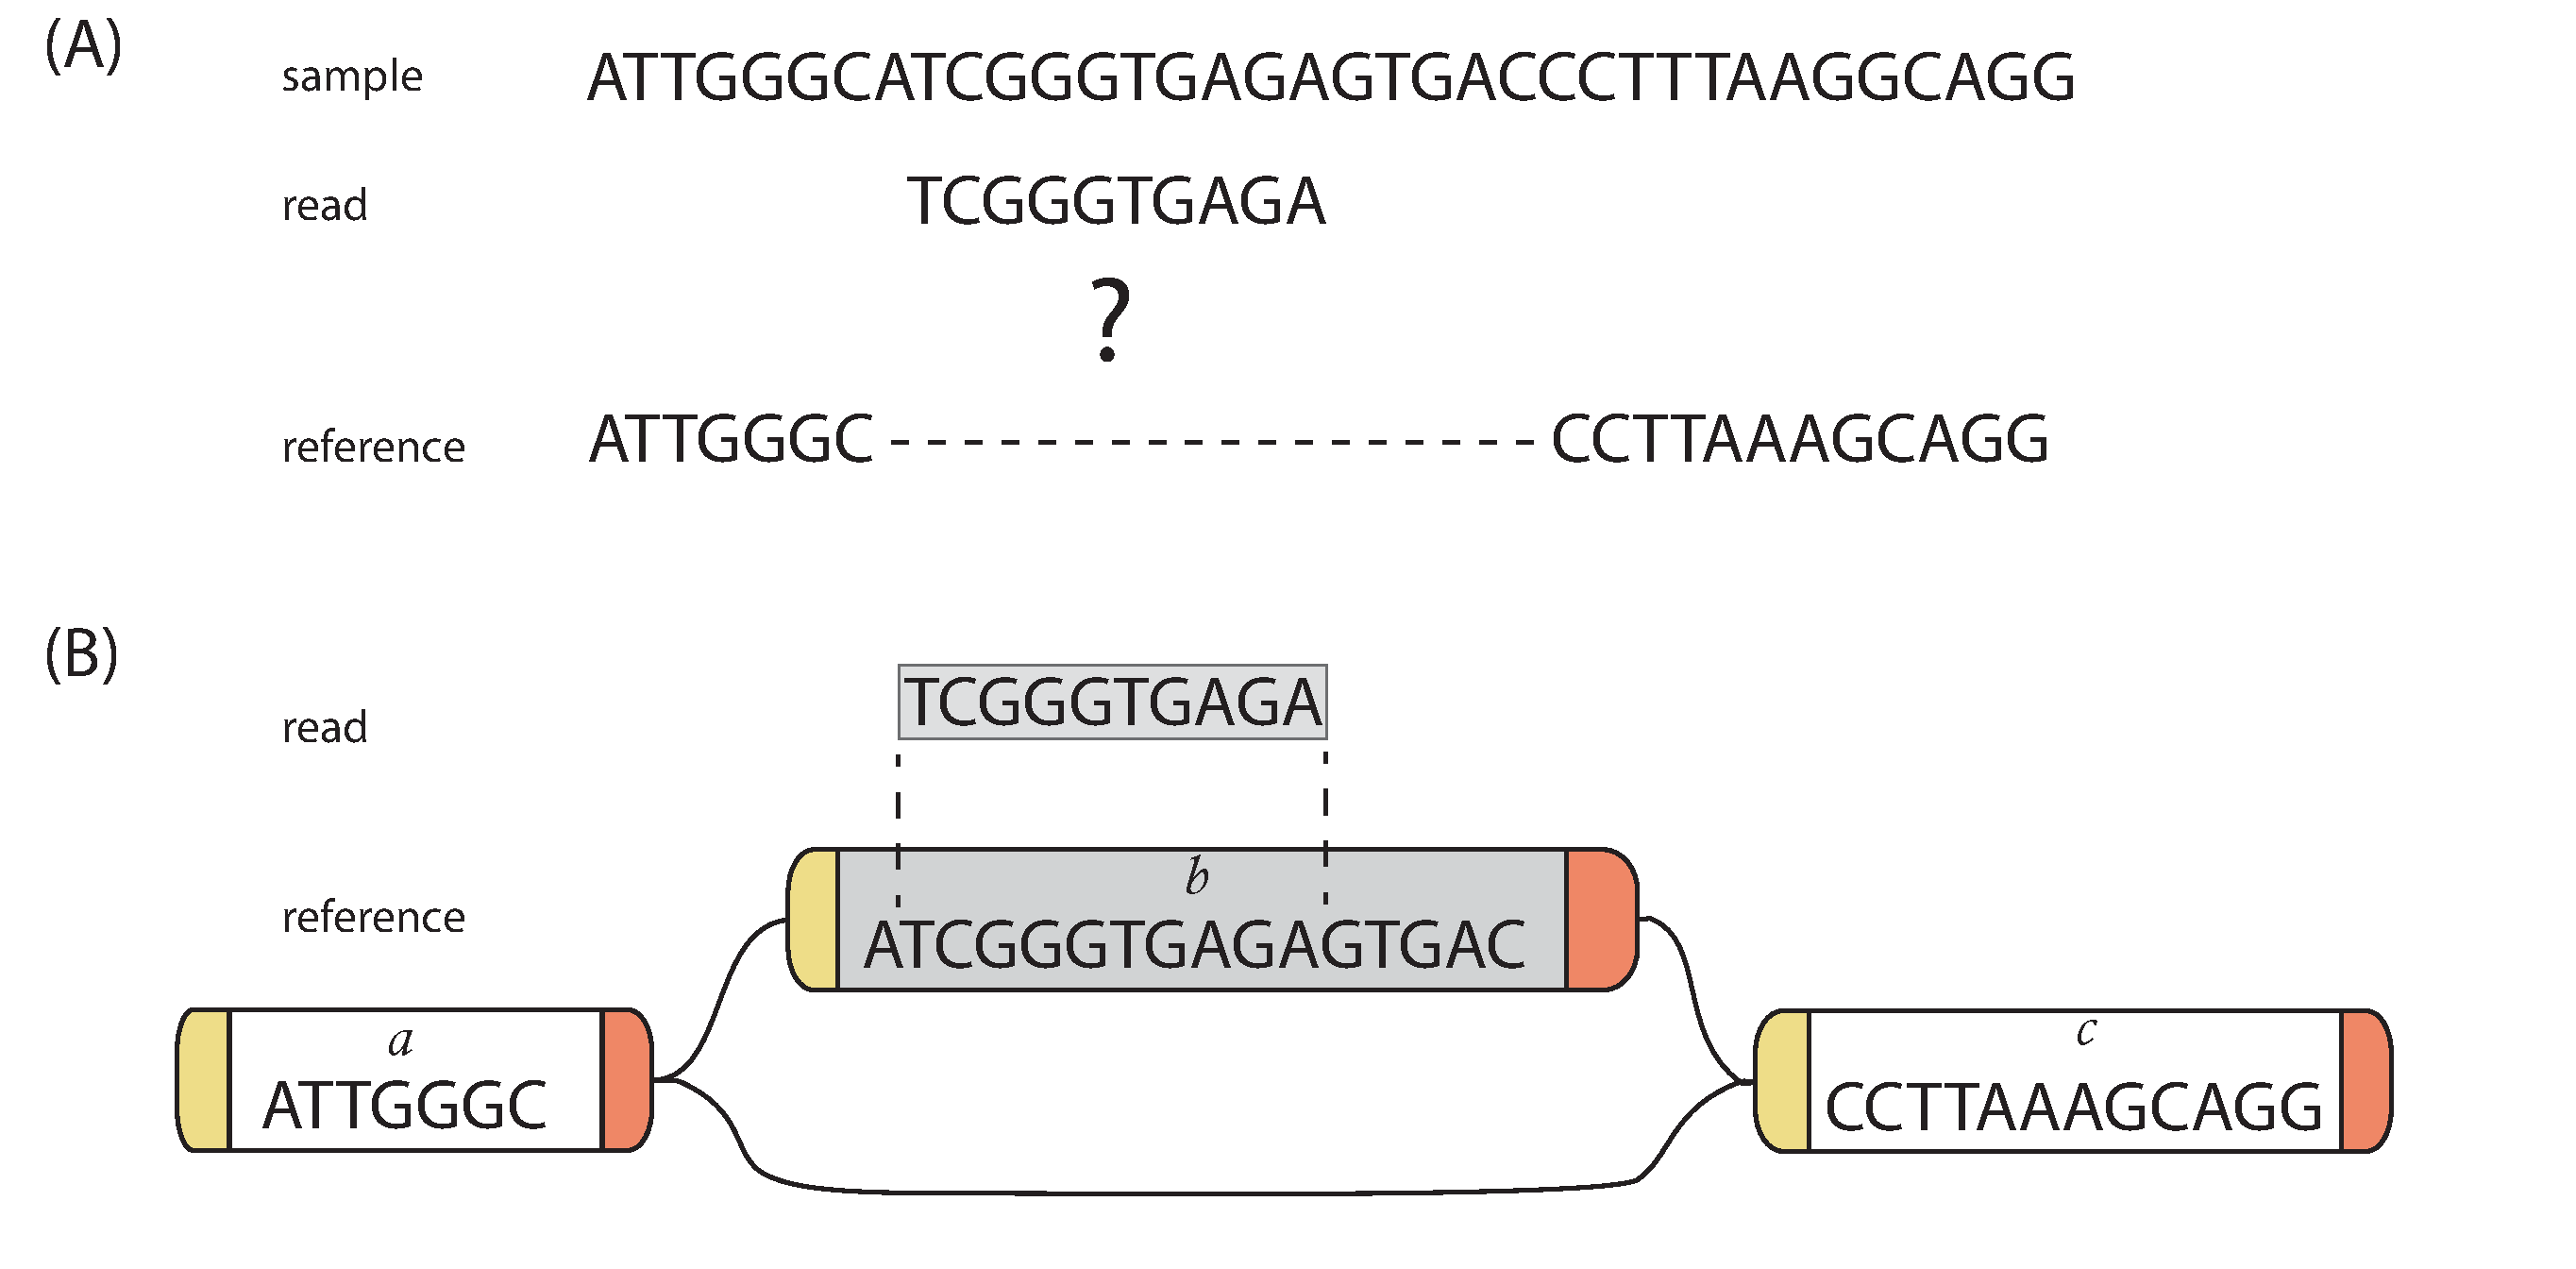
\includegraphics[width=\columnwidth]{mapping_example.pdf}
    \caption[Reference bias in mapping]{\textbf{Reference bias in mapping.} (A) Mapping a read to a linear reference can fail if the sample has a large insertion relative to the reference. (B) Mapping to a pangenome that contains the variant sequence is more likely to succeed.}
    \label{fig:mapping_example}
\end{figure}


This reference bias can be mitigated by using a reference genome containing sequences that more closely resemble the sample of interest.
There have been many proposals for how a reference can accomplish this.
Rather than using a linear reference that is a mosaic of several individuals, such as GRCh38, the reference could be an ancestral genome that contains the most recent common ancestral allele at each locus, or a consensus genome that contains the most common allele at each locus \cite{ballouz_is_2019}.
Another alternative is to use a national or ethnic genome to represent a specific population \cite{ballouz_is_2019,chinese_national_genome_2023,korean_national_genome_2016,vietnamese_national_genome_2015,danish_national_genome_2015,swedish_national_genome_2018,kowal_race_2019}.
But while a population-specific reference may better capture variants that are frequent in that population, the benefit of such a reference will be minimal.
Most human genetic variations occur across populations, rather than being specific to individual populations \cite{nih_understanding_2007}, meaning that even when using a population-specific reference, the majority of the genome will still be subject to the same reference bias as would stem from using any randomly selected reference genome. 
%Furthermore, most human genetic variations are rare so no single reference scaffold will be able to represent all people equally. 

\section{Towards a human reference pangenome}

Pangenomes have previously been proposed to mitigate reference bias \cite{li_building_2010} but until recently, it has not been feasible to create a global human reference pangenome.
The creation of such a resource requires several components: the ability to generate reference-quality genome assemblies and the ability to select genomes to represent the genetic diversity in human population.
Recent advances in genome sequencing technologies, genome assembly algorithms, and a greater understanding of human population genetics have brought this prospect closer to reality.

\subsection{Sequencing technologies}
\label{sec:background:sequencing}

The earliest DNA sequencing techniques, including Sanger sequencing and Maxam-Gilbert sequencing, produced reads on the order of tens of base pairs \cite{sanger_sequencing_1975,sanger_sequencing_1977,maxam_sequencing_1980}.
Sanger sequencing became the basis of the first sequencing machines, which were able to produce reads hundreds of base pairs in length \cite{sequencing_review_2016}.
Sanger sequencing has low throughput but it is highly accurate and it is still used for targeted sequencing of small regions.
These early sequencing technologies are collectively known as "first-generation sequencing".

The next generation of sequencing technologies, known as "next-generation" or "second-generation" sequencing, parallelized the sequencing reactions to greatly increase throughput \cite{sequencing_review_2016}. 
Illumina sequencing has become the dominant next-generation sequencing technology.
Illumina reads have a major advantage of producing paired end reads comprised of two short sequences with a known approximate distance between them.
Modern Illumina sequencing machines can produce millions or even billions of paired end reads with lengths between $100$ and $300$ base pairs in a single run \cite{illumina_sequencing_nodate}.
These reads are generally very accurate with most errors being substitution errors.

Although Illumina has been the most prominent short read sequencing technology \cite{sr_review_2025}, the recent expiration of several of Illumina's patents has led to new emerging technologies.
Element Biosciences' Aviti platform produces reads with a similar lengths and throughput as Illumina reads but with higher accuracy \cite{element_sequencing_2024}. 
Ultima Genomics' UG 100 Platform is a low-cost option for short reads of $~300$ base pairs \cite{ultima_sequencing_2022}. 
Other new technologies include MGI's DNBseq, Pacific Bioscience's Onso, Singular Genomics' G4, and Thermo Fisher Scientific's Ion Torrent \cite{sr_review_2025}.

The term "third-generation sequencing" is generally associated with long read, single molecule sequencing.
Sequencing is performed on individual molecules of DNA, without a separate amplification step \cite{sequencing_review_2016}.
Currently, the two predominant long read sequencing technologies are single-molecule real-time (SMRT) sequencing and nanopore sequencing \cite{lr_review_2023}.
Pacific Biosciences' (PacBio) SMRT sequencing-based High Fidelity (HiFi) reads are between 10 and 25~kbp long with accuracy of up to 99.95\% \cite{pacbio_2019,lr_review_2023}.
Nanopore sequencing machines from Oxford Nanopore Technologies can produce sequencing reads on the order of 10-100~kbp in length, and up to 1~mbp \cite{nanopore_ultralong_2018}, with accuracy of over 99\% \cite{nanopore-fly-accuracy_2024, damaraju_long-read_2024}.

Some sequencing technologies can also capture information from the genome beyond the nucleotide sequence.
Nanopores are capable of detecting DNA base modifications such as methylation \cite{wang_nanopore_2021}. 
Chromosome conformation capture techniques, such as Hi-C, capture the spacial proximity of pieces of DNA \cite{lieberman_hic_2009}. 
Strand-seq is a technique to sequence individual strands of DNA within single cells \cite{sanders_strandseq_2017}.

%Briefly, Sanger sequencing uses fluorescently-labelled nucleotides that stop DNA extension during DNA polymerization, resulting in random-length fragments of DNA that are terminated with a labelled nucleotide. 
%The fragments are then separated by length using gel electrophoresis and the nucleotide at each position is detected from the fluorescent label \cite{sanger_sequencing_1977}. 

%In Illumina sequencing, adapter sequences are ligated on each side of a DNA fragment, which bind to complementary oligonucleotides on a flow cell.
%The fragments are clonally amplified and each copy remains tethered to the flow cell to create clusters of identical fragments, which are then sequenced using a sequencing-by-synthesis technique that adds fluorescently-labelled nucleotides one at a time \cite{shendure_illumina_2008}.
%The DNA fragments are sequenced from both sides, producing paired end reads comprised of two short sequences and an approximate distance between them.

%SMRT sequencing, developed by Pacific Biosciences (PacBio), uses hairpin adapters to circularize a double stranded fragment of DNA, which can be sequenced multiple times in a single pass \cite{pacbio_2019}.

%The other major long read sequencing technology, nanopore sequencing, uses an electric current to drive a DNA molecule through a nanopore embedded in a membrane.
%The current across the membrane changes according to the sequence that is passed through the nanopore, and the change in current can be translated into the DNA sequence using base calling algorithms \cite{wang_nanopore_2021}.



\subsection{Genome assembly}

Advancements in sequencing technologies have driven improvements in the genome assemblies made from them.
Modern long read assembly algorithms are capable of resolving repetitive and complex regions of the genome and can produce higher quality and more contiguous assemblies than short read methods \cite{cheng_hifiasm_2021,rautiainen_verkko_2023,shafin_shasta_2020}.
Haplotype phasing, the problem of distinguishing between the maternal and paternal haplotype, can be done using chromosome conformation capture reads, ultra-long nanopore reads, or sequencing data from the parents \cite{cheng_hifiasm_2021}.
The cost of sequencing and assembling a high-quality phased human genome using these methods was recently estimated to be between ten and fifteen thousand dollars \cite{miga_envisioning_2023}.
\citet{li_assembly_2024} outlines recent advances in the field of genome assembly.

\subsection{Surveys of human genetic variation}

While the Human Genome Project provided a deep understanding of a single human genome, other large-scale projects aimed to provide a broad understanding of the genetic landscape of the human population \cite{international_hapmap_consortium_international_2003,international2005haplotype,1000_genomes_project_consortium_map_2010,1000gp_2015,chaisson_sv_2019}.
These projects have granted us a greater insight into human genetic variation, its role in functional biology, disease, and evolution, as well as its distribution across the globe.
In particular, the International HapMap project \cite{international_hapmap_consortium_international_2003,international2005haplotype} and the later 1000 Genomes Project \cite{1000_genomes_project_consortium_map_2010,1000gp_2015} produced catalogs of variants from thousands of individuals across diverse populations, and have been estimated to have cataloged over $99\%$ of common variants \cite{miga_need_pangenome_2021}.
This greater view of human genetic diversity both highlights the shortcomings of the human reference genome and provides guidance for how to create a reference that better represents all of humanity \cite{ballouz_is_2019,miga_need_pangenome_2021}.

%Projects such as the dbSNP database \cite{sherry_dbsnp_2001}, International HapMap Consortium \cite{international_hapmap_consortium_international_2003,international2005haplotype}, ENCyclopedia of DNA Elements (ENCODE) project \cite{encode_project_consortium_encode_2004}, 1000 Genomes Project \cite{1000_genomes_project_consortium_map_2010,1000gp_2015}, and Human Genome Structural Variation Consortium (HGSVC) \cite{chaisson_sv_2019}

\section{Pangenomes}
\label{sec:background:pangenomes}

A pangenome is an alternative to a standard linear genome.
Pangenomes are collections of genome sequences from a population and the alignments among them.
Because they can represent multiple sequences at each locus, they can better represent variations in a population and have been shown to reduce reference bias relative to using a linear genome \cite{sherman_pan-genomics_2020,noauthor_computational_2016,hprc_pangenome_2023}.
With recent advances in genome sequencing and assembly, coupled with our current understanding of population genetics, it is now feasible to generate reference-quality genome assemblies at the scale and scope necessary for creating a representative human reference pangenome.

The first human reference pangenomes are just beginning to be produced.
The Human Pangenome Reference Consortium (HPRC) has built on the work of the Human Genome Project, the 1000 Genomes Project, and other sequencing projects to begin to establish a global human reference pangenome \cite{hprc_2022}.
The HPRC aims to produce a pangenome comprised of at least 350 individuals' genomes selected to maximally represent the genetic variation present in the human population \cite{hprc_2022}.
The initial draft of the HPRC's human reference pangenome contained the existing GRCh38 and CHM13 reference genomes as well as high-quality (average quality value of 53.57), phased, and annotated genomes of 47 individuals selected from existing 1000 Genomes Project cell lines for their coverage of genetic variants and biogeographic origin \cite{hprc_pangenome_2023}.
The HPRC released three different alignments of these haplotype sequences, constructed using the Minigraph \cite{li_minigraph_2020}, Minigraph-Cactus \cite{minigraph_cactus_2024}, and PanGenome Graph Builder (PGGB) \cite{pggb_2024} pipelines (see Section \ref{sec:graph-construction}). 

In addition to this global pangenome project, there have been several recent efforts to establish ancestry-specific pangenomes for underrepresented populations \cite{pacific_pangenome_2024,chinese_pangenome_2023,arab_pangenome_2024}.
These pangenomes have been curated to represent the genetic diversity of Pacific, Chinese, or Arab populations.
For example, the Chinese pangenome sampled individuals from the 36 of the 55 officially recognized ethnic minority groups and 8 linguistic groups, with the goal of eventually representing all recognized minority groups as well as unrecognized groups \cite{chinese_pangenome_2023}.
These population-specific efforts aim to improve understanding of genetic variants and diseases that are specific to or more frequent in each population.


\subsection{Variation graphs}
\begin{figure}
    \centering
    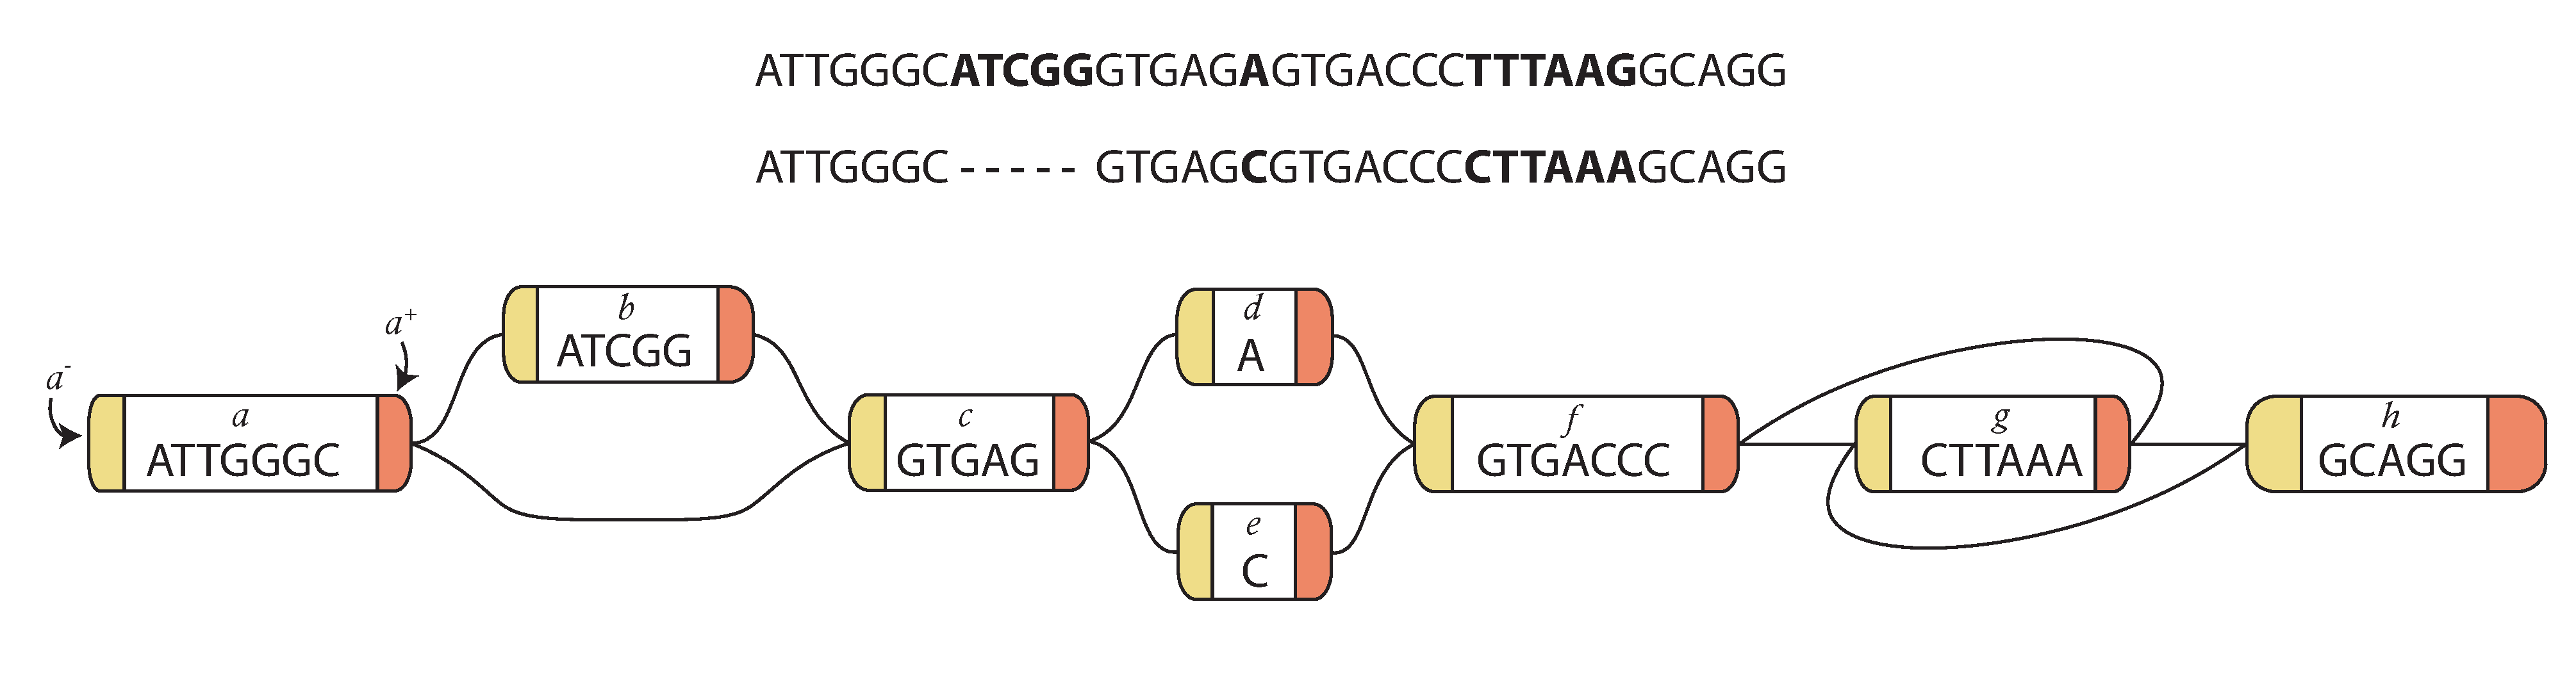
\includegraphics[width=\columnwidth]{example_graph.pdf}
    \caption[Sequence and variation graphs]{\textbf{Sequence and variation graphs}. (A) A sequence graph representing two input sequences. Variations between the two sequences (in bold) are represented as bubbles in the graph. Each node in the sequence graph has a left (-) and right (+) side. Edges connect node sides. (B) The variation graph representation of the input sequences is comprised of the sequence graph and embedded haplotype paths through the graph representing the input sequences.}
    \label{fig:example_graph}
\end{figure}

The sequence content of a human pangenome can easily reach hundreds of billions of base pairs and compact data structures are needed to efficiently represent all of the sequences and the relationships among them. 
\citet{eizenga_pangenome_2020} reviews several methods for representing pangenomes using graph structures.
In this dissertation, I will build upon methods that use sequence graph and variation graph representations of pangenomes \cite{garrison_vg_2018} (Figure \ref{fig:example_graph} A).
Nodes in a sequence graph are labeled with nucleotide sequences and longer sequences can be encoded as paths through the graph.
Divergences in the graph represent variations in the sequences.

Formally, a sequence graph is a bidirected graph $G = (V, E)$ where $V$ is the set of nodes and $E$ is the set of edges.
A node $v$ in a bidirected graph has two node sides, $\{v^{-}, v^{+}\}$, which are arbitrarily designated as ``left'' and ``right'' respectively (Figure \ref{fig:example_graph} A).
Each node $v$ in a sequence graph is labeled with a nucleotide sequence.
Edges in sequence graphs connect node sides; traversals of nodes must enter and exit the node at opposite sides.
A left-to-right traversal of a node is designated as a ``forward'' traversal and the nucleotide sequence is read in the forward direction; a right-to-left traversal is designated as a ``backward'' traversal and the nucleotide sequence is read as its reverse complement.

Variation graphs are sequence graphs that additionally encode a set of reference paths through the graph (Figure \ref{fig:example_graph} B).
These paths provide a stable linear coordinate system and are particularly useful for projecting pangenomic results back to the standard linear reference genome.
They are also useful for restricting walks through the graph to those corresponding to known biological sequences.

\subsection{Variation graph representations}

Standardized representations of sequence graphs are important to allow interchange between tools.
Most pangenome tools support Graphical Fragment Assembly (GFA) format for representing a reference pangenome graph \cite{eizenga_pangenome_2020}. 
A version of the GFA format, the reference GFA (rGFA) format, has been proposed as a stable reference coordinate system that extends that of the linear reference genome \cite{li_minigraph_2020}. 

The variation graph toolkit (\texttt{vg}) is a software suite for working with variation graphs \cite{garrison_vg_2018}.
All of the work presented in this dissertation is implemented as part of the \texttt{vg} toolkit.
\texttt{vg} originally supported two formats for representing variation graphs: the original VG format and XG format \cite{garrison_vg_2018}.
Although the XG format is more memory-efficient than VG, it is a static format that does not allow for modifications.
Three other memory-efficient, dynamic formats were later introduced: ODGI \cite{guarracino_odgi_2022}, HashGraph, and PackedGraph \cite{eizenga2020efficient}.
VG, XG, HashGraph, and PackedGraph formats efficiently represent the sequence graph component of a variation graph but are less efficient for storing paths, and generally only a small number of reference haplotypes are included.
The vg toolkit uses the Graph Burrows Wheeler Transform (GBWT) format for storing the full set of reference haplotypes for a variation graph \cite{siren_indexes_2020}.
A GBZ represents a GBWT and the node sequences of the graph to represent the subgraph of the variation graph whose edges are supported by haplotype sequences \cite{siren_gbz_2022}.

Graph indexes are discussed in Section \ref{sec:graph-mappers}.

\subsection{Graph construction methods}
\label{sec:graph-construction}

A variation graph can be constructed using a variety of different methods, each of which produces graphs with distinct characteristics.
One option for constructing a graph is to start with a set of variants, typically represented in a variant calling format (VCF) file.
The \texttt{vg} toolkit's \texttt{vg construct} tool takes a reference and a set of variants called against that reference as input and produces a variation graph.
Variation graphs constructed with this method are generally topologically simple. 

Graphs can also be constructed from phased genome assemblies.
There are currently three methods for constructing pangenome graphs from assemblies.
The Minigraph algorithm starts from a single reference genome and progressively aligns and incorporates each additional genome into the graph \cite{li_minigraph_2020}.
As this algorithm is not designed to find small variants, graphs constructed with Minigraph represent only larger structural variants and are generally simple and acyclic \cite{li_minigraph_2020}.
The Minigraph-Cactus pipeline builds on graphs constructed with the Minigraph algorithm and adds smaller variants using the Cactus algorithm \cite{minigraph_cactus_2024}. 
This introduces smaller variants, nested variants, and can create cycles in the graph.
The PanGenome Graph Builder (PGGB) algorithm constructs a graph using a reference-free all-to-all comparison of genomes \cite{pggb_2024}.
The PGGB pipeline tends to add more alignments between homologous sequences, particularly copy number variants, resulting in collapsing of repetitive sequences into a single copy \cite{hprc_pangenome_2023}.
This creates large cycles and complicated nested structures.

The choice of graph construction method is a trade off between the complexity of the graph and the homology that they represent.
PGGB graphs are the most topologically complicated, but the construction method is unbiased by the choice of reference and the collapsing of variants better represents the relationship between paralogous sequences within a genome.
In contrast, less collapsed graphs built with Minigraph are simpler and can more clearly define the orthology among genomes, as the individual repeat copies are separately expressed and aligned \cite{li_minigraph_2020}. 


\subsection{Snarl decomposition}

To help find organization in a sequence graph, it is often useful to describe common topological motifs.
A simple variation such as a single nucleotide polymorphism (SNP) or and insertion or deletion (indel) will be represented by one or two nodes representing the variant sequences, flanked by two nodes representing conserved sequences.
In Figure \ref{fig:snarl_tree} A, node $l$ represents an insertion that may be skipped by taking the edge between nodes $k$ and $m$.
Nodes $k$ and $m$ represent conserved sequences that flank the indel.
The subgraph between node sides $k^+$ and $m^-$ is called a snarl.
A snarl is defined by a pair of node sides, $\{x^{-/+}, y^{-/+}\}$, that delimit a subgraph between them.
The nodes $x$ and $y$ are referred to as the boundary nodes of the snarl.
Two node sides define a snarl if they are (i) separable: splitting the boundary nodes into their two node sides disconnects the snarl from the rest of the graph, and (ii) minimal: there is no node $z$ within the snarl that is separable with the boundary nodes.
%I will use the term ``snarl'' to refer to the two boundary nodes and the subgraph between them.

Snarls frequently occur successively with a shared boundary node between them.
A sequence of consecutive nodes and snarls is called a ``chain''.
In Figure \ref{fig:snarl_tree} A, node $e$, snarl $\{e^+$, $g^-$\}, node $g$, snarl $\{g^+$, $j^-\}$, and node $j$ form in a chain $\{e$, $j\}$.
Because chains contain entire nodes, I define them here by a pair of nodes rather than by a pair of node sides as for snarls.
%Actually the definition should probably involve directionality or something to cover looping chains but I think that would be unnecessarily complicated

Snarls and chains may be nested within each other.
Conceptually, this can occur when multiple variants affect the same locus, such as an insertion that contains a SNP.
In a graph, a snarl contains another snarl if all of the nodes in the latter snarl are contained in the subgraph of the former.
A snarl contains a chain if it contains all of the chain's component snarls.
In Figure \ref{fig:snarl_tree} A, the chain $\{e$, $j\}$ is contained in the snarl $\{a^+$, $k^-\}$.

%A sequence graph can be entirely decomposed into nested snarls and chains.
The nesting relationship of snarls and chains of a graph is described by its ``snarl tree'' (Figure \ref{fig:snarl_tree} A).
Each node, snarl, and chain in the graph is represented as a node in the snarl tree.
A chain is a child of a snarl if it is contained in the snarl and no other descendant of the snarl.
A node or snarl is a child of a chain if it is a component of the chain.
Every node and snarl is a child of a chain; a chain containing just one node is called a ``trivial chain''.
Because of this, the snarl tree is composed of alternating layers of snarls and chains, usually starting with a top-level chain as the root.

Nodes, snarls, and chains all have the property that they are connected to the rest of the graph by two node sides.
Based on this property, snarls and chains can be treated as nodes within their parents, obscuring the presence of a subgraph between the boundaries of the child.
A ``netgraph'' is a view of a snarl where its child chains are replaced by nodes.
In Figure \ref{fig:snarl_tree} C, the snarl $\{a^+$, $k^-\}$ has been replaced with its netgraph.

\begin{figure}[htp]
    \centering
    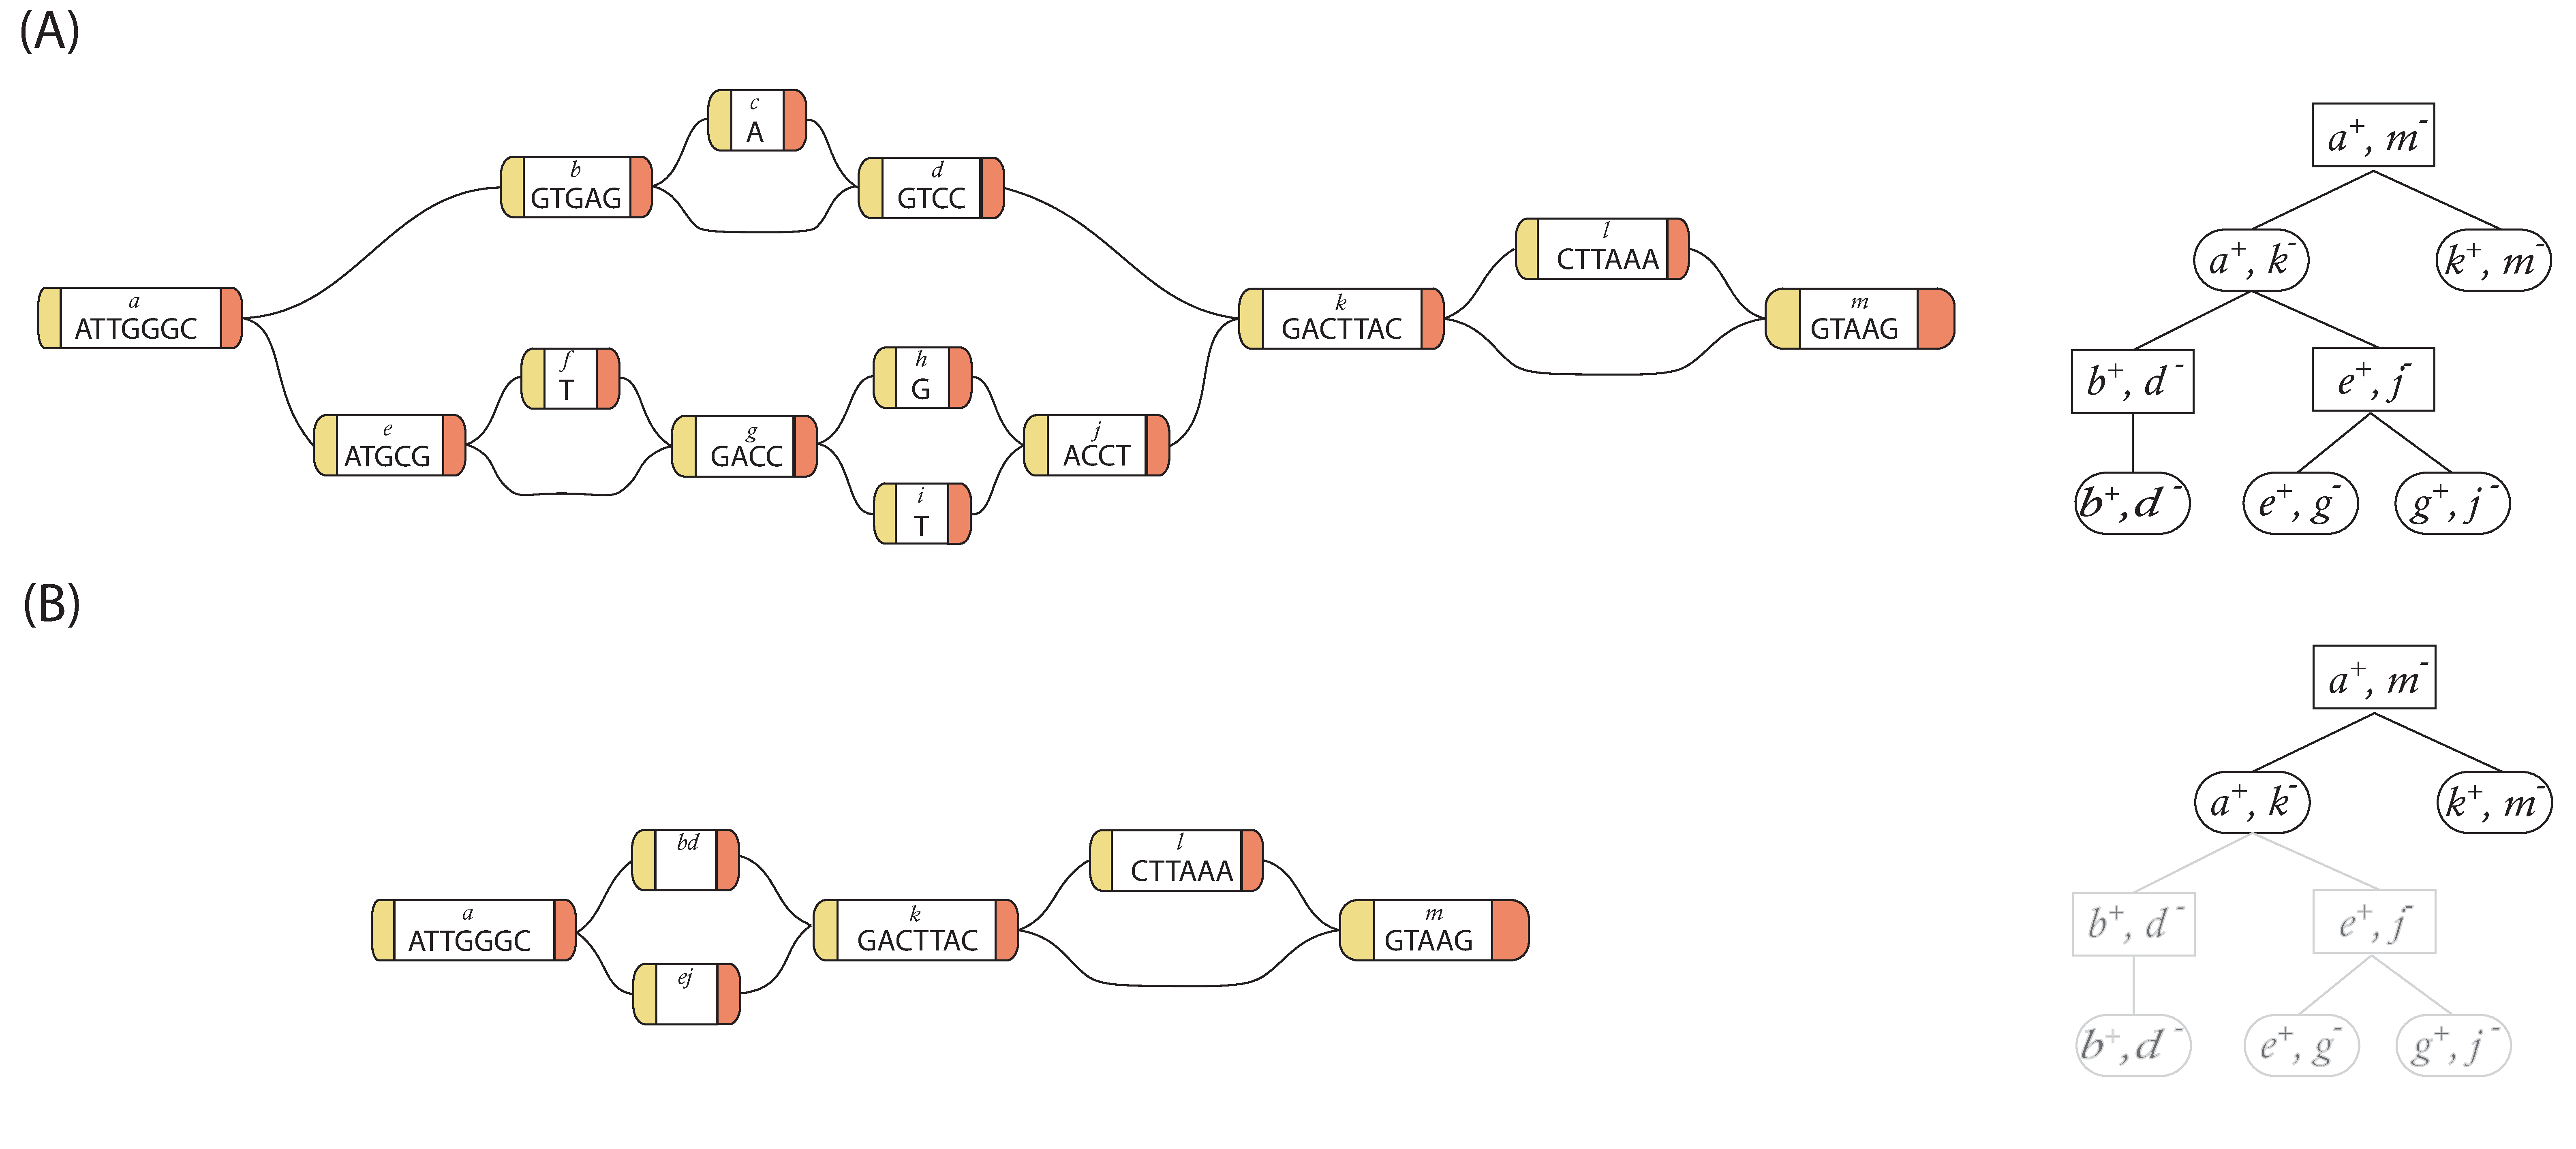
\includegraphics[width=0.8\columnwidth]{snarl_tree.pdf}
    \caption[The snarl decomposition]{\textbf{The snarl decomposition} (A) A sequence graph (left) and its corresponding snarl tree (right). Chains are represented by rectangular nodes in the snarl tree; snarls are represented by elliptical nodes. For simplicity, nodes are not shown on the snarl tree.
    (B) Snarls $\{a^+$,$k^-\}$ and $\{k^+$,$m^-\}$ highlighted in the graph and snarl tree. (C) Chains $\{b$, $d\}$ and $\{e$, $j\}$ are highlighted in the variation graph and snarl tree. Below, a view of the graph with snarl $\{a^+$,$k^-\}$ replaced by its netgraph. In this view, the snarl's child chains $\{b$, $d\}$ and $\{e$, $j\}$ are represented by nodes.}
    \label{fig:snarl_tree}
\end{figure}

\section{Read mapping}
\label{sec:background:mapping}

Read mapping is often the first step of a genomic pipeline.
The problem of read mapping is to take sequencing reads from a sample and find a placement of the reads in a reference, usually as a base-level alignment to the reference.
The terms ``mapping'' and ``alignment'' are often used interchangeably.
For the sake of clarity, I will use ``mapping'' to refer to the problem of finding the location of a read in a reference, and ``alignment'' to refer to the problem of finding the optimal base-level alignment.
Alignment is typically a component of a mapping algorithm, used to find the optimal alignment to a smaller region of the reference.

Most mapping algorithms follow a common seed-and-extend framework comprised of three main steps.
In the first step, seeding, short ``seed'' alignments are found between the read and reference (Figure~\ref{fig:mapping_overview} A).
Next, the seeds may be grouped together based on their locations in the reference to identify regions of the genome that are likely targets of mapping.
This step is either done by clustering  (Figure~\ref{fig:mapping_overview} B ) or chaining  (Figure~\ref{fig:mapping_overview} C), and is omitted entirely by some mappers.
In clustering, partitions of seeds are found such that seeds that may originate from the same mapping are placed in the same partition.
Chaining algorithms find ordered sets of co-linear seeds that occur in the same order in the read and reference. 
Once a likely location is found on the reference, the final alignment step is done (Figure~\ref{fig:mapping_overview} D, E).
In this step, the seed alignment is extended using a dynamic programming algorithm to find the final base-level alignment.

Read mapping algorithms differ depending on the type of input reads and whether the target reference is a linear genome or a graph.
Earlier algorithms were designed to align shorter reads to linear genomes.
These algorithms were later adapted to align longer reads and to align to graph references.

\begin{figure}
\centering
\includegraphics[width=0.8\columnwidth]{mapping_algorithm_overview.pdf}
\caption[Seed-and-extend mapping algorithm overview]{\textbf{Seed-and-extend mapping algorithm overview} (A) Short seed alignments between the read and reference are found using a text index or $k$-mer index. Seeds are grouped together into unordered clusters (B) or ordered chains (C). Alignment is done from individual seeds (D) or between seeds in a chain (E).}
\label{fig:mapping_overview}
\end{figure}


\subsection{Seeding}

Existing liner mappers generally use either $k$-mer indexes or suffix tree-based text indexes for seeding \cite{li_survey_2010,sahlin_survey_2023}.

%also Slider, which uses merge sorting

\subsubsection{$k$-mer indexes}

$k$-mer based algorithms use an index that stores the locations of $k$-mers (subsequences of length $k$) in the reference, then look up $k$-mers from the read to find matches in the reference.
$k$-mer indexes are often stored in a hash table, and these indexes are sometimes referred to as hash-based indexes.
Rather than storing the locations of every $k$-mer in the reference, many algorithms use different schemes for selecting a subset of $k$-mers to be stored in the index \cite{li_minimap2_2018,lee_mosaik_2014,jain_mashmap_2018, edgar_urmap_2020,edgar_syncmers_2021}.
For a scheme to be effective for seeding alignments, it must sparsely sample the reference to reduce the size of the index, evenly sample sequences so that the gap between two consecutive seeds is small, and consistently sample sequences so that if two sequences are similar, then the $k$-mers selected will be the same \cite{marcais_improving_2017}.

Minimizers are used by several mappers as a method for selecting $k$-mers.
A minimizer scheme is defined by two parameters, $k$ and $w$, and a function $f$ that determines an ordering of the $k$-mers.
Within a window of $w$ consecutive $k$-mers, the minimizer is the $k$-mer with the lowest value according to $f$.
Commonly used ordering functions include lexicographic order, random hash functions, and other functions optimized to improve the density of minimizers in the reference \cite{zheng_minimizers_2020,marcais_minimizers_2018}.
A minimizer index stores the locations of minimizers from all windows in a sequence.
If two sequences share a subsequence of length at least $w+k-1$, then they are guaranteed to share a minimizer.

Minimizers can be further prioritized based on their frequency in the reference, improving the number of false-positive matches \cite{jain_winnowmap_2020}.
Prioritizing low frequency or high confidence seeds can also help prioritize reference alleles to map a read to the correct repeat copy. 
This can be an advantage when the mapper would otherwise have mapped to a repeat with a better alignment to the read, but with fewer unique matches with the reference \cite{winnowmap2_2022}.
%Winnowmap also tries to pick the same minimizer in a run of the same minimizer
%Winnowmap2 does a first extension step to get minimal confidently alignable substrings (MCASs), which help it prioritize reference alleles, which are assumed to flank variants in the read in repeat units

Some $k$-mer methods allow inexact matches, also known as fuzzy seeds.
Spaced $k$-mers allow substitutions in $k$-mers by allowing certain positions in the $k$-mer to be mismatches \cite{ma_patternhunter_2002}.
Similarly, strobemers are used to find seeds across indels by linking multiple $k$-mers within a window together \cite{sahlin_strobemers_2021}.

%Syncmers are another alternative to minimizers that selects $k$-mers based on the properties of the $s$-mers within a $k$-mer \cite{edgar_syncmers_2021}.
%Unlike minimizers, syncmers are selected solely based on the $k$-mers and do not depend on their context.
%A universal hitting set (UHS) is an set of $k$-mers that is guaranteed to have a $k$-mer for any sequence of length $L$ \cite{ekim_randomized_2020,orenstein_compact_2016}.
%Although UHSs are theoretically useful, computing them is a difficult problem.


\subsubsection{Text indexes}

Text indexes provide two basic operations: counting occurrences of a substring within a template string and locating their positions.
Suffix tries, suffix trees, and suffix arrays are data structures that index all suffixes of a template string \cite{li_survey_2010}.
Because any substring of a template string must be a prefix of one of its suffixes, these suffix indexes can be used to find exact matches in a simple linear search.
Suffix trees and suffix arrays have memory costs linear in the size of the template and support locate queries in time linear in the length of the query.
The FM-index uses a Burrows Wheeler Transform (BWT) to improve upon the memory cost while maintaining the fast substring queries.
The Burrows-Wheeler Transform (BWT) is found by sorting all rotations (a transformation of a string taking a prefix and moving it to the end of the string) of the template string, then taking the last character from each rotation \cite{burrows_wheeler_1994}.
Because characters in the BWT are grouped according to their context, there tend to be long runs of the same character originating from repetitive regions, making the BWT highly compressible and especially useful for indexing a reference genome.


%This should maybe go in the graph section but it's easier to read here
While the BWT is common for indexing a single genome, the memory cost is still too high to be practical for indexing multiple reference genomes.
The Run-Length FM-Index (RLFM-index) can index multiple genomes, represented as a single concatenated sequence, with a memory requirement linear in the number of runs in the BWT \cite{makinen_succinct_2005,makinen_storage_2010}.
Because genome sequences are highly similar and repetitive, the RLFM-index can store many genomes with low memory, but using this index to locate substrings requires an additional data structure that increases memory requirement.
This problem remained unsolved until the $r$-index was developed a decade later.
The $r$-index can find exact matches in time linear in the length of the query plus the number of occurrences, using an index whose size is linear in the number of runs in the BWT \cite{gagie_rindex_2020}.
The $r$-index makes it feasible to index and search databases of whole genomes \cite{rossi_moni_2022}.

Many existing mappers use suffix trees \cite{kurtz_versatile_2004}, suffix arrays \cite{abouelhoda_replacing_2004,hoffmann_fast_2009}, or FM indexes \cite{langmead_bowtie2_2012,li_bwa_mem_2013,li_soap2_2009,li_bwa_2009,langmead_bowtie_2009} to find exact matches as seeds.
Unlike $k$-mer based methods, text indexes can produce variable-length seeds.
These are often maximal exact matches (MEMs), which are exact matches that cannot be extended further on either side without a mismatch.

%MEMs, MUMs, SMEMs, etc


%A simple example of a text index is a suffix trie, which stores all suffixes of a template string in a tree structure where edges are labeled with characters such that each suffix is represented in a path from the root of the tree down to a leaf \cite{li_survey_2010}.
%Because any substring of the template string must be a prefix of one of its suffixes, exact substring queries can be done in a walk down from the root of the suffix trie in time linear to the length of the query string.
%Suffix trees represent the same information as suffix tries with reduced memory by compressing non-branching paths and replacing the characters with offsets in the original template string. 
%A suffix array further reduces the memory use by representing a vector of integers to implicitly represent the tree structure.
%A suffix array represents the sort order of all suffixes of a template string.
%Using a suffix array, substring query can be done in a binary search in $O(Q + logT)$ time, where $Q$ is the length of the query and $T$ is the length of the template \cite{suffix_array_1993}. 
%The Burrows-Wheeler Transform (BWT) is found by sorting all rotations (a transformation of a string taking a prefix and moving it to the end of the string) of the template string, then taking the last character from each rotation \cite{burrows_wheeler_1994}.
%The BWT is reversible, highly compressible, and, using an additional data structure called the FM-index, can perform exact match queries in time linear in the length of the query \cite{fm_index_2000}.
%The FM-index's memory requirement scales with the size of the template sequence, and while it has been instrumental in indexing the single human reference genome, it doesn't scale to collections of genomes.

\subsection{Clustering and chaining}

After extracting short seed alignments between the read and reference, the seeds are prioritized to avoid performing an expensive dynamic programming step on unlikely seeds.
Some algorithms prioritize individual seeds based on properties of the seed, such as the number of occurrences in the reference  \cite{langmead_bowtie2_2012}, and evaluate them in order of priority.
Others groups seeds by chaining or clustering and evaluate groups of seeds together \cite{li_bwa_mem_2013,li_minimap2_2018,lee_mosaik_2014,jain_mashmap_2018}.
Clustering techniques partition seeds into groups that are near each other on the reference or that are on the same diagonal line in the alignment matrix between the read and reference, in order to identify groups of seeds arising from the same alignment to the reference.

Some mappers, particularly long read mappers, use a chaining step in addition to or instead of clustering \cite{sahlin_survey_2023}.
The goal of chaining is to produce optimal sets of co-linear seeds, meaning that the seeds occur in the same order in the read and the reference.
Chains provide more information than clusters and they are particularly useful for long reads because alignment can be done between consecutive seeds in the chain, instead of out from individual seeds.
Chaining can be solved using a dynamic programming approach to optimize a chain scoring function.
As a representative example used by many mappers, Minimap2 defines the score for a chain ending at the $i^{th}$ seed as follows \cite{minimap2_2021}:
\begin{equation}
    f(i) = \max\begin{cases}
                \max_{i>j\geq 1} \{f(j) + \alpha(j,i) - \beta(j,i)\}\\
                w_i
                \end{cases}
\end{equation}
where $f(j)$ is the best score of a chain ending at the $j^{th}$ seed, $\alpha(j,i)$ is the number of bases that match between seeds $i$ and $j$, $\beta(j,i)$ is the gap cost, and $w_i$ is the score of taking just seed $i$ (the number of bases in the seed) \cite{minimap2_2021}.
Minimap2's scoring function allows overlaps between consecutive seeds but penalizes them. 
The gap cost is based on the difference in distance between the seeds in the read and the distance between them in the reference, as a way of estimating the indels that would be taken in an alignment between the seeds.
Minimap2 uses a concave gap cost, where the additional cost of taking a longer gap decreases as the length of the gap increases \cite{sahlin_survey_2023}.
Concave gap costs favor taking fewer, longer gaps over additional, small gaps, making them more biologically representative than linear gap costs, which increase linearly as the length of the gap increases \cite{sahlin_survey_2023}, but there are optimizations to improve the time complexity of chaining with linear gap cost that can't be used with concave gap costs \cite{abouelhoda_linear_chaining_2005}.


%This recursion can be made more efficient using an auxiliary data structure for finding the best score within a range of previous seeds and a gap cost that can be efficiently computed without considering the sequence content of the read and reference \cite{myers_chaining_1995}.

\subsection{Alignment}

The final base-level alignment is typically found using dynamic programming, either by extending seed alignments or by aligning the entire read to a region of the reference that is found by clustering.
Most standard dynamic programming algorithms are based on the Smith-Waterman-Gotoh algorithm for local alignment \cite{smith_waterman_1981,gotoh_1982} or Needleman-Wunch algorithm for global alignment \cite{needleman_wunsch_1970}.
These algorithms use a rectangular dynamic programming matrix of the score of aligning each base between the query and reference sequences.
The cost of skipping bases in either sequence is defined by the gap cost; most modern algorithms use an affine gap penalty with a relatively high gap open penalty taken for opening any gap, and relatively low a gap extension penalty that is linear in the length of the gap.

Standard dynamic programming algorithms have prohibitive runtimes so many mappers use different optimizations to speed up alignment and to reduce the search space of the dynamic programming matrix.
Some mappers use Single-Instruction Multiple-Data (SIMD) microprocessors to accelerate dynamic programming by parallelizing computation of independent cells in the dynamic programming matrix \cite{farrar_striped_2007,rognes_six-fold_2000}.
Banded alignment algorithms restrict the dynamic programming matrix to a diagonal ``band'' of a specified width, preventing large insertions or deletions that would exceed the width \cite{chao_aligning_1992}.
BLAST's X-drop algorithm fills in the matrix row by row, and stops extending each row when the best possible score is a given value X less than the best score seen in the previous row \cite{altschul_blast_1990}.
This has a similar effect to banded alignment in that it forces the alignment to remain close to the diagonal, preventing large insertions or deletions that could align the start of one sequence to the end of another.

The Wave Front Algorithm (WFA) is a newer alignment algorithm that runs in time parametrized by the similarity between the two sequences \cite{marco-sola_fast_wfa_2021}.
Instead of performing dynamic programming over the length of the sequence, the WFA algorithm runs through the diagonal of the dynamic programming matrix, making it faster for sequences that are similar and whose alignment would be found close to the diagonal \cite{marco-sola_fast_wfa_2021}.
Later advancements to the algorithm reduces the space requirement to be linear in the alignment score \cite{eizenga_wfa_2022}.

%Some mappers don't use dynamic programming, but use a text index allowing inexact matching \cite{langmead_bowtie_2009,li_bwa_2009},

\subsection{Graph mappers}
\label{sec:graph-mappers}

Mapping reads to pangenome graph references is a much newer and far less well studied problem than mapping to linear references.
In general, mapping to graph references is more accurate, but also requires more computational resources, and improving read-to-graph mapping is still an open area of research.
Existing graph mappers generally follow the same seed-and-extend structure as linear mappers, but use graph-specific adaptations for each step \cite{eizenga_pangenome_2020, baaijens_computational_2022}.

Many graph mappers use a $k$-mer index for seeding \cite{rautiainen_graphaligner_2020,rakocevic_fast_2019,vaddadi_vmap_2019,schneeberger_simultaneous_2009}.
$k$-mers can be found within the sequences of nodes, from walks in the graph, or from the reference haplotype sequences. 
Chapter \ref{chapter:sr-giraffe} describes the minimizers of haplotypes used in the mapping tools I helped develop.
Others mappers use generalizations of the BWT for indexing graphs \cite{garrison_vg_2018,kim_hisat2_2019,siren_indexing_2014,siren_indexes_2020} or collections of genomes \cite{rossi_moni_2022}.
%The Generalized Compressed Suffix Array (GCSA) is a BWT-based text index for graphs used by VG MAP to find seeds \cite{siren_indexing_2014,siren_indexes_2020}.

Clustering or chaining seeds in a graph is more difficult than in a linear genome due to the added ambiguity of calculating distance in a graph.
Different tools use a variety of estimations of distance based on embedded linear paths \cite{garrison_vg_2018}, linear coordinates based on the snarl decomposition \cite{rautiainen_graphaligner_2020}, an embedded representation of the graph \cite{vaddadi_vmap_2019}, or by enumerating linear paths through the graph \cite{li_minigraph_2020}.
In Chapter \ref{chapter:distance}, I discuss my work on a snarl-based minimum distance calculation and its use in clustering. 

Many existing graph chaining algorithms are based on an algorithm from M{\"a}kinen et al. that uses a minimum path cover of the graph to determine reachability and distance in directed acyclic graphs (DAGs) \cite{makinen_dag_chaining_2019}.
The cost of this algorithm is parameterized by the width of the graph, making it efficient for most current human pangenome graphs for which a minimum path cover can be achieved with a small number of paths \cite{makinen_dag_chaining_2019}.
Further advancements to this algorithm have extended it to use different gap costs \cite{chandra_gap-sensitive_chaining_2023}, to be recombination-aware by penalizing haplotype switches \cite{chandra_haplotype-aware_2024}, to allow overlaps of one node between seeds \cite{ma_graphchainer_2023}, and to chain through cyclic graphs \cite{panaligner_2024}.

%Minigraph uses a chaining algorithm based on that of Minimap2.
%Minigraph uses two rounds of chaining: it first produces linear chains within individual nodes in the graph, then makes chains of the linear chains taking into account the topology of the graph.
%The second round of chaining finds graph distances by enumerating up to 16 shortest-path walks between between pairs of linear chains.
%Of those paths, it chooses the path with length closest to the gap in the read for computing the gap cost \cite{minigraph_2020}.



Alignment is also more challenging in a graph context, particularly for cyclic graphs.
Many mappers use linear dynamic programming algorithms that have been extended to a graph context.
One such example is partial order alignment (POA), an algorithm for constructing and aligning to multiple sequence alignments \cite{lee_poa_2002}.
Later algorithms have accelerated alignment with POA using SIMD and other optimizations \cite{jain_accelerating_2019,gao_abpoa_2021,darby_vargas_2020}
However, this algorithm and most mappers based on it are limited to aligning to DAGs \cite{kim_hisat2_2019,rakocevic_fast_2019,li_minigraph_2020,ma_graphchainer_2023}.
Other mappers align to cyclic graphs by converting them to DAGs before using an acyclic aligner \cite{garrison_vg_2018} or use graph extensions of linear alignment algorithms \cite{rautiainen_bit-parallel_2019,zhang_fast_2022}. 
%A graph extension of the WFA has been proposed to align similar sequences to sequence graphs more quickly than traditional methods \cite{zhang_fast_2022}.
%VG-MAP can align to graphs of arbitrary topology by ``unrolling'' a graph to convert it to a DAG then using POA \cite{garrison_vg_2018}.
%GraphAligner maps to cyclic graphs using graphs extension of Myers' bit parallel alignment algorithm and the \textit{Shift-And} algorithm for exact string matching \cite{rautiainen_bit-parallel_2019}

Another class of sequence-to-graph aligners use shortest-distance queries to support alignment.
In this paradigm, the problem of minimizing edit distance is viewed as finding the shortest path in an alignment graph that represents edits in an alignment between the query sequence and reference graph.
The shortest path problem can then be solved using the A* algorithm to find the optimal alignment \cite{ivanov_astarix_2020,bonizzoni_recalign_2025}.
This strategy has been extended to allow recombination-aware alignment \cite{bonizzoni_recalign_2025}.


\subsection{Downstream applications of read mapping}

Read mapping is the first step for many genomic analyses including variant calling, genotyping, and transcriptomic analysis. 
Although these methods are not a focus of this thesis, I will briefly summarize some of the tools used in the results that I present.

Small variant calling is typically done by mapping reads then using statistical models to distinguish between sequencing errors and real variants in the sample \cite{bonfiglio_calling_2024}.
DeepVariant is convolutional neural network-based variant caller for calling small variants \cite{deep_variant_2018}. 
In Chapters \ref{chapter:sr-giraffe} and \ref{chapter:lr-giraffe}, I present variant calling results using models of DeepVariant trained on reads mapped to a pangenome graph.

Calling structural variants is a more challenging problem than calling small variants, particularly around highly repetitive regions.
Long reads are capable of spanning breakpoints and repeats and as a result have greatly improved SV calling methods.
Sniffles is a commonly used structural variant caller that uses long reads alignments \cite{smolka_sniffles2_2024}.
While variant calling methods identify new variants, genotyping methods determine the presence of known variants in a sample.
\texttt{vg call} is a graph-based genotyper primarily used for genotyping structural variants \cite{hickey_vgsv_2020}.
It uses read coverage of traversals in the pangenome graph to genotype the variants present in the graph.


\chapter{Distance Indexing}
\label{chapter:distance}

\section{Preface}
This chapter is the full text of my paper "Distance Indexing and Seed Clustering in Sequence Graphs" \cite{chang_distance_2020}, which I presented and ISMB in 2020 and which was published in Bioinformatics.
I am the sole first author of this paper. 
Benedict Paten and David Haussler originally conceptualized the idea of a snarl decomposition-based distance index.
Jordan M. Eizenga contributed to the design of the distance index and provided guidance and support throughout the process of software development and writing.
Jordan M. Eizenga, Adam M. Novak, and Jouni Sirén provided minor contributions to the software development and conceptualization. 

While the majority of my work is done for variation graphs, the distance index is generalizable to sequence graphs as well.
Some notation in this chapter may differ from the rest of the thesis but the underlying structures they describe are the same.
The text contains minor edits to conform with the formatting of this thesis.

\newpage

\section{Introduction}
Conventional reference genomes represent genomes as a string or collection of strings.
Accordingly, these so-called ‘linear reference genomes’ can only store one allele at each locus.
The resulting lack of diversity introduces a systematic bias that makes samples look more like the reference genome \cite{zook_integrating_2014}.
This reference bias can be reduced by using pangenomic models, which incorporate the genomic content of populations of individuals \cite{noauthor_computational_2016}.
Sequence graphs are a popular representation of pangenomes that can express all of the variation in a pangenome \cite{paten_genome_2017}. 
Sequence graphs have a more complex structure and the potential to contain more data than linear genomes.
This tends to make functions on a sequence graph more computationally challenging than analogous functions on linear genomes.

One such function is computing distance.
In a linear genome, the exact distance between two loci can be found by simply subtracting the offset of one locus from the offset of the other.
In a graph, calculating distance is much more complicated; there may be multiple paths that connect the two positions and different paths may be relevant for different problems.

Distance is a basic function that is necessary for many functions on genome graphs; in particular, calculating distance is essential for efficient mapping algorithms.
In a seed-and-extend paradigm, short seed matches between the query sequence and reference are used to identify small regions for expensive alignment algorithms to align to \cite{schneeberger_simultaneous_2009,li_minimap_2016,rakocevic_fast_2019,garrison_vg_2018,vaddadi_read_2019,rautiainen_bit-parallel_2019}. 
Often these regions are identified by clusters of matches. 
Clustering requires repeated distance calculations between seeds and can be very slow in graphs as large as whole genome graphs. 
The prohibitive run time of clustering algorithms can make them impractical for mapping and some mapping algorithms omit this step entirely \cite{rautiainen_bit-parallel_2019}.

We have developed an algorithm to calculate the exact minimum distance between any two positions in a sequence graph and designed an index to support it. We also developed a clustering algorithm that clusters seeds based on the minimum distance between them. Our algorithms are implemented as part of \texttt{vg}, a variation graph toolkit \cite{garrison_vg_2018}.

\section{Background}

\subsection{Sequence Graph Structure}


A sequence graph is a bidirected graph in which each node is labeled by a sequence of nucleotides.
A node $X$ has two sides, $\{x, \bar{x}\}$. For convenience, we will consider $x$  to be the ``left'' side and $\bar x$ to be the ``right''.
This induces a directionality on $X$, so that we may consider a left-to-right (or $x$ to $\bar{x}$) traversal of $X$ to be forward, and a right-to-left traversal backward.
However, we note that the designation of ``left'' and ``right'' is arbitrary.
They can be swapped without changing the underlying graph formalism.
Conceptually, a forward traversal corresponds to the forward strand, and a backward traversal corresponds to the reverse complement strand.

Paths in a bidirected graph must obey restrictions on both nodes and edges.
Edges connect two node sides rather than nodes.
A path consists of an alternating series of oriented nodes and edges.
The path must enter and exit each (non-terminal) node through opposite node sides.
In addition, there must exist an edge connecting consecutive nodes in the path, between the node side that is exited and the node side that is entered.

In Figure \ref{fig:aim1_examplegraph}, the graph has an edge between $\bar{a}$ and $b$.
A path including this edge would go from $A$ to $B$ traversing both forward, or from $B$ to $A$ traversing both backward.
    
Some applications use a specific articulation of a sequence graph called a variation graph.
A variation graph contains a set of embedded paths through the graph.
These paths typically correspond to the primary and alternate scaffolds of a reference genome.

\begin{figure}
\centering
\includegraphics[width=0.8\columnwidth]{aim1_examplegraph.png}
\caption[Snarl tree example]{Example sequence graph (top) and its snarl tree (bottom). Chains in the sequence graph are represented as rectangular nodes in the snarl tree and snarls are represented as elliptical nodes.}
\label{fig:aim1_examplegraph}
\end{figure}

\subsection{Snarl Decomposition}
In previous work, we proposed a decomposition for sequence graphs that describes their common topological features \cite{paten_superbubbles_2018}. 
A simple variant, such as an indel or SNP, will typically be represented as one or two nodes (corresponding to the different alleles), flanked by two more nodes (corresponding to adjacent conserved sequences. 
In Figure~\ref{fig:aim1_examplegraph}, nodes $A$, $J$, and $M$ all represent conserved sequences.
Nodes $K$ and $L$ represent two alternative sequences that occur between $J$ and $M$.
The subgraph between the two flanking nodes, in this case the subgraph containing nodes $J$,$K$, $L$, and $M$, is called a snarl.
Snarls can be seen as a generalization of the variant 'bubbles' used in many genome assembly algorithms \cite{paten_superbubbles_2018}.

A snarl is defined by a pair of node sides, $(x, y)$ that delimit a subgraph between them.
The nodes $X$ and $Y$ are called the boundary nodes of the snarl.
Two node sides define a snarl if they are (i) separable: splitting the boundary nodes into their two node sides disconnects the snarl from the rest of the graph, and (ii) minimal: there is no node $A$ in the snarl such that $(x, a)$ or $(\bar{a}, y)$ are separable.
In Figure~\ref{fig:aim1_examplegraph}, $\bar{g}$ and $i$ define a snarl $(\bar{g}, i)$.
We will sometimes abuse the terminology and use ``snarl'' to refer to both the pair of nodes and the subgraph that they separate from the rest of the graph.
Thus, we can say that the snarl $(\bar{g}, i)$ contains node $H$ and boundary nodes $G$ and $I$.


In sequence graphs, snarls often occur contiguously with a shared boundary node between them; a sequence of contiguous snarls is called a chain.
In Figure~\ref{fig:aim1_examplegraph}, the snarls $(\bar{b}, d)$ and $(\bar{d}, f)$ comprise a chain between $\bar{b}$ and $f$, which we refer to as $[\bar{b}, f]$.
A trivial chain is one that contains only one snarl; in Figure~\ref{fig:aim1_examplegraph}, snarl $(\bar{g}, i)$ is part of a trivial chain, chain $[\bar{g}, i]$.

Snarls and chains can be nested within other snarls. 
This nesting behavior often occurs when the same genomic element is affected by both point and structural variants, in which case the point variant's snarl nests inside the structural variant's snarl.
A snarl $(x, y)$ contains another snarl $(a, b)$ if all nodes in $(a, b)$ are contained in the subgraph of $(x, y)$.
In Figure~\ref{fig:aim1_examplegraph}, the snarl $(\bar{a}, j)$ contains snarls $(\bar{g}, i)$, $(\bar{b}, d)$, and $(\bar{d}, f)$.
A snarl contains a chain if each of the chain's snarls are in the subgraph of the containing snarl.

The nesting relationships of snarls and chains in a sequence graph is described by its snarl tree (Figure~\ref{fig:aim1_examplegraph}).
Each snarl or chain is represented in the snarl tree as a node. 
Since every snarl belongs to a (possibly trivial) chain, snarl trees have alternating levels of snarls and chains with a chain at the root of the tree.
We also refer to the root as the top-level chain.
A snarl is the child of a chain if it is a component of the chain.
A chain $[a, b]$ is a child of $(x, y)$ if $(x, y)$ contains $[a, b]$ and there are no snarls contained in $(x, y)$ that also contain $[a, b]$.


All nodes in a sequence graph will be contained by the decomposition of its snarls and chains, described by the snarl tree.
In general, the snarl tree can be arbitrarily deep and have very short chains.
However the snarl tree of a typical sequence graph will be shallow and have a long chain as the root.
The majority of snarls will be contained in this top-level chain. Small variants can nest within larger structural variants, contributing to the depth of the snarl tree.
However, in most parts of the genome, the rate of polymorphism is low enough that two variants are unlikely to overlap each other.
As a result, the depth of these nested variants is usually very small, typically less than $5$ in our observations.

Nodes, snarls, and chains are all two-ended structures that are connected to the rest of the graph by two node sides.
It is sometimes convenient to refer to a topological feature only by this shared property, and to be opaque about which topological feature it actually is.
In these cases, we will refer to the node, snarl, or chain generically as a ``structure''.
As with nodes of the sequence graph itself, structures are assigned an arbitrary orientation but we will assume that they are oriented left to right and refer to the left and right sides of structures as $struct$ and $\overline{struct}$ respectively.
Because of their shared two-ended property, structures can all be treated as single nodes in their parents.
The netgraph of a snarl is a view of the snarl where each of its child chains is replaced by a node.



\subsection{Prior Research}

\subsubsection{Distance in graphs}

Calculating distance in a graph is an extremely well studied topic.
Many graph distance algorithms improve upon classical algorithms, such as Dijkstra's algorithm \cite{dijkstra_note_1959} and A* \cite{hart_formal_1968}, by storing precomputed data in indexes.
These methods index the identities of important edges \cite{hutchison_partitioning_2005,lauther_extremely_2004} or distances between selected nodes \cite{dave_topcom:_2015,qiao_approximate_2012,goos_efficient_1997,akiba_fast_2013} then use the indexed information to speed up distance calculations.
Index-based algorithms must make a tradeoff between the size of the index and the speed of the distance query.

\subsubsection{Distance in sequence graphs}

Some sequence graph mapping algorithms use clustering steps based on different estimations of distance \cite{vaddadi_read_2019,garrison_vg_2018}. 
In \texttt{vg}, distance is approximated from the embedded paths.
This path-based method estimates the distance between two positions based on a nearby shared path.
The algorithm performs a bidirectional Dijkstra search from both positions until it finds at least one path in common from both positions.
This path is then used to estimate the distance between them. 


Some research has been done on finding solutions for more specific distance queries in sequence graphs.
PairG \cite{jain_validating_2019} is a method for determining the validity of independent mappings of reads in a pair by deciding whether there is a path between the mappings whose distance is within a given range.
This algorithm uses an index to determine if there is a valid path between two vertices in a single O(1) lookup.
Although this is an efficient solution for this particular problem, it cannot be used to query the exact distance between two nodes.
Rather, it returns a boolean value indicating whether two nodes are reachable within a range of distances, which is defined at index construction time.

\section {Minimum Distance}

Our minimum distance algorithm finds the minimum oriented traversal distance between two positions on a sequence graph. 
A position consists of a node, offset in the sequence, and orientation.
The oriented distance must originate from a path that starts traversing the first position in its given orientation and ends at the second position in its given orientation.


Our algorithm uses the snarl decomposition of sequence graphs to guide the calculation.
Because structures are connected to the rest of the graph by their boundary nodes, any path from a node inside a structure to any node not in that structure must pass through the structure's boundary nodes.
Similarly, any path between boundary nodes of snarls in a chain must pass through the boundary nodes of every snarl that occurs between them in the chain.
Because of this property, we can break up the minimum distance calculation into minimum distances from node and chain boundaries to the boundaries of their parent snarl, from snarl boundaries to their parent chain boundaries, and the distance between sibling structures in their parent structure (Figure \ref{fig:aim1_distance_calculation_example}).
We refer to this property of minimum distance calculation in structures as the split distance property.



\begin{figure}
    \centering
    \includegraphics[width=\columnwidth]{aim1_distance_calculation_example.png}
    \caption[Minimum distance calculation]{The minimum distance calculation from a position on $C$ to a position on $K$ can be broken up into the distances from each position to the ends of each of its ancestor structures in the snarl tree. Each colored arrow in the graph represents a distance query from a structure to a boundary node of its parent. The snarl tree node that each query occurs in is outlined with the same color. At the common ancestor of the positions, chain [$\bar{a}, m$], the distance is calculated between two of the chain's children, ($\bar{a}, j$) and ($\bar{j}, m$). }
    \label{fig:aim1_distance_calculation_example}
\end{figure}


\subsection{Minimum Distance Index}

We designed our minimum distance index to support distance queries between child structures in snarls and between boundary nodes of snarls in chains in constant time.
The overall minimum distance index consists of a snarl index for each snarl and a chain index for each chain in the graph.

\subsubsection{Snarl Index}

For each snarl, the index stores the minimum distances between every pair of node sides of child structures contained in the snarl, including the boundary nodes.
A distance query within a snarl is a simple constant time lookup of the distance.

\subsubsection{Chain Index}

For each chain, the index stores three arrays, each with one entry for each boundary node of the snarls in the chain.
The first, a prefix sum array, contains the minimum distance from the start of the chain to the left side of each of the boundary nodes of the snarls that comprise the chain.
This array can be used to find the distance between two of these snarls’ boundary nodes along the chain. Distances from a left-to-right traversal of the chain can be computed directly from the prefix sum array, whereas distances from a right-to-left traversal also require the length of the boundary nodes.
Since paths can reverse direction in the chain (Figure~\ref{fig:aim1_chain_dists}a), the index also stores each boundary node's ``loop distance''.
The loop distance is the minimum distance to leave a boundary node, change direction in the chain, and return to the same node side traversing in the opposite direction.
These loop distances are stored in final two arrays, one for each direction.
In Figure~\ref{fig:aim1_chain_dists}a, the forward loop distance for node $C$ is two times the length of $E$: the distance to leave $\bar{c}$ traversing forward and return to $\bar{c}$ traversing backward by taking the bold looping edge on $\bar{e}$.
These three arrays are sufficient to find the minimum distance between any two node sides in the chain in constant time (Figure~\ref{fig:aim1_chain_dists}).


Chains that are not top-level chains cannot form a closed cycle so any path that traverses a chain's boundary node going out of the chain must leave the chain.
Therefore any connectivity between the boundaries of the chain will be captured by the snarl index of the chain's parent.
The top-level chain may form a closed cycle where the start and end boundary nodes are the same node (Figure \ref{fig:aim1_cyclic_chain}).
In this case, the shortest path may remain within the chain, but it may also leave the chain and re-enter it from the other side.
In Figure \ref{fig:aim1_cyclic_chain}, the minimum distance from $\bar{a}$ to $d$ could be $d(\bar{a}, \bar{d}) + d(d, d)$ or $d(\bar{a}, \bar{a}) + d(a, d)$.

\begin{figure}[H]
    \centering
    \includegraphics[width=0.75\columnwidth]{aim1_chain_dists.png}
    \caption[Chain distances]{
    (a) The shortest path between two nodes in a chain can sometimes reverse direction in the chain. The edges on the shortest path between the positions on $B$ and $D$ are bolded.
    (b) $A$ and $B$ are boundary nodes of snarls in a chain. Distances stored in the chain index are shown in black. For each boundary node in the chain, the chain index stores the minimum distance from the start of the chain to the left side of that node as well as the loop distances for a forward and backward traversal. These loop distances are the minimum distance to leave a node, reverse direction in the chain, and return to the same node side.
    (c) There are four possible minimum-distance paths between two nodes, connecting either node side of the two nodes. The lengths of these paths can be found using the distances stored in the chain index and the lengths of the nodes.}
    \label{fig:aim1_chain_dists}
\end{figure}

\begin{figure}[H]
    \centering
    \includegraphics[width=0.25\columnwidth]{aim1_cyclic_chain.png}
    \caption[Cyclic chain]{A cyclic chain containing two snarls, $(\bar{a}, \bar{d})$ and $(d, a)$  }
    \label{fig:aim1_cyclic_chain}
\end{figure}


\subsubsection{Index Construction}

The minimum distance index is constructed in a post-order traversal of the snarl tree.
For each snarl, the construction algorithm does a Dijkstra traversal starting from each child structure, using the child's index to find the distance to traverse child snarls or chains.
For each chain, the construction algorithm traverses through each snarl in the chain and uses the snarl's index to find each of the relevant distances for the chain index.

\subsubsection{Index Size}
Naively, a minimum distance index could store the minimum distance between every node in the graph.
A distance calculation would be a constant time lookup but the index size would be quadratic in the number of nodes in the graph.
For each snarl in the graph, our index stores the distance between every pair of structures in the net graph. For each chain, it stores three arrays, each the length of the chain. 
In a graph with a set of snarls $S$ and chains $C$, our index will take $O(\sum_Sn_s^2 + \sum_Cn_c)$ space where $n_s$ is the number of structures in the netgraph of snarl $s$ and $n_c$ is the number of snarls in chain $c$.


\subsection{Minimum Distance Algorithm}

The first step of our minimum distance algorithm (Algorithm \ref{alg:aim1_min_dist}) is to find the least common ancestor structure in the snarl tree that contains both positions. 
We do this by traversing up the snarl tree from each position and finding the first common structure.
This traversal is $O(d)$ where $d$ is the depth of the snarl tree.

Next, the algorithm finds the distance from each position to the ends of the child of the least common ancestor (Algorithm \ref{alg:aim1_dist_ancestsor}).
Starting at a position on a node, we find the distances to the ends of the node.
If both positions are oriented forward, then we find the distance to the right side of the fist node and the left side of the second, and we record the distances to the opposite sides as infinite.
In the case where a position is oriented backward, we find the distance to the opposite side.
The algorithm then traverses up the snarl tree to the least common ancestor and at each structure, finds the minimum distances to the ends of the structure.
Because of the split distance property, this distance can be found by adding the distances to the ends of the child, found in the previous step in the traversal, to the distances from the child to the boundary nodes of the structure, found using the minimum distance index (Figure \ref{fig:aim1_distance_parent}).
Since this requires only four constant-time queries to the minimum distance index, each step in the traversal is constant time and the overall traversal is $O(d)$.

At this point in the algorithm, we know the minimum distance from each position to its ancestor structure that is a child of the common ancestor.
By composing these distances with the distances between the two structures, the algorithm finds possible distances between the two positions in the common ancestor structure.
The algorithm continues to traverse the snarl tree up to the root and finds a minimum distance between the positions at each structure, checking for paths that leave the lowest common ancestor.
This traversal is also $O(d)$.
The minimum distance algorithm is done in three $O(d)$ traversals of the snarl tree, so the algorithm is $O(d)$.
In variation graphs for moderately large genomes without extreme levels of polymorphism, snarl trees are very shallow.
In these graphs, the algorithm is expected to be O(1). However, for variation graphs of small, highly polymorphic genomes, the run time may grow with increasing amounts of population variation.
Complex sequence graphs derived from assembly graphs also may demonstrate slower run time behavior.


\begin{table}[H]
    \centering
    \caption[Primitive functions for the minimum distance algorithm]{Primitive functions for the minimum distance algorithm}
    \label{tab:aim1_min_functions}
    \begin{tabularx}{\columnwidth}{|p{120pt}|X|p{70pt}|}
        \hline
         Function & Description & Complexity  \\
         \hline
         distToEndsOfParent( $struct$,$dist\_left$, $dist\_right)$ & Given the distances from a position in a structure $struct$ to the ends of $struct$, find the distance to the ends of the parent (Figure \ref{fig:aim1_distance_parent}) &$O(1)$ using the distance index\\
         distWithinStructure( $struct$, $child\_1$, $child\_2$, $dist1\_l$, $dist1\_r$, $dist2\_l$, $dist2\_r)$  & Given two children of a structure and distances from positions to the boundaries of the children, find the minimum distance between the positions in $struct$ & $O(1)$ using the distance index\\

         \hline
    \end{tabularx}
\end{table}

\begin{figure}[H]
\centering
    \includegraphics[width=0.5\columnwidth]{aim1_distance_parent.png}
    \caption[Distance to ends of parent calculation]{
    The distToEndsOfParent calculation described in Table \ref{tab:aim1_min_functions}.
    (a) $S$ and $E$ are the boundary nodes of a structure that contains a child structure $N$. The minimum distances from some object in $N$ to the ends of $N$ shown as black arrows.
    (b) The minimum distances from each end of $N$ to $\bar{s}$ and $e$ are found using the minimum distance index.
    (c) By adding the appropriate distances and taking the minimums, we can get the minimum distances to $s$ and $\bar{e}$.
    }
    \label{fig:aim1_distance_parent}
\end{figure}


\begin{algorithm}[H]
    \caption[Algorithm for finding the distance from a position to the bounds of an ancestor snarl or chain]{distToAncestor($position$, $ancestor$): Given a position and ancestor structure, return the minimum distance from the position to both sides of a child of the ancestor and the child}
    \Begin{
    $struct \longleftarrow$ parentOf($position$)\\
	$dist\_l, dist\_r \longleftarrow $ distances from $position$ to ends of node, one is $\infty$\\
    \While{\upshape{parentOf}($struct$) \upshape{ is not }$ancestor$}	{
	    \tcc{Find the minimum distance from $position$ to the boundaries of each ancestor}

		$dist\_l, dist\_r \longleftarrow$ distToEndsOfParent($struct, dist\_l, dist\_r$)\\

		$struct \longleftarrow$ parentOf$(struct)$\\
	}
    \Return $dist\_l, dist\_r, struct$
    }
    \label{alg:aim1_dist_ancestsor}
\end{algorithm}

\begin{algorithm}[H]
	\caption[Algorithm for finding the minimum distance between two positions in a variation graph]{minDistance($position\_1, position\_2$): Return the minimum distance from $position\_1$ to $position\_2$, $\infty$ if no path between them exists}
	\Begin{
	\tcc{Get distances from each position to the ends of a child of the least common ancestor}
	$ancestor \longleftarrow$ leastCommonAncestor$(position\_1, position\_2)$\\
	$dist1\_l, dist1\_r, struct\_1 \longleftarrow $ distToAncestor($position\_1, ancestor$)\\
	$dist2\_l, dist2\_r, struct\_2 \longleftarrow $ distToAncestor($position\_2, ancestor$)\\

	$min\_dist \longleftarrow \infty$\\
	\While {$ancestor$ \upshape{ is not } $root\ of\ snarl\ tree$}{
	    \tcc{Given the distance from each position to both sides of a child of $ancestor$, find the minimum distance between the two positions in $ancestor$}

	    $min\_dist \longleftarrow$ min($min\_dist, $distWithinStructure$(ancestor$, $struct\_1$, $struct\_2$, $dist1\_l$, $dist1\_r$, $dist2\_l$, $dist2\_r))$\\


	    $dist1\_l, dist1\_r \longleftarrow$ distToEndsOfParent$(struct\_1, dist1\_l, dist1\_r)$\\
	    $dist2\_l, dist2\_r \longleftarrow$ distToEndsOfParent$(struct\_2, dist2\_l, dist2\_r)$\\

	    $struct\_1 \longleftarrow ancestor$, $struct\_2 \longleftarrow ancestor$\\
	    $ancestor \longleftarrow$ parentOf$(ancestor)$
	}
	\Return $min\_dist$
	}
	\label{alg:aim1_min_dist}
\end{algorithm}

\section{Clustering}
Seed-and-extend algorithms sometimes cluster seed alignments by their location in the graph to find which might belong to the same mapping. 
Using our minimum distance index, we developed an algorithm to cluster positions based on the minimum distance between them in the graph.

\subsection{Problem}
We will cluster seeds by partitioning them based on the minimum distance between their positions in a sequence graph. 
To define a cluster, we consider a graph where each seed is a node and two seeds are connected if the minimum distance between their positions is less than a given distance limit. 
In this graph, each connected component is a cluster.

    
\subsection{Algorithm}


Our clustering algorithm starts with each position in a separate cluster then progressively agglomerates the clusters (Figure \ref{fig:aim1_cluster_example}).
The algorithm proceeds in a post-order traversal of the snarl tree and, at each structure, produces clusters of all positions contained in that structure (Algorithm \ref{alg:cluster}).
After iterating over a structure, clusters are also annotated with two ``boundary distances'': the shortest distance from any of its positions to the boundary nodes of the structure.
At every iteration, each cluster can be unambiguously identified with a structure and so the boundary distances are always measured to the structure the cluster is on.

The method of agglomerating clusters and computing boundary distances vary according to the type of structure.
For nodes, the algorithm creates a sorted array of the positions contained in it and splits the array into separate clusters when the distance between successive positions is large enough.
For each new cluster, the boundary distances are computed from the positions' offsets.


For structures that are snarls or chains, clusters are created from the clusters on their children (Algorithm \ref{alg:cluster_snarl}, Algorithm \ref{alg:cluster_chain}).
Clusters associated with child structures are compared and if the distance between any pair of their positions is smaller than the  distance limit, they are combined.
Within a structure, distances to clusters that are associated with child structures can be calculated using the split distance property as in the minimum distance algorithm.
According to this property, the minimum distance can be split into the cluster's boundary distance and the distance to one of the boundary nodes, which is found using the index.
For snarls, all pairs of clusters are compared to each other.
For chains, clusters are combined in the order they occur in the chain, so each cluster is compared to agglomerated clusters that preceded it in the chain.
Finally, for each of the resulting clusters, we compute the boundary distances for the current structure, once again using the boundary distances of the children and the index.

In the worst case, every position would belong to a separate cluster and at every level of the snarl tree, every cluster would be compared to every other cluster.
This would be $O(dn^2)$ where $d$ is the depth of the snarl tree and $n$ is the number of seeds, so in the worst case our clustering algorithm is no better than the naive algorithm of comparing every pair of positions with our minimum distance algorithm.
In practice, however, seeds that came from the same alignment would be near each other on the graph and form clusters together, significantly reducing the number of distance comparisons that would be made.

\begin{figure}[H]
\centering
\includegraphics[width=\columnwidth]{aim1_cluster_example.png}
\caption[Clustering algorithm]{
Clustering of positions (Xs) is done by traversing up the snarl tree and progressively agglomerating clusters. Positions are colored by the final clusters.
(a) Each position starts out in a separate cluster on a node. Each cluster is annotated with its boundary distances: the minimum distances from any of its positions to the ends of the structure it is on.
(b) For each snarl on the lowest level of the snarl tree, the clusters on the snarl's children are agglomerated into new clusters on the snarl. The boundary distances are extended to the ends of the snarl.
(c) For each chain on the next level of the snarl tree, the clusters on the chain's snarls are agglomerated and the boundary distances are updated to reach the ends of the chain.
This process is repeated on each level of the snarl tree up to the root.}
  \label{fig:aim1_cluster_example}
\end{figure}


\begin{algorithm}[H]
    \caption[Algorithm for finding clusters of positions on a snarl]{clusterSnarl($snarl$, $child\_to\_clusters$, $distance\_limit$): Given a snarl and map from children of the snarl to their clusters, get clusters of the snarl}
    \Begin{
        $snarl\_clusters \longleftarrow$ \tcp{Array of all clusters in $child\_to\_clusters$}
        \For{$struct, cluster$ \upshape{in} $child\_to\_clusters$}{
            \tcc{Record the minimum distances from each cluster to the boundaries of $snarl$}
            $cluster.dist\_left\_parent, cluster.dist\_right\_parent \longleftarrow$ distToEndsOfParent$(struct, cluster.dist\_left, cluster.dist\_right)$
        }
        \For{$struct\_1, cluster\_1$ \upshape{in} $child\_to\_clusters$}{
            \For{$struct\_2, cluster\_2$ \upshape{in} $child\_to\_clusters$}{
                \tcc{Compare each pair of clusters and if they are close enough, combine them}
                $cluster\_dist \longleftarrow$ distWithinStructure$(snarl$, $struct\_1$, $struc\_2$, $cluster\_1.dist\_left$, $cluster\_1.dist\_right$, $cluster\_2.dist\_left$, $cluster\_2.dist\_right)$\\
                \If{$cluster\_dist \leq distance\_limit$}{
                    Agglomerate $cluster\_1$ and $cluster\_2$, take the minimum $dist\_left\_parent$ and $dist\_right\_parent$
                }
            }
        }
        \For{$cluster$ \upshape{in} $snarl\_clusters$} {
            \tcc{Update boundary distances to reach the ends of $snarl$}
            $cluster.dist\_left, cluster.dist\_right \longleftarrow cluster.dist\_left\_parent, cluster.dist\_right\_parent$
        }
        \Return $snarl\_clusters$
    }
    \label{alg:cluster_snarl}
\end{algorithm}

\begin{algorithm}[H]
    \caption[Algorithm for finding clusters of positions on a chain]{clusterChain($chain$, $child\_to\_clusters$, $distance\_limit$): Given a chain and a map from each snarl in the chain to its clusters, get clusters of the chain}
    \Begin{
        $chain\_clusters \longleftarrow []$\tcp{Empty array of clusters of $chain$}
        \For{$snarl, snarl\_cluster$ \upshape{in} $child\_to\_clusters$}{
            \tcc{Record the minimum distances from $snarl\_cluster$ to the boundaries of $chain$}
            $snarl\_cluster.dist\_left\_parent$, $snarl\_cluster.dist\_right\_parent \longleftarrow$ distToEndsOfParent$(snarl, cluster.dist\_left, dist\_right)$
            \For{$chain\_cluster$ \upshape{in} $chain\_clusters$}{
                \tcc{Compare the snarl clusters with each previously found chain cluster}
                \If{$chain\_cluster.distance\_right + snarl\_cluster.distance\_left \leq distance\_limit$}{
                    Agglomerate $snarl\_cluster$ and $chain\_cluster$, take the minimum $dist\_left\_parent$ and $dist\_right\_parent$
                }
            }
            \For{$cluster$ \upshape{in} $chain\_clusters$}{
                \tcc{Update the right distance of each cluster to reach the end of $snarl$}
                $cluster.dist\_right \longleftarrow cluster.dist\_right+snarl.length$
            }
            Add any uncombined snarl clusters to $chain\_clusters$
        }
        \Return $chain\_clusters$
    }
    \label{alg:cluster_chain}
\end{algorithm}

\begin{algorithm}[H]
\caption[Algorithm for finding clusters of positions on a graph]{cluster($snarl\_tree$, $positions$, $distance\_limit$): Cluster positions based on the distance limit}
\Begin{
    $struct\_to\_clusters$ \tcp{Map each structure to its clusters}
    \For{$struct$ in $snarl\_tree$}{
    \tcc{Traverse structures in post-order}
        \If{$struct$ \upshape{is a node}}{
            $struct\_to\_clusters[struct] \longleftarrow $ clusters of positions on $struct$
        }\ElseIf{ $struct$ \upshape{is a snarl} }{
            $child\_clusters \longleftarrow$ \tcp{Get map from each child of $struct$ to its clusters}
            $struct\_to\_clusters[struct] \longleftarrow $ clusterSnarl($struct$, $child\_clusters$, $distance\_limit$)
        }\Else{
            $child\_clusters \longleftarrow $\tcp{Get map from each child of $struct$ to its clusters}
            $struct\_to\_clusters[struct] \longleftarrow $ clusterChain($struct, child\_clusters,distance\_limit$)
        }
    }
    \Return $struct\_to\_clusters[snarl\_tree.root]$
}
\label{alg:cluster}
\end{algorithm}


\section{Methods and Results}

Our algorithms are implemented as part of the \texttt{vg} toolkit.
We conducted experiments on two different graphs: a human genome variation graph and a graph with simulated structural variants.
The human genome variation graph was constructed from GRCh37 and the variants from the 1000 Genomes Project.
The structural variant graph was simulated with $10$bp-$1$kbp insertions and deletions every $500$bp.

The human genome variation graph had $306,009,792$ nodes, $396,177,818$ edges, and $3,180,963,531$ bps of sequence.
The snarl tree for this graph had a maximum depth of three snarls with $139,418,023$ snarls and $11,941$ chains.
The minimum distance index for the graph was 12.2 GB on disk and 17.7 GB in memory.

To assess the run time of our minimum distance algorithm, we calculated distances between positions on the whole genome graph and compared the run time of our algorithm to \texttt{vg}'s path-based algorithm and Dijkstra's algorithm (Figure \ref{fig:aim1_distance_times}).
We chose random pairs of positions in two ways. The first method sampled positions uniformly at random throughout the graph.
The second method first followed a random walk of $148$ bp through the graph and then sampled two positions uniformly at random from this random walk.
This approach was intended to approximate the case of seeds from a next-generation sequencing read.
On average, our minimum distance algorithm is the fastest of the three algorithms for both sets of positions.
In addition, all three algorithms' performance degraded when the positions could be sampled arbitrarily far apart in the graph, but our minimum distance algorithm's performance degraded the least.

\begin{figure}[H]
    \centering
    \includegraphics[width=0.7\columnwidth]{aim1_distance_times.png}
    \caption[Run times for distance algorithms]{\textbf{Run times for distance algorithms.}  Random pairs of positions were chosen from either within a read-length random walk (dark colors) or randomly from the graph (light colors).}
    \label{fig:aim1_distance_times}
\end{figure}

Our new minimum distance algorithm shows a distinct gain in performance over the other methods, however the algorithm must trade off speed with the memory consumed by the index.
A hybrid approach could be imagined where the index is used to compute the distance up structures in the common ancestor, then Dijkstra's algorithm could be used to connect the structures.
The runtime of such a hybrid algorithm is in the worst case the same as Dijkstra's algorithm.
Using this approach, the distance index would only need to store the distance from each node in a snarl to the boundary nodes of the snarl, rather than the distance between every pair of nodes, reducing the memory requirement of the index.

In the context of read mapping, we are often only interested in the exact distance when the minimum distance is small, but when the minimum distance is large enough the exact distance is not necessary.
In this scenario, the algorithm could be accelerated by stopping early when it is apparent that the minimum distance will be too large.



We used the structural variant graph to assess whether the minimum distance is a useful measure of distance for read mapping.
We compared our minimum distance algorithm to the path-based approximation, which estimates distances based on linear paths corresponding to scaffolds of a reference genome.
To do so, we again used read-length random walks to select pairs of positions.
Further, we filtered random walks down to those that overlapped a structural variant breakpoint.
We then calculated the distances between pairs of positions using our minimum distance algorithm and the path-based approximation and compared these distances to the actual distances in the random walk, which we take as an approximation of the true distance on a sequencing read.
Overall, the minimum distance was a much better estimate of distance along the random walk than the path-based distance approximation (Figure \ref{fig:aim1_sv_distances}).


\begin{figure}[H]
    \centering
    \includegraphics[width=\columnwidth]{aim1_sv_distances.png}
    \caption[Distance calculations on a graph with simulated structural variants]{\textbf{Distance calculations on a graph with simulated structural variants.} Read-length random walks were simulated near the junctions of structural variants. The distance between two random positions along each walk was calculated using the path-based method and our minimum distance algorithm and compared to the actual distance in the walk.}
    \label{fig:aim1_sv_distances}
\end{figure}

For our clustering algorithm, we wanted to estimate the run time of the algorithm in the context of read mapping. We simulated $148$bp reads from AshkenazimTrio HG002\_NA24385\_son from the Genome in a Bottle Consortium \cite{giab_data_2016}.
For each read, we sampled 15-mer matches from the read and found their positions in the human genome variation graph using a $k$-mer lookup table. We then apply the clustering algorithm to the positions of these $k$-mers.
The regression line of the log-log plot of run times suggests the run time of our algorithm is linear in the number of positions in practice, despite the quadratic worst-case bound (Figure \ref{fig:aim1_cluster_times}).

\begin{figure}[H]
    \centering
    \includegraphics[width=0.5\columnwidth]{aim1_cluster_times.png}
    \caption[Run time growth of clustering algorithm]{\textbf{Run time growth of our clustering algorithm.} The regression line suggests that the run time of our algorithm is approximately linear in the number of positions in practice.}
    \label{fig:aim1_cluster_times}
\end{figure}

\section{Conclusion}
Pangenomes have the potential to eliminate reference bias and grow the inclusiveness of reference structures used in genomics, but substantial algorithmic challenges remain in adapting existing paradigms to use them.
We have developed a simple and elegant minimum distance algorithm with run time that is linear in the depth of the snarl tree.
In practice, the algorithm exploits the observation that real-world genome graphs have an excess of small, local variations and relatively fewer variations that connect disparate parts of the graph.
The result is that real genome graphs have a shallow snarl tree, making the calculations fast and effectively constant time in practice; indeed, we observe the algorithm is substantially faster than other distance algorithms on queries of arbitrary distance.
The minimum distance we return is an exact distance, unlike the previous heuristic implementation of distance in \texttt{vg}, resulting in much more reasonable estimates of distance around the breakpoints of structural variants.
Our minimum distance algorithm will also work with any sequence graph, whereas the preexisting \texttt{vg} distance algorithm required pre-specified paths.
Here we developed a clustering algorithm for clustering positions on the graph based on the minimum distances between them.
Clustering is a major component of many mapping algorithms and calculating distance is a bottleneck of clustering in genome graphs.
Our new clustering algorithm runs in linear time relative to the number of seeds, whereas many existing algorithms, including the current vg mapper’s path-based algorithm, are (at least) quadratic due to pairwise distance calculations between seeds.
We believe this is an important step in generalizing efficient mapping algorithms to work with genome graphs; we are now developing fast mapping algorithms that use this clustering algorithm.


\section{Funding}
This work was supported, in part, by the National Institutes of Health (award numbers: 5U54HG007990, 5T32HG008345-04, 1U01HL137183, R01HG010053, U01HL137183, 2U41HG007234).

\chapter{Short read mapping}
\label{chapter:sr-giraffe}
\section{Preface}
This chapter contains the full text of the paper "Pangenomics enables genotyping of known structural variants in $5202$ diverse genomes" \cite{sr_giraffe_2021}, published in Science in 2021.
The supplement can be found in the Appendix, Section \ref{sec:appendix_sr_giraffe}.
The text contains minor edits to conform with the format of this thesis.

I was a co-first author along with Jouni Sirén, Jean Monlong, Adam M. Novak, and Jordan M. Eizenga.
Jouni Sirén, Adam M. Novak, and I did the majority of the software development of Giraffe.
I integrated the distance index and clustering algorithm from the previous chapter into the Giraffe implementation, adapted the single end algorithm to paired-end mapping, contributed to the paired-end rescue implementation, and contributed to the overall software development and optimization of the Giraffe tool.
Jouni Sirén implemented the GBWT data structure and related algorithms including the minimizer index, seeding, haplotype sampling, and gapless extension.
Adam M. Novak integrated the components of Giraffe into the full working tool, built the graphs for evaluations, and contributed to the optimization of Giraffe.
Jordan M. Eizenga contributed to the alignment algorithms and mapping quality code that Giraffe uses.
Jean Monlong performed all the structural variant analyses.
I performed the simulated read mapping experiments, runtime and memory analyses, and reference bias analyses. 
Charlie Markello performed the short variant calling analyses.
Jonas A. Sibbesen built the indexes for and ran HISAT2.
Glenn Hickey contributed to the structural variant analyses and built the yeast graph.
Jouni Sirén, Jean Monlong, Adam M. Novak, and I wrote the majority of the paper. 

\newpage

\section{Structured abstract}

\noindent
\textbf{Introduction}

Modern genomics depends on inexpensive short-read sequencing.
Sequenced reads up to a few hundred base pairs in length are computationally mapped to estimated source locations in a reference genome.
These read mappings are used in myriad sequencing-based assays.
For example, through a process called genotyping, mapped reads from a DNA sample can be used to infer the combination of alleles present at each site in the reference genome.

\noindent
\textbf{Rationale}

A single reference genome cannot capture the diversity within even a single person (who gets a genome copy from each parent), let alone in the whole human population.
Genomes differ not only by point variations, where one or a few bases are different, but also by structural variations, where differences can be much larger than an individual read.
When a person’s genome differs from the reference by a structural variation, the reference may contain no location to correctly map the corresponding reads.
Although newer long-read sequencing allows structural variation to be more directly observed in sequencing reads, short-read sequencing is still less expensive and more widely available.

\noindent
\textbf{Results}

We present a short read–mapping tool, Giraffe.
Giraffe maps to a pangenome reference that describes many genomes and the differences between them.
Giraffe can accurately map reads to thousands of genomes embedded in a pangenome reference as quickly as existing tools map to a single reference genome.
Simulations in which the true mapping for each read is known show that Giraffe is as accurate as the most accurate previously published tool.
Giraffe achieves this speed and accuracy by using a variety of algorithmic techniques.
In particular, and in contrast to previous tools, it focuses on mapping to the paths in the pangenome that are observed in individuals’ genomes: the reference haplotypes.
This has two key benefits.
First, it prioritizes alignments that are consistent with known sequences, avoiding combinations of alleles that are biologically unlikely.
Second, it reduces the size of the problem by limiting the sequence space to which the reads could be aligned.
This deals effectively with complex graph regions where most paths represent rare or nonexistent sequences.

Using Giraffe in place of a single reference genome reduces mapping bias, which is the tendency to incorrectly map reads that differ from the reference genome.
Combining Giraffe with state-of-the-art genotyping algorithms demonstrates that Giraffe mappings produce accurate genotyping results.

Using mappings from Giraffe, we genotyped $167,000$ recently discovered structural variations in short-read samples for $5202$ people at an average computational cost of \$1.50 per sample.
We present estimates for the frequency of different versions of these structural variations in the human population as a whole and within individual subpopulations.
We identify thousands of these structural variations as expression quantitative trait loci (eQTLs), which are associated with gene-expression levels.

\noindent
\textbf{Conclusion}

Giraffe demonstrates the practicality of a pangenomic approach to short-read mapping.
This approach allows short-read data to genotype single-nucleotide variations, short insertions and deletions, and structural variations more accurately.
For structural variations, this allowed the estimation of population frequencies across a diverse cohort of 5000 individuals.
A single reference genome must choose one version of any variation to represent, leaving the other versions unrepresented.
By making more broadly representative pangenome references practical, Giraffe attempts to make genomics more inclusive.

\section{Abstract}
We introduce Giraffe, a pangenome short-read mapper that can efficiently map to a collection of haplotypes threaded through a sequence graph.
Giraffe maps sequencing reads to thousands of human genomes at a speed comparable to that of standard methods mapping to a single reference genome.
The increased mapping accuracy enables downstream improvements in genome-wide genotyping pipelines for both small variants and larger structural variants.
We used Giraffe to genotype 167,000 structural variants, discovered in long-read studies, in 5202 diverse human genomes that were sequenced using short reads.
We conclude that pangenomics facilitates a more comprehensive characterization of variation and, as a result, has the potential to improve many genomic analyses.

\begin{figure}
    \centering
   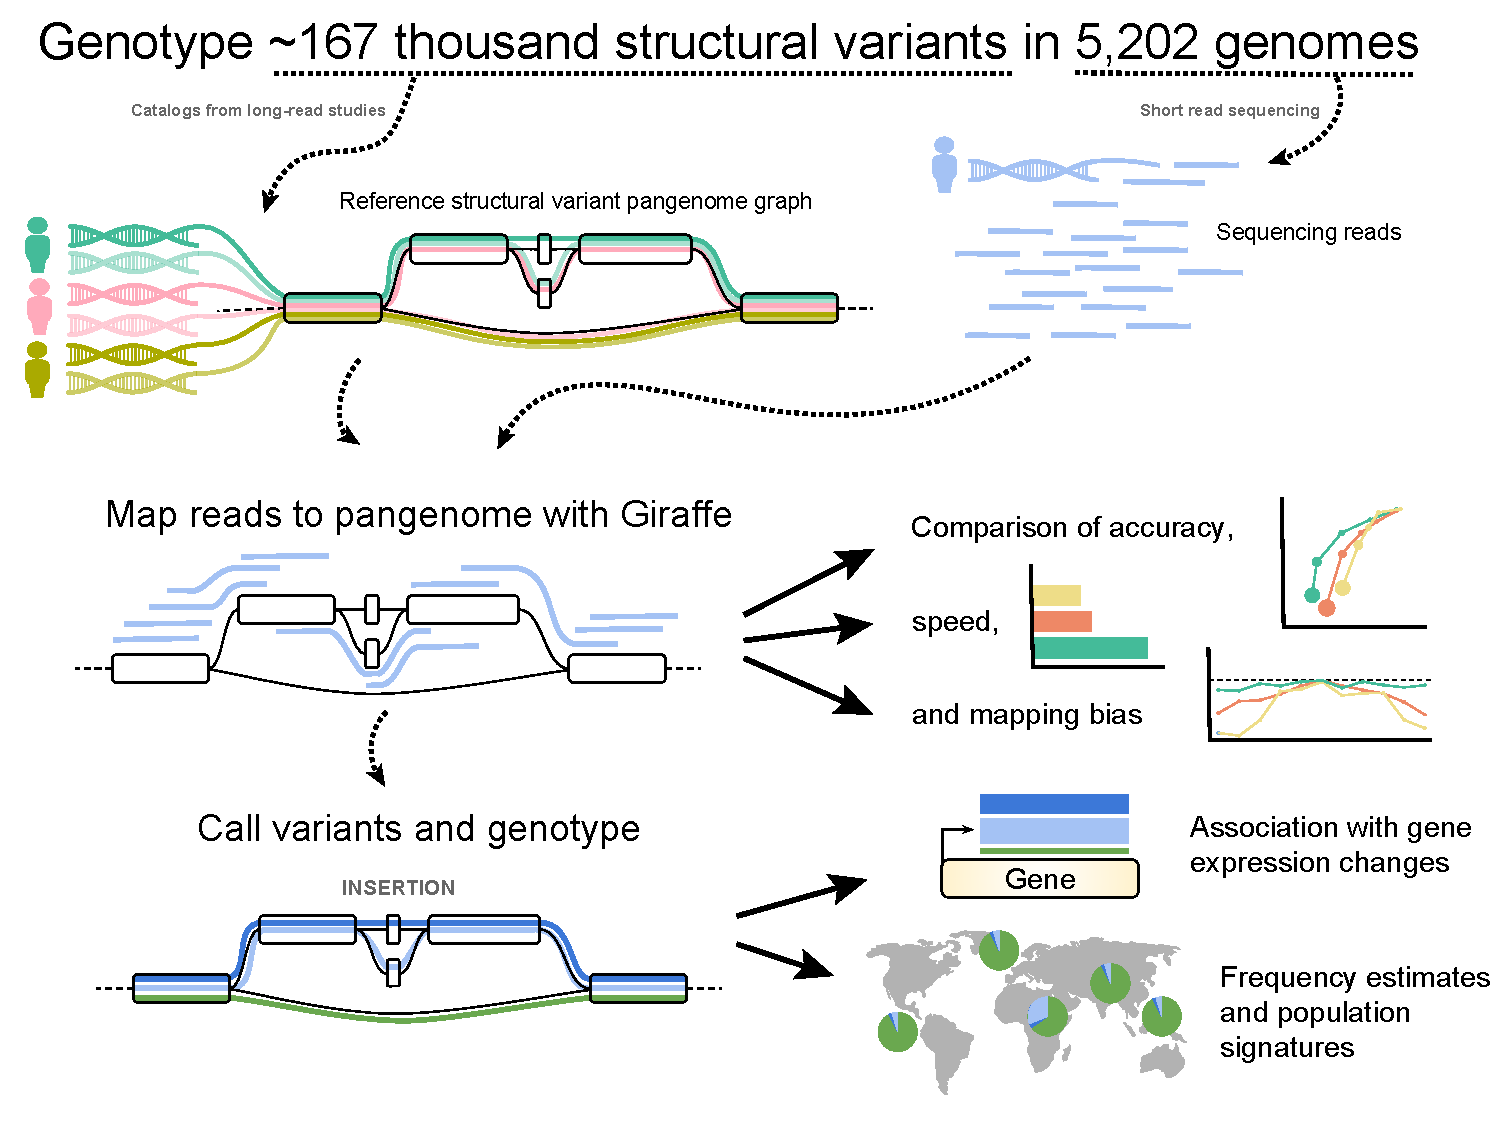
\includegraphics[width=.8\linewidth]{aim2_summary.pdf}
    \caption[Overview of short read Giraffe experiments]{\textbf{Overview of the experiments} Variant calls from long read–based and large-scale sequencing studies were used to construct pangenome reference graphs (top). Giraffe (and competing mappers) mapped reads to the graph or to linear references, and mapping accuracy, allele coverage balance, and speed were evaluated (middle). Then, mapped reads were used for variant calling, and variant call accuracy was evaluated (bottom). Structural variant calls were analyzed alongside expression data to identify eQTLs and population frequency estimates.}
    \label{fig:aim2_summary}
\end{figure}

\section{Introduction}
The field of genomics almost exclusively uses a single reference genome assembly as an archetype of a human genome.
Reliance on comparing with the sequences within the reference assembly has created a pervasive bias toward the alleles it contains.
This reference allele bias occurs because nonreference alleles are naturally harder to identify when mapping DNA sequencing data to the reference sequences.
Reference allele bias is particularly acute for structural variations (SVs), which are complex alleles involving 50 or more nucleotides of divergent sequence.
SVs affect millions of bases within each human genome.
Because of reference allele bias, SVs are much more poorly characterized than single-nucleotide variants (SNVs) and short insertions and deletions (collectively termed indels)\cite{zook_robust_2020,mahmoud_structural_2019}.
Similarly, characterizing genetic variation in highly polymorphic and repetitive sequences has proven challenging \cite{ebler_genotyping_2017}.

Recent releases of the reference human genome assembly attempted to address these issues by adding additional sequences.
These alternate sequences represent diversity in localized regions of the genome \cite{church_modernizing_2011}.
However, to date, these limited additions have not found widespread use. By contrast, pangenomes encode information about many complete genome assemblies and their homologies (the sequences that are shared between genomes by virtue of descending from a common ancestral sequence).
Pangenomes are emerging as a replacement for linear reference assemblies to help mitigate these problems \cite{noauthor_computational_2016,sherman_pan-genomics_2020,ballouz_is_2019}.
They can particularly improve genotyping of structural variants \cite{hickey_vgsv_2020}.

Pangenomes are frequently formulated as sequence graphs \cite{eizenga_pangenome_2020}—mathematical graphs that represent the homology relationships between multiple sequences.
Several algorithms have been developed for mapping sequences to sequence graphs.
None has yet made mapping the short sequencing reads from widely used DNA sequencers, such as those made by Illumina, to a structurally complex pangenome a practical option for large-scale applications.
The original VG-MAP algorithm \cite{garrison_vg_2018} maps to complex sequence graphs that contain cycles produced by duplications and complex genomic rearrangements \cite{garrison_vg_2018}.
However, VG-MAP is at least an order of magnitude slower than popular linear genome mappers that have comparable accuracy.
Given that mapping is frequently a bottleneck in genome analysis, the cost of VG-MAP has proven prohibitive. Other pangenome mappers have different capabilities and limitations.
Some are faster but are limited to acyclic graphs that contain variation at relatively low density \cite{kim_hisat2_2019}, and some can map to arbitrary sequence graphs but are designed for long reads \cite{rautiainen_graphaligner_2020}. Other tools are not open source and are thus unavailable for general testing and customization \cite{sevenbridges_2019,illumina_dragen_2019}, and some additionally cannot run on commodity computing environments \cite{illumina_dragen_2019}.

\section{Results}
\subsection{Giraffe: Fast, haplotype-aware pangenome mapping}
When a sequence graph reference \cite{noauthor_computational_2016} (Figure \ref{fig:aim2_supplement_graph-example}) is substituted for the traditional linear reference (Figure \ref{fig:aim2_fig1} A), it can reduce reference allele bias by including more alleles \cite{garrison_vg_2018}. 
However, it also expands the size of the alignment search space from a few linear chromosome strings to a combinatorially large number of paths in the graph.
This has made our previous graph mappers slower than linear mappers \cite{garrison_vg_2018}.
Giraffe solves this problem by considering the paths that are observed in individuals’ genomes: the reference haplotypes.
We use the two haplotypes (one from each parent) that each individual has in their genome and trace them as paths through the sequence graph.
The graph describes which positions in the haplotypes are equivalent, whereas the haplotypes describe the subset of the possible paths in the graph to consider.
Giraffe uses a graph Burrows-Wheeler transform (GBWT) index \cite{siren_indexes_2020} to store and query a graph’s haplotypes efficiently.

Giraffe’s strategy of aligning to haplotype paths has two key benefits.
First, it prioritizes alignments that are consistent with known sequences, thereby avoiding combinations of alleles that are biologically unlikely.
Second, it reduces the size of the problem by limiting the sequence space to which the reads could be aligned.
This deals effectively with complex graph regions where most paths represent rare or nonexistent sequences.

We designed Giraffe to minimize the amount of gapped alignment that is performed.
Computing gapped alignments, in which sequences are allowed to gain or lose bases relative to each other, is much more expensive than gapless alignment because it requires pairwise dynamic programming algorithms.
Most Illumina sequencing errors are substitutions \cite{schirmer2016illumina}, and common true indels relative to the traditional linear reference should already be present in the haplotypes; therefore, almost all reads will have a gapless alignment to some stored haplotype.
Hence, we try to align each read without gaps before resorting to dynamic programming.

Giraffe follows the common seed-and-extend approach used by most existing mappers (Section \ref{subsec:aim2:giraffe-methods}.
In this framework, short seed matches between a sequencing read and a genomic reference are found with minimal work, and then only good seeds are extended into mappings of the entire read \cite{langmead_bowtie2_2012,li_bwa_mem_2013,li_minimap2_2018}.
A visual overview of Giraffe’s operation is given in (Figure \ref{fig:aim2_fig1}, B to F).
The Giraffe algorithm uses several heuristics for prioritizing alignments.
These heuristics are configurable, and we present two presets: default Giraffe (written as just “Giraffe”) balances speed and accuracy, and fast Giraffe optimizes for speed at the expense of some accuracy.
\begin{figure}
    \centering
    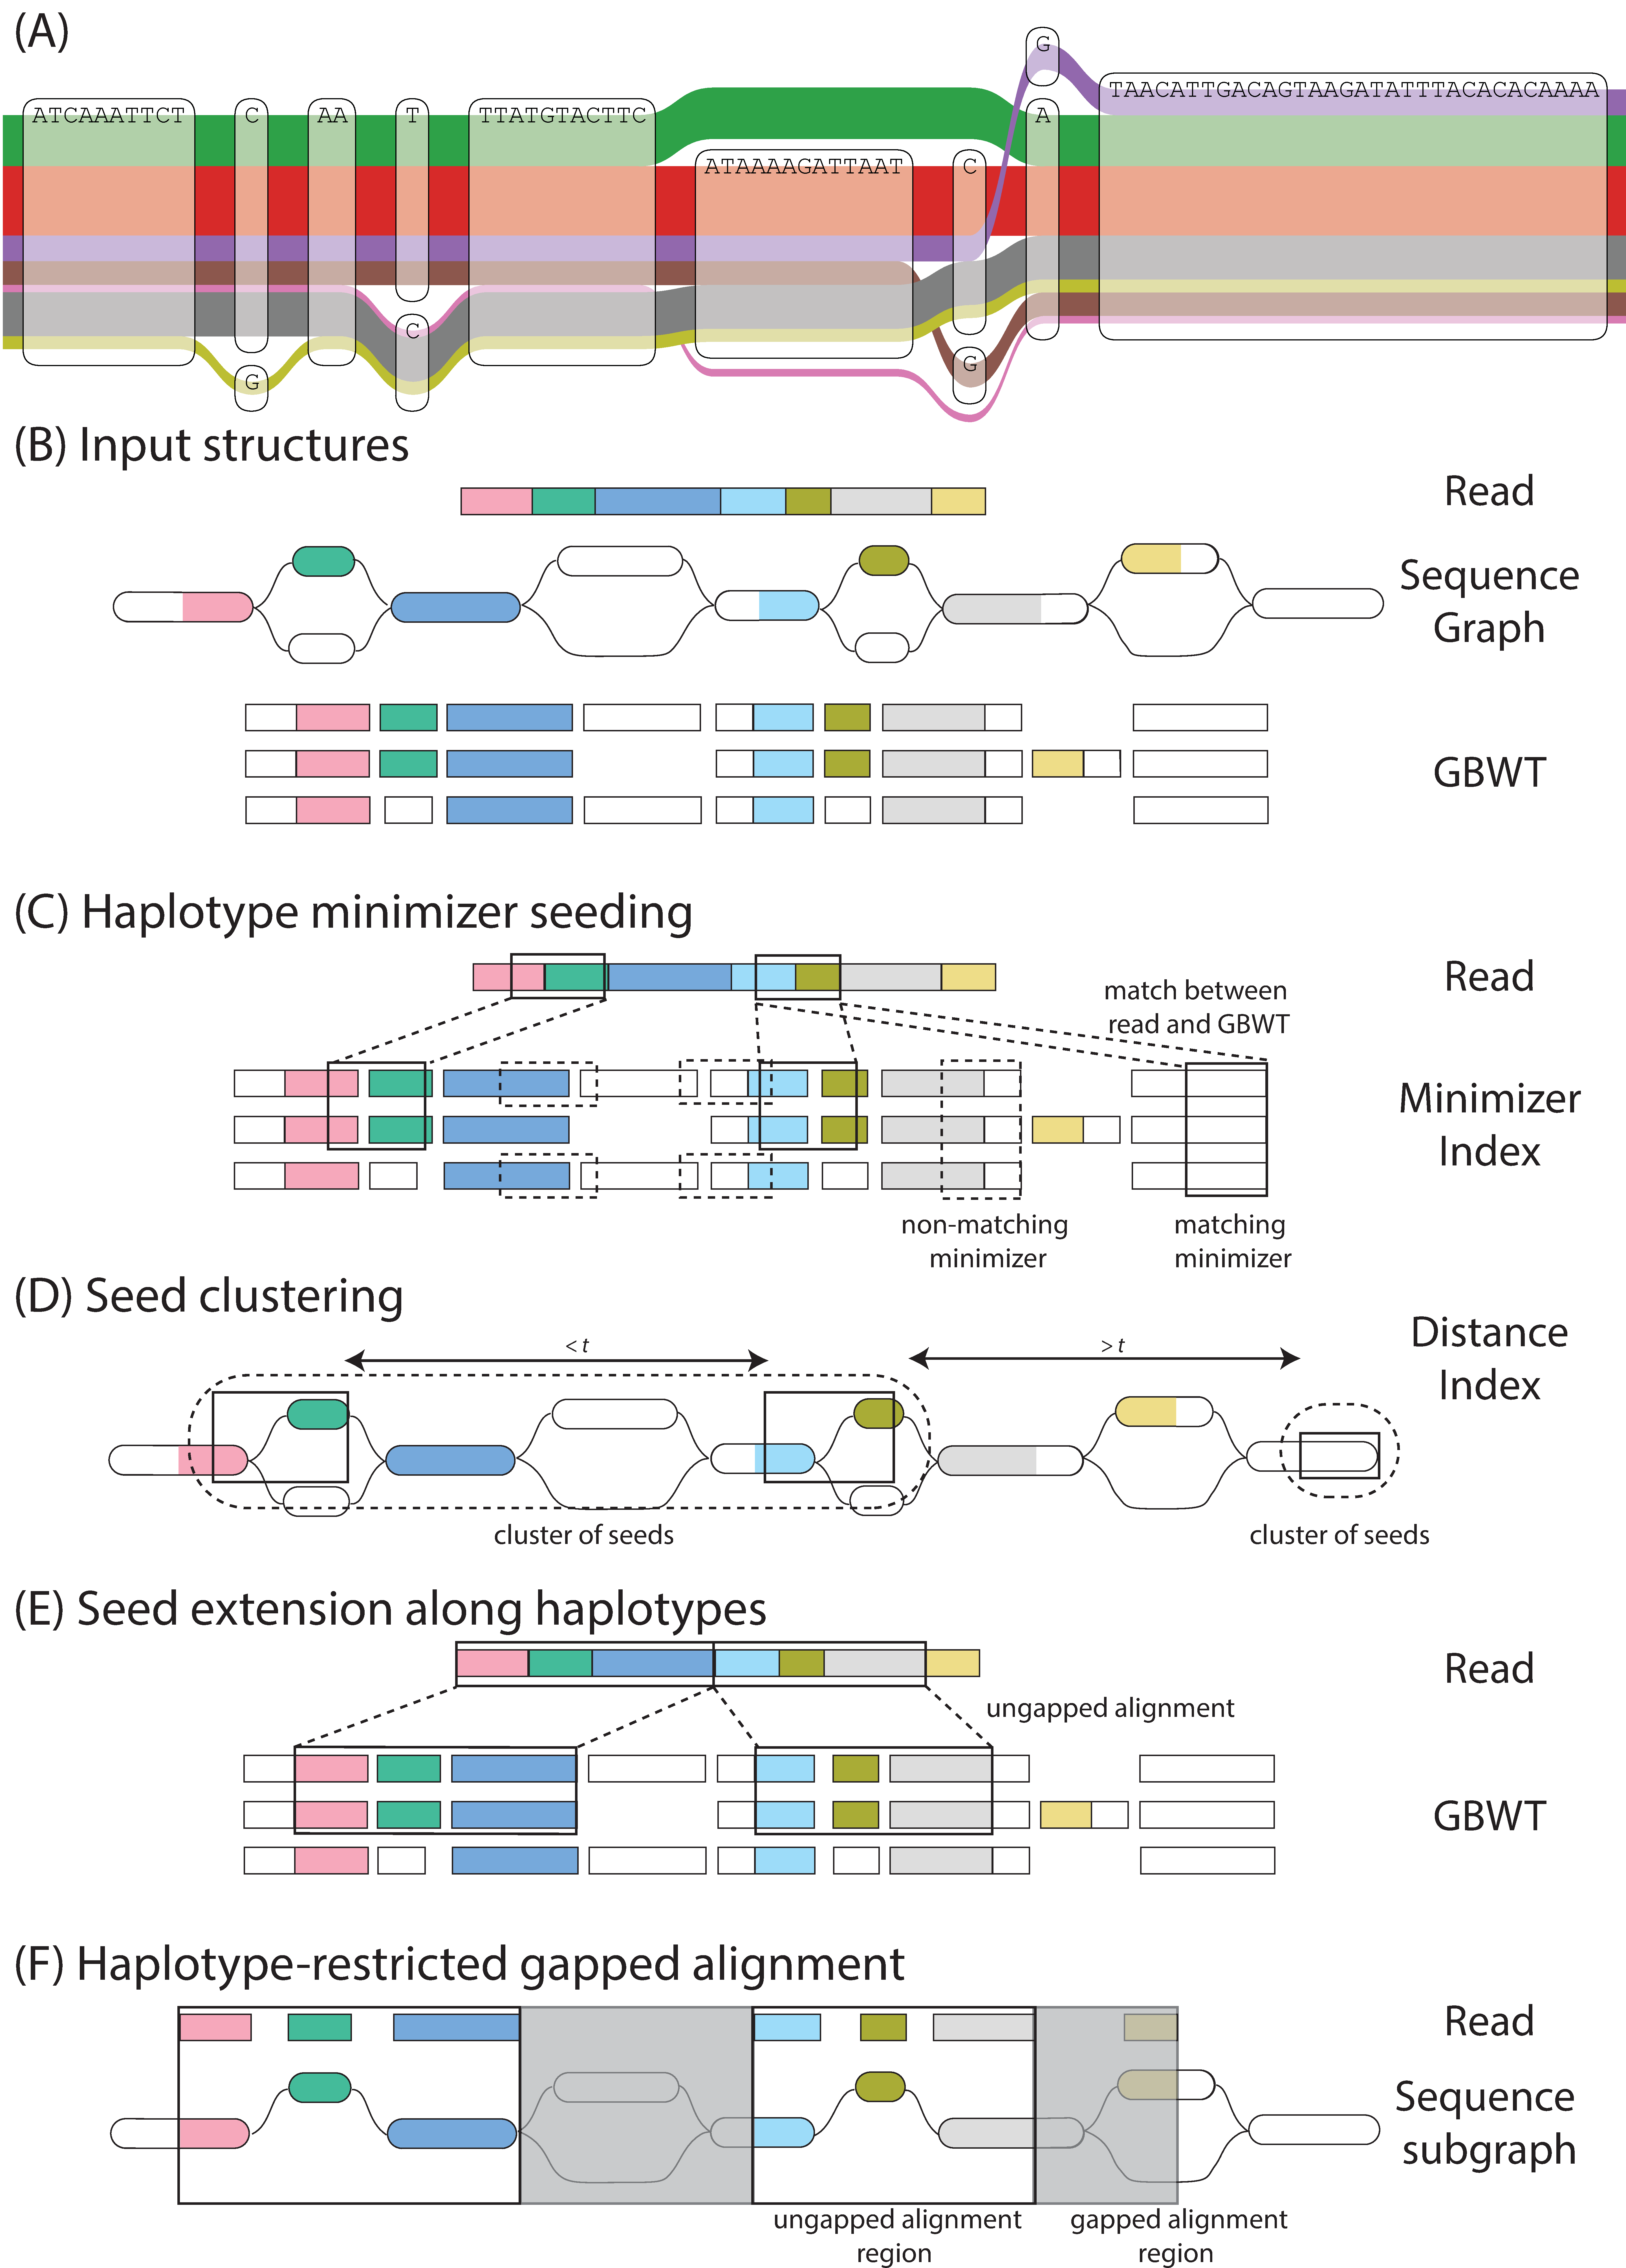
\includegraphics[width=.5\linewidth]{aim2_fig1.pdf}
    \caption[Short read giraffe algorithm]{\textbf{Haplotype mapping.} (A) A region of the CASP12 gene in the 1000GP graph, illustrating complex local variation. The observed haplotypes (the colored ribbons of width log-proportional to population frequency) represent only a subset of the possible paths through the graph. (B to F) An overview of Giraffe. Input structures are shown in (B): Giraffe takes as input each read to map, the sequence graph reference to map against, and the GBWT of known haplotypes to restrict to. The input read is represented as a series of colored rectangles. The haplotype sequences in the GBWT are similarly represented as series of rectangles, split according to the nodes they correspond to in the sequence graph. Nodes in the sequence graph and haplotypes in the GBWT are colored according to homology with the read. Haplotype minimizer seeding is shown in (C): Seeds are identified using an index of minimizers (subsets of sequences of specified length k)\cite{Roberts2004} over the sequences of all the GBWT haplotypes. A matching minimizer between the read and the GBWT haplotypes constitutes a seed. The minimizers (black boxes) in the read are enumerated and the matching minimizers in the haplotypes are identified using the minimizer index. Seed clustering is shown in (D): Minimizer instances in the graph are clustered by the minimum graph distance (t, measured in nucleotides) between them \cite{chang_distance_2020}. Seed extension along haplotypes is shown in (E): Minimizers in high-scoring clusters are extended linearly to form maximal gapless local alignments. Haplotype-restricted gapped alignment is shown in (F): Giraffe is designed on the assumption that for most reads, it will be possible to gaplessly extend seed alignments all the way to the ends of the read, allowing the algorithm to stop at the previous step. However, any remaining gaps in the alignment between read and graph are resolved by gapped alignment in this final step.}
    \label{fig:aim2_fig1}
\end{figure}

\subsection{Pangenome references for evaluation}
To evaluate Giraffe, we built two human genome reference graphs based on the GRCh38 reference assembly.
One (the 1000GP graph) contained mostly small [$<50$ base pairs (bp)] variants from the 1000 Genomes Project \cite{1000gp_2015}.
The other (the HGSVC graph) contained entirely SVs ($\geq$50 bp) from the Human Genome Structural Variant Consortium \cite{chaisson_sv_2019}.
The 1000GP graph contained data from 2503 individuals, with one (NA19239) held out for benchmarking.
It was built from 76,749,431 SNVs; 3,177,111 small indels ($<50$ bp); and 181 larger SVs ($\geq$50 bp).
The HGSVC graph contained data from three individuals sequenced with long reads: HG00514, HG00733, and NA19240.
The HGSVC graph contained 78,106 larger SVs ($\leq$50 bp). Both graphs are available for reuse (see Data and materials availability in the Acknowledgments).

\subsection{Giraffe and VG-MAP map accurately to human pangenomes}
We evaluated Giraffe for mapping human data by simulating paired-end reads for two individuals (Section \ref{subsec:aim2:readsim}): NA19240, who has available genotypes for the HGSVC variants \cite{chaisson_sv_2019}, and NA19239, who has available genotypes for the 1000GP variants \cite{1000gp_2015}.
Simulated read sets were mapped using Giraffe and competing tools (Section \ref{subsec:aim2:readmapping}).
We examined the accuracy of single- and paired-end mapping (Figure \ref{fig:aim2_fig2}).
We looked at a variety of input read sets and evaluated the calibration of reported mapping quality, which is a standard measure of mapping uncertainty (Figures.\ref{fig:aim2_supplement_novaseq_rocs},\ref{fig:aim2_supplement_hiseqxten_rocs},\ref{fig:aim2_supplement_hiseq2500_rocs},\ref{fig:aim2_supplement_novaseq6000_qq},\ref{fig:aim2_supplement_hiseqxten_qq},\ref{fig:aim2_supplement_hiseq2500_qq} and Tables \ref{tab:mapping_accuracy_1kg_novaseq6000},\ref{tab:mapping_accuracy_1kg_hiseqxten},\ref{tab:mapping_accuracy_1kg_hiseq2500},\ref{tab:mapping_accuracy_hgsvc_novaseq6000},\ref{tab:mapping_accuracy_hgsvc_hiseqxten},\ref{tab:mapping_accuracy_hgsvc_hiseq2500}).
Relative to other tools, at the highest reported mapping quality, VG-MAP and default Giraffe consistently have either higher precision or higher recall across all simulated read technologies and graphs.
Their performance is generally similar.
Relative to the linear mappers, the Giraffe and VG-MAP lead is larger for the HGSVC graph (Figure \ref{fig:aim2_fig2}, C and D) than for the 1000GP graph (Figure \ref{fig:aim2_fig2}, A and B).
This suggests that the gains from using a genome graph are higher when the graph facilitates alignment of genomic sequences from the sample that differ greatly from the linear reference.
\begin{figure}
    \centering
    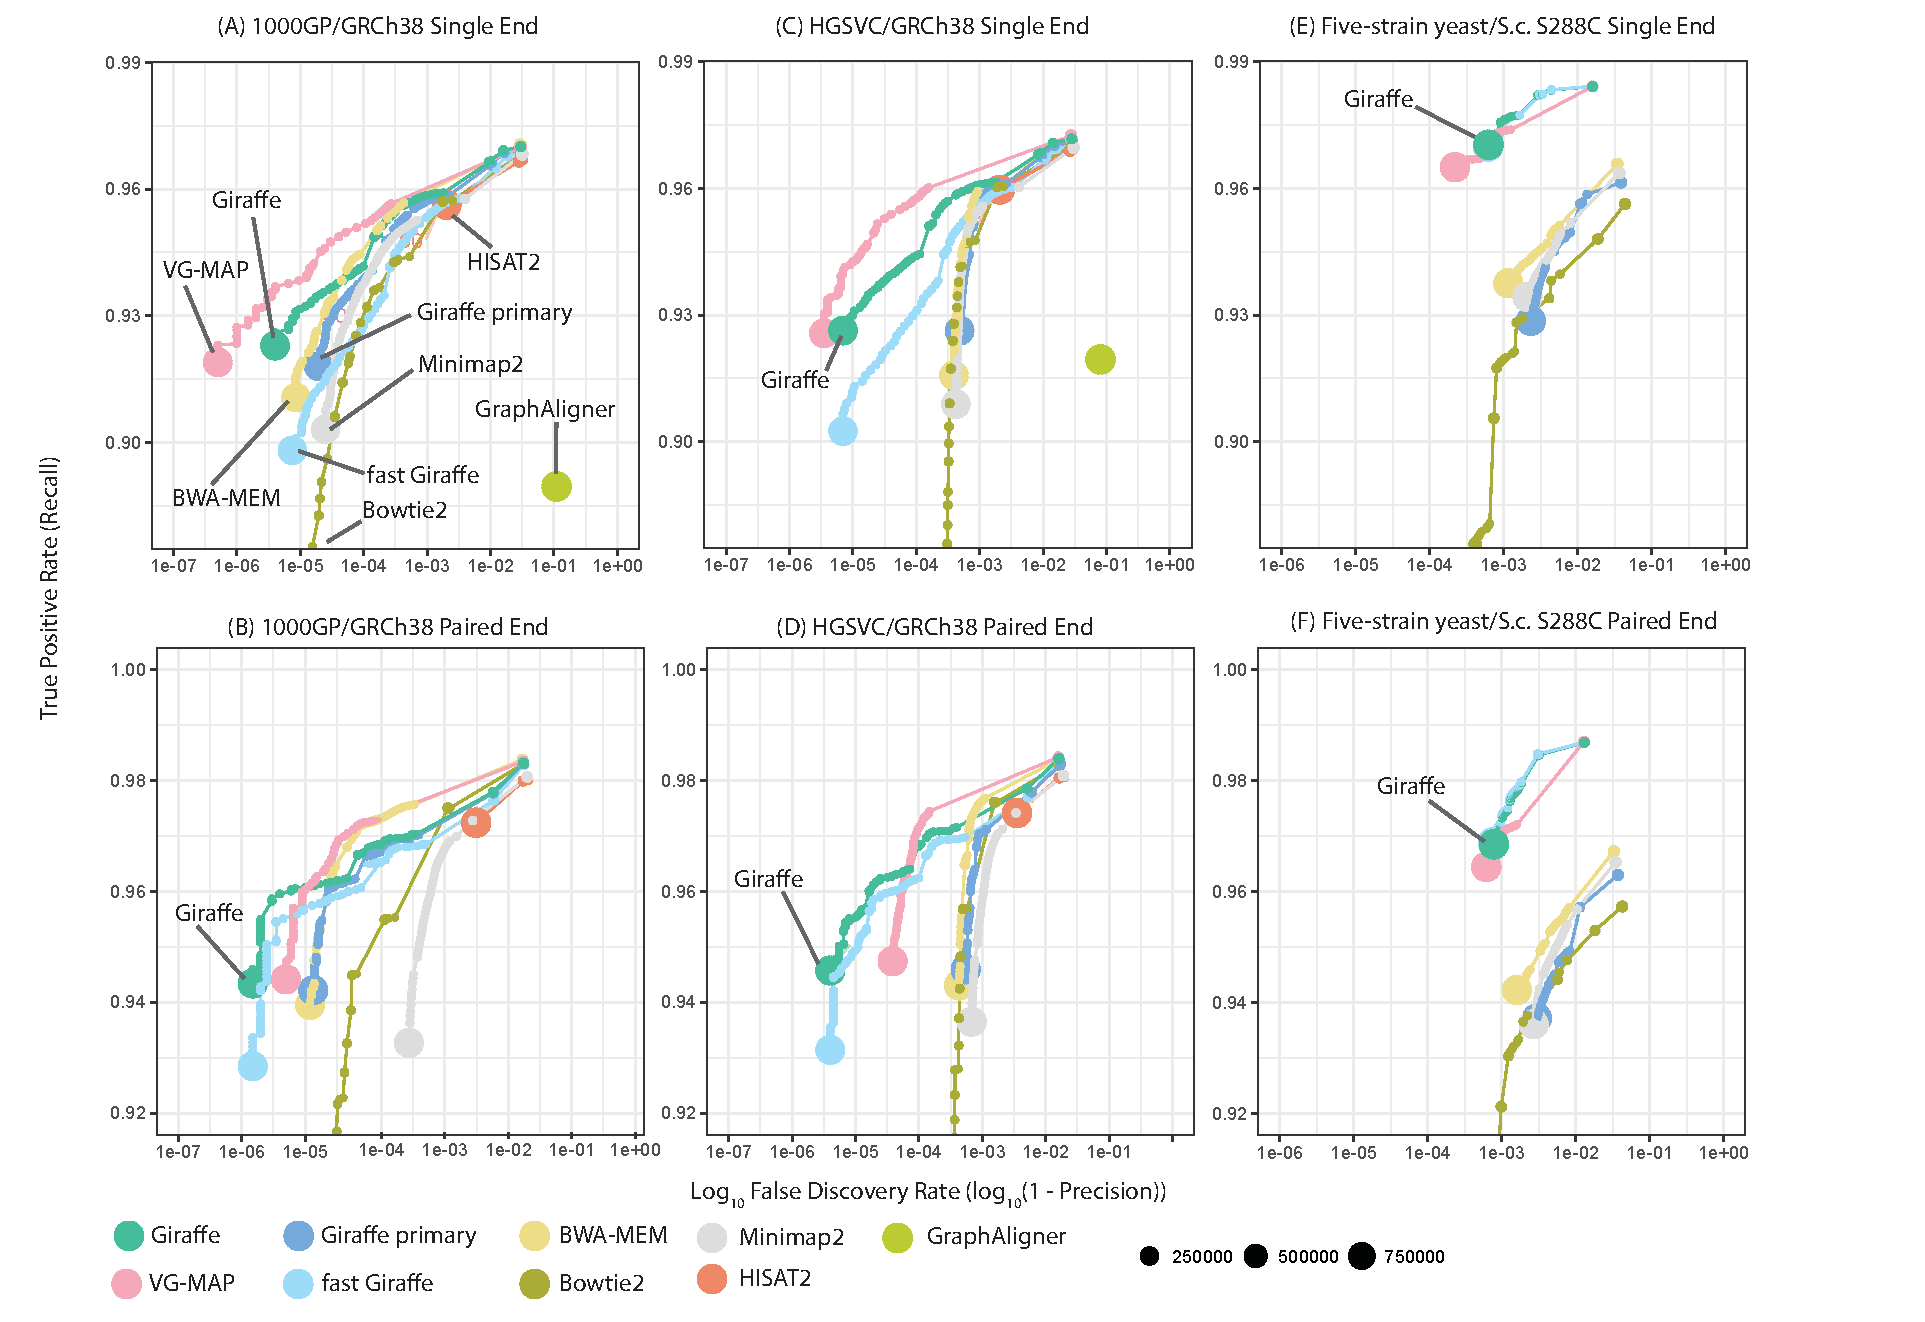
\includegraphics[width=\linewidth]{aim2_fig2.pdf}
    \caption[Short read simulated read mapping]{\textbf{Simulated read mapping} (A to F) Each panel shows recall versus false discovery rate (or 1 minus precision) for a simulated read-mapping experiment, comparing Giraffe with linear genome mappers (BWA-MEM, Bowtie2, and Minimap2) and other genome graph mappers (VG-MAP, GraphAligner, and HISAT2). Reads were simulated to match $\sim150$-bp Illumina NovaSeq (for human) or HiSeq 2500 (for yeast) reads, either as single-end reads [(A) to (C)] or as paired-end reads [(D) to (F)] (Section \ref{subsec:aim2:readsim}). Results for each mapper are shown stratified by reported read-mapping quality; the size of each point represents the log-scaled number of reads with the corresponding mapping quality. Three different mapping scenarios are assessed: [(A) and (D)] Comparing mapping to a graph derived from the 1000GP data to mapping to the linear reference genome assembly upon which it is based (GRCh38); [(B) and (E)] comparing mapping to a graph containing larger structural variants from the HGSVC project to mapping to the GRCh38 assembly upon which it is based; and [(C) and (F)] comparing mapping to a multiple sequence alignment–based yeast graph to mapping to the single S.c. S288C linear reference, for reads from the DBVPG6044 strain. For mapping with Giraffe, we used the full GBWT that contains six haplotypes to map to the HGSVC graph and the 64-haplotype sampled GBWT to map to the 1000GP graph. “Giraffe primary” represents mapping with Giraffe to the linear reference.}
    \label{fig:aim2_fig2}
\end{figure}

\subsection{Haplotype sampling improves read mapping}
Having rare variants or errors in the graph and haplotypes may reduce mapping accuracy by creating opportunities for false-positive mappings \cite{Pritt2018}.
Mapping reads to regions with many distinct local haplotypes can also be slow.
Additionally, Giraffe needs a mechanism to synthesize haplotypes for graph components where no haplotype variation is known.
To overcome these issues, Giraffe includes mechanisms for creating synthetic haplotype paths.
When real haplotypes are available, these synthetic haplotype paths represent local haplotype variation sampled according to haplotype frequency, and we call the result a sampled GBWT (Section~\ref{subsec:aim2:downsampling}).
When no haplotypes are available, we call the result a path cover GBWT.
In this case, the synthetic haplotypes represent random walks through the graph. We evaluated the effects of running our mapping evaluations with sampled and path cover GBWTs (Figure \ref{fig:aim2_supplement_haplotype_sampling} and Tables \ref{tab:mapping_accuracy_1000gp_sampled_gbwt} and \ref{tab:mapping_accuracy_hgsvc_cover_gbwt}; Section~\ref{subsec:aim2:downsamplingeval}).
The mapping benefit of sampling more haplotypes plateaued at 64 haplotypes for the 1000GP graph (which contains around 5000 haplotypes), with higher accuracy than that achieved by mapping to the full haplotype set.
We used the HGSVC graph (which contains just six haplotypes) for an experiment on generating path covers without known haplotypes.
Path covers alone did not outperform the full underlying haplotype set for the HGSVC graph but came close to matching its performance.
We selected the 64-haplotype sampled GBWT for the 1000GP graph and the full GBWT for the HGSVC graph as the best-performing GBWTs, which we use in the rest of the analysis.

\subsection{Giraffe improves pangenome mapping speed}
We measured the runtime (Figure \ref{fig:aim2_fig3}, A and B) and memory usage (Figure \ref{fig:aim2_fig3}, C and D) of Giraffe and competing tools when mapping real reads (Section \ref{subsec:aim2:srgiraffe_speed}).
Giraffe was more than an order of magnitude faster than VG-MAP in all conditions.
It was also faster at aligning to human graphs than Bowtie2 or BWA-MEM were at aligning to the corresponding linear reference.
For the 1000GP graph, using the 64-haplotype sampled GBWT for mapping instead of the full $\sim$5000-haplotype GBWT was much faster in every case.
HISAT2 and fast Giraffe were both about equally fast and were both faster than all other mappers.

Because of the in-memory indexes it uses, Giraffe’s memory consumption is higher than the other mappers, except for GraphAligner.
However, it can map to the 1000GP graph with the full GBWT in $\sim$80 gigabytes (GB) of memory—an amount readily available on compute cluster nodes (Figure \ref{fig:aim2_fig3}, C and D).

\begin{figure}
    \centering
    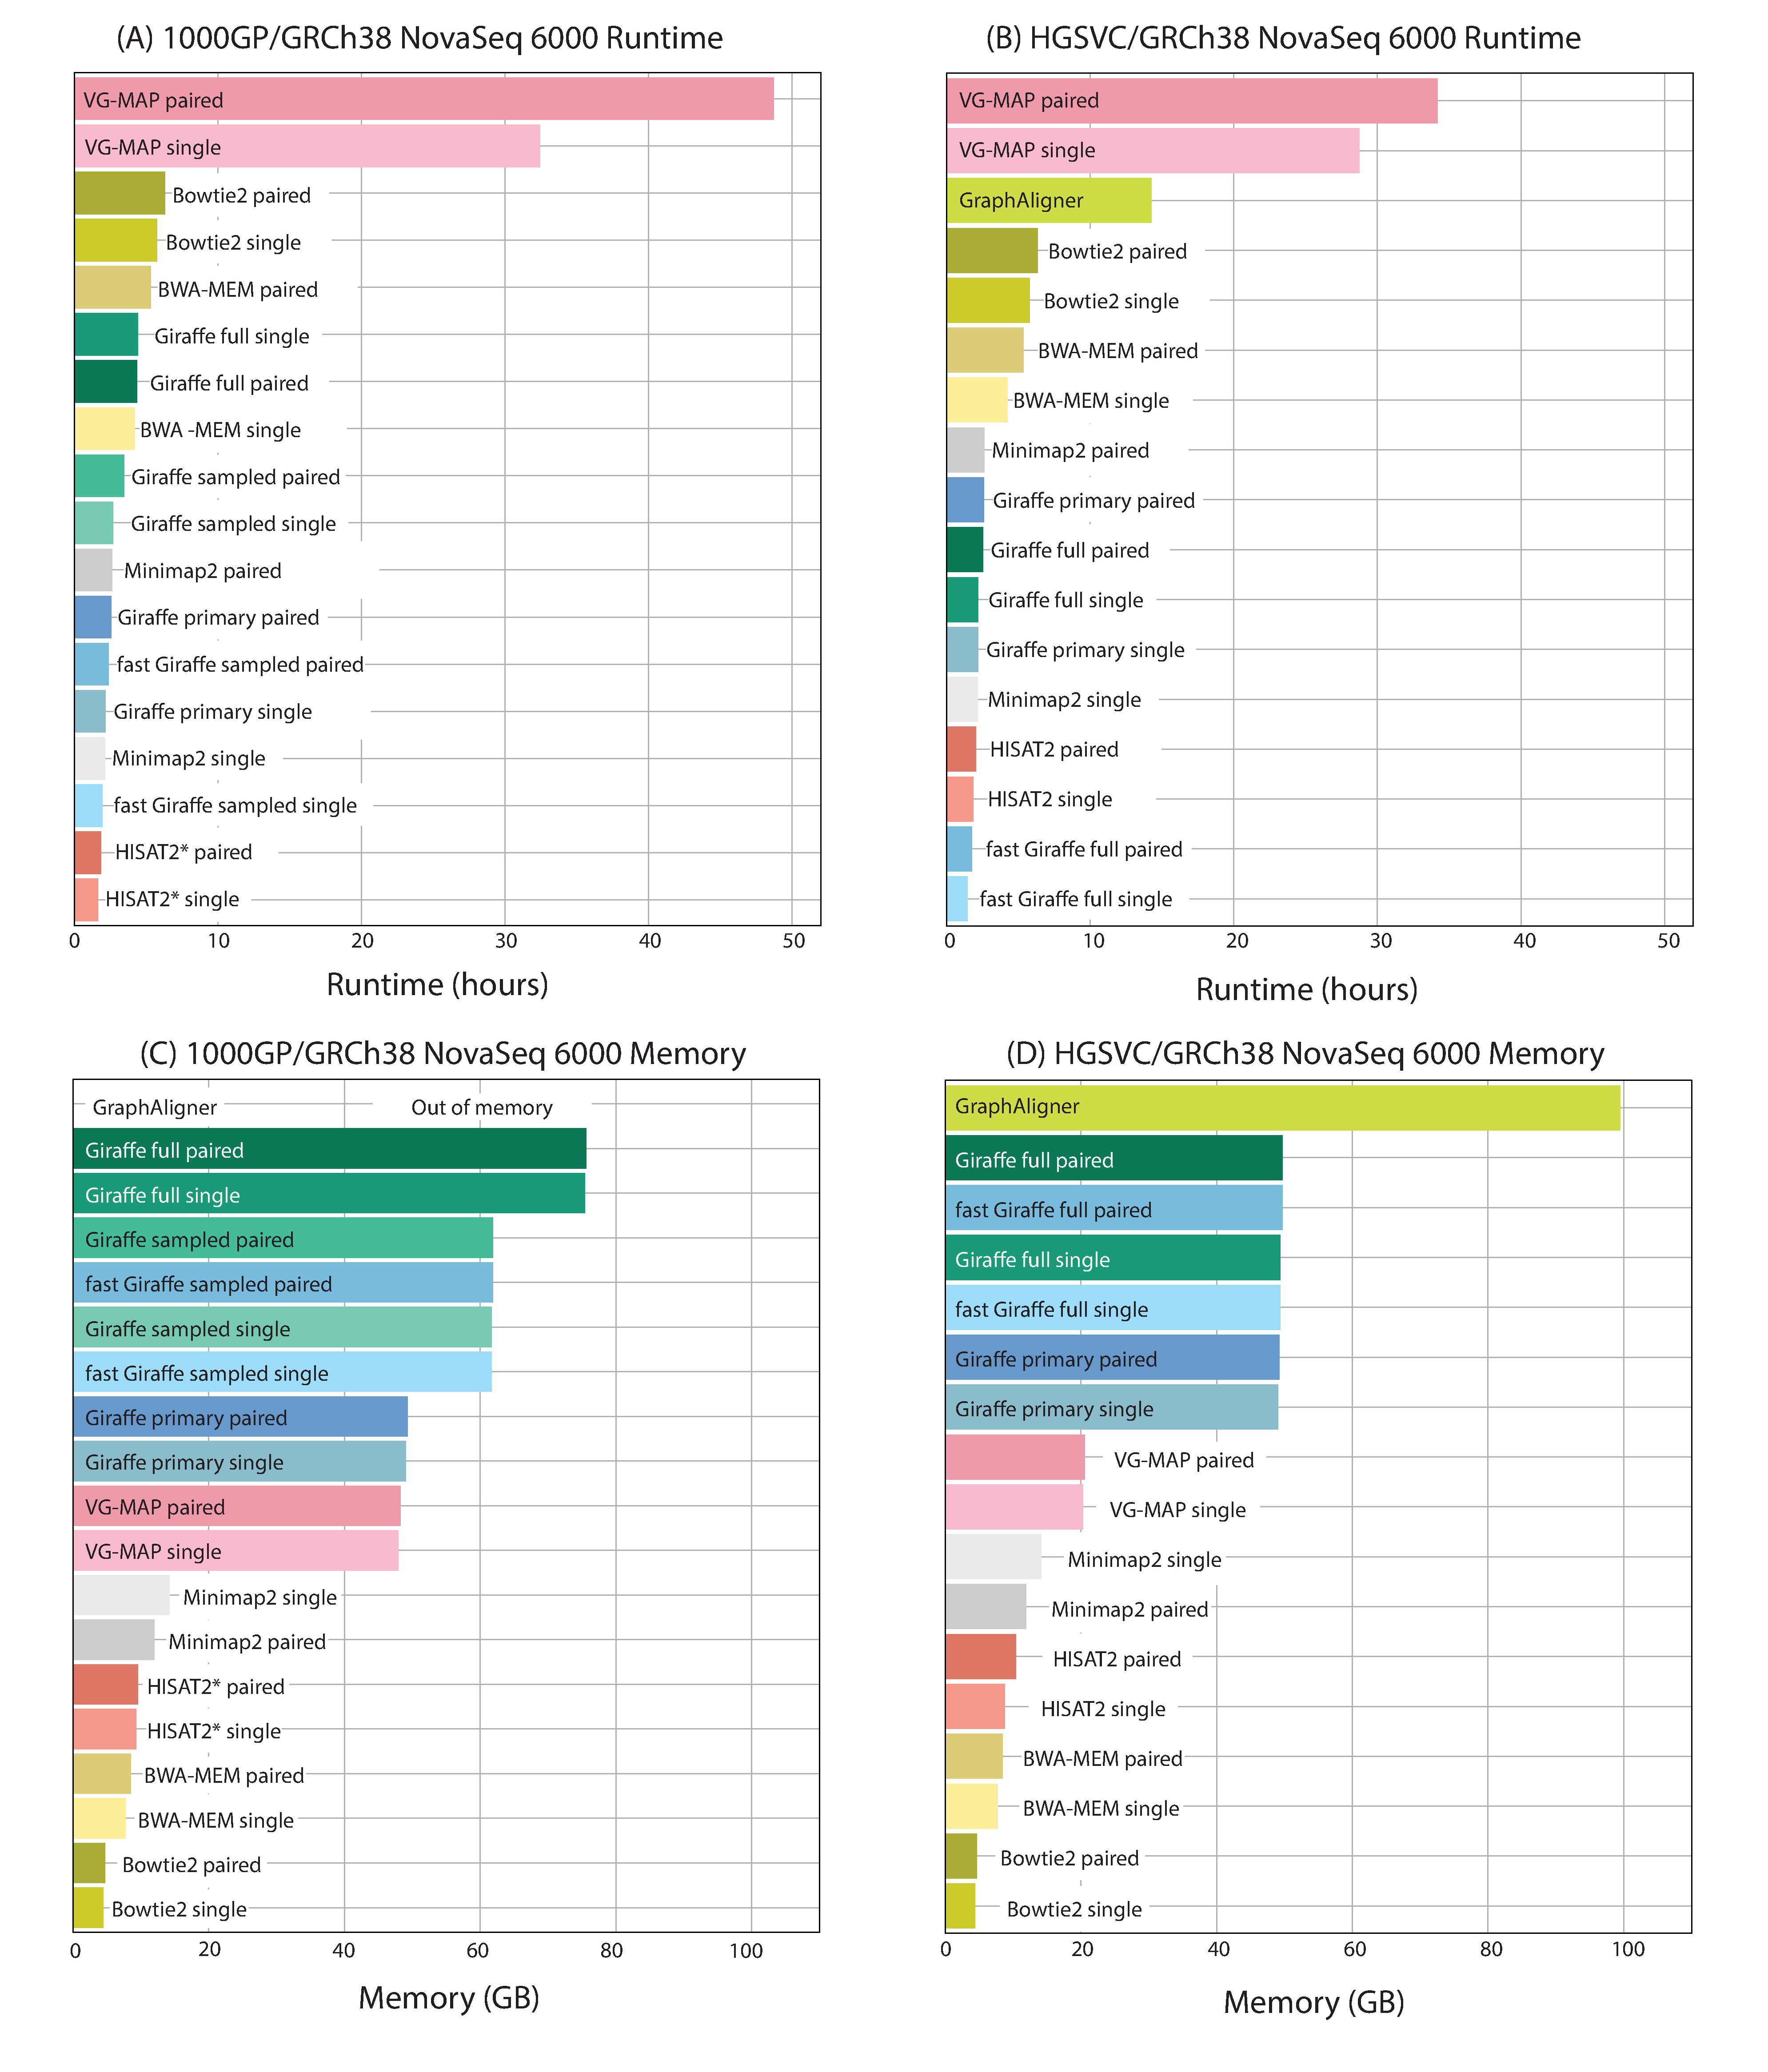
\includegraphics[width=.8\linewidth]{aim2_fig3.pdf}
    \caption[Short read runtime and memory usage]{\textbf{Runtime and memory usage} (A to D) Total runtime [(A) and (B)] and peak memory use [(C) and (D)] for mapping $\sim$600 million NovaSeq 6000 reads using 16 threads. Reads were mapped [(A) and (C)] to the 1000GP derived graph or (for linear mappers) the GRCH38 assembly and [(B) and (D)] to the HGSVC graph or GRCh38 reference, respectively. For HISAT2*, results are shown for the subset 1000GP graph. “Giraffe full” refers to mapping using the full GBWT of all haplotypes. “Giraffe sampled” refers to mapping using the 64-haplotype sampled GBWT.}
    \label{fig:aim2_fig3}
\end{figure}

\subsection{Giraffe reduces allele mapping bias}
We assessed Giraffe’s reference bias (Section \ref{subsec:aim2:srgiraffe_allelebias}).
We expected Giraffe to be able to use the extra variation information contained in the graph reference to achieve a lower level of bias than a linear mapper.
For variants that were heterozygous in NA19239, we found the fraction of reads supporting alternate versus reference alleles at each indel length (Figure \ref{fig:aim2_fig4} A).
Giraffe and VG-MAP both show less bias toward the reference allele than a linear mapper, and this difference becomes more pronounced as indel length increases, particularly for larger insertions.

\begin{figure}
    \centering
    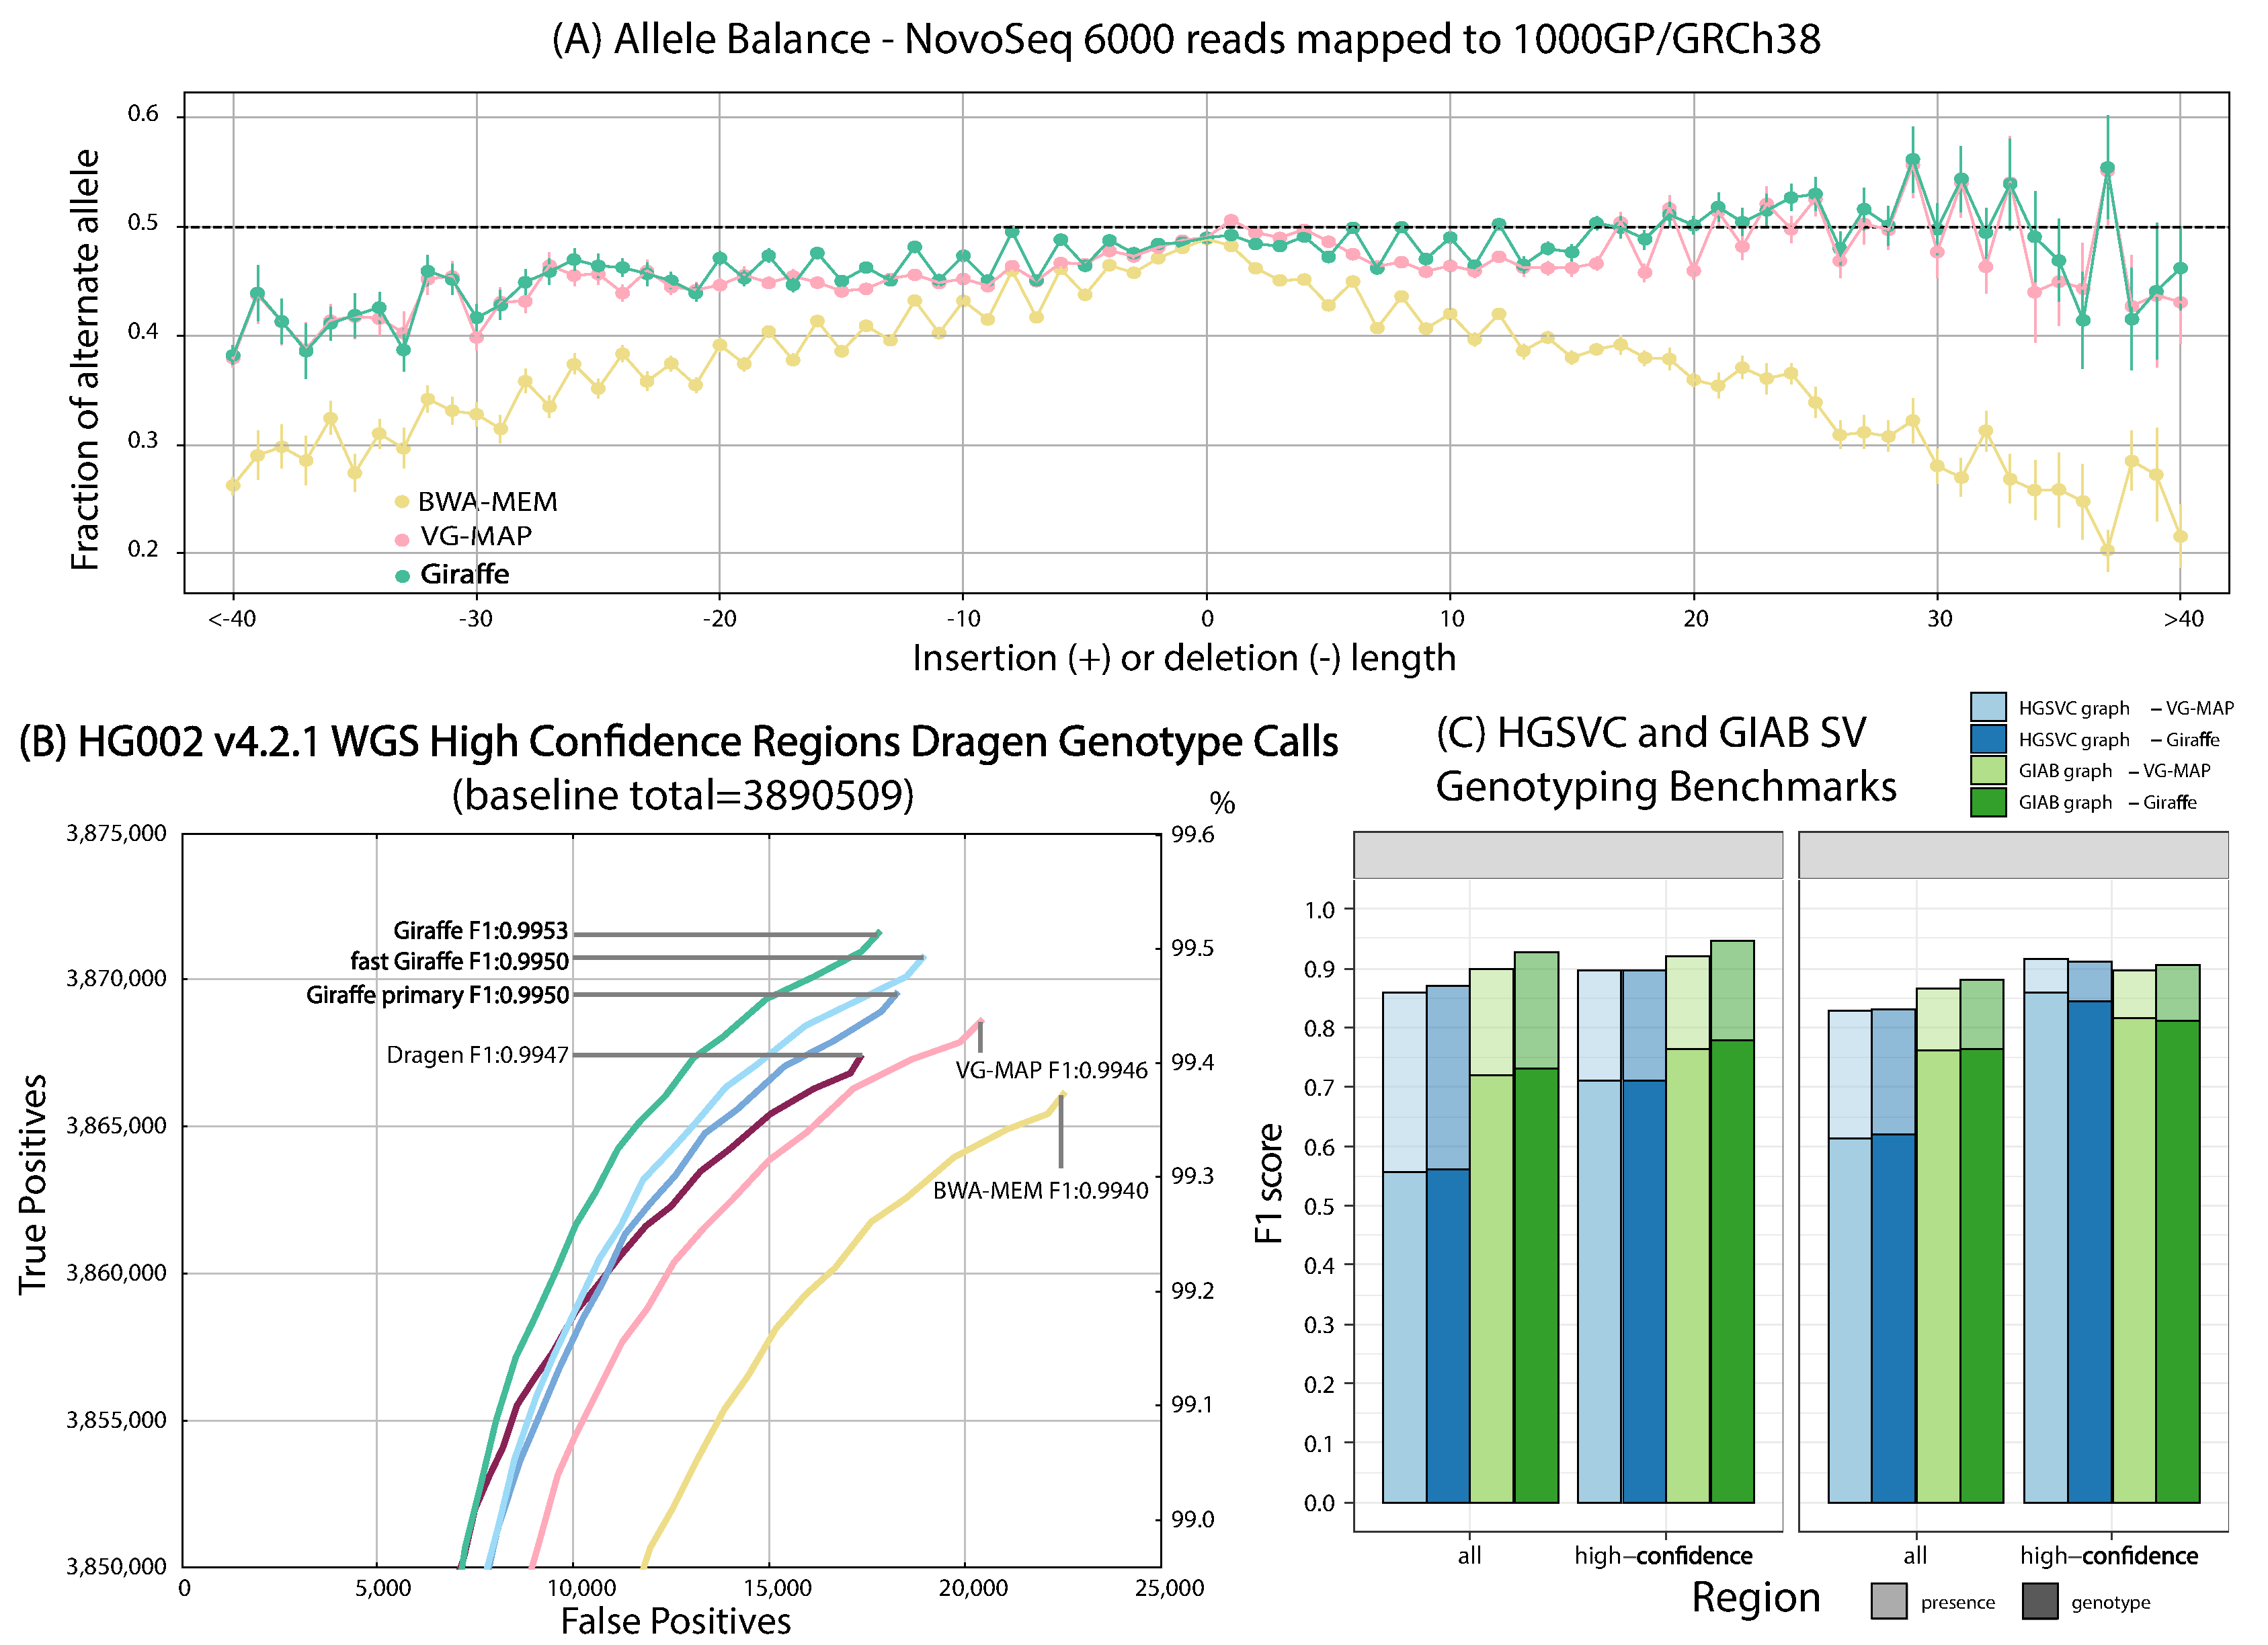
\includegraphics[width=\linewidth]{aim2_fig4.pdf}
    \caption[Evaluating Giraffe for genotyping with short reads]{\textbf{Evaluating Giraffe for genotyping.} (A) The fraction of alternate alleles in reads detected for heterozygous variants in NA19239. Reads were mapped to the 1000GP graph with Giraffe and VG-MAP and to GRCh38 with BWA-MEM, and the fraction of reads supporting reference or alternate alleles was found for each indel length. (B) Assessing true-positive and false-positive genotypes made using the Dragen genotyper with mappings from Giraffe and other mappers. The line labeled Dragen represents the mapper included with the Dragen system itself. (C) Comparing Giraffe with VG-MAP for typing large insertions and deletions. “Presence” (lighter bars) evaluates the detection of SVs without regard to genotype; “genotype” (darker bars) requires the SV to be detected and its genotype to agree with the truth genotype. The y axis shows the F1 score. For the HGSVC benchmark, we define high-confidence regions as regions not overlapping simple repeats and segmental duplications. For the GIAB benchmark, we use the set high-confidence regions provided by GIAB.}
    \label{fig:aim2_fig4}
\end{figure}

\subsection{Giraffe genotyping outperforms best practices}
We used Illumina’s Dragen platform \cite{illumina_dragen_2019} to genotype SNVs and short indels using Giraffe mappings to the 1000GP graph, projected onto the linear reference assembly.
We compared these results with results using competing graph and linear reference mappers (Section \ref{subsec:aim2:dragen}).
No training or optimization was performed for any of the mappings other than those performed by default by Dragen itself. We evaluated the calls using the Genome in a Bottle (GIAB) v4.2.1 HG002 high-confidence variant-calling benchmark \cite{wagner_benchmarking_2020}.

Out of the examined pipelines, Giraffe mappings to the 1000GP graph produce the highest overall F1 score (harmonic mean of precision and recall) at 0.9953 (Figure \ref{fig:aim2_fig4}B and Tables \ref{tab:vcfeval_high_conf_2x150_hg002_grch38}, \ref{tab:happy_high_conf_2x150_hg002_grch38}).
Similar but uniformly higher results were found with higher-coverage, 250-bp reads (Figure \ref{fig:250bp_genotyping}, Tables \ref{tab:vcfeval_high_conf_2x250_hg002_grch38}, \ref{tab:happy_high_conf_2x250_hg002_grch38}).
Although one would expect longer reads and higher coverage to produce better variant calls, with all else being equal, Giraffe has a slightly higher F1 score with the 150-bp read set (0.9953) than BWA-MEM with the higher coverage 250-bp read set (0.9952).
Restricting comparison only to confident regions that overlap variant calls from the 1000GP variants used in graph construction, Giraffe has the highest F1 score at 0.9995 relative to the other methods (Table~\ref*{tab:vcfeval_high_conf_1000GP_only_2x150_hg002_grch38} and Figure~\ref*{fig:150bp_genotyping_1000GP_only}).
Perhaps surprisingly, Giraffe maintains the highest F1 score (0.9528) when performing the converse analysis, restricting the comparison to confident regions that do not overlap 1000GP variant calls (Table~\ref*{tab:vcfeval_high_conf_1000GP_excluded_2x150_hg002_grch38} and Figure~\ref*{fig:150bp_genotyping_1000GP_excluded}).

DeepVariant is a highly accurate genotyping tool that requires training \cite{deep_variant_2018}.
We trained DeepVariant to use Giraffe mappings and evaluated it on the held-out sample HG003 (see \ref{subsec:aim2:genotyping-accuracy-methods}).
We compared it with the Dragen pipelines tested and DeepVariant using BWA-MEM with the BWA-MEM trained model that the developers provide.
The Giraffe-DeepVariant pipeline (F1: 0.9965) outperforms all other tested pipelines (Tables~\ref*{tab:deepvariant_vcfeval_high_conf_2x150_50x_hg003_grch38}, \ref*{tab:deepvariant_happy_high_conf_2x150_50x_hg003_grch38} and Figure~\ref*{fig:trained_deepvariant_genotyping}).

Previously, when we used VG-MAP to map reads to SV pangenomes, we found it to perform better than other methods for SV genotyping \cite{hickey_vgsv_2020}.
We replicated that evaluation on the HGSVC and GIAB datasets \cite{zook_robust_2020,chaisson_sv_2019} to confirm that the quality of the SV genotypes from Giraffe was competitive (Section \ref{subsec:aim2:svgenotyping}).
We observed similar SV genotyping accuracy across SV types, genomic regions, and datasets (Figure \ref{fig:aim2_fig4} C). Of note, GraphTyper \cite{eggertsson2019}, which was published after our earlier benchmarking analysis \cite{hickey_vgsv_2020}, was also compared with vg as a variant caller but showed lower genotyping performance across SV types, genomic regions, and datasets  (Figure \ref{fig:graphtyper_eval}).

\subsection{Giraffe generalizes beyond human}
We assessed Giraffe’s performance mapping to a yeast pangenome for five strains of the Saccharomyces cerevisiae and Saccharomyces paradoxus yeasts (Section \ref{subsec:aim2:yeast-methods}).
This graph was substantially different from the human graphs.
It proved challenging because it contains the cycles and duplications typical of graphs generated from genome-wide alignments of more divergent sequences.
Using a graph decomposition technique \cite{paten_superbubbles_2018}, we find it contains 1,459,769 variant sites, four times the density of variation in the 1000GP graph.
Ninety of these sites are complex, meaning that they are not directed, not acyclic, or not free of internal source and sink nodes.

Mapping accuracy results for reads from the held-out S. cerevisiae DBVPG6044 strain are displayed in Figure \ref{fig:aim2_fig2}, E and F, for the single-end and paired-end reads, respectively.
Speed results for mapping real reads are presented in (Figure \ref{fig:speed_yeast}).
Neither HISAT2 nor GraphAligner could map reads to the yeast graph; in the case of HISAT2, this was because it cannot map to graphs containing cycles.
Giraffe is 28 times faster for paired-end mapping than the only other tool that could map to this graph, VG-MAP, while achieving similar accuracy.
Both graph mappers are much more accurate than the linear reference methods.
Moreover, the gap between the graph methods and the linear reference is even larger on this graph than in the HGSVC graph (Figure \ref{fig:aim2_fig2}, C and D).
This lends further support to the hypothesis that graph-mapping methods have the most benefit when facilitating alignment of genomic sequences that differ greatly from the reference, such as the sibling-subspecies-scale differences represented in the yeast graph.

\subsection{Genotyping the SVs of the 5202 samples}
Building on our previous work to genotype SVs \cite{hickey_vgsv_2020}, we demonstrate the value of Giraffe by performing population-scale genotyping of an expanded compendium of SVs in large cohorts of samples sequenced with short reads.
We built a comprehensive pangenome containing SVs that combines variants from three catalogs of SVs that were discovered using long-read sequencing \cite{zook_robust_2020,chaisson_sv_2019,audano_hgsvc}.
The combined catalog represents 16 samples from diverse human populations and is estimated to cover most of the common insertions and deletions in the human population \cite{audano_hgsvc}.
Near-duplicate versions of variants (i.e., SVs with slightly different breakpoints) are often present within and across SV catalogs.
A naïve integration of all these variants can lead to redundancy in the graph that can affect read mapping and variant genotyping.
We remapped sequencing data and integrated variants iteratively into the graph to progressively build a nonredundant, compact SV graph (Section \ref{subsec:svpangenome}).
The final SV graph was constructed from 123,785 SVs from the original catalogs: 53,663 deletions and 70,122 insertions.
Overall, the graph contained 26.2 Mbp of nonreference sequences in the form of insertions. Using a graph decomposition \cite{paten_superbubbles_2018}, we identified 228,405 subgraphs that represent variant sites.
Some of these correspond to smaller variants nested inside larger ones. After combining these cases, there were 96,644 non-nested, nonoverlapping SV subgraphs.

Compared with Hickey et al. \cite{hickey_vgsv_2020}, we used a graph containing more SVs and a more recent version of the vg toolkit (see Data and materials availability in the Acknowledgments), including the Giraffe mapper presented here. Our SV genotypes were as accurate as those in \cite{hickey_vgsv_2020}, if not more so (Figure \ref{fig:sv-wdl-graph}A-C).
Thanks to Giraffe and improvements in the variant calling approach, the genotyping workflow used about 12 times less compute on a sample sequenced at about 20× coverage.

SV genotyping was run using the NHLBI BioData Catalyst ecosystem \cite{bdc2020} (Figure \ref{fig:sv-wdl-graph}D).
We genotyped samples from the Multi-Ethnic Study of Atherosclerosis (MESA) cohort within the Trans-Omics for Precision Medicine (TOPMed) program.
The MESA cohort is a longitudinal cohort study consisting of 6814 participants at baseline (between the years 2000 and 2002).
Participants were ascertained from six sites in the United States and identified themselves as “Spanish/Hispanic/Latino” (22$\%$ at baseline) and/or “African American or Black” (28$\%$), “Chinese” (12$\%$), and “Caucasian or White” (39$\%$) \cite{mesa_2008}. Two-thousand samples from the MESA cohort \cite{mesa_2008} were selected, using a criterion to maximize the sample diversity (Section \ref{subsec:aim2:mesaselection}).
Using the graph described above and fast Giraffe, it took around 4 days to genotype 2000 samples from the MESA cohort.
We used the same workflow to genotype the 3202 diverse samples from the high-coverage 1000GP dataset \cite{1000gp_nygc_2021} in around 6 days.
On average, genotyping a sample took 194.4 central processing unit (CPU)–hours of compute and cost between $1.11$ and $1.56$ (Figure \ref{fig:sv-wdl-graph}D, Tables \ref{tab:svwdl-corehours} and \ref{tab:svwdl-task}).
The sequencing data were down-sampled in advance to $\sim$20× coverage to reduce compute costs.
Benchmarking indicates that this down-sampling has a minimal impact on the genotyping accuracy (Figure \ref{fig:sveval-depth}).



\begin{figure}
    \centering
    \includegraphics[width=\linewidth]{aim2_fig5.pdf}
    \caption[SVs in the MESA cohort]{\textbf{SVs in the MESA cohort.} (A) Cumulative proportion of SV sites depending on the maximum number of alleles (x axis) in the site. DEL, deletion; INS, insertion. (B and C) Illustration of an insertion site with five alleles. The alleles differ by three nested indels as shown by the multiple sequence alignment of the inserted sequences represented in (B). Only one allele is frequent in the population (allele frequency of 0.27), as highlighted in (C). (D) Allele frequency distribution of the major allele for each SV site. The y axis, showing the number of SVs, is log-scaled. (E) Size distribution of the major allele for each SV site.}
    \label{fig:aim2_fig5}
\end{figure}

\subsection{Diverse, clustered SVs}
Our SV graph construction approach preserves multiple alleles cataloged at a given SV site and decomposes them into a parsimonious joint representation.
In general, these SV representations require more alleles per site than is common for small variants.
For example, there may be SNVs and indels within the sequence of an insertion or around a deletion’s breakpoints, or copy-number changes in variable number tandem repeat (VNTR) regions.
The existence of these potentially recombining subvariants implies the possibility of previously unidentified alleles.

We genotyped a total of about 1.7 million alleles clustered in 167,858 SV sites across the 2000 MESA samples.
In most SV sites, we only observed one or a few alleles ($\sim90\%$ of SV sites with five or fewer alleles; Figure \ref{fig:aim2_fig5} A).
Additionally, most of the SV sites ($\sim151,000, 90\%$) contained SV alleles that differed by only small variants (Section \ref{subsec:aim2:svclustering}), whereas the rest of the sites showed size variation from polymorphic VNTR regions (Figure \ref{fig:svsites_mesa}A).
Examples of SV sites that illustrate these different profiles are given in Figure \ref{fig:aim2_fig5} B and C, and Figure \ref{fig:mesa-svsite-examples}.
Figure \ref{fig:aim2_fig5}, D and E, shows the size and frequency distributions of the most common allele at each site.
SVs spanned the size spectrum (50 bp up to 125 kbp), with $89.8\%$ shorter than 500 bp.
For $84\%$ of the SVs, simple repeats or low-complexity regions overlapped at least $50\%$ of the SV region.
Hence, the SVs genotyped in this study match the original SVs discovered in long-read sequencing studies \cite{zook_robust_2020,chaisson_sv_2019,audano_hgsvc} in terms of number, size distribution, and sequence context.

We observed similar patterns in the 1000 Genomes Project dataset.
We identified 1.9 million alleles clustered in 167,188 SV sites, with a size and frequency distribution similar to that of the MESA cohort (Figure \ref{fig:sv-1kgp-stats}).
The 1000 Genomes Project dataset also provided 602 trios that we used to estimate the quality of our genotypes.
First, we computed the rate of Mendelian error, which was $5.2\%$ for deletions and $4.7\%$ for insertions when considering all variants.
This error decreased as the confidence in the genotype increased. For example, the Mendelian error dropped to 2.1 and $2.5\%$ for the $\sim70\%$ of deletions and insertions, respectively, with the highest genotype qualities (Figure \ref{fig:sv-trio-eval}).
The most common error by far occurred when a heterozygous variant was predicted in the offspring but both parents were predicted homozygous for the reference allele (Table \ref{tab:sv-mend-error}).
The transmission rate of heterozygous alleles was close to the expected $50\%$: 40 to $47\%$ for deletions and 43 to $49\%$ for insertions (Figure \ref{fig:sv-trio-eval}B).

\subsection{Comprehensive SV frequency estimates}
The genotyped SVs were originally discovered with long-read sequencing technology, and many are absent from the population scale SV catalogs that could provide frequency information.
Of the SV sites genotyped using our pangenome approach, $93\%$ are missing from the 1000 Genomes Project SV catalog \cite{1000gp_sv_2015}, and $67\%$ were missing from the Genome Aggregation Database (gnomAD)–SV catalog \cite{gnomadsv_2020} (Table \ref{tab:novel-sv}).
This is consistent with the amount of previously unidentified structural variation described in the three studies from which our SV graph is derived \cite{zook_robust_2020, chaisson_sv_2019,audano_hgsvc}.
Our results provide frequency estimates across a large and diverse cohort for these SVs.

The frequency distribution resembled the allele frequency distributions in the 1000 Genomes Project SV and gnomAD-SV catalogs (Figure \ref{fig:sv-freq-comp}A).
The frequencies of the subset of variants present in both our catalog and the mentioned public catalogs were largely concordant (Figure \ref{fig:sv-freq-comp}B-C).
Our frequency distribution looks rather different than that of SVPOP \cite{audano_hgsvc}.
However, we note that SVPOP’s frequency distribution is markedly different than the 1000 Genomes Project and gnomAD-SV (Figure \ref{fig:sv-freq-comp}A) and has very different frequency estimates on matched variants (Figure \ref{fig:sv-freq-comp}D,F).

\subsection{Fine-tuning SVs with frequencies}
SVs in the input catalogs may contain errors.
When multiple alleles co-occur at an SV site, we often observed that one allele was frequently present in the cohort, whereas other similar alleles were not (Figure \ref{fig:aim2_fig5} B and C).
The other alleles at these sites are either rare or erroneous.
In either case, it is useful to identify the major alleles.
In 7520 SV sites, only one allele was called in more than $1\%$ of the population, whereas other alleles from the original catalogs were not.
Further, the major allele was at least three times more frequent than the second most frequent allele in 6175 of these sites (Figure \ref{fig:svsites_mesa}B).
As a quality control, we verified that these alleles were more likely to match exactly with the alleles in the GIAB truth set \cite{zook_robust_2020}, which is the SV catalog with the highest base-level confidence [permutation $p < 0.0001$; Section \ref{subsec:aim2:svfinetuning}].
Our results thus help fine-tune the sequence resolution of these SVs.
More generally, our results identify one major allele for 39,699 multiallelic SV sites.

\subsection{SV frequency population signatures}
\label{subsec:aim2:inter-super-pop}
Principal components analysis (PCA) of the allele counts at the 166,959 SV sites in the MESA cohort produces a low-dimensional embedding of the samples.
This embedding appears similar to the TOPMed consortium’s PCA of SNV genotype data from all samples (Pearson correlation of 0.96 to 0.99 for the top three components; Figure \ref{fig:mesa-topmed-pcs}.
This result is expected and provides confirmatory support for the accuracy of our SV genotypes.

We clustered samples with PCA, taking each cluster to be a population (Section \ref{subsec:aim2:sv-pop-freq}).
Allele frequencies vary across these populations for thousands of SV sites (Figure \ref{fig:mesa-pop-freq}A-C).
For example, we found 21,069 SV sites with strong intercluster frequency patterns, defined by a frequency in any population differing by more than $10\%$ from the median frequency across all populations (Figure \ref{fig:mesa-pop-freq}D).
The existence of SVs with different frequencies across populations supports the need to develop and test genomic tools and references across multiple populations.

Because there is a risk of circularity when using the same genotype data to define populations and look for patterns across them, we replicated these observations in the high-coverage 1000 Genomes Project dataset \cite{1000gp_nygc_2021}.
Here, again, the PCA of the allele counts organized the samples in a way consistent with the known history of the 1000 Genomes Project “superpopulation” groups (Figure \ref{fig:1kgp-sv-pcs}).
In this analysis, we found 25,960 SV sites with strong inter-superpopulation frequency patterns, defined as for the MESA analysis, but with the 1000 Genomes superpopulations as the sample categories (Figure \ref{fig:1kgp-pop-freq}).
As a comparison, when the samples were randomly grouped into superpopulations, we observed only 14 SV sites with strong intergroup frequency patterns (Section \ref{subsec:aim2:sv-pop-freq}).
More than 17,000 SV sites with strong inter-superpopulation frequency patterns were enriched or depleted in the African Ancestry (AFR) superpopulation, followed by about 10,000 sites enriched or depleted in the East Asian Ancestry (EAS) superpopulation.

As an example of a newly annotated variant, a deletion of the RAMACL gene was genotyped with frequency $46.6\%$ in the AFR super population, $4\%$ in American Ancestry (AMR), and less than $1\%$ in other superpopulations.
This deletion is not present in the 1000 Genomes Project SV catalog and was unresolved in version two of the gnomAD-SV catalog.
It has been curated in gnomAD-SV v2.1 and shows similar population patterns there to what we found in our reanalysis of the 1000 Genomes Project dataset.
Such variants could be falsely identified as putatively pathogenic if analyzed only in European-ancestry populations where the frequency is low.

In addition, our approach is often capable of genotyping repeat-rich variants, such as short tandem repeats that vary in length.
For example, a 1-kbp expansion of an exonic VNTR in MUC6 with a frequency of $14\%$ in the AFR superpopulation was observed only rarely outside of it: $2.3\%$ in AMR and $<1\%$ in other superpopulations (Figure \ref{fig:aim2_fig6} A).
This repeat expansion is absent from gnomAD-SV and the SV catalog from the 1000 Genomes Project, despite its observed frequency.

\begin{figure}
    \centering
    \includegraphics[width=\linewidth]{aim2_fig6.pdf}
    \caption[Population-specific SVs and SV-eQTLs in the 1000 Genomes Project dataset]{\textbf{Population-specific SVs and SV-eQTLs in the 1000 Genomes Project dataset.} (A) Example of an insertion at appreciable frequency ($\sim14\%$) in the AFR superpopulation that is rare ($<3\%$) in the other superpopulations. The variant is a 1011-bp expansion of a VNTR in the coding sequence of the MUC6 gene. chr11, chromosome 11; TRF, Tandem Repeats Finder. (B and C) Association between a 10,083-bp insertion overlapping a predicted enhancer and the gene expression of the PRR18 gene. Each allele is associated with an increase in gene expression, as shown in (B). The position of significant eQTLs (SNV-indels in green, insertions in blue) is shown in (C). All the eQTLs are in the intergenic region downstream of the PRR18 gene. The y axis represents the significance of the association, with the top eQTL being the highest point. Of note, the lead eQTL (the 10,083-bp insertion) overlaps a region predicted to be an enhancer by ENCODE. In (B), boxes represent the median and quartiles; whiskers extend from the box up to 1.5 times the interquartile range.}
    \label{fig:aim2_fig6}
\end{figure}

\subsection{SVs, genes, and expression}
In the MESA and 1000 Genomes Project datasets, 1563 and 1603 SVs overlapped coding regions of 408 and 380 protein-coding genes, respectively.
When including promoters, introns, and untranslated regions, each dataset had overlaps between at least 78,290 SVs and 7641 protein-coding genes.
Of these SVs, 10,640 show strong inter-superpopulation frequency patterns in the 1000 Genomes Project dataset (see Figure \ref{fig:aim2_fig6} A).

We searched for associations between SVs and gene expression across 445 samples from the 1000 Genomes Project that have been RNA sequenced by the Genetic European Variation in Disease (GEUVADIS) consortium \cite{geuvadis_2013}.
These samples span four European-ancestry populations [Utah residents (CEPH) with Northern and Western European ancestry (CEU), Finnish in Finland (FIN), British in England and Scotland (GBR), and Toscani in Italy (TSI)], and the Yoruba in Ibadan, Nigeria (YRI) population \cite{geuvadis_2013}.
A pooled analysis identified 2761 expression quantitative trait loci (eQTLs) across 1270 genes [false discovery rate of $1\%$; Section \ref{subsec:aim2:eqtldiscovery})].
Of those genes, 878 are protein-coding genes. We note that $58\%$ of the SV-eQTLs are located within simple repeats or low-complexity regions.
The distribution of the p values across all tests showed the expected patterns for genome-wide association studies (Figure \ref{fig:eqtl_qc}).

Genes with eQTLs, or eGenes, were enriched in gene families involved in immunity, as previously observed \cite{fagny_exploring_2017}, but we also found significant enrichments in other families (Table \ref{tab:file-sveqtl}).
For example, 3 of the 10 genes in the anoctamins family have SV-eQTLs (adjusted p = 0.0006).
This gene family is involved in the regulation of multiple processes, including neuronal cell excitability, and mutations in some of its members have been linked to neurologic disorders \cite{benarroch_2017}.
Other families enriched included the survival motor neuron (SMN) complex family (3 out of 10 genes with an SV-eQTL, adjusted p = 0.0012) and aldehyde dehydrogenases genes (3 out of 19 genes with an SV-eQTL, adjusted p = 0.008).
As expected, SV-eQTLs were strongly enriched in coding, intronic, promoter, untranslated, and regulatory regions (Figure \ref{fig:eqtl_enr}).
Interestingly, SVs associated with decreased gene expression drove most of the enrichment in coding regions.
Separate analysis of the four European-ancestry populations together and the YRI population alone identified, respectively, 44 and 139 SVs where an association with the expression of protein-coding genes was detected only in the smaller analysis (Section \ref{subsec:aim2:eqtldiscovery}).
As expected, a number of these population-specific SV-eQTLs had shown strong inter-superpopulation frequency patterns (see above).

Finally, we performed a joint analysis with available SNV and indel calls. 
Like previous studies \cite{gtex_sv_2017,Ebert2021}, we found that the lead eQTLs (the strongest association for a gene) are enriched in SVs (permutation p = 0.022).
For example, only $0.5\%$ of the variants tested were SVs, but SVs were the lead eQTL in $5.9\%$ of the genes that had both SV and SNV-indel eQTLs.
We did not observe a difference in relative effect size of SV-eQTLs compared with SNV-indel eQTLs, but we noticed that SV-eQTLs were fourfold enriched in the genes with the highest expression (permutation p = 0.004; Figure \ref{fig:eqtl_enr_ge}).
Figure \ref{fig:aim2_fig6}, B and C, and Figure \ref{fig:eqtl_ex} show two examples where the SV-eQTL is the strongest association: a 10,083-bp insertion associated with an increased expression of the PRR18 gene and a 5405-bp deletion associated with a reduced expression of the SLC44A5 gene.
In addition, 39 genes had SV-eQTLs but no SNV-indel eQTLs (Table \ref{tab:file-sveqtl}).
These results show that the SV genotypes produced here can be used to test for phenotypic association.

\section{Discussion}
Pangenome references hold great potential as a replacement for standard linear reference genomes.
They can represent diverse collections of human genomes, and they have been shown to reduce the bias that arises from using a linear reference \cite{garrison_vg_2018}.
However, because of the appreciable complexity of the task, previous methods for mapping to pangenomes have been slow or not clearly better than comparable methods for linear genomes.
By contrast, Giraffe can map to pangenome graphs consisting of thousands of aligned haplotypes, potentially with complex topologies, with accuracy comparable to that of the best previously published tools and speed surpassing linear reference mappers.
Further, we have demonstrated that its mappings can improve genotyping.

Pangenome exchange formats have been coevolving alongside pangenome methods.
Giraffe is designed to meet and solidify these emerging standards while also interfacing with the broader genomics ecosystem.
The graphical fragment assembly (GFA) format for representing pangenome graphs has increasing tool support, including by vg \cite{rautiainen_graphaligner_2020,li_minigraph_2020,koren_canu_2017,li_minimap_2016,wick_bandage_2015,spades_2020}.
In addition, Giraffe can output the graphical mapping format (GAF) read-to–pangenome graph alignment format proposed by Li et al. \cite{li_minigraph_2020} and supported by other pangenome mappers \cite{rautiainen_graphaligner_2020}.
Giraffe also supports backward compatibility to linear references by allowing mappings to be projected onto an embedded linear reference genome and output in standard formats.
The state-of-the-art SNV and short-indel genotyping results described in this study demonstrate the value of this support.
These necessary technical advances are starting to nucleate an interoperable tool ecosystem for pangenomics.

For SVs, and for particularly large insertions, we and others have shown that the benefits of pangenomes for genotyping are not merely incremental but transformative \cite{hickey_vgsv_2020,li_minigraph_2020,chen_paragraph_2019}.
Our approach allowed us to identify duplicate SVs, to refine the canonical definitions of SVs, and to establish the frequencies of these SVs in diverse human populations.
Complementing previous surveys of SVs in diverse human populations \cite{1000gp_sv_2015,Ebert2021,sudmant2015svdiversity}, we demonstrate that many of the previously unidentified SVs studied here are also differentially distributed across human populations.
This frequency information could be used, among other applications, for prioritizing variants to investigate for genomic medicine because variants common anywhere are unlikely to be pathogenic.

We expect accurate and unbiased SV genotyping to be one of the most impactful contributions of pangenomics.
Among other applications, this contribution will enable more links from SVs to disease traits and other phenotypes to be identified.
For example, we were able to detect thousands of associations between SVs and gene expression.
Ebert et al. \cite{Ebert2021} recently performed a similar analysis using the same RNA sequencing (RNA-seq) dataset from the GEUVADIS consortium (complemented with 34 new deep RNA-seq experiments) and genotypes for SVs discovered in 32 haplotype-resolved genomes.
Although we did not use this new sequencing data and SV catalog, we found a similar number of SV-eQTLs with our pangenomic approach [2761 SV-eQTLs and 1270 eGenes in this study; 2109 SV-eQTLs and 1526 eGenes in Ebert et al. \cite{Ebert2021}].

Soon, pangenomes will be built from larger collections of high-quality de novo assembled genomes using accurate long reads.
We hope such human pangenomes will enable more comprehensive genotyping of common complex variants (including SVs) from existing catalogs of short-read sequencing data, allowing for the typing of such variants at the scale of existing catalogs of point variation.
We expect that unlocking this latent information will ultimately aid with disease association studies and help us further understand how the architecture of the genome contributes to an individual’s phenotype.

\section{Methods summary}

\subsection{Evaluation}
\subsubsection{Read simulation}
To evaluate Giraffe for mapping human data, we obtained paired-end sequencing reads from a parent-child pedigree.
Reads were obtained from an Illumina NovaSeq 6000 machine for parent NA19239 (accession ERR3239454) and from Illumina HiSeq 2500 and HiSeq X Ten machines for child NA19240 (accession nos. ERR309934 and SRR6691663, respectively).
These samples were selected because NA19240 has genotypes for the HGSVC variants \cite{chaisson_sv_2019}, whereas NA19239 has genotypes for the 1000GP variants \cite{1000gp_2015}.
NA19239 was excluded from the 1000GP graph (Section \ref{subsec:aim2:graphconstruction}).
We simulated 1 million read pairs (2 million reads) from each individual’s haplotypes (Section \ref{subsec:aim2:readsim}).

\subsubsection{Read mapping accuracy}
Simulated read sets were mapped to the graphs using Giraffe, VG-MAP \cite{garrison_vg_2018}, HISAT2 \cite{kim_hisat2_2019}, and GraphAligner \cite{rautiainen_graphaligner_2020}.
We were unable to build a HISAT2 index for the full 1000GP graph, and so instead we mapped it to a graph created from a subset of the 1000GP data where all variants with a frequency below 0.001 were filtered out.
In addition, we mapped the read sets to the primary graphs using Giraffe and to the linear reference assemblies using the linear sequence mappers BWA-MEM \cite{li_bwa_mem_2013}, Bowtie2 \cite{langmead_bowtie2_2012}, and Minimap2 \cite{li_minimap2_2018}.
Mapping accuracy was evaluated by comparing the positions along embedded, shared linear paths at which reads fell after mapping with similarly determined positions for their original simulated alignments.

\subsubsection{Read mapping speed}
We compared mapping runtime, speed, and memory usage on an AWS EC2 i3.8xlarge node with 32 vCPUs and 244 GB of memory.
To estimate real-world runtime and memory usage, we aligned a shuffled read set of 600 million NovaSeq 6000 reads from NA19239.
We mapped reads to the 1000GP graph, the HGSVC graph, and the GRCh38 linear reference for comparison and measured runtime and memory usage.
For each tool, we also separately measured reads mapped per thread per second, ignoring the start-up time of the mapper (Fig.\ref*{fig:aim2_supplement_speed}).
This measure gives an estimate of speed that is invariant to read-set size or thread count, except for the effects of long-running work batches and thread synchronization overhead (Section \ref{subsec:aim2:srgiraffe_speed}).

\subsubsection{Read-mapping bias}
To assess reference allele mapping bias, we mapped 600 million real paired-end NovaSeq 6000 reads for NA19239 to the 1000GP graph using default Giraffe and VG-MAP.
For comparison, we mapped the same reads to GRCh38 with BWA-MEM.

\subsubsection{Genotyping accuracy}
\label{subsec:aim2:genotyping-accuracy-methods}
We compared the performance of Giraffe, VG-MAP, Illumina’s Dragen platform, and BWA-MEM for genotyping SNVs and short indels.
The design of each calling pipeline is described in section \ref{subsec:aim2:dragen} and the parameters and indexes for each experiment are described in Table \ref{tab:vgruns_grch38}.
The variants produced by each pipeline were compared against the GIAB v4.2.1 HG002 high-confidence variant-calling benchmark \cite{wagner_benchmarking_2020} using the RealTimeGenomics vcfeval tool \cite{cleary2015comparing} and Illumina’s hap.py tool \cite{happy_2020}.
This benchmark set covers $92.2\%$ of the GRCh38 sequence.

We also evaluated a DeepVariant \cite{deep_variant_2018} pipeline that uses Giraffe mappings (Section \ref{subsec:aim2:deepvariant_calling}).
Using the default DeepVariant 1.1.0–trained model, we tested genotyping of the HG003 sample across the entire genome.
This sample was not used in training the model.

\subsubsection{Generalization to yeast}
\label{subsec:aim2:yeast-methods}
To evaluate Giraffe’s performance on more diverged, nonhuman data, we used a yeast graph built from a Cactus multiple sequence alignment for five strains of the S. cerevisiae and S. paradoxus yeasts \cite{hickey_vgsv_2020}.
For the corresponding negative-control primary graph, we used the S.c. S288C assembly.
We collected basic statistics about the yeast graph and decomposed the graph for analysis using the method of \cite{paten_superbubbles_2018}.
We simulated 500,000 read pairs from a held-out S. cerevisiae yeast strain, DBVPG6044, not included in the yeast graph, using an error and length model for Illumina HiSeq 2500 reads (Section \ref{subsec:aim2:readsim}).

\subsubsection{SV genotyping}
We built an SV pangenome from the HGSVC \cite{chaisson_sv_2019}, GIAB \cite{zook_robust_2020}, and SVPOP \cite{audano_hgsvc} sequence-resolved catalogs.
After filtering out erroneous duplicates using a remapping approach, the SVs were iteratively inserted in the genome graph to minimize the effect of errors and redundancy in the catalog.
The SVs were then genotyped across 5202 genomes by aligning short-read sequencing data using Giraffe with a workflow description language (WDL) workflow that we deposited in Dockstore \cite{vgsv_dockstore}.
Two-thousand samples were selected from the MESA cohort to maximize sample diversity.
The remaining 3202 samples are from the 1000 Genomes Project and include 2504 unrelated individuals. The trios available in this latter dataset were used to compute the rate of Mendelian concordance in the genotypes.

The different SV alleles observed in the population were clustered into SV sites based on their reciprocal overlap (for deletions) and sequence similarity (for insertions).
We used the frequency profile across alleles within an SV site to identify the major allele and to fine-tune variants with near duplicates in the combined catalog that may have been due to errors.
Each variant was then annotated with its presence in existing SV databases \cite{audano_hgsvc,1000gp_sv_2015,gnomadsv_2020}, its repeat content, and its location relative to gene annotations.
We also compared the frequency distributions across the SV databases and how well the frequency estimates matched for variants shared across databases.

PCA was performed on the SV genotypes, and principal components were compared with those produced from SNV-indel genotypes.
We defined strong intercluster or inter-superpopulation frequency patterns by a frequency in any cluster or superpopulation differing by more than $10\%$ from the median frequency across all of them.
For the 2000 MESA samples, the clusters were defined using hierarchical clustering on the first three principal components.
For the 1000 Genomes Project, we used their “superpopulation” assignments.
Permutations were used to contrast the number of SVs with such patterns with an expected baseline.

Finally, we examined the SV genotypes in a subset of the samples that had gene-expression data available from the GEUVADIS consortium \cite{geuvadis_2013}.
MatrixEQTL \cite{matrix_eqtl_2012} identified SV-eQTLs while controlling for sex and population structures, as summarized by the first four principal components.
Separate analyses of the four European-ancestry populations together and the YRI population alone were performed similarly.
In addition, we performed a joint eQTL analysis with publicly available SNVs and indels \cite{1000gp_nygc_2021}.
We used permutation to compute enrichment of SV-eQTLs in gene regions, gene families, or among lead-eQTLs (those with the strongest association for a gene).

\section{Acknowledgments}
We acknowledge the studies and participants who provided biological samples and data for the TOPMed project.
The views expressed in this manuscript are those of the authors and do not necessarily represent the views of the National Heart, Lung, and Blood Institute (NHLBI); the National Institutes of Health (NIH); or the US Department of Health and Human Services.
\subsection{Funding}
Research reported in this publication was supported by the NIH under award numbers U41HG010972, R01HG010485, U01HG010961, OT3HL142481, OT2OD026682, \\ U01HL137183, and 2U41HG007234.
Research reported in this publication was supported by the NHLBI BioData Catalyst Fellows Program of the NIH through the University of North Carolina at Chapel Hill, under award number OT3HL147154. J.A.S. was supported by the Carlsberg Foundation.
Computational resources for the project were made available by the NIH and by Amazon Web Services, without full compensation at market value.
The high-coverage sequencing data for the 1000 Genomes Project were generated at the New York Genome Center with funds provided by National Human Genome Research Institute (NHGRI) grant 3UM1HG008901-03S1 and can be found on Terra.
MESA and the MESA SHARe projects are conducted and supported by the NHLBI in collaboration with MESA investigators.
Support for MESA is provided by contracts 75N92020D00001, HHSN268201500003I, N01-HC-95159, 75N92020D00005, N01-HC-95160, 75N92020D00002, N01-HC-95161,\\ 75N92020D00003, N01-HC-95162, 75N92020D00006, N01-HC-95163, 75N92020D00004, N01-HC-95164, 75N92020D00007, N01-HC-95165, N01-HC-95166, N01-HC-95167, N01-HC-95168, N01-HC-95169, UL1-TR-000040, UL1-TR-001079, and UL1-TR-001420.
Funding for SHARe genotyping was provided by NHLBI contract N02-HL-64278.
Genotyping was performed at Affymetrix (Santa Clara, CA, USA) and the Broad Institute of Harvard and MIT (Boston, MA, USA) using the Affymetrix Genome-Wide Human SNP Array 6.0.
This work was also supported in part by the National Center for Advancing Translational Sciences, CTSI grant UL1TR001881, and the National Institute of Diabetes and Digestive and Kidney Disease Diabetes Research Center (DRC) grant DK063491 to the Southern California Diabetes Endocrinology Research Center.
Whole-genome sequencing (WGS) for the TOPMed program was supported by the NHLBI.
WGS for “NHLBI TOPMed: Multi-Ethnic Study of Atherosclerosis (MESA)” (phs001416) was performed at the Broad Institute of MIT and Harvard (3U54HG003067-13S1 and HHSN268201500014C).
Core support, including centralized genomic read mapping and genotype calling, along with variant quality metrics and filtering were provided by the TOPMed Informatics Research Center (3R01HL-117626-02S1; contract HHSN268201800002I).
Core support, including phenotype harmonization, data management, sample-identity quality control, and general program coordination, was provided by the TOPMed Data Coordinating Center (R01HL-120393; U01HL-120393; contract \\ HHSN268201800001I).

\subsection{Author contributions}
Project design: D.H., E.G., B.P. Giraffe implementation: J.S., X.C., A.M.N., J.M.E., B.P. SV analysis: J.M., G.H. Short-variant analysis: C.M., P.-C.C., A.C. The vg implementation: J.S., J.M., X.C., A.M.N., J.M.E., C.M., J.A.S., G.H., D.H., E.G., B.P. Manuscript writing: J.S., J.M., X.C., A.M.N., J.M.E., C.M., J.A.S., G.H., B.P. Data production: N.G., S.G., T.W.B., A.R., K.D.T., S.S.R., J.I.R.

\subsection{Competing interests}
 P.-C.C. and A.C. are employees of Google and own Alphabet stock as part of the standard compensation package. The remaining authors declare no competing interests.

\subsection{Data and materials availability}
\label{sec:aim2:code-data}
An overview of the data generated for this paper, and key input data to reproduce the analyses, is available at \url{https://cglgenomics.ucsc.edu/giraffe-data/}.
The dataset is available through InterPlanetary File System (IPFS) at \raggedright{\url{https://ipfs.io/ipfs/QmVo4Q5hCKqUGJJZyYLGJTaiHZdK9JWhJtGJbKa9ojrSjh}}.
Archived copies of the code and final reusable work products have been deposited at Zenodo \cite{zenodocode}.
This archive also includes vg, toil-vg, and toil source code and Docker containers used in this work, as well as the giraffe-sv-paper orchestration scripts.
“Final” versions of vg and toil-vg, including all features needed to reproduce this work, are 9907ab2 for vg and 99101f2 for toil-vg.
The latest version of the vg toolkit, including the Giraffe mapper, is customarily distributed at \url{https://github.com/vgteam/vg}.
The scripts used for the analysis presented in this study were developed at \url{https://github.com/vgteam/giraffe-sv-paper}, a git bundle of which is archived at Zenodo \cite{zenodocode}.
Data used in the Giraffe read-mapping experiments—including the 1000GP, HGSVC, and yeast target graphs, the linear control graphs, the graphs used to simulate reads, and the simulated reads themselves—can be found at \url{https://cgl.gi.ucsc.edu/data/giraffe/mapping/}.
The SV pangenomes and SV catalogs annotated with allele frequencies are hosted at 
\url{https://cgl.gi.ucsc.edu/data/giraffe/calling/} and archived at Zenodo \cite{zenodocode}.
This repository also includes SVs with strong inter-superpopulation frequency patterns, SV-eQTLs, and SVs that overlap protein-coding genes.
To build the 1000GP and HGSVC graphs, we used the GRCh38 no-alt analysis set (accession no. GCA\_000001405.15) and the hs38d1 decoy sequences (accession no. GCA\_000786075.2), both available from the National Center for Biotechnology Information (NCBI), in addition to the variant call files distributed by the respective projects. To train read simulation and evaluate speed, we used human read sets ERR3239454, ERR309934, and SRR6691663 and yeast read sets SRR4074256, SRR4074257, SRR4074394, SRR4074384, SRR4074413, SRR4074358, and SRR4074383, all available from Sequence Read Archive (SRA).
The public high-coverage sequencing dataset from the 1000 Genomes Project \cite{1000gp_nygc_2021} is available at \url{www.internationalgenome.org/data-portal/data-collection/30x-grch38}, including European Nucleotide Archive (ENA) projects PRJEB31736 and PRJEB36890.
The gene-expression data were download from ArrayExpress E-GEUV-1 (\texttt{GD462.GeneQuantRPKM.50FN.samplename.resk10.txt.gz}).
We downloaded the call sets from the ENCODE portal \cite{sloan_encode_2016} (\url{www.encodeproject.org/}) with the identifier ENCFF590IMH.
Individual WGS data for TOPMed whole genomes are available through dbGaP.
The dbGaP accession no. for MESA is phs001416.
Data in dbGaP can be downloaded by controlled access with an approved application submitted through their website: \url{www.ncbi.nlm.nih.gov/gap}.

\chapter{Long read mapping}
\label{chapter:lr-giraffe}
\section{Preface}
This section contains the body of my manuscript "Short and long read mapping to pangenomes with vg Giraffe".
The supplementary material for this manuscript can be found in the Appendix, Section \ref{sec:appendix_lr_giraffe}.
I am first author of this paper along with Adam Novak and Jouni Sirén.
I implemented the zip code tree, optimized Giraffe for structural variant calling, produced results and figures, and contributed to the overall implementation and optimization of Giraffe.
Adam Novak implemented the chaining algorithm, optimized Giraffe for small variant calling, implemented the original testing harness, and contributed to the overall implementation and optimization of Giraffe.
Jouni Sirén implemented the wave-front algorithm to align to haplotypes.

\section{Abstract}

We previously introduced Giraffe, a short-read-to-pangenome graph mapper. 
Giraffe was fast and accurate for short reads, but struggled to map long reads.
Long reads present a unique challenge to pangenome mapping algorithms due to their length and error profile, which allow them to take more topologically complex paths through the pangenome graph and increase the possible search space for the algorithm.
We present updates to Giraffe that allow it to quickly and accurately map long reads to pangenome graphs.
Giraffe is the most accurate long read mapper that we tested and is comparable in speed to standard linear mappers.
We also show that Giraffe improves small variant calling and structural variant genotyping compared to other commonly used graph and linear mappers.    


\section{Introduction}

Pangenomes are emerging as a popular and effective alternative to the standard single linear reference genome that are capable of representing the genetic diversity present in a population \cite{hprc_2022,miga_need_pangenome_2021}.
There have been several recent efforts to establish population-specific \citep{chinese_pangenome_2023,arab_pangenome_2024,pacific_pangenome_2024} and global \citep{hprc_pangenome_2023} human reference pangenomes.
Pangenomes are commonly represented as variation graphs, where nodes represent nucleotide sequences, edges represent adjacencies between sequences, and paths through the graph represent the original haplotype sequences of the pangenome \cite{garrison_vg_2018}. 
These graph structures are an efficient representation of pangenomes, but the complex topology of graphs makes them more difficult to work with than linear reference genomes, especially as the graphs grow in sequence content and genetic diversity.
In particular, mapping sequencing reads to a graph reference requires specialized data structures and algorithms in order to function efficiently.

Read mapping is the first step of many common pipelines and the quality of downstream analyses depends heavily on the quality of read alignments.
Read mappers that align to a linear reference commonly use a seed-and-extend strategy for mapping \cite{li_bwa_mem_2013,minimap2_2021,langmead_bowtie2_2012}.
Short seed alignments are found using an index of the reference and then partitioned into clusters or chains of seeds that may arise from the same alignment to the reference.
Seeds are then extended into the full base-level alignment using dynamic programming.

Existing graph mappers use versions of these basic components that have been adapted to a graph context.
Early graph alignment algorithms were designed to align to partial order alignment (POA) graphs that represent multiple sequence alignments \cite{lee_poa_2002}.
These POA aligners extended standard dynamic programming algorithms to align to acyclic graphs \cite{lee_poa_2002,grasso_poa_2004}.
The original VG-MAP algorithm extended the POA algorithm to cyclic graphs by ``unrolling'' the graph to remove cycles, then applying POA \cite{garrison_vg_2018}.
GraphAligner, currently the only practical graph mapper for long reads, extends the linear \textit{Shift-And} algorithm for exact string matching \citep{baeza-yates_shiftand_1992} and Meyers' bitvector alignment algorithm \citep{myers_bitvector_1999} to align to cyclic graphs \cite{rautiainen_bit-parallel_2019}.



The original short read Giraffe relied on the reference haplotype sequences to map to the graph \cite{sr_giraffe_2021}.
Seeding was done with a minimizer index of the haplotypes, and clustering was done using a distance index to find minimum distances.
Seeds within promising clusters were gaplessly extended along the haplotypes, then the remainder of the alignment was found with dynamic programming against the graph.
Due to the fast gapless extension step, in which the entire alignment was usually found, Giraffe was very fast for short reads \cite{sr_giraffe_2021}.
However, Giraffe was designed for short reads and quickly overwhelmed our computational resources when applied to long reads.

Long reads are another rapidly growing technology with great potential to improve genomic analyses.
Currently, High Fidelity (HiFi) reads from Pacific Biosciences have lengths between 10 and 25~kbp and accuracy of up to 99.95\% \cite{pacbio_2019,lr_review_2023}.
The most recent R10 chemistry from Oxford Nanopore Technologies achieves read lengths on the order of 10-100~kbp, with ultra-long reads achieving lengths up to 882~kbp \cite{nanopore_ultralong_2018}, and accuracy of over 99\% \cite{nanopore-fly-accuracy_2024, damaraju_long-read_2024}.
%TODO The nanopore website says it gets  99.75\% (Q26) accuracy with the Dorado base caller but I can't find a citation for that. 
Because of their increased length, these technologies are useful for resolving complex and large structural variants and for identifying long-range linkages between alleles.
Both HiFi and R10 sequencing technologies have gained widespread use in large-scale genomics projects \citep{kolmogorov_card_2023, lr_all_of_us_2024} due to this improved resolution, as well as their low cost and high throughput.

Despite the growing popularity of both pangenomes and long reads, there are currently few tools for mapping long reads to pangenomes.
The length and error profile of the reads makes every stage of mapping algorithms more difficult.
Gapped alignment is a particularly challenging problem with long reads; even in a linear context, long reads can produce dynamic programming matrices that are unmanageably large.
The problem becomes even larger in a graph context as aligners must additionally navigate potentially large and complex graph topologies.
A common strategy to address this problem is to find chains of co-linear seeds, then do smaller alignment problems between seeds \cite{minimap2_2021,li_minigraph_2020,panaligner_2024,ma_graphchainer_2023}.
Chaining requires an ordering and a distance metric between seeds, both of which are ambiguous and more expensive to compute in a graph.
Chaining is particularly difficult in graphs that contain cycles, as a node may occur before or after itself or any other node in the cycle \cite{chandra_gap-sensitive_chaining_2023,ma_graphchainer_2023,makinen_dag_chaining_2019}.
Existing graph chaining algorithms use distance calculations based on linear approximations of the graph.
Some algorithms \cite{chandra_gap-sensitive_chaining_2023,ma_graphchainer_2023} are based on an algorithm from \citet{makinen_dag_chaining_2019} that uses a minimum path cover of the graph to determine reachability and distance.
Minigraph enumerates shortest-length walks between graph positions \cite{li_minigraph_2020} and GraphAligner estimates linear distances based on chains in the snarl decomposition \cite{rautiainen_graphaligner_2020}.
As a result of these different heuristics for overcoming the challenges of long read-to-pangenome mapping, different mappers have different advantages and limitations.

GraphAligner can map to arbitrary graphs but it is slow, particularly as the complexity of the graph increases \cite{rautiainen_graphaligner_2020}.
Minigraph \cite{li_minigraph_2020}, which was originally designed to map assemblies to graphs containing only structural variants (SVs), struggles to map to graphs containing small insertions or deletions (indels) or single nucleotide variants (SNVs).
PanAligner \citep{panaligner_2024} and GraphChainer \citep{ma_graphchainer_2023} each use their own graph chaining algorithm with components from Minigraph and GraphAligner respectively.
PanAligner has the same limitations as Minigraph and was an order of magnitude slower than GraphAligner in our tests.
GraphChainer can only map to graphs without cycles.
There remains a need for a fast and generalizable long read mapper for pangenome graphs.

We present an updated version of Giraffe capable of mapping both long and short reads.
Giraffe addresses the challenges of complex graph topology using a novel data structure for finding distances between seeds in the graph that are supported by the read.
Using this data structure, the new Giraffe algorithm finds co-linear chains of seeds that provide the backbone of an alignment.
Base-level alignment can be done in smaller chunks between seeds in the chain using alignment algorithms that limit the problem to alignment to linear haplotypes or to smaller bands of the alignment matrix.
Compared to current state-of-the-art long read graph and linear mappers, Giraffe is the most accurate and still competitive in speed.

\section{Methods}

\subsection{Variation graphs and indexes}

Giraffe is implemented as part of the \texttt{vg} toolkit, which uses a \emph{variation graph} model for representing pangenomes \cite{garrison_vg_2018}.
A variation graph is a bidirected graph in which nodes are labeled with nucleotide sequences, and edges represent adjacencies between these sequences.
Nodes in a variation graph have two sides, which are arbitrarily designated as \emph{left} and \emph{right}.
Edges connect pairs of node sides.
Valid walks through the graph must enter and exit opposite sides of a node, so each node visit along the walk has an orientation.
A forward (i.e. left to right) traversal of a node represents the forward sequence of the nucleotides, whereas a backwards traversal represents its reverse complement.
Walks through the graph can therefore be used to represent longer sequences, found by concatenating the sequences of the nodes.
% Benedict: important to mention that valid sequences are a restricted kind of walk in which you enter and exit opposite sides of each node

Variation graphs store paths through the graph, which usually correspond to a small number of reference sequences.
In addition to the reference sequences, Giraffe also uses a larger panel of haplotype sequences stored in a GBWT index \cite{siren_indexes_2020}.
Giraffe uses the GBZ \citep{siren_gbz_2022} format to represent the graph and haplotypes.
The GBZ is composed of a GBWT for storing haplotypes and a GBWT graph that stores the node sequences of the sequence graph. 
The GBZ thus represents the subgraph of the sequence graph whose edges are supported by the haplotypes in the pangenome.

Giraffe uses a distance index \citep{chang_distance_2020} to find minimum distances between positions in the graph.
The distance index is based on the snarl decomposition of the graph \cite{paten_superbubbles_2018}.
Conceptually, a snarl represents a site of variation in the graph where paths can diverge to represent different alleles.
More formally, a snarl is a subgraph defined by two boundary node sides that are \emph{separable} and \emph{minimal}.
Two nodes sides are separable if cutting their nodes makes the subgraph between them unreachable from the rest of the graph.
The two boundary node sides are minimal if no other node side within the subgraph is separable with either of the boundaries. 
Snarls often occur consecutively, with boundaries on opposite sides of shared nodes between them.
A run of consecutive snarls and nodes is called a chain.
Chains can also be nested within snarls to represent nested variations, such as a SNP that occurs within an insertion.
The decomposition of the graph into nested snarls and chains is described by a snarl tree (Figure \ref{fig:lr_algorithm_overview} A). 

\subsection{Giraffe algorithm overview}

The long read Giraffe algorithm follows the common seed-chain-extend framework \citep{sahlin_survey_2023} for mapping algorithms (Figure \ref{fig:lr_algorithm_overview}).
As in the original short read algorithm, long read Giraffe uses a minimizer index of the haplotypes of the GBWT to find seed alignments (Figure \ref{fig:lr_algorithm_overview} B).
For long reads, we use weighted minimizers that prioritize those with fewer occurrences in the graph and added a filter to skip minimizers with too many occurrences (Section \ref{sec:sup-seeding}). 

The seeds are then chained together (Figure \ref{fig:lr_algorithm_overview}D, Section \ref{sec:sup-chaining}).
A chain is an ordered set of seeds that are co-linear in the read and the reference graph.
In a graph context, this means that each seed must be reachable from the previous seed.
Giraffe tries to find optimal chains that maximize the coverage in the read and minimize the expected cost of the gap (the difference between the distance between the seeds in the read and the graph) that will be taken between consecutive seeds. 
We use a gap cost based on that of Minimap2 \cite{minimap2_2021}.
To efficiently calculate reachability and distance in a graph, we use a novel data structure called a \emph{zip code tree} that represents distances among a set of seeds (Figure \ref{fig:lr_algorithm_overview} C).
The zip code tree approximates a placement of seeds in an unrolled, acyclic view of the reference graph, providing a partial ordering of seeds that can be used to find distances for chaining (Figure \ref{fig:ziptree-methods}, Section \ref{sec:sup-ziptrees}).

Finally, a chain of seeds is extended into an alignment between the read and the graph.
Base-level alignment is done between consecutive seeds in the chain and out from the first and last seeds (Figure \ref{fig:lr_algorithm_overview}E, Section \ref{sec:sup-aligning}).
We use a fast wave-front algorithm \citep{marco-sola_fast_wfa_2021,eizenga_wfa_2022,marco-sola_wfa_2023} for aligning substrings of the read to the haplotype sequences in the graph, both for between-seed alignment and anchored tail alignment.  
If this algorithm fails to find an alignment or is predicted to use too much memory, we align to the graph itself using a banded global aligner for aligning between seeds and a SIMD-accelerated X-drop aligner (called Dozeu) for aligning tails.
These algorithms limit the size of the dynamic programming band to constrain the amount of time and memory used.

\begin{figure}[htp]
    \centering
    \includegraphics[width=\columnwidth]{lr_giraffe_algorithm_overview.pdf}
    \caption[Overview of the long read Giraffe algorithm]{\textbf{Overview of the long read Giraffe algorithm.} (A) The inputs to the algorithm: the query read and the reference variation graph with its corresponding snarl tree. Rectangles in the snarl tree represent chains and ovals represent snarls. Chains on the snarl tree are colored according to their node children. Nodes are not shown on the snarl tree.
    (B) Seeds are found using a minimizer index. Arrows on the read and reference graph represent seed alignments. (C) A zip code tree is constructed to represent the connectivity between seeds on the graph using snarl tree relationships. Nodes in the zip code tree represent either a seed on the graph or the boundary of a snarl or chain containing a seed. Edges connect adjacent seeds and boundaries and are labeled with minimum distances from the variation graph. Distances between seeds in the graph can be calculated in a traversal of the zip code tree. (D) Co-linear chaining is done by dynamic programming over the seeds to maximize the coverage over the read and minimize the gap cost of consecutive seeds. The cost of a gap between seeds is found using read distances from the read and graph distances found from a traversal of the zip code tree in (C). (E) Base-level alignment is done between adjacent seeds in a chain, and out from the first and last seeds to produce the full-length alignment. }
    \label{fig:lr_algorithm_overview}
\end{figure}

\section{Results}

\subsection{Experiment setup: graphs, reads, and mappers}

We compared Giraffe to a variety of linear and graph mappers on CHM13 and various CHM13-based graphs.
We used the Human Pangenome Reference Consortium (HPRC) version 1.1 CHM13-based graphs.
We used the HPRC graph constructed with just Minigraph (HPRC-minigraph), the graph constructed with the Minigraph-Cactus pipeline (HPRC), and the allele frequency filtered graph generated from the Minigraph-Cactus graph (HPRC-filtered)\cite{hprc_pangenome_2023}.
The HPRC-minigraph graph was the simplest graph containing only large structural variants, and the HPRC graph was the most complex.
We also used a graph containing only CHM13.

In a previous study, we found that short read Giraffe performed better using a haplotype sampling method to simplify the graphs before mapping \cite{siren_personalized_2024}.
After testing different sampling methods (Tables \ref{tab:sup-hifi-real}-\ref{tab:sv_r10}) we selected a pipeline sampling 16 haplotypes from the HPRC graph for our main comparisons.
To demonstrate Giraffe's performance on graphs with a variety of topologies, we present results using the CHM13 graph, the frequency filtered HPRC graph, the HPRC graph, and the HPRC graph with haplotype sampling with 16 haplotypes.

We mapped real datasets of Illumina, Hifi, and R10 reads and sets of 1 million reads simulated to match the error profiles of the real datasets (Section \ref{subsec:sup-reads}).

We compared Giraffe to Minimap2 \cite{minimap2_2021}, Winnowmap \cite{winnowmap2_2022}, GraphAligner \cite{rautiainen_bit-parallel_2019,rautiainen_graphaligner_2020}, and Minigraph \citep{li_minigraph_2020} for mapping HiFi and R10 reads and to BWA-MEM for mapping Illumina reads.
Minimap2 was run with the \texttt{map-hifi} setting for HiFi reads, the \texttt{lr:hqae} setting for R10 reads, and the \texttt{sr} setting for Illumina reads.
We also tested other settings but found that these had the best balance of speed and accuracy (Tables \ref{tab:sup-hifi-sim},\ref{tab:sup-r10-sim},\ref{tab:sup-hifi-real},\ref{tab:sup-r10-real}).

\subsection{Mapping evaluation}

We used our simulated read datasets to evaluate mapper performance on HiFi, R10, and Illumina reads.
Giraffe with the frequency filtered HPRC graph had the highest true positive rate of any of the mappers tested for all three sequencing technologies (Figure \ref{fig:mapping_accuracy} A and B, Figures \ref{fig:roc-illumina}-\ref{fig:qq_hifi_r10}, Tables \ref{tab:sup-illumina-sim}-\ref{tab:sup-r10-sim}).
As expected, Giraffe performed poorly when mapping directly against the HPRC graph, but mapping accuracy improved greatly when using the haplotype sampling pipeline (Figure \ref{fig:mapping_accuracy} A and B).
Giraffe generally had better mapping quality calibration than other mappers (Figure \ref{fig:qq_hifi_r10}) and the fewest incorrectly mapped reads with a mapping quality (MAPQ) of 60 (Figure \ref{fig:mapping_accuracy} C and D).
We also evaluated the base-level alignments by comparing the total number of softclipped, hardclipped, and unmapped bases that each mapper produced for real read sets, finding that Giraffe left fewer bases unmapped than competing mappers (Figure \ref{fig:mapping_accuracy} E and F).

\begin{figure}[htb]
    \centering
    \includegraphics[width=.75\columnwidth]{lr_mapping_accuracy.pdf}
    \caption[Long read mapping accuracy]{\textbf{Mapping accuracy results}. 
    (A and B) ROC plots for one million reads simulated to resemble HiFi (A) and R10 (B), zoomed in to the top of the curves. 
    The results are stratified by mapping quality; the size of each point represents the log-scaled number of reads with the given mapping quality. 
    See Figure \ref{fig:roc_hifi_r10} for the full ROC plots. 
    (C and D) Bar plots of the count of incorrect or unmapped simulated reads for HiFi (C) and R10 (D). 
    This count only includes reads that were annotated with a reference position to determine correctness. 
    (E and F) Bar plots of the percent of bases that were softclipped, hardclipped, or unmapped in real HiFi (C) and R10 (D) reads.
    Linear mappers (Minimap2, Winnowmap, Giraffe) align to CHM13 or the linear CHM13 graph, and graph mappers (Giraffe, GraphAligner, Minigraph) align to the HPRC-filtered graph (Giraffe and GraphAligner), HPRC-minigraph graph (Minigraph), the HPRC graph (Giraffe), or the HPRC graph using haplotype sampling with 16 haplotypes (Giraffe sampled).}
    \label{fig:mapping_accuracy}
\end{figure}


To assess speed and memory use, we mapped real read sets for each sequencing technology (Section \ref{subsec:sup-reads}).
Giraffe's speed and memory use varied with the complexity of the reference graph it aligned to, with the simplest CHM13 graph being the fastest and lowest memory and the most complex HPRC graph being the slowest with the biggest memory footprint (Figure \ref{fig:runtime_memory}).

\begin{figure}[htb]
    \centering
    \begin{threeparttable}
    \includegraphics[width=0.75\columnwidth]{lr_runtime_memory.pdf}
    \begin{tablenotes}
        \item [*] Graphaligner exceeded the time limit of our servers when run on 64 threads so it was re-run with 124 threads. All others were run with 64 threads.
    \end{tablenotes}
    \end{threeparttable}
    \caption[Long read runtime and memory use]{\textbf{Runtime and memory use}. Runtime (A and B) and memory use (C and D) of each mapper on real PacBio HiFi (A and C) and Oxford Nanopore R10 (B and D) reads. Runtimes show the time for loading and building indexes, including the time for haplotype sampling for Giraffe, (light colors) overlayed on the total time including index loading and haplotype sampling (dark colors). Index loading and building time is reported by each mapper. GraphAligner does not log the time used for index loading and building so only the total time is included.}
    \label{fig:runtime_memory}
\end{figure}

\subsection{Small variant calling with DeepVariant}

To more robustly assess the quality of Giraffe's long read alignments, we compared the performance of DeepVariant \citep{deep_variant_2018} using reads mapped with Giraffe and Minimap2.
%the Garvan Institute (for HG001) and 
PacBio and R10 reads from the HPRC (for HG002)  were mapped to the HPRC-filtered graph and HPRC graph with haplotype sampling using Giraffe, then surjected onto CHM13. 
Reads were mapped to CHM13 using Minimap2 with the \texttt{map-hifi} preset for HiFi reads and the \texttt{lr:hqae} preset for R10 reads.
%Variant calling was done with DeepVariant on the ?? model trained on Giraffe-mapped reads. 
Variants calling was done for both mappers using the \texttt{PACBIO} model of DeepVariant for HiFi reads, the \texttt{ONT\_R104} model for R10 reads, and the WGS model for Illumina reads. 
Calling accuracy was evaluated using hap.py version 0.3.15 \citep{happy_2020} against the Genome in a Bottle (GIAB) 4.2.1 truth set \cite{giab_benchmark_2019, giab_benchmarking_4.2.1_2022}.


%Giraffe performed best with a haplotype sampled graph with 16 haplotypes (Tables \ref{tab:dv_snp_hifi}, \ref{tab:dv_snp_r10}, \ref{tab:dv_indel_hifi}, \ref{tab:dv_indel_r10}), so this condition was used for further comparisons.
Giraffe generally performed better than Minimap2 with DeepVariant, except for indel calls with HiFi reads (Figure \ref{fig:dv_calling}).
Giraffe performance was slightly improved using the haplotype sampling pipeline.

\begin{figure}[htb]
    \centering
    \includegraphics[width=\columnwidth]{lr_dv_calls.pdf}
    \caption[Long read small variant calling]{\textbf{Small variant calling}. SNPs (A and B) and indels (C and D) were called using DeepVariant with HiFi (A and C) and R10 (B and D) reads. Giraffe was used to map reads to the HPRC-filtered graph directly and to the HPRC graph with the haplotype sampling pipeline with 16 haplotypes (Giraffe sampled).}
    \label{fig:dv_calling}
\end{figure}

\subsection{Structural variant genotyping with \texttt{vg call}}
We compared the performance of Giraffe and GraphAligner on structural variant genotyping with \texttt{vg call} using a pipeline based on \citet{hickey_vgsv_2020} (Section \ref{sec:sup-svs}).
Since \texttt{vg call} only genotypes variants found in the graph, we used the HPRC graph, which represents the largest number of variants of the graphs we used.
Giraffe was used to map to the HPRC graph without haplotype sampling and with haplotype sampling with 16 haplotypes.
We also compared against the linear structural variant caller Sniffles2 \cite{sedlazeck_sniffles_2018,smolka_sniffles2_2024} using read alignments from Minimap2.

Despite being restricted to only the variants present in the graph, \texttt{vg call} with Giraffe using the haplotype sampling pipeline had an F1 score close to that of Sniffles2 with Minimap2 (Figure~\ref{fig:sv_calling}, Tables \ref{tab:sv_hifi}, \ref{tab:sv_r10}).
Sniffles2 has very high precision but lower recall than the other methods.
Conversely, Graphaligner with \texttt{vg call} had high recall but low precision.
Giraffe with \texttt{vg call} was more balanced between recall and precision, particularly when using haplotype sampling.

\begin{figure}[htb]
    \centering
    \includegraphics[width=\columnwidth]{lr_sv_calls.pdf}
    \caption[Long read structural variant calling and genotyping]{\textbf{Structural variant calling and genotyping} SV genotyping with Giraffe on the HPRC graph, Giraffe with a sampled graph with 16 haplotypes, and Graphaligner on the HPRC graph with \texttt{vg call}, compared to structural variant calling with Minimap2 and Sniffles2 for (A) HiFi and (B) R10 reads.}
    \label{fig:sv_calling}
\end{figure}

\FloatBarrier

\section{Discussion}

As the field of pangenomics continues to expand, there is a growing need for efficient tools for working with increasingly large and complex pangenome graphs.
The latest version of Giraffe is now capable of mapping both short and long reads to graphs of varying complexity.
Giraffe is an order of magnitude faster than GraphAligner, the current state-of-the-art long read-to-pangenome mapper, and outperforms both GraphAligner and Minimap2 when applied to small variant calling and structural variant genotyping.

We demonstrate Giraffe's performance on human graphs containing cycles and both large and small variants, but it is still untested on the more complex graphs constructed with the PanGenome Graph Builder (PGGB) \citep{pggb_2024} and on more genetically diverse species.
PGGB's reference-free approach to graph building provides an unbiased view of the homology within and among genomes.
However, due to the complex topology of the PGGB graphs, we have not been able to construct indexes for Giraffe and to our knowledge there are no tools capable of mapping reads to these graphs.
There remains a need for indexes and algorithms that can handle the large cycles and deeply-nested variants present in PGGB graphs.

The construction of the graph also has a profound effect on the downstream alignments and calling results.
When graph alignments are projected back onto the linear reference, the base-level alignment of reads will often follow the alignment used to construct the graph.
A pathological ``spelling'' of the graph's alignment (for example, one providing multiple paths that spell the same sequence) may negatively affect downstream results, even if the read was mapped to the correct location and represents the correct sequence.


\chapter{Discussion}

We are in an era of tremendous growth in the field of genomics.
Recent advances in sequencing technologies and bioinformatics tools have made sequencing experiments faster, cheaper, and more accurate, leading to a proliferation of high-quality human genome sequences being generated.
This abundance of data has granted us greater insight into human genetic variation and its distribution in the human population.
But as we learn more about human genetic diversity, there is a growing recognition that standard practices are insufficient for accurately and equitably detecting and interpreting genetic variants. 
Pangenomes are a promising alternative to standard linear genomes that can better represent the genetic landscape of a species and reduce bias in analyses.

The first human reference pangenomes are just beginning to be produced and released to the public for general use.
However, due to their novelty and the technical challenges of working with a larger and more complex data structure, methods for working with pangenomes are less mature than analogous methods for linear genomes.
In this dissertation, I presented tools for indexing pangenome graphs and for mapping long and short sequencing reads to them.
These mappers are among the first practical tools capable of mapping to pangenome graphs at large scales, a crucial step for many genomics pipelines.

Although we have shown Giraffe to be efficient for the first draft of the HPRC graphs, there is still work to be done to ensure that it works with increasingly complicated graphs.
The distance index has become a major barrier for mapping to topologically complex graphs due to the quadratic complexity of its representation of distances in snarl netgraphs.
In order for Giraffe to function on graphs with more haplotypes, graphs representing species with more genetic divergence, or graphs that allow more collapsing of similar sequences, the distance index must be changed to more efficiently represent distances within snarls.

This has been an area of recent exploration in the lab.
%One potential solution that I discussed with Simon Heumos is to use his layout algorithm from odgi to estimate a low-dimensional embedding of the netgraph.
%Odgi layout uses stochastic gradient descent to find the optimal set of 2-dimensional coordinates for each node such that the distance between all pairs of nodes in the coordinate plane best matches the distances between the nodes on embedded paths in the graph \cite{guarracino_odgi_2022}.
%An index like this would use $O(ND)$ space, where $N$ is the number of nodes and $D$ is the number of dimensions, but such an approach would allow distances between all pairs of nodes, even though most pairs of node sides are unreachable in a net graph.
%The embedding could be paired with a bit-vector representing reachability between nodes, but even a bit vector with quadratic cost may be too big for the largest snarls. 
Zia Truong, a rotation student whom I co-mentored with Adam Novak, explored using landmark-based distances for netgraphs.
Her algorithm finds a set of landmark nodes that are expected to be included in most paths through the snarl, then stores the distance from each node to each landmark.
Distances between nodes can be estimated by finding the distance from each node to a common landmark.
The memory cost of the index is $O(NL)$ where $N$ is the number of node sides and $L$ is the number of landmarks, and the runtime for calculating distance is $O(L)$.    
Another project led by Jouni Sirén has been to estimate distances using the haplotype sequences in the graph.
In addition to potentially improving upon the memory use of the snarl-based distance index, haplotype-based distance has the advantage that it uses distances from real sequences, rather than using the graph topology which may produce biologically unrealistic distances.

Efficiently indexing a graph is one of many problems that arise as pangenomes grow in size and complexity; analyses also tend to become slower and at times less accurate as the reference pangenome grows \cite{Pritt2018}.
Pangenomes cannot grow indefinitely and no single pangenome will be able to represent all variants of interest for every study.
However, a pangenome graph could be used as a more versatile reference that can be modified for specific applications.
The recent personalized pangenomes paper demonstrates how variants can be removed from a pangenome to better represent an individual sample \cite{siren_personalized_2024}. 
Conversely, variants specific to a population, disease, or individual could be added to a reference pangenome \cite{denti_pangenome_2025}.
Adding variants to a graph is more difficult than removing them because the graph must be re-indexed in order to map to it.
While any modification to the graph will change the indexes, re-indexing a reduced graph may not be necessary if the new index will be a subset of the old and, as in the case of the personalized pangenome workflow, the new graph may be small enough for indexing to be very fast.
Re-indexing a graph with additional variants, particularly larger variants connecting disparate regions of the genome, is a more difficult task. 

I propose a strategy for adding a small number of chromosomal rearrangements to a pangenome as a target for read mapping using the long read Giraffe algorithm.
Rather than changing the graph itself and re-indexing, the additional variants would only be considered during mapping.
The variants would be represented in the zip code tree as edges that connect disparate chains in the zip code tree with no distance.
Although the zip code tree structure is based on the snarl decomposition, it is not necessary for the snarl decomposition represented in the zip code tree to be valid in order to find distances using traversals of the zip code tree, and the zip code tree will still be valid after adding these extra edges.
Chaining can be done as usual using the extra edges to consider mappings that span chromosomal rearrangements, and alignment can be done on the chain on each side of the rearrangement edge separately.

An approach like this could be used for mapping reads derived from cancer tumors containing translocations.
Long reads aligned to a pangenome with split-read mapping enabled could be used to identify putative chromosomal rearrangements.
Using these rearrangements as added edges in the proposed algorithm, shorter reads could be mapped to the graph considering the putative rearrangements. 



\appendix
\chapter{Supplementary materials for short read Giraffe}
\label{sec:appendix_sr_giraffe}
\section{Preface}
This section contains the supplement of short read Giraffe paper in Chapter \ref{chapter:sr-giraffe}) \cite{sr_giraffe_2021}. 

\section{Giraffe Algorithm}
\label{subsec:aim2:giraffe-methods}
\subsection{Definitions}

We work in the \vocab{sequence graph} model, as defined in the vg toolkit \cite{garrison_vg_2018}.
In a sequence graph, each node $v$ is labeled by a nucleotide sequence $\nodelabel{v}$.
A sequence graph is a bidirected graph, which means that each node $v$ has two \vocab{sides}: left side $\leftside{v}$ and right side $\rightside{v}$.
Edges connect unordered pairs of sides of nodes.
Nodes can be \vocab{visited} in either forward or reverse \vocab{orientation}.
When we visit a node $v$ in forward orientation $\forwardnode{v}$, we enter it from the left side $\leftside{v}$, read the node's sequence $\nodelabel{\forwardnode{v}} = \nodelabel{v}$, and exit from the right side $\rightside{v}$.

For such a visit, $\leftside{v}$ is the \vocab{entry side}, and $\rightside{v}$ is the \vocab{exit side}.
In a reverse orientation visit $\reversenode{v}$, we enter from $\rightside{v}$, read the sequence $\nodelabel{\reversenode{v}} = \reversecomplement{\nodelabel{v}}$, the reverse complement of the node's sequence, and exit from $\leftside{v}$.
% Something about the previous line makes us lose the next paragraph break with make4ht. So we add a fake one.
\ifdefined\HCode
    \par
\fi
See Figure~\ref{fig:aim2_supplement_graph-example}A for an example.
A \vocab{position} in a sequence graph is a pair $(x, i)$, where $x$ is a node in a specific orientation and $i$ is an offset in sequence $\nodelabel{x}$.
We start counting sequence offsets from $0$.

We calculate \vocab{alignment scores} with the following parameters: $+1$ for each matching character, $-4$ for each mismatch, $-6$ for the first character in an insertion or a deletion, $-1$ for each additional character in the indel, and $+5$ at each end if the alignment matches or mismatches at that end of the read.
Note that, in this scoring model, indels only occur between matches or mismatches; deletions abutting the ends of the read are always removable to get a higher score (and thus never occur), and insertions abutting the ends of the read are actually \vocab{softclips}, and are scored as 0 points.

The discussion below describes the general principles used in the Giraffe mapper.
We skip many details and special cases.



\subsection{Graph representation}

Our graph representation is based on a bidirectional GBWT index \cite{siren_indexes_2020}.
The GBWT is a data structure, based on the FM-index \cite{Ferragina2005a}, that can efficiently compress and store a large number of similar paths (haplotypes) in a graph.
The primary query in the GBWT is a counting query: as we traverse a path in the graph, we can always tell how many indexed paths contain the path traversed so far as a subpath.

The GBWT data model is based on directed graphs.
However, we can accommodate a bidirected graph with a bidirectional GBWT index.
For each sequence graph node $v$, we have separate GBWT nodes for visits $\forwardnode{v}$ and $\reversenode{v}$.
The outgoing edges of a GBWT node correspond to the graph edges on the exit side of that visit, and the incoming edges correspond to the graph edges on the entry side of the visit.
See Figure~\ref{fig:aim2_supplement_graph-example} B for an example.

A GBWT index encodes the topology of the graph induced by the indexed haplotypes.
This is not always identical to the original sequence graph, as some nodes and edges may not be visited by any haplotype.
In order to support the \vocab{handle graph} interface \cite{eizenga2020efficient}, we need some additional structures:
\begin{itemize}

\item Determining whether a node with a given identifier exists in the graph is relatively slow with the GBWT interface.
Hence, we cache this information in a bitvector.

\item We concatenate the sequences for all GBWT nodes (i.e. $\nodelabel{\forwardnode{v}}$ and $\nodelabel{\reversenode{v}}$ for each sequence graph node $v$) and store them in a single character array.

\item We use an integer array to store references into the concatenation that let us find the beginning of each sequence. When node sequences are requested, we use these references to provide clients with direct access to the stored sequence bytes, without needing to decompress the sequences or create temporary copies.

\end{itemize}

Accessing edges using the GBWT interface is somewhat slow.
We first have to find the record corresponding to the GBWT node and then decompress the header of the record.
As seed extension, dynamic programming, and pair rescue repeatedly access the edges in a small subgraph, we can speed them up by caching the decompressed records.
We use an application-specific per-thread cache in Giraffe, where eviction consists of discarding the entire cache after each stage of processing for each cluster of aligner seed hits. The cache stores all records we have accessed during the current stage for the current cluster.


\subsection{Downsampling the haplotypes}
\label{subsec:aim2:downsampling}

Mapping to a GBWT with too many haplotypes can be slow in regions with a high density of variations, and can be inaccurate due to rare variants creating false positive mappings.
Conversely, there may be regions not covered by the haplotypes in the GBWT, especially unplaced or unlocalized contigs, decoy contigs, and other contigs that might not appear in input VCF files.
We therefore provide a mechanism for creating artificial haplotype paths for a graph, with three operating modes:
\begin{enumerate}
    \item Create an artificial \vocab{path cover} of each graph component, assuming that each path is equally likely to be a true haplotype.
    \item \vocab{Augment} an existing GBWT with an artificial path cover of graph components with no haplotypes.
    \item \vocab{Downsample} the haplotypes proportionally in graph components that have them and create an artificial path cover of components with no haplotypes.
\end{enumerate}

We generate the paths with a greedy algorithm similar to that used by the Pan-genome Seed Index \cite{Ghaffaari2019}.
We create $n$ paths in each weakly connected component and consider the frequencies of subpaths (local haplotypes) of length $k = 4$ nodes.
By default, we use $n = 64$ in the downsampling mode and $n = 16$ in other modes.
The algorithm generates paths in the directed GBWT graph and later transforms them into paths in the bidirected sequence graph.
If the component is acyclic, we start from a source node and extend forward until we reach sink node.
Otherwise, we start from an arbitrary node and extend in both directions, stopping when there are no possible extensions in either direction or the length of the path reaches the size of the component.

Assume that we are extending the path forward and we have not reached the stopping condition.
Let $X$ be the $(k-1)$-node suffix of the current path and $u$ the last node.
For any subpath $P$, let $f_{s}(P)$ be the frequency of $P$ in the set of paths we have generated so far.
We consider all outgoing edges $(u, v)$ and choose the one with the highest weight $w(X, v) / (f_{s}(Xv) + 1)$, where $w(\cdot, \cdot)$ is a weight function.
If we are downsampling the haplotypes proportionally, we use $w(X, v) = f_{h}(Xv)$, where $f_{h}(P)$ is the frequency of subpath $P$ in the true haplotypes.
Otherwise, we use $w(X, v) = 1$ and try to sample all length-$k$ subpaths as equally as possible.

When we supplement input haplotypes with path covers for components of the graph without them (such as decoy sequences), we call the resulting GBWT a \vocab{full} GBWT.

\subsection{Downsampling evaluation}
\label{subsec:aim2:downsamplingeval}

To evaluate the effect of haplotype downsampling on read mapping, we generated GBWT indexes containing different numbers of haplotypes.
The \vocab{full} 1000GP GBWT index contains the 5,006~input haplotypes (real haplotypes from 2,503~samples, which were restricted to the autosomes and sex chromosomes) and an additional 16~path covers over connected components not containing input haplotypes.
We downsampled these input haplotypes to create GBWT indexes containing between 1 and 128 haplotypes, and used the read mapping simulations described to compare these GBWT indexes to the full GBWT index containing all haplotypes and to a primary graph containing only the paths of the linear reference (Figure~\ref{fig:aim2_supplement_haplotype_sampling}A).
The mapping benefit of adding more haplotypes was found to plateau at 64 haplotypes, with higher accuracy than is achieved by mapping to the full haplotype set.

In contrast to the 1000GP graph, the full HGSVC GBWT index contains just 6 haplotypes for its three samples. We used this graph for an experiment on generating path covers without known haplotypes, to test how Giraffe, which requires a GBWT, might perform on graphs where there are no haplotypes available. Repeating the same read mapping analysis, we found that path covers alone did not outperform the full underlying haplotype set for the HGSVC graph, but came close to matching its performance (Figure~\ref{fig:aim2_supplement_haplotype_sampling}B).

Similar results were seen for both experiments in paired end mapping mode (Figure~\ref{fig:aim2_supplement_haplotype_sampling}C-D). Consequently, we selected the 64-haplotype GBWT for use in the 1000GP graph mapping experiments, and the full GBWT for use in the HGSVC graph mapping experiments.


\subsection{Minimizer seeds}
\label{subsec:aim2:minimizers}
Giraffe maps reads using the common seed-and-extend approach.
We use a minimizer index \cite{Roberts2004} for finding seeds.
We define a $(w,k)$-\vocab{minimizer} as the $k$-mer with the smallest hash value in a window of $w$ consecutive $k$-mers and their reverse complements (in a $k+w-1$~bp window).
As we expect that sequencing errors are rare and that common variants are present in the haplotypes, we use longer than usual minimizers: $k = 29$ and $w = 11$ by default.

Our minimizer index is a hash table with 64-bit keys and 128-bit values.
62~bits of the key are used for encoding the $k$-mer, allowing us to support $k \le 31$~bp seeds.
The value is either a single \vocab{hit} or a pointer to a sorted array of hits.
We use the high bit in the key for indicating the type of the value.
For each hit, we use 64~bits for the graph position (53~bits for node identifier, 1~bit for node orientation, and 10~bits for sequence offset) and reserve the other 64~bits for \vocab{payload}.

We index only unambiguous minimizers, skipping $k$-mers containing characters that represent multiple nucleotides.
We only consider paths consistent with the haplotypes.
Index construction is fast: typically 5--10~minutes for a human genome graph using 16~threads.

For mapping, we prioritize the most informative minimizers (those with the smallest number of hits) and always select more-informative minimizers before less-informative ones.
For a minimizer with $n$ hits, we define \vocab{minimizer score} as $\max\left(1 + \ln C_h - \ln n, 1\right)$, where $C_h$ is the \param{hard hit cap} (default 500~hits).
We try to select enough minimizers so that the sum of minimizer scores for the selected minimizers reaches the \param{score fraction} (default 0.9) of the total score for all minimizers available, but we never select any minimizers with more hits than the hard hit cap.
To do this, we first select all minimizers that have a number of hits at or below the \param{soft hit cap} $c_h$ (default 10~hits).
Then, if we have not yet achieved the score fraction, we select progressively less-informative minimizers one by one. We stop when we reach the score fraction, run out of minimizers, or the next minimizer has more than $C_h$ hits.

\subsection{Minimum distance clustering}
\label{subsec:aim2:clustering}
In order to avoid redundant work, we cluster the seeds into sets that should correspond to the same mapping.
Two seeds are assigned to the same cluster if the minimum distance between them is sufficiently small. It must be no larger than the \param{distance limit}. The distance limit is $200$~bp by default or, for longer reads, $|R| + 50~\mathrm{bp}$, where $|R|$ is the read length.

As computing distances between graph positions can be slow, we use a minimum distance index \cite{chang_distance_2020} to speed up the clustering.
The index is based on the \vocab{snarl decomposition} of the graph.
A \vocab{snarl}\cite{paten_superbubbles_2018} is a graph-aware concept of a genetic locus, or a ``site''.
It is a subgraph separated by two node sides from the rest of the graph.
A \vocab{chain} is a series of snarls arranged end to end, like beads on a string, with no connections to anything else except (possibly) at the ends.
Any sequence graph can be recursively decomposed into a tree of snarls containing chains, and chains containing snarls.
In order to find the distance between two graph positions, we determine their lowest common ancestor in this \vocab{snarl tree} and calculate the distance by traversing the tree and consulting precomputed tables at each level.

Non-informative seeds are often scattered around the graph.
Finding them in the snarl tree causes cache misses for each seed.
However, in a typical sequence graph, most positions are located close to the root of the snarl tree.
For such positions, the amount of information we get from the distance index is small.
Hence, we can cache the distance information for seeds near the root in the payload field of the minimizer index.

After clustering, we score the clusters by two criteria and pick the highest-scoring clusters for extension.
The primary criterion is \vocab{read coverage}: the fraction of the read covered by the seeds.
The secondary criterion, for breaking ties, is \vocab{cluster score}: the sum of minimizer scores for the minimizers present in the cluster.

\subsection{Gapless haplotype-consistent seed extension}
\label{subsec:aim2:gapless-extension}
We need to turn seeds into \vocab{extensions}: gapless, haplotype-consistent partial alignments that may be longer than a minimizer and may contain some mismatches. We define a \param{mismatch bound} (default $d = 4$) that limits the number of mismatches in various parts of the extension.

Before extending, we first merge redundant seeds.
A set of seeds is redundant if they all correspond to the same gapless alignment between the read and a node.

We then try to extend the remaining seeds into haplotype-consistent alignments without gaps.
We extend up to 800~clusters (\param{extension bound}) but ignore those with read coverage or cluster score a certain threshold below the best cluster.
For each cluster, we return a set of extensions.
We also determine the \vocab{extension set score} for the cluster as an upper bound for the alignment score, assuming that we can chain the extensions arbitrarily over the read while ignoring graph topology.

To find the extensions, for each merged seed, we first gaplessly align the read to the entire node corresponding to the seed, and place that extension into a priority queue by alignment score.
Then we process the extensions in the priority queue, highest-scoring first.

We define a \vocab{right extension} of an extension as the original extension, made longer on its right side in a haplotype-consistent way by extending the gapless alignment into another node in the graph.
A right extension of an extension matches some nonempty subset of the haplotypes that match the original extension.
Each haplotype in the original extension either continues on into some right extension, or ends.
An extension is \vocab{right-maximal} if i) we have reached the end of the read; ii) it does not have right extensions for all haplotypes that currently match it; or iii) a right extension would have both more than $d$ mismatches and more than $d/2$ mismatches in the right flank after the initial node.
\vocab{Left extensions} and \vocab{left-maximality} are defined similarly.

If the highest-scoring extension has not been found right-maximal, we find all its right extensions and place them in the priority queue.
If, while attempting this process, we find that the extension is right-maximal, we mark it as such and return it to the priority queue.
If the highest-scoring extension \emph{has} been found right-maximal, we extend it to the left as above, marking it left-maximal if we find it to be so.
At the end, we report the highest-scoring, both left-maximal and right-maximal extension we find for the seed.

We then look at the collection of highest-scoring, left-and-right-maximal extensions across all seeds.
If a full-length alignment with at most $d$ mismatches exists as an extension of a seed, we will have found it.
In that case, we sort all the full-length alignments we have found in descending order by alignment score.
Then we greedily select all alignments that do not overlap with any of the already selected alignments, where we consider two alignments \vocab{overlapping} if the fraction of (read, reference) base mapping pairs in common is greater than the \param{overlap threshold} (default 0.8).
If there are no full-length alignments with at most $d$ mismatches, on the other hand, we trim the partial extensions to maximize the alignment score and return the whole set of distinct extensions.

\subsection{From extension sets to alignments}
\label{sec:aim2:extensions-to-alignments}

We transform at least two, but no more than 8 (the \param{alignment bound}) of the highest-scoring extension sets into alignments, and ignore those with scores further than the \param{extension set score threshold} (default 20~points) below that of the best set.

We try to find at least two alignments from each extension set we use.
If an extension set consists exclusively of full-length gapless alignments, we can use them directly. We take the top two if there are two or more, or the only one otherwise.
If there are partial extensions in the set, we also consider alignments computed from the best partial extensions in the set, to see if they beat out any full-length gapless alignments for those top two spots.
Using each partial extension as a seed, we perform dynamic programming alignment of partial extensions above a score threshold, which is set dynamically such that we align at least one partial extension and end up with at least two alignments overall (including the full-length gapless ones).

Once these criteria are met, we do not align further partial extensions, unless we estimate that the extension could produce a better alignment than the best we have already seen in the extension set.
We estimate the best possible alignment score for extension $X$ by considering three types of alignments for each unaligned tail, without taking the graph into account:
\begin{enumerate}
\item An exact match of at most $k + w - 2$~bp (shorter than the minimizer window) followed by a gap to $X$.
\item A gap to another extension $Y$, an exact match up to the first mismatch in $Y$, and then another gap to $X$.
\item A gap to another extension $Y$, then $Y$ or a part of it, and then another gap to $X$. In this case, we assume that all mismatches in $Y$ are in the part we use.
\end{enumerate}
Then we use the highest score across all cases as the estimate.

To actually perform dynamic programming alignment for an extension, we start from the GBWT search state for the extension.
The search state corresponds to a set of haplotypes.
For each unaligned tail of the read outside the partial extension, we build a tree-shaped graph by tracing out these haplotypes in the appropriate direction, splitting whenever two or more haplotypes in the set diverge from each other.
We then align the tail to the tree using the dozeu library \url{https://github.com/ocxtal/dozeu}, a vectorized implementation of X-drop alignment.

After collecting up to two alignments from each extension set, we select the highest-scoring alignment as the \vocab{primary} for the read, while all others are \vocab{secondaries}.

\subsection{Paired-end mapping}

Paired-end mapping runs start with fragment length estimation, if a fragment length distribution has not been specified.
We map the reads in single-ended mode using a single thread until we have 1000~uniquely mapping read pairs.
We then estimate the mean and standard deviation of fragment length using the uniquely mapping pairs (see Section \ref{subsec:aim2:fragment-length}).

Once we have estimated the fragment length distribution, we continue mapping with multiple threads.
We cluster the seeds for both reads in the pair at the same time and try to group clusters that are at the right distance from each other.
Each \vocab{cluster group} can contain clusters from either mate pair that are closer than the \param{fragment distance limit} to each other (default: fragment length distribution mean + 2 standard deviations).
We produce alignments within each cluster as is done for single-ended mapping, prioritizing cluster groups containing clusters from both reads.
We then attempt to find pairs of alignments that originated from the same cluster group.
Pairs of alignments are scored as the sum of the two alignment scores and the log likelihood of their fragment length.
If we do not find paired alignments or if we have an unpaired alignment with score at least 0.9~times (the \param{rescue threshold}) the score of the best alignment, we try to \vocab{rescue} the pair.
We attempt to rescue at most 15~unpaired alignments (the \param{rescue bound}).

To perform rescue, we use an aligned read to find an alignment for its unaligned mate. We use the distance index to find the \vocab{rescue subgraph} with all nodes within at most 4~standard deviations of the expected read location.
We then find all minimizer hits in the subgraph, including those we ignored during mapping.
Because the hits are sorted by node identifier in the index, we can find the ones in the rescue subgraph efficiently by doing list intersection with exponential search.
We treat all the seeds as a single cluster and try to extend them without gaps.
If we find a full-length alignment, we use it as the rescued alignment.

If there are no full-length extensions, we resort to dynamic programming.
We now consider alignments to the entire subgraph, not just to the paths consistent with haplotypes.
By default, we use the dozeu algorithm.
If we had minimizer hits in the rescue subgraph, we use the best extension as the seed for dynamic programming.
Otherwise, we find the best alignment for the first 15~bp of the read and use it as the seed.
As a slower but more accurate alternative to dozeu, we also support using the GSSW alignment implementation \cite{zhao_gssw_2013}.
While dozeu must extend a seed, GSSW always finds the best alignment in the subgraph.


\subsection{Fragment length estimation}
\label{subsec:aim2:fragment-length}

We use a method of moments approach to estimate the fragment length distribution
The distribution is modeled as a normal distribution.
To estimate the parameters of the distribution, we map pairs of reads without pairing constraints until obtaining $N$ uniquely mapped pairs that can reach each other through some path in the graph (default $N = 1000$).
To avoid producing a fragment length distribution that does not reflect expected lengths from paired-end sequencing machines, we do not consider distances that are greater than the \param{maximum fragment length} (default $2000$~bp).
We discard the largest and smallest $(1 - \gamma) / 2$ distances that we find (default $\gamma = 0.95$).
We use the remaining $\gamma N$ distance measurements as a sample from a truncated normal distribution.
The truncated distribution has the same $\mu$ and $\sigma^{2}$ as the underlying normal distribution, and the truncation points can be calculated based on $\mu$, $\sigma^{2}$, and $\gamma$.
We can estimate the following parameters using the method of moments:
$$
\hat{\mu} = \bar{x} \quad \textrm{and} \quad
\hat{\sigma}^{2} = s^{2} \left( \frac{1 - 2 \alpha \phi(\alpha)}{\gamma} \right)^{-1}
$$
In the above, $\bar{x}$ and $s^{2}$ are the maximum likelihood estimates of the mean and variance among the retained $N$ measurements, and $\alpha = \Phi^{-1}((1 - \gamma) / 2)$ is the left truncation point on a standardized normal distribution.


\subsection{Mapping quality estimation}

Mapping uncertainty is conventionally summarized as a \vocab{mapping quality}: the Phred-scaled \cite{ewing1998base} posterior probability of a mapping error. To compute mapping qualities, we take advantage of the interpretation of an alignment score as the log-likelihood of a Viterbi path through a pair hidden Markov model \cite{durbin1998biological}. With this model, the posterior probability of the maximum likelihood alignment $\hat A$ of a query sequence $Q$ to the reference $R$ can be expressed as

\begin{align}
    P(\hat A| Q, R) &= \frac{P(Q, R | \hat A)}{\sum_A P(Q,R|A)} \nonumber \\
    &= \frac{\exp \lambda S(\hat A)}{\sum_A \exp \lambda S(A)}, \nonumber
\end{align}

\noindent where $S$ is the alignment score, and $\lambda$ is a normalizing factor that can be numerically computed from the scoring parameters \cite{karlin1990methods}. In practice, we do not score all possible alignments in order to evaluate this expression's denominator. Rather, we approximate it by using the high-scoring secondary alignments that are discovered during the mapping process.



\subsection{Mapping quality caps}

We impose several \vocab{caps} on the mapping quality derived from the formula above, each of which models a source of error due to Giraffe's heuristics.
All mapping qualities are capped at 60 to account for some miscalibration and approximation in the mapping quality model.
Another cap is computed based on the probability that all the minimizers we explored were actually created by base errors.
Finally, we employ additional mapping quality caps for paired-end mapping to account for uncertain pairing and error introduced by hard caps in the rescue algorithm.

\subsection{Minimizer error mapping quality cap}

The Giraffe algorithm can only find a correct mapping if the read contains instances of minimizers that exactly match minimizers in the true placement in the graph, which then form a cluster, which is then extended to produce an alignment. 
Consequently, the probability that all the minimizer instances in extended clusters were actually created by errors in the read is an upper bound on the mapping quality.
We take a conservative approach to estimating this cap where we actually compute a lower bound on the probability of error. 
In particular, we make assumptions that restrict the set of errors we consider for the sake of computational efficiency.
We consider only substitution errors, which are much more frequent than indel errors, and we restrict our attention to only the most probable way the minimizer instances could have been created, rather all possible ways. 

Each minimizer instance in the read is minimal in one or more windows; we call the consecutive run of windows that produce a minimizer instance the minimizer instance’s \vocab{agglomeration}. The agglomeration can be divided into the minimizer itself, of length $k$, and the \vocab{flank} of zero or more bases beyond the minimizer on either or both ends. In order for all minimizer instances to be disrupted, it is necessary for each window in each agglomeration to contain at least one error. Mathematically, we say that for an agglomeration $i$, the minimizer occurs at bases in the set $\core{i} = \{\minstart{i} \ldots \minend{i}\}$ in the read, and the agglomeration occurs at bases $\{\aggstart{i} \ldots \aggend{i}\}$. We write the hash value of the agglomeration's minimizer as~$\agghash{i}$.


We consider only the subset of minimizer instances that were explored, and thus contributed to the set of candidate alignments. Our goal is to find a lower bound on probability of disrupting all minimizers, via errors in their agglomerations. We take advantage of the fact that we are looking for a lower bound by restricting our considered cases to those where each base error disrupts all windows that it overlaps. We also employ an approximation, by treating as sufficient the disruption of any windows of an agglomeration with an error in the flank, instead of requiring errors in the flank to disrupt all windows of the agglomeration. 


We consider the minimizers' agglomerations to be sorted in the order they appear along the read. We approach this as a dynamic programming problem, with the dynamic programming table $c$, where $c_{i + 1}$ holds a lower bound on the probability that all agglomerations $\{0 \ldots i\}$ were disrupted. We use $I$ to represent the number of the final agglomeration, and we number the bases in the read (or \vocab{columns}) as $j$ running $\{0 \ldots J\}$.

We imagine all the agglomerations arranged under the read, each on its own line (Figure~\ref{fig:aim2_supplement_regions}B).
We overlay the minimizers with \vocab{regions} left to right, where the region changes whenever an agglomeration begins or ends (Figure~\ref{fig:aim2_supplement_regions}C).
We number these regions as $r$ running $\{0 \ldots R\}$, and define their 0-based end-inclusive bounds in agglomerations as $\{\rtop{r} \ldots \rbottom{r}\}$ and in columns as $\{\rleft{r} \ldots \rright{r}\}$. 


\newcommand{\Prob}[1]{P\left({#1}\right)}

\newcommand{\BreakRegion}[1]{\textsc{BreakRegion}(#1)}
\newcommand{\BreakRegionByColumn}[2]{\textsc{BreakRegionByColumn}(#1, #2)}
\newcommand{\ErrorBreaksAgg}[2]{\textsc{ErrorBreaksAgg}(#1, #2)}
\newcommand{\BaseError}[1]{\textsc{BaseError}(#1)}
\newcommand{\BeatHash}[1]{\textsc{BeatHash}(#1)}
\newcommand{\AnyBeatsHash}[2]{\textsc{AnyBeatsHash}(#1, #2)}

We define the following events to structure our probability model:

\begin{align*}
    \BreakRegion{r} = &\text{all agglomerations in region } r \text{ are disrupted by errors} \\
                    & \text{in the region} \nonumber \\
    \BreakRegionByColumn{r}{j} = & \text{all agglomerations in region } r \text{ are disrupted by an error}\\
                                & \text{at column } j \nonumber\\
    \ErrorBreaksAgg{i}{j} = & \text{agglomeration } i \text{ would be disrupted if there were an} \\
                            & \text{error at column } j \nonumber \\
    \BaseError{j} =& \text{there is an error at column } j \nonumber \\
    \BeatHash{h} =& \text{a sequence has a hash more minimal than the hash } h \nonumber \\
    \AnyBeatsHash{n}{h} =& \text{any of } n \text{ sequences has a hash more minimal than the} \\
                          & \text{hash } h \nonumber
\end{align*}

\begin{samepage}
We implement the following recurrence relation on the dynamic programming table $c$:
\nopagebreak
\begin{align*}
    c_0 &= 1 \nonumber \\
    c_{i + 1} &= \max_{\forall r \mid i \in \left\{\rtop{r} \ldots \rbottom{r}\right\}} c_{\rtop{r}} \cdot \Prob{\BreakRegion{r}} \nonumber
\end{align*}
\end{samepage}

\newcommand{\candidates}[2]{\mathrm{candidates}({#1},\ {#2})}

In addition to the minimizer and region information, we take the read quality string $q$ as input, which defines $\Prob{\BaseError{j}}$. Also, we approximate the output of $\agghash{i}$ as a uniform random integer in $\{0,1,\ldots,2^{64}-1\}$. We can then evaluate the recurrence to fill the dynamic programming table using the following relationships:

\begin{landscape}
\nopagebreak
\begin{align*}
    \Prob{\BreakRegion{r}} &= 1 - \prod_{j = \rleft{r}}^{\rright{r}}\left( 1 - \Prob{\BreakRegionByColumn{r}{j}}\right) \nonumber \\
    \Prob{\BreakRegionByColumn{r}{j}} &= \left(\prod_{i = \rtop{r}}^{\rbottom{r}} \Prob{\ErrorBreaksAgg{i}{j}}\right) \cdot \Prob{\BaseError{j}} \nonumber \\
    \Prob{\BaseError{j}} &= 10^{-q_j / 10} \nonumber \\
    \Prob{\ErrorBreaksAgg{i}{j}} &=
        \begin{cases}
            1, & \text{if } j \in \core{i} \\
            \Prob{\AnyBeatsHash{\candidates{i}{j}}{\agghash{i}}}, & \text{otherwise}
        \end{cases} \nonumber \\
    \candidates{i}{j} &= \min(j - \aggstart{i} + 1, \aggend{i} - j + 1, k) \nonumber \\
    \Prob{\AnyBeatsHash{n}{h}} &= 1 - (1 - \Prob{\BeatHash{h}})^{n - 1} \nonumber \\
    \Prob{\BeatHash{h}} &= \frac{h}{2^{64}} \nonumber
\end{align*}
\end{landscape}

The final result is the bottom cell in the dynamic programming table, at $c_{I+1}$: the probability of the highest-probability case in which all agglomerations in the region are disrupted. This probability is converted from the internal log10-probability representation used for computation into a Phred score.

The Phred score is then transformed by an empirically-developed heuristic to produce a mapping quality cap, based on how the computation of the initial mapping quality went for the read or read pair. The initial mapping quality can be \vocab{pegged} at the maximum value representable by a 32-bit signed integer, which occurs when the score gap between the top-scoring alignment or pair and any secondary is too great. Our heuristic is that, when the initial mapping quality is not pegged, the cap is used as-is, but if the initial mapping quality for the read is pegged to its maximum representable value, the cap is doubled.



\subsection{Paired read mapping quality caps}

We apply two different caps for paired reads based on the outcome of the pair rescue routine.
If we didn't find the best pair of alignments with rescue, we cap the mapping quality of each individual alignment to account for uncertain pairing.
First, we find all alignments for the one read that were in a pair with the same alignment of the other read.
We then calculate the mapping quality of the best pair based on the scores of these alignments and use the resulting value as a cap on the mapping quality of the other read.
As a second cap, we treat all equally-scoring cluster groups as having an equal probability of producing a correct pair of alignments.
Therefore, for the final alignment pair, we take the probability that we picked the incorrect alignment pair to be at most $1 - \frac{1}{C}$, where $C$ is the number of equivalent or better cluster groups, and cap the mapping quality accordingly.


If all pairs of alignments were found by rescue, then we adjust the mapping quality to model the effects of Giraffe's hard limits on the number of rescue attempts.
For the primary alignment pair, we estimate the number of equivalent pairs that would have been found without the limit.
This estimate is the total number of unpaired alignments divided by the number of alignments that were actually rescued.
When calculating the mapping quality of the primary alignment pair, we compute it as if the estimated number of pairs had been found.

\section{Mapping evaluation}

We ran each of the mappers on a variety of different graphs and read sets to evaluate their accuracy (Figure \ref{fig:aim2_fig2} and Figures~\ref{fig:aim2_supplement_haplotype_sampling}, \ref{fig:aim2_supplement_novaseq_rocs}, \ref{fig:aim2_supplement_hiseqxten_rocs}, and \ref{fig:aim2_supplement_hiseq2500_rocs}), speed (Figure~\ref{fig:aim2_supplement_speed}), and time and memory consumption (Figure \ref{fig:aim2_fig3}).


\subsection{Graph construction}
\label{subsec:aim2:graphconstruction}

Human graphs were constructed using the \href{https://github.com/vgteam/toil-vg}{toil-vg tool}, versions \toilvgcommit{71f484ce519bb7eff2941a650638e98b4713b852}{71f484c} through \toilvgcommit{cfe15995a8da67257af1b9aca25fa1a686a839c4}{cfe1599}, as well as version \toilvgcommit{b319a1b22df6dac585b7f95bc1a603577452d443}{b319a1b}. 
Construction and indexing for the HGSVC graph required multiple retries of the workflow with successive improved versions of the tool.
Some indexes, such as the multiple kinds of sampled GBWT indexes and their corresponding minimizer indexes, were generated with additional ad-hoc scripts around functionality in vg.
To run GraphAligner, we also needed to convert our vg-format graphs to GFA format using vg.


Reported variant counts were derived from the VCFs used to build the graphs, with \texttt{bcftools stats}.
A local graph visualization was produced with \cite{beyer2019sequence}, for path \texttt{11} (GRCh38 \texttt{chr11}) from $105,027,313$~bp to $105,027,345$~bp, by cutting out the local region in advance with \texttt{vg chunk}.

The indexes used by HISAT2 for the mapping evaluation were constructed using version 2.2.0. 
Variants were first split into bi-allelic sites and normalized using bcftools version 1.9 \cite{li_samtools_2011}.
The variants were then preprocessed using\\ \texttt{hisat2\_extract\_snps\_haplotypes\_VCF.py} (part of the HISAT2 package) with the option that allows variant ids not beginning with rs.
Furthermore, \texttt{Y} bases in the reference genome were changed to \texttt{N} for the preprocessing only.
The resulting variant and haplotype list was then used as input to \texttt{hisat2-build} to construct the index.

For the 1000GP graph, we used VCF files from the 20170504 GRCh38 liftover of the 1000 Genomes Project variants, previously available at \url{http://ftp.1000genomes.ebi.ac.uk/vol1/ftp/release/20130502/supporting/GRCh38_positions/} and currently obtainable from \url{http://ftp.ensembl.org/pub/data_files/homo_sapiens/GRCh38/variation_genotype/}.
These VCFs have since been withdrawn in favor of newer call sets produced directly on GRCh38.
We used the liftover files anyway, as we had already validated that our graph construction pipeline could work with them, and we were unable to find a new call set that covered all the chromosomes and had the level of inter-sample variant spelling consistency of the lifted-over co-called variants.
Additionally, we pre-processed the VCFs to remove variants in segmental duplications over 10~kilobases, as identified in \cite{giab_benchmark_2019} and described by \url{https://ftp-trace.ncbi.nlm.nih.gov/giab/ftp/release/genome-stratifications/v2.0/GRCh38/SegmentalDuplications/GRCh38_segdups_gt10kb.bed.gz}.
We did this because, when we did not do this, and used the resulting graphs for genotyping, we found evidence of miscalls in these regions; we suspect that these regions may have been particularly difficult to lift over, resulting in misplaced variants that do more harm than good at the variant calling stage.
Because we used reads simulated from NA19239 to evaluate mapping accuracy in the 1000GP graph, we did not include any variants that were unique to NA19239 in the 1000GP graph (their child NA19240 was not present in the call set).
NA19239 and associated private variants were filtered out of the input VCF files before the graph was constructed.
The other parent of the family, NA19238, was retained.
This left 2,503~samples to be included the base haplotype index.
Additionally, we produced a sample graph containing only variants and haplotypes from sample NA19239, in versions with and without reference paths through sites where the sample had two alternate alleles, to use as a positive mapping control.
We used the graph including the reference path as our positive control.

For the HGSVC graph, VCF files from the HGSVC were used (see Hickey et al.\cite{hickey_vgsv_2020} and available \href{https://github.com/vgteam/sv-genotyping-paper/tree/master/human/hgsvc}{{here}}), together with a FASTA reference combining the GRCh38 no-alt analysis set (accession GCA\_000001405.15) and the \texttt{hs38d1} decoy sequences (accession GCA\_000786075.2).
Although NA19240 was used as the simulation target for simulating reads, no haplotype data or private variants were held out, as the graph contained only three samples to begin with. For a positive mapping control, we used the full graph, but a haplotype database containing only NA19240.

The same reference genomes and variant sets as above were used to build the HISAT2 indexes.
However, for the GRCh38 1000GP set we filtered all variants with a frequency below 0.001 since HISAT2 was not able to construct an index using the full variant set.

To allow more direct comparison of Giraffe to linear mappers, we created \vocab{primary graphs} containing only the primary linear reference genome (GRCh38) with no variants or alternative loci, which we used as a negative control.

For the yeast experiments, a five-strain yeast multiple sequence alignment previously constructed \cite{hickey_vgsv_2020} was imported as a graph with \texttt{hal2vg} v2.1\cite{hickey_vgsv_2020}, with ancestral genomes (internal nodes in the alignment tree) excluded.


\subsection{Sample selection}

For human evaluation, we decided to use real and simulated reads from NA19239 and NA19240. These two people are parent and child from a well-studied trio pedigree, sometimes described as ``the Yoruba trio'', recruited from among people claiming four Yoruba grandparents in Ibadan, Nigeria \cite{international2005haplotype,abyzov2011cnvnator}.
After obtaining informed consent and collecting blood, the original collecting investigators gave donors ``an equivalent of $\sim$US \$8.00 and multivitamins worth $\sim$US \$4.00 to compensate them for their time and travel''\cite{international2004integrating}.
Because NA19239 had haplotypes available on the 1000 Genomes variants, and NA19240 had haplotypes available on the HGSVC variants (no sample has both), and real reads from a variety of Illumina instruments were publicly available for one or the other, these two samples were chosen to avoid unduly confounding graph choice and sample genome.


\subsection{Real reads}

For speed evaluation on yeast data, real reads for each strain were used, from accessions SRR4074256, SRR4074257, SRR4074394, SRR4074384, SRR4074413, SRR4074358, and SRR4074383, shuffled and subset to 500~thousand~pairs as with the human data.


\subsection{Read simulation}
\label{subsec:aim2:readsim}

To train vg's read simulator for generating human reads, the truncated 500~thousand~pair real read sets were used to train the simulator to match the read length and quality string characteristics of each of the three different Illumina instruments.
Training reads for human were interpreted as pairs.
To train the read simulator for the yeast experiments, the Illumina HiSeq~2500 reads from accession SRR4074257 were used as the training reads.
These training reads were not interpreted as pairs, and the entire file was used.


For the human 1000GP experiments, using \texttt{toil-vg~construct}, the input VCFs were subset to just sample NA19239, and a pair of single-haplotype graphs were built.
These graphs were used as input to \texttt{toil-vg~sim}, trained as above for the different sequencer models, and configured for an average fragment length of 570~bp, a standard deviation of 165~bp, and an indel rate of 0.029\%.
Reads were annotated with path positions for touched reference paths.
Reads touching the \texttt{hs38d1} general decoy sequence and the \texttt{NC\_007605} viral decoy were excluded.
Finally, we truncated to exactly 1~million pairs (2~million reads).

For the human HGSVC graph, we needed to annotate reads not only with positions along the reference paths, but also with positions along alt allele paths corresponding to large insertions, in order to assess our ability to correctly place reads that did not touch the primary reference.
Since the way these paths are named by vg differs depending on the set of alt alleles in the input VCF, the single-haplotype graph approach could not be used.
Instead, we simulated from the full HGSVC graph using \texttt{vg~sim}, restricting the simulator to the haplotype segments representing sample NA19240 in the GBWT.
The same training reads, fragment length distribution, and error parameters were used as in the 1000GP case.
Reads were annotated with path positions for all touched paths, including reference and alt allele paths.
Because NA19240 is known to have an XX karyotype, we excluded reads annotated as touching paths in the connected component of the graph hosting the Y chromosome reference path.
Reads touching paths containing ``JTFH'' or ``KN70'' in their names were also excluded, in order to remove reads simulated from decoy sequences.
Finally, we truncated to exactly 1~million pairs (2~million reads).

For yeast, reads were simulated from the DBVPG6044 strain as contained in an \vocab{all-strain yeast graph}. 
This graph was generated using \texttt{hal2vg} v2.1 from a previously reported Cactus alignment of the five strains in the yeast graph and an additional seven strains \cite{hickey_vgsv_2020}.
The \texttt{vg~sim} tool was used on this graph standalone, without toil-vg.
The simulator was trained as described above, and used the same fragment length distribution and indel rate as for the human reads.
Simulation was restricted to the paths in the graph belonging to DBVPG6044.
Exactly 1~million reads (500,000~pairs) were simulated for the DBVPG6044 strain; no truncation was performed.


\subsection{Read mapping}
\label{subsec:aim2:readmapping}
For our read mapping experiments on human data, we used vg release~\vgcommit{6b7d2eeb618bb85c65438016a9eeccecfa0f6c82}{1.27.1} to run Giraffe and VG-MAP.
For mapping to yeast, we used commit \vgcommit{1d9385e1ca55689cd3ad251b6b2c23319d37be52}{1d9385e}.
We tested this commit on a small number of cases with human data and saw no difference between it and the \texttt{1.27.1} version.
For our simulated read mapping experiment on the 1000GP graph (Figure \ref{fig:aim2_fig2} A,D, we used a 64 haplotype sampled GBWT and for the HGSVC graph (Figure \ref{fig:aim2_fig2} B,E, we used the full GBWT for mapping with Giraffe.
We ran Bowtie2 version~\texttt{2.4.1} with default settings for single-ended reads, and a maximum fragment length of 1065 for paired-end.
BWA-MEM version~\texttt{0.7.17-r1188} was run with default settings.
GraphAligner version~\texttt{1.0.11} was run with its variation graph parameter preset.
HISAT2 version~\texttt{2.2.1} was run with default parameters with maximum fragment length 1065 and no spliced alignment.
We also ran HISAT2 with its sensitive and very sensitive settings.
Minimap2 version~\texttt{2.14-r883} was run with its short reads preset and no secondary alignments.
A Docker container with these versions of each of the mappers is available on Docker Hub: \href{https://hub.docker.com/layers/xhchang/vg/giraffe-paper/images/sha256-7dd5579b6cd3805c7d335803f2f646eada09f32159d1c534ab6c91c402627e33?context=explore}{xhchang/vg:giraffe-paper}

As a positive control, we mapped reads to our positive control sample graphs using Giraffe.
Giraffe was run in a permissive parameterization (\texttt{-{}-hit-cap 100 -{}-hard-hit-cap 5000 -{}-score-fraction 1.0 -{}-max-extensions 10000 -{}-max-alignments 1000 -{}-cluster-score 0 -{}-cluster-coverage 0 -{}-extension-score 0 -{}-extension-set 0}), to attempt to exhaustively explore all possible alignments.


\subsection{Evaluating simulated read mapping}

We used the path position annotations that were found during simulation to determine the correctness of read mappings.
After mapping, each read was annotated again with the nearest reference position in the graph.
For regions in the held out sample not included in the reference assemblies, other linear paths were also considered (such as the alt allele paths in the HGSVC graph).
Any alignment that was within 100~bp of the true reference position was considered correct.
For the linear mappers, we \textit{injected} the alignments into the graph with \texttt{vg~inject}, turning them into alignments to the graph, and then performed the same evaluation as for the graph mappers.
Several tools allowed split read mapping and produced both primary and supplementary alignments for a single read.
In these cases, we counted a read as correctly mapped if any of its alignments were correct.


\subsection{Speed, runtime, and memory evaluation}
\label{subsec:aim2:srgiraffe_speed}

For our speed, runtime, and memory evaluations we used an AWS EC2 i3.8xlarge node with 32~vCPUs and 244~GB of memory.
We found the total runtime and memory use of each of the mappers using our 600-million-read NovSeq~6000 set.
Runtime and memory were measured using \texttt{/usr/bin/time}.
Each of the mappers was run using 16~threads.
We also separately measured reads mapped per thread per second, ignoring the start-up time of the mapper (Figure~\ref{fig:aim2_supplement_speed}), but although this metric can be more useful for provisioning resources, it relies on more assumptions and could not be obtained for some mappers.
For speed evaluation we mapped reads to the 1000GP graph and GRCh38 linear reference, and to the HGSVC graph and GRCh38 linear reference.
We were unable to map this read set with GraphAligner on the 1000GP graph as we ran out of memory.
%HISAT2 writes alignments in SAM format; converting to BAM took an additional half an hour.

We found the speed of each mapper using our 1~million~read real read sets for each sequencing technology.
Each mapper except for Minimap2 was run on 16~threads; Minimap2 was run on 2~threads because it did not use all 16~threads when given.
Speed was measured as reads per second per thread based on the time each tool reported as spending on mapping.
We did not find the speed of GraphAligner because it logs mapping time per read, and dumping and aggregating the measurements without affecting the mapping speed would not have been feasible.


\section{Evaluation of reference allele bias}
\label{subsec:aim2:srgiraffe_allelebias}
We produced an allele balance plot (Figure \ref{fig:aim2_fig4}A) to assess the mapping bias of Giraffe, VG-MAP, and BWA-MEM.
We mapped 600 million real paired-end NovaSeq 6000 reads for NA19239 to our 1000GP graph or GRCh38 using each of the mappers.
For the graph mappers, Giraffe and VG-MAP, we projected the graph alignments to alignments to the linear GRCh38 reference using \texttt{vg surject}.
Replicating a previous approach \cite{crysnanto_bovine_2020}, we used \texttt{bcftools mpileup} and \texttt{bcftools call}\cite{li_samtools_2011} to call variants, and filtered to high-confidence variants (root mean square read mapping quality >= 40 and depth >= 25) that were called as heterozygous for all mappers.
This strategy was chosen to restrict analysis to sites that we are confident are heterozygous in NA19239 and are supported by the read set used.
\texttt{mpileup} and \texttt{call} were run on each chromosome in parallel using GNU Parallel \cite{Tange2011a}.

\section{Genotyping and evaluating short variants with Dragen}
\label{subsec:aim2:dragen}

We mapped $\sim$830~million~paired-end, 150-bp-long reads (Precision FDA Challenge V2 Illumina $\sim$35x~coverage) from the HG002 sample to the 1000GP graph.
We also separately evaluated mapping $\sim$1.08 billion 250-bp-long reads ($\sim$40-50x~coverage of Illumina HiSeq~2500) from HG002 to see if using longer reads and higher coverage would affect the results.
For the genome graph mappers, we evaluated variant calling performance by using \texttt{vg~surject} to produce BAM representations of our graph alignments projected onto the linear reference assembly, and then using Dragen version~3.7.5 to call variants against the \texttt{hs38d1} reference for each set of alignments.
Dragen was used as the primary variant caller because Illumina, who sells it, has found it to produce robust results\cite{illumina_dragen_2019,illumina_dragen_pfda_2017,illumina_dragen_pfda_2020}.
Its speed was also useful for the purposes of rapid evaluation of whole genome alignments of real read data.
No training or calibration was performed for any of the generated mappings other than those performed by default by Dragen itself.

All pipelines evaluated for short variant calling performance had the same structure.
First, we mapped reads to the appropriate GRCh38-based linear or graph reference using the pipeline's mapper.
Then, we genotyped the resulting alignments using Illumina’s ``Dragen Bio-IT Platform'' product, version~3.7.5, against an index generated from the \texttt{hs38d1} human genome reference.
The mappers for each pipeline evaluated were Illumina’s Dragen internal aligner, BWA-MEM, VG-MAP, Giraffe, and Giraffe in fast mode.
The Genome In a Bottle HG002 version 4.2.1 high-confidence VCFs were used as the truth sets for evaluating performance of variant calling\cite{chin2020diploid}.
The VCF was obtained from \url{https://ftp-trace.ncbi.nlm.nih.gov/giab/ftp/release/AshkenazimTrio/HG002_NA24385_son/NISTv4.2.1/GRCh38/HG002_GRCh38_1_22_v4.2.1_benchmark.vcf.gz} and the high confidence regions evaluated were based on the BED files obtained from \url{https://ftp-trace.ncbi.nlm.nih.gov/giab/ftp/release/AshkenazimTrio/HG002_NA24385_son/NISTv4.2.1/GRCh38/HG002_GRCh38_1_22_v4.2.1_benchmark_noinconsistent.bed}.
We used RTG's \texttt{vcfeval} \cite{cleary2015comparing} and Illuminas \texttt{hap.py} \url{https://github.com/Illumina/hap.py} to evaluate variant calling concordance with truth sets.
All pipelines used the computational resources of the NIH HPC Biowulf cluster (\url{http://hpc.nih.gov}).


\subsection{Graph construction} \label{subsec:aim2:graph_construction}
For the variant calling experiments, graph references, and their indexes for running vg mappers, were constructed using different versions of vg ranging from \texttt{1.20.0} to \texttt{1.31.0}, orchestrated by \texttt{toil-vg~construct}.

The graph references for GRCh38-based experiments were constructed using vg version \texttt{v1.31.0} as packaged in container \texttt{quay.io/vgteam/vg:v1.31.0}, using the cannonical \texttt{hs38d1} FASTA reference file as sourced from \url{https://storage.googleapis.com/cmarkell-vg-wdl-dev/giraffe_manuscript_data/genome_references/linear_references/GCA_000001405.15_GRCh38_no_alt_analysis_set_plus_GCA_000786075.2_hs38d1_genomic.fna} and the 1000 Genomes Project Phase 3 phased VCFs that were lifted over from old GRCh37-based joint-called datasets as sourced from \url{https://storage.googleapis.com/cmarkell-vg-wdl-dev/giraffe_manuscript_data/genome_references/graph_references/1000gp_data/ALL.chr*_GRCh38.genotypes.20170504.rename.vcf.gz}.
\vocab{Primary} graphs and indexes were constructed using just the linear reference FASTA with vg version \texttt{v1.26.0-180-gdc119fa04} as packaged in container \texttt{quay.io/vgteam/vg:ci-2284-dc119fa046aa7131a1a8e026be36da2d79bc2f22}.
\vocab{1000GP} graphs and indexes were constructing using both the FASTA and the VCFs after filtering out variants belonging to segmental duplication regions of greater than 10 kilobases in length as defined in the bed file \url{https://ftp-trace.ncbi.nlm.nih.gov/giab/ftp/release/genome-stratifications/v2.0/GRCh38/SegmentalDuplications/GRCh38_segdups_gt10kb.bed.gz} with vg version \texttt{v1.31.0} as packaged in container \texttt{quay.io/vgteam/vg:ci-2890-655a9622c3d60e87f14b88d943fbd8554214a975}.

\subsection{Read sets}
Two different read sets were used to evaluate performance
One was the 150~bp paired-end FASTQ set from sample HG002 as obtained from the FDA Precision Challenge dataset.
These reads are available as paired FASTQs at \url{https://storage.googleapis.com/cmarkell-vg-wdl-dev/test_input_reads/HG002.NovaSeq.pcr-free.35x.R1.fastq.gz} and \url{https://storage.googleapis.com/cmarkell-vg-wdl-dev/test_input_reads/HG002.NovaSeq.pcr-free.35x.R2.fastq.gz}.
The other read set consisted of 250~bp paired-end FASTQ reads from sample HG002, obtained from the GIAB NovoAligned BAM at \url{ftp://ftp-trace.ncbi.nlm.nih.gov/giab/ftp/data/AshkenazimTrio/HG002_NA24385_son/NIST_Illumina_2x250~bps/novoalign_bams/HG002.hs37d5.2x250.bam}.
These reads in paired FASTQ format are available at \url{https://storage.googleapis.com/cmarkell-vg-wdl-dev/test_input_reads/HG002_read_pair_1.fq.gz} and \url{https://storage.googleapis.com/cmarkell-vg-wdl-dev/test_input_reads/HG002_read_pair_2.fq.gz}.

\subsection{Read mapping}
The HISAT2 mapping runs were done using version~\texttt{2.1.0}.
Only default settings, with the addition of the \texttt{-{}-no-spliced-alignment} flag, were used during HISAT2 execution.

One pipeline used Illumina's Dragen module for both mapping and alignment; both steps were run against the same index derived from the \texttt{hs38d1} human genome reference.

The BWA-MEM mapping runs were done using version~\texttt{0.7.17-r1188} against the \texttt{hs38d1} human genome reference.

The vg alignment runs used different graph indexes depending on the mapper used (VG-MAP or Giraffe).
GRCh38-based experiment run details are given in Supplementary Table~\ref{tab:vgruns_grch38}.
All runs used the \texttt{toil-vg~map} workflow for the alignment procedure and ABRA2\cite{mose2019improved} for indel realignment after alignment.
GATK's Picard tool~\cite{Picard2019toolkit} was used to reorder aligned BAM files for contig consistency which is required by the Dragen variant calling algorithm.

\subsection{DeepVariant calling}
\label{subsec:aim2:deepvariant_calling}

All pipelines for the DeepVariant experiment evaluation used BWA-MEM version~\texttt{0.7.17-r1188} against the \texttt{hs38d1} human genome reference or VG Giraffe against the same 1000GP graph as described in \ref{subsec:aim2:graph_construction}.
Alignments were then indel realigned using ABRA2\cite{mose2019improved}.
The DeepVariant v1.1.0 code base was used for all experiments.

DeepVariant learns to call variants by training on input data from gold standard samples HG001-HG007.
In all DeepVariant models, the HG003 sample is fully withheld from training, allowing a full genome sample to be evaluated.
Because the DeepVariant production models for Illumina are trained on samples mapped with BWA, DeepVariant likely optimizes for the mapping accuracy and quality profile of BWA.
We used DeepVariant v1.1.0 production model for the BWA-MEM experiments and a custom model for the GIRAFFE alignments that were trained using the same methods that were used to train the DeepVariant model for BWA-MEM alignments.
The custom model data can be found here \url{https://storage.googleapis.com/cmarkell-vg-wdl-dev/giraffe_manuscript_data/deepvariant_models/model.ckpt-25600*}.


\section{Genotyping and evaluating structural variants}
\label{subsec:aim2:svgenotyping}

We replicated the evaluation performed in Hickey et al.\cite{hickey_vgsv_2020} using two SV graphs made from the HGSVC\cite{chaisson_sv_2019} and GIAB v0.6\cite{zook_robust_2020} SV catalogs, respectively.
The graphs had originally been built from VCF files provided by the HGSVC and GIAB consortia.
To evaluate Giraffe, we built the necessary indexes.
For the minimizer index, we used the default minimizer length of 29 and window size of 11.
The GBWT index was created using the greedy path-cover algorithm and $n = 32$ paths.
We then mapped and genotyped the SVs in four samples: HG00514, HG00733 and NA19240 for the HGSVC graph; HG002 for the GIAB graph.
The genotyped were compared to the truth-set using \texttt{sveval}\cite{hickey_vgsv_2020}.
We use non-repeat regions, i.e. regions of the genome that don't overlap simple-repeats and segmental duplications, as high-confidence regions for the HGSVC graph and the combined SV graphs that are both on GRCh38.
For the GIAB graph, which uses GRCh37, we use the high-confidence regions provided by the GIAB consortium\cite{zook_robust_2020}.
The scripts to build the pangenomes, genotype the SVs and evaluate the genotyping performance are available in the repository (see Section{sec:aim2:code-data}).

(see section \ref{sec:aim2:code-data}).

\section{Combining long-read catalogs for an SV pangenome}
\label{subsec:svpangenome}

We combined variants from the three SV catalogs used previously in Hickey et al.\cite{hickey_vgsv_2020}: HGSVC \cite{chaisson_sv_2019}, GIAB\cite{zook_robust_2020}, and SVPOP \cite{audano_hgsvc}.
The three catalogs were first normalized and merging using bcftools version 1.9 \cite{li_samtools_2011}.


To minimize issues with near-duplicate variants, we first mapped short reads from 17 diverse samples to a local graph containing all versions of a variant, and kept one version if substantially supported by the reads.
Near-duplicate variants often exists because they contain errors around their breakpoints.
Our aim was to filter out the most obvious errors before starting to build the SV graph.
We identified near-duplicates by overlapping the SVs in this combined catalog.
At this stage, we defined near-duplicate SVs as deletions with a reciprocal overlap at least 80\% or insertions located at less than 50 bp from each other and sizes at least 80\% reciprocally similar.
A network was build from this ``near-duplicate'' relationships to identify connected components of near-duplicate variants, which we referred to as SV clusters.
We identified 34,010 such clusters of near-duplicates SVs, each with on average 2.6 SVs.
For each SV cluster, we extracted the reference sequence and variants to create a local SV graph of the region.
We then aligned short-reads pooled from 17~diverse individuals selected to span different populations in the 1000 Genomes Project and HGSVC.
The reads aligning to the region of interest were extracted using SAMtools\cite{li_samtools_2011} from the aligned reads publicly available.
A subset of SV clusters didn't have SV-supporting reads, because they originally couldn't be mapped to the linear reference, were too difficult to map in general, or the variants were rare enough that none of the 17 individuals carried them.
Out of the 23,929 clusters with read support, 43.1\% had one variant supported by more than 50\% of the SV-supporting reads.
When reads supported one variant better than the other near-duplicates in the SV cluster, the near-duplicates were discarded.
This filtering step removed 55,330~near-duplicate SVs.


Although many obvious duplicates had been removed, many SVs sharing sequence remained.
For example if SVs were not covered by the short-reads used above or if they were too different to match the near-duplicate definition used above.
Instead of building a pangenome naively from the variant definition, we used a hybrid approach using iterative graph augmentation.
The goal is to collapse as much as possible variants that share sequence content by iteratively aligning and adding variants into the SV graph.
The graph was built in chunks separated by at least 10~kbp without any variants.
We focused on SVs shorter than 1~kbp which represented the vast majority of the near-duplicate variants and allowed us to parallelize this iterative graph augmentation approach.
For each chunk, we clustered SVs using a less stringent criterion as above: deletions with at least 30\% reciprocal overlap; insertion located at less than 100bp from each other and with at least 30\% reciprocally similar sizes.
The 18,286 clusters of SVs identified contained an average of 3.24 SVs.
A graph was built for the chunk using one variant per SV cluster.
One by one, the other variants were then added by aligning them to the graph and augmenting the graph.
We used \texttt{vg~mpmap} \cite{sibbesen_haplotype-aware_2023} to align large sequences representing the SV variation flanked by 5~kbp of sequence context.
The alignment was added to the graph using \texttt{vg~augment}.
The chunked graphs was merged using \texttt{vg~concat}.

inally, we added unplaced and unlocated contigs from the GRCh38 reference assembly to the pangenome.
We also added the \texttt{hs38d1} decoy sequences (accession GCA\_000786075.2).

The scripts used to build this pangenomes are documented in the repository (see Section \ref{sec:aim2:code-data}).

\section{Population scale analysis of SVs}

\subsection{Whole-genome sequencing datasets}

The MESA whole-genome sequencing dataset was obtained from NHLBI’s TOPMed program (\url{www.nhlbiwgs.org}), freeze 5b.
Paired-end 150bp reads had been sequenced on Illumina HiSeq X Ten instruments and achieved a mean depth of at least 30x.
All sequencing had used PCR-free library preparation kits.

For the 1000 Genomes Project samples, we used public whole-genome sequencing data generated at the New York Genome Center\cite{1000gp_nygc_2021} (see Section \ref{sec:aim2:code-data}).
Samples had been sequenced to a minimum of 30x mean genome coverage using PCR-free sequencing libraries on the Illumina NovaSeq 6000 sequencing instrument, with 150bp paired-end reads.
All cell lines had been obtained from the Coriell Institute for Medical Research and had been consented for full public release of genomic data.

Of note, the reads were downsampled to 20x in both datasets and mapped with Giraffe fast mode to reduce the computing cost.


\subsection{Pangenome genotyping workflow}

A genotyping pipeline was implemented in WDL and ran using the BioData Catalyst ecosystem\cite{bdc2020} providing access to the TOPMed and 1000 Genomes Project datasets.
The WDL pipeline was deposited on Dockstore\cite{vgsv_dockstore} and ran on Terra.
TOPMed data was accessed through Gen3.
The estimated cost per sample was estimated from Google Billing Reports.
Resources used for each sample or step in the workflow were extracted using \texttt{terra-utils} notebooks from the \href{https://biodatacatalyst.nhlbi.nih.gov/platforms/terra}{BioData Catalyst Powered by Terra}.
On average, genotyping a sample took 194.4 cpu-hours of compute and cost between \$1.11 and \$1.56 (Figure~\ref{fig:sv-wdl-graph}A, Tables~\ref{tab:svwdl-corehours} and \ref{tab:svwdl-task}).
Around 71\% of the time is spent mapping reads, 18\% genotyping the variants, and the remainder downloading and preparing the raw reads (Table~\ref{tab:svwdl-task}).



\subsection{Diverse sample selection from the MESA cohort}
\label{subsec:aim2:mesaselection}

The MESA cohort is a medical research study involving white, African American, Hispanic/Latino, and Chinese adults from 6 U.S. communities \cite{bild2002multi}.
We selected a subset of 2~thousand individuals in the MESA cohort from the TOPMed freeze 5b.
The individuals were selected to cover as uniformly as possible the space defined by the top 11 principal components provided by the TOPMed consortium.
These principal components (PCs) were derived from SNVs genotypes across the full TOPMed dataset.
Briefly, the selection process started with the two individuals that located the furthest from each other in the PC space.
New individuals were then selected, one by one, to maximize their distance to already selected individuals.



\subsection{Combining SV genotypes across samples}
\label{subsec:aim2:svcombining}

SVs were merged using bcftools version 1.9 \cite{li_samtools_2011}.
For each sample, we split multi-allelic variants, normalize them and sort the output VCF.
The output of \texttt{vg~call} is derived from paths in the graph (like haplotypes) that traverse the SV site.
For large SV sites, it means that one called variant may contain multiple smaller canonical SVs.
In addition, this path-based reporting of the variants can sometimes separate homozygous canonical variants into two heterozygous variants embedded within larger paths.
Hence, during normalization, we aligned the reference and alternate alleles in the VCF file to break down each variant into canonical SVs.
We also combined heterozygous variants that matched exactly into homozygous calls.
These SVs were then left-aligned and sorted using bcftools.
Finally, the VCF files were combined using \texttt{bcftools merge} using the \verb~-0 -m none~ parameters to avoid multi-allelic records.
The corresponding WDL workflow has been deposited on Dockstore\cite{svmerge_dockstore}.


\subsection{Clustering SV alleles into SV sites}
\label{subsec:aim2:svclustering}

Deletions were matched if their reciprocal overlap was at least 80\%.
Insertions were matched if located at less than 20 and their sizes were reciprocally similar at least 80\%.
Annotated simple repeats were also used to extend the range used to match SVs because similar variants might be placed in different position of an annotated VNTR.
We built a network using these matches to identify connected component representing SV sites where similar alleles cluster.
If the component formed a clique, i.e. all SVs matched all other SVs, the SV site contained alleles that differed by small variants (relative to the SV size).
If not, the SV site contained alleles with significant differences, usually due to important repeat expansion or contraction at a VNTR site.
For most analysis at the SV site level, we used the most frequent allele's information, such as boundaries or size.
The corresponding scripts are documented in the repository (see Section \ref{sec:aim2:code-data}).

\subsection{Allele frequency patterns across populations}
\label{subsec:aim2:sv-pop-freq}


We performed a principal component analysis of the individuals using the allele counts across all SV sites.
The allele counts represent the number of non-reference alleles called in each individual at each SV locus.

For the MESA cohort, we compared the principal components derived from the SV allele counts to the principal components produced by the TOPMed consortium using short variants.
Population information was not available for these individuals, so we used the top three principal components from our SV analysis to cluster them and explore population patterns further.
We used hierarchical clustering (\verb!ward.D! method in R's \verb!hclust! function) and cut the tree to obtain 6 clusters.

For the 1000 Genomes Project dataset, we used public information about the samples' super populations to color the PCA graphs and explore population patterns.

For each SV site, we compared the allele frequencies between the clusters/super populations.
To illustrate global population differences, we computed the range of allele frequencies across clusters/super populations.
This distribution was compared to an empirical null distribution produced by shuffling the population assignments.
As population-centric metric, we contrasted the allele frequency at each SV site in a super population versus the median allele frequency across all super populations.
Again, we used the null dataset to illustrate the enrichment in SVs whose frequency in the super population of interest is different from the global allele frequency.
We highlight SVs with a frequency differing by more than 10\% from the median frequency, a threshold at which only a few SVs are expected to show population patterns based on the permuted dataset.
The corresponding scripts are documented in the repository (see Section \ref{sec:aim2:code-data}).

\subsection{Comparison with existing large-scale SV catalogs}

We compared the variants genotyped in this study with three SV catalogs that screened large populations:

\begin{enumerate}
\item The 1000 Genomes Project phase 3\cite{1000gp_sv_2015} (2,504 individuals) downloaded from \url{http://ftp.1000genomes.ebi.ac.uk/vol1/ftp/phase3/integrated_sv_map/supporting/GRCh38_positions/ALL.wgs.mergedSV.v8.20130502.svs.genotypes.GRCh38.vcf.gz}
\item gnomAD-SV\cite{gnomadsv_2020} v2 (more than 14~thousand individuals), lifted over to GRCh38
\item SVPOP\cite{audano_hgsvc} (440 individuals) downloaded from \url{http://ftp.1000genomes.ebi.ac.uk/vol1/ftp/data_collections/hgsv_sv_discovery/working/20181025_EEE_SV-Pop_1/VariantCalls_EEE_SV-Pop_1/EEE_SV-Pop_1.ALL.genotypes.20181204.vcf.gz}.
\end{enumerate}


These three public catalogs provide allele frequency estimate that we compared with the frequency of matched variants in our datasets.
Variants were matched with weaker matching criteria than before to avoid over-estimating the amount of novel variants.
We matched deletions with at least 30\% reciprocal overlap and insertions located at less than 200 bp from each other and at least 30\% reciprocally similar sizes.
Annotated simple repeats were also used to extend the range used to match SVs.
The corresponding scripts are documented in the repository (see Section \ref{sec:aim2:code-data}).

\subsection{Fine-tuning structural variants with frequencies}
\label{subsec:aim2:svfinetuning}


The frequency pattern across the different alleles at a SV site can help identify the discard alleles that contain errors.
We have found thousands of SV sites where one allele is much more frequent than the other.
Our most stringent definition selected 6,175 SV sites where the major allele is the only one with a frequencyhigher than 1\% while also being at least three times more frequent than any other alleles.

These alleles were indeed of better quality at the base level when we compared them to the GIAB catalog\cite{zook_robust_2020}, a SV catalog of unprecendented base quality.
Out of the 22 of those SV sites that were found in GIAB, 3 (13.6\%) matched exactly in terms of start/end position and size.
We show that it is significantly more than expected using permutation.
We permuted the frequency estimates 10,000 times and showed that, on average, only 2.9\% of SV sites would match GIAB exactly by chance (p-value $<$ 0.0001).

\subsection{Annotation of the SVs}

The RepeatMasker and SimpleRepeat annotation downloaded from the UCSC Genome Browser FTP server.
We considered a SV to overlap simple repeats if at least 50\% of its region overlapped with the SimpleRepeat track or repeats from the {\it Simple\_repeat} class in the RepeatMasker annotation.
Low-complexity regions were extracted from the RepeatMasker annotation.
The SVs were overlapped with gene annotation from Genecode v35.
Promoter regions were defined from 2~kbp up-stream to 200 bp downstream of the transcription start site.
We annotated SVs that overlapped coding regions, UTRs, promoters or introns of protein-coding genes, in this order.
This means that a SVs spanning a full gene is annotated as {\it coding}, or, for example, that a {\it promoter} SV overlapped neither coding nor untranslated regions.
Because the gene expression in the GEUVADIS is from lymphoblastoid cell lines, we used candidate regulatory regions for GM12878 from the ENCODE project\cite{encode1,encode2} (\href{https://www.encodeproject.org/files/ENCFF590IMH/}{ENCFF590IMH}) when annotating SV-eQTLs.
As before, a SV was preferentially annotated using the following order: coding, UTR, promoter, intron, regulatory region, intergenic region.



\subsection{Expression Quantitative Trait Locus discovery}
\label{subsec:aim2:eqtldiscovery}

We used gene expression provided by the GEUVADIS consortium\cite{geuvadis_2013}.
We tested for cis-eQTLs using a 1 Mbp range around the gene's transcription start site using Matrix eQTL\cite{matrix_eqtl_2012}.
First, all 445 samples with gene expression information were analyzed jointly.
Additionally, we also analyzed the CEU, FIN, GBR, and TSI samples together, and the YRI population separately.
In each analysis, we only tested SVs with a minor allele frequencies of at least 1\% and at least two samples with non-reference alleles.
The gene expression had been corrected for batch effects by the GEUVADIS consortium using PEER\cite{geuvadis_2013}.
To facilitate comparison of the predicted effect sizes, the gene expression distribution was centered and standardized before eQTL testing using the \verb!RowStandardizeCentered! function in Matrix eQTL.
Covariates of the model included sex and the top four principal components derived from the SV genotypes.
The p-values were corrected for multiple-testing using Benjamini-Hochberg correction.
We report eQTLs with an adjusted p-value (false discovery rate) of 1\%.
The p-value distributions and QQ plots were inspected for quality control.


We tested enrichment of SV-eQTLs in gene families extracted from the ``Families'' dataset of the HUGO Gene Nomenclature Committee (HGNC) BioMart server (downloaded March 15, 2021 from \url{https://biomart.genenames.org/}).
The 1,552 gene families were tested using a hypergenometric test comparing genes with eQTLs versus genes that were tested in the eQTL analysis.
The p-values were corrected for multiple testing using the Benjamini-Hochberg method.

We annotated each SV-eQTL using the gene annotation (see above).
SVs were split between SVs associated with increased or decreased gene expression.
As baseline for the functional overlaps, we selected genes with similar sizes as the genes involved in eQTLs.
We then selected all common SVs (allele frequency $\geq$ 1\%) and located at less than 1 Mbp of these genes.


Separate analysis of the four European-ancestry populations together, and the YRI population alone, identified respectively 44 and 139 SVs where an association with the expression of protein-coding genes was detected only in the smaller analysis.
Possible reasons for this include the 5\% frequency cutoff imposed on SV-eQTL candidates (which produced different sets of eligible variants in the different groups), the limited statistical power of the test (as the absence of a finding of an SV-eQTL is not the same as the finding of an absence of an SV-eQTL), and interactions between the candidate SV-eQTLs and the frequencies of other alleles or environmental factors which vary between the populations.
As expected, a number of these population-specific SV-eQTLs had shown strong inter-super-population frequency patterns (see Section \ref{subsec:aim2:inter-super-pop}):
19 out of the 44 CEU-FIN-GBR-TSI-specific SV-eQTLs and 10 out of the 139 YRI-specific SV-eQTLs showed such patterns.


We also performed a joint analysis that included the public SNV and indel calls generated at the New York Genome Center\cite{1000gp_nygc_2021}.
Phased SNVs and indels in the autosomes and with minor allele frequencies of at least 1\% were used for the eQTL analysis.
The same approach as described above was performed.
We defined the lead eQTL as the most significant association in a gene.

To evaluate the enrichment of SVs as lead eQTLs, we permuted the p-values within each gene 10,000 times to compute an empirical null distribution for the rate of lead SV-eQTL.
We also used permutation to test for an enrichment of SV-eQTLs or SNV/indel-eQTLs among highly expressed genes.
Genes were split in 20 expression classes based on their quantiles.
We then computed an empirical p-value for the proportion of eQTLs in each expression class using an empirical distribution derived from permuting the expression classes 10,000 times.
The p-values were corrected for multiple testing using the Benjamini-Hochberg method.

\newpage

\section{Supplementary figures}

\begin{figure}[H]
    \centering
    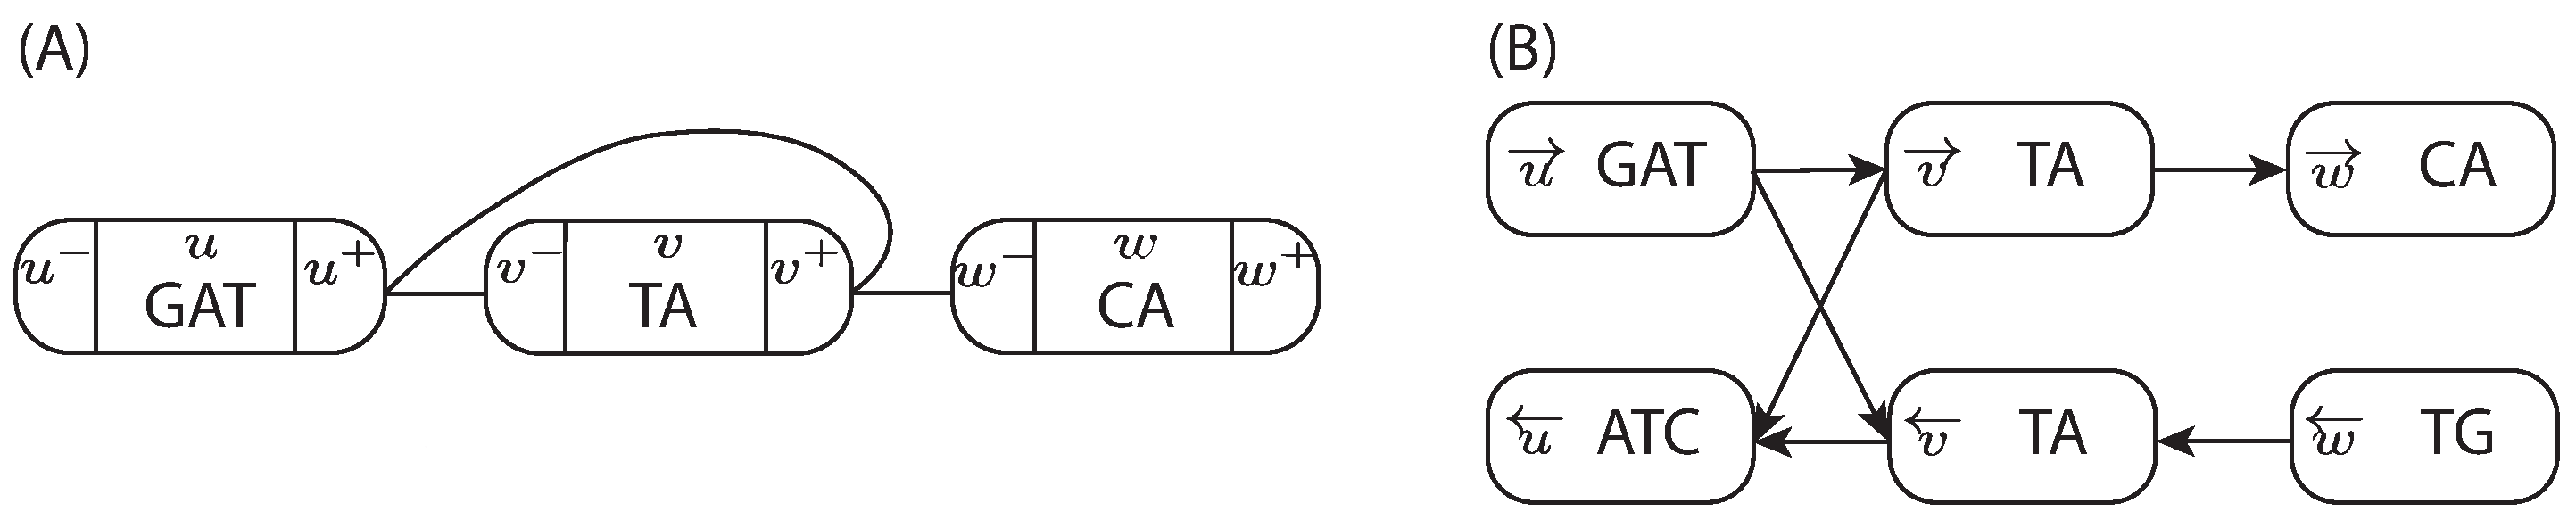
\includegraphics[width=\linewidth]{aim2_supplement_graph_example.pdf}
    \caption[Sequence graph example]{\textbf{Sequence graph example.}
      (A) A sequence graph with three nodes $u$, $v$, and $w$, with labels $\nodelabel{u} =$ GAT, $\nodelabel{v} =$ TA, and $\nodelabel{w} =$ CA. Node sides $\leftside{x}$ and $\rightside{x}$ are marked for each node $x$.
      (B) The same graph as a directed graph with each visit $\forwardnode{x}$ and $\reversenode{x}$ a separate node.
    }
    \label{fig:aim2_supplement_graph-example}
    \label{fig:first}
\end{figure}



\begin{figure}[H]
    \centering
    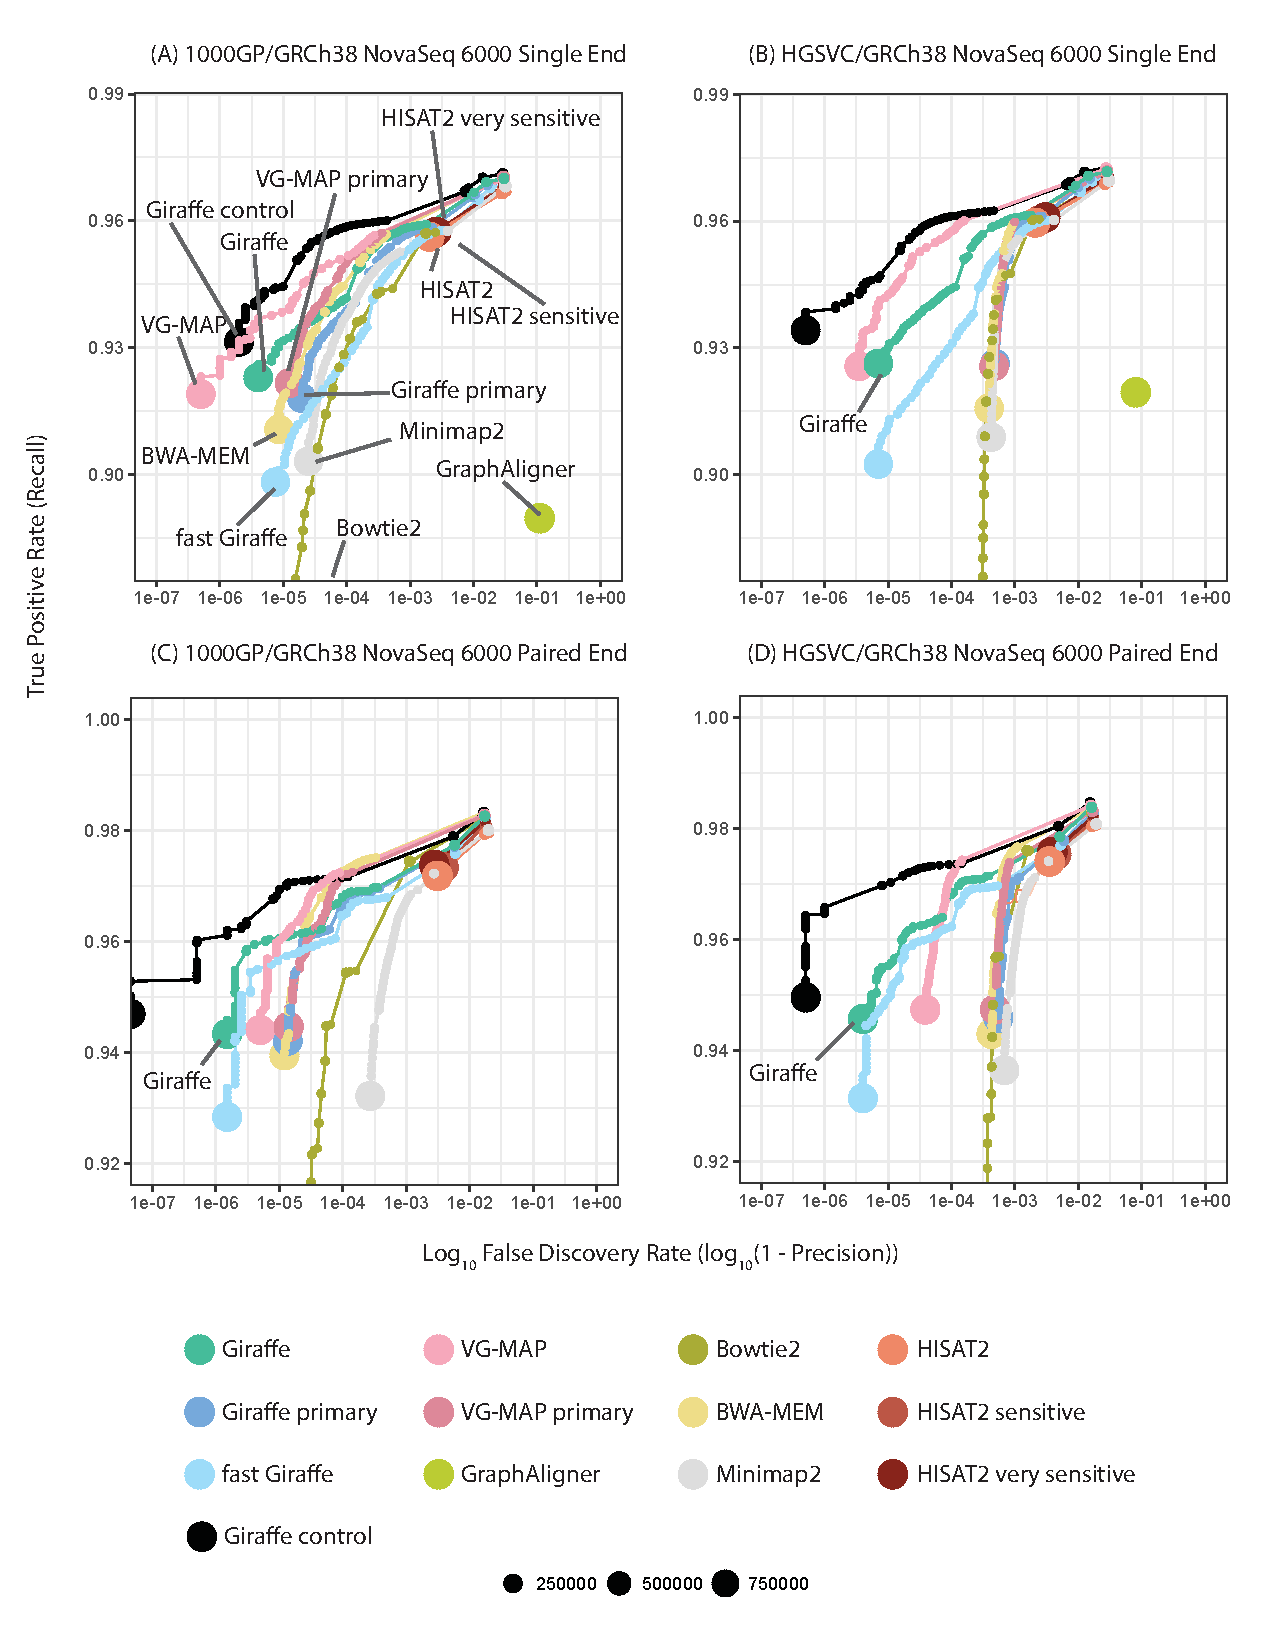
\includegraphics[width=.6\linewidth]{aim2_supplement_novaseq6000-all.pdf}
    \caption[Simulated read mapping with NovaSeq 6000 reads]{\textbf{Simulated read mapping with NovaSeq 6000 reads.} Each panel shows 1-precision (FDR) vs. recall for a simulated read mapping experiment. Reads were simulated to match 150bp Illumina NovaSeq 6000 reads and were mapped either as single ended reads (A,B) or as paired end reads (C,D). We compared graph mappers (Giraffe, VG-MAP, GraphAligner, HISAT2) and linear mappers (BWA-MEM, Bowtie2, Minimap2) mapping to either the 1000GP graph and GRCh38 reference (A,C) or the HGSVC graph and GRCh38 reference (B,D). For Giraffe, we mapped to a 64 haplotype sampled GBWT for the 1000GP graph and to the full GBWT for the HGSVC graph. In addition to aligning to the 1000GP and HGSVC graphs, we also used Giraffe and VG-MAP to align to primary graphs containing only the GRCh38 reference. We also ran Giraffe and HISAT2 using different pre-defined parameterizations in addition to the default settings: fast Giraffe and HISAT2 sensitive and very sensitive. For a positive control, we aligned reads to our positive control graphs using Giraffe run with a more exhaustive parameterization.
    Reads were stratified by their mapping quality. Each point in the plot represents to a mapping quality value and the size of a point corresponds the number of reads it represents. GraphAligner did not assign mapping qualities, so it is represented as a single point. For the remaining mappers, the mapping quality values varied from 0 to 60, except for Bowtie2, which had a maximum mapping quality of 42.}
    \label{fig:aim2_supplement_novaseq_rocs}
\end{figure}

\begin{figure}[H]
    \centering
    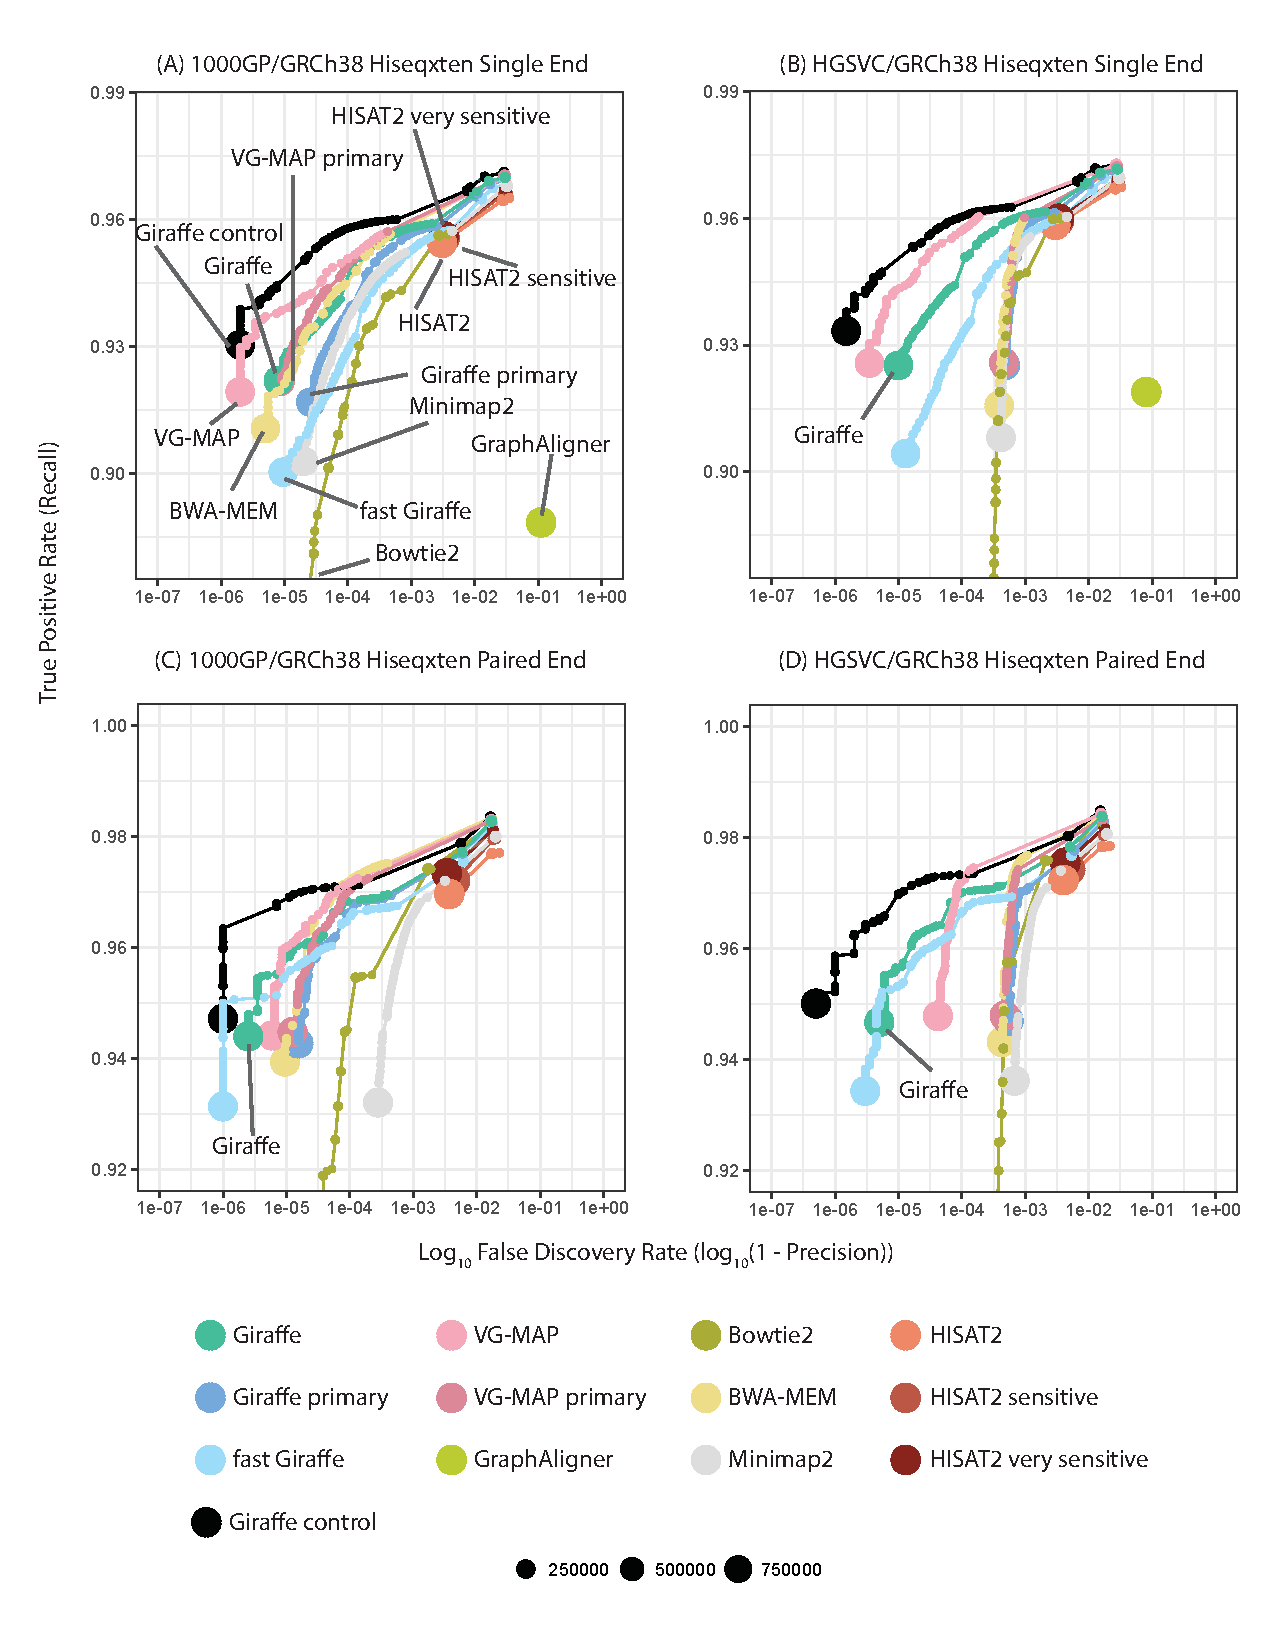
\includegraphics[width=.8\linewidth]{aim2_supplement_hiseqxten-all.pdf}
    \caption[Simulated read mapping with HiSeq X Ten reads]{\textbf{Simulated read mapping with HiSeq X Ten reads.} Each panel shows 1-precision (FDR) vs. recall for a simulated read mapping experiment. Reads were mapped as single-end (A, B) or paired-end (C, D) to the 1000GP graph and GRCh38 reference (A, C) or the HGSVC graph and GRCh38 reference (B, D).}
    \label{fig:aim2_supplement_hiseqxten_rocs}
\end{figure}
\begin{figure}[H]
    \centering
    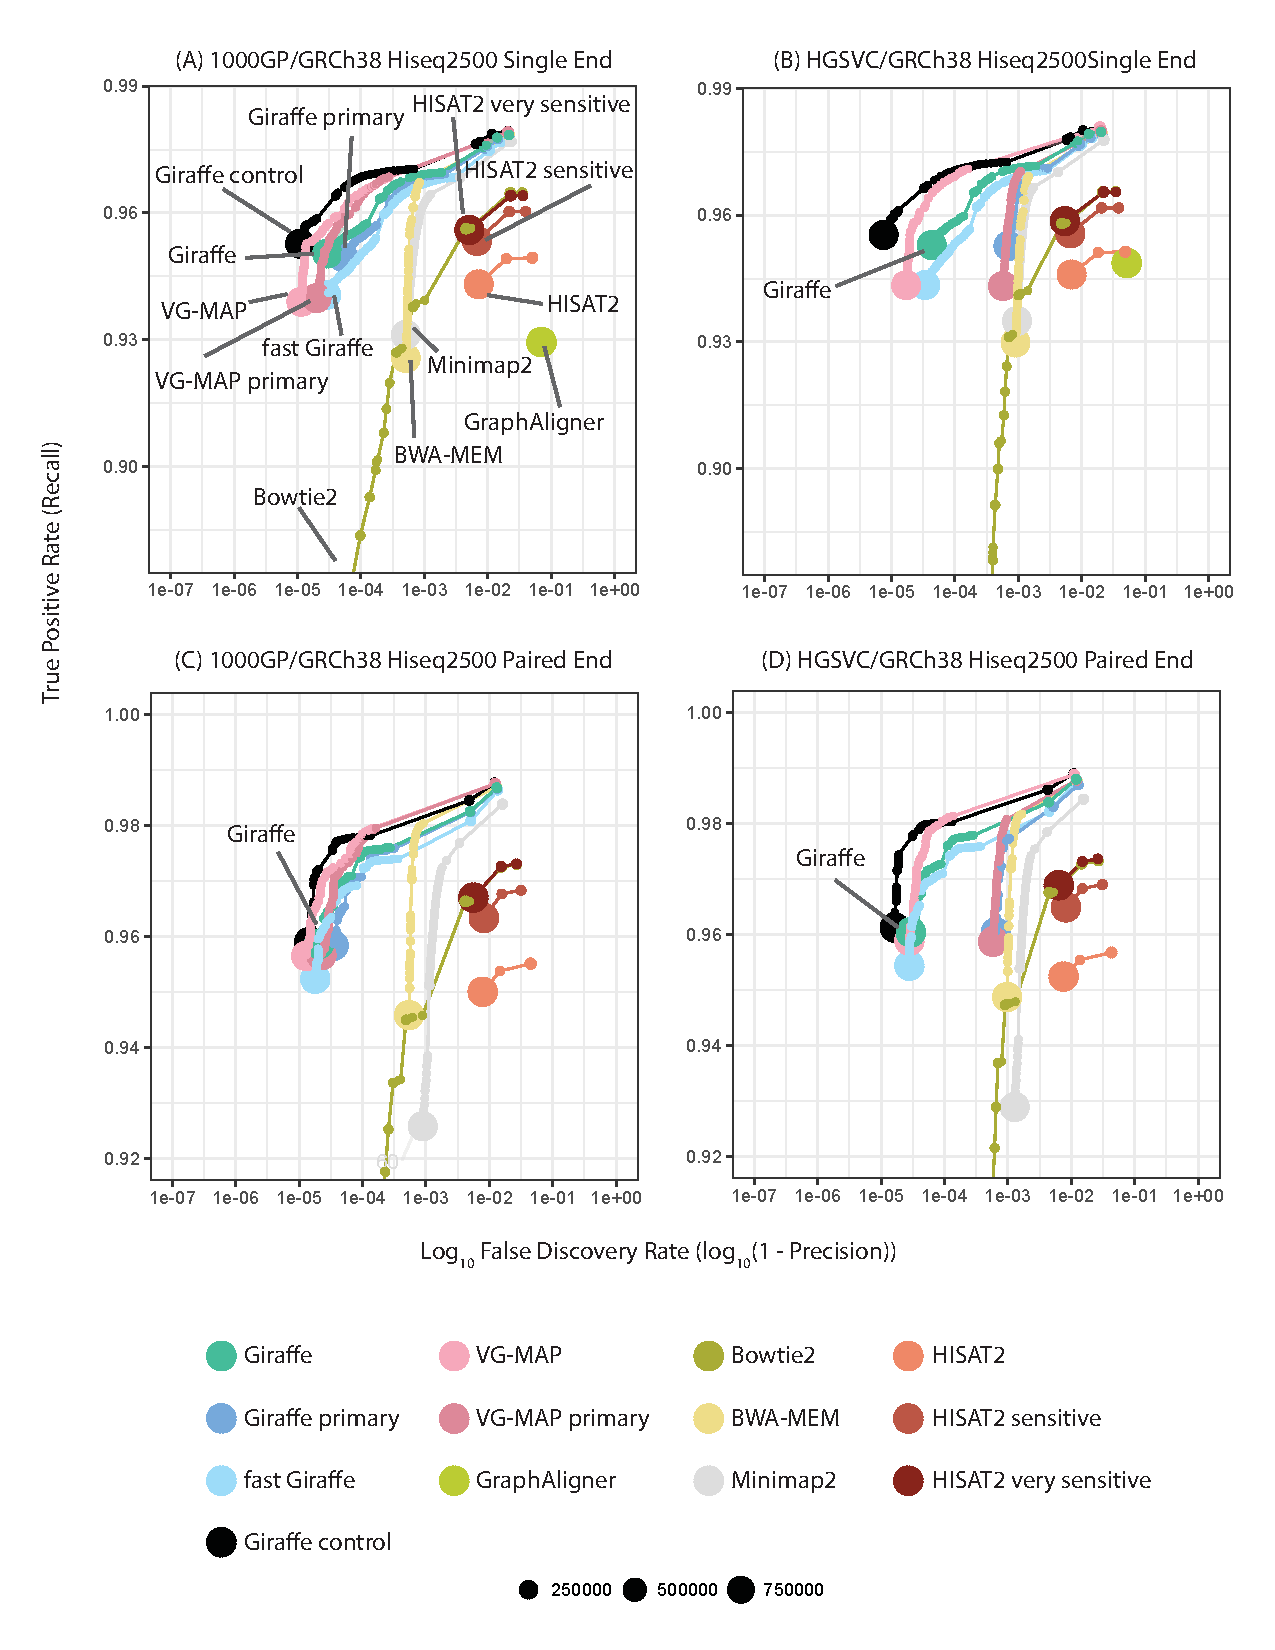
\includegraphics[width=.8\linewidth]{aim2_supplement_hiseq2500-all.pdf}
    \caption[Simulated read mapping with HiSeq 2500 reads]{\textbf{Simulated read mapping with HiSeq 2500 reads.} Each panel shows 1-precision (FDR) vs. recall for a simulated read mapping experiment. Reads were mapped as single-end (A, B) or paired-end (C, D) to the 1000GP graph and GRCh38 reference (A, C) or the HGSVC graph and GRCh38 reference (B, D).}
    \label{fig:aim2_supplement_hiseq2500_rocs}
\end{figure}
\begin{figure}[H]
    \centering
    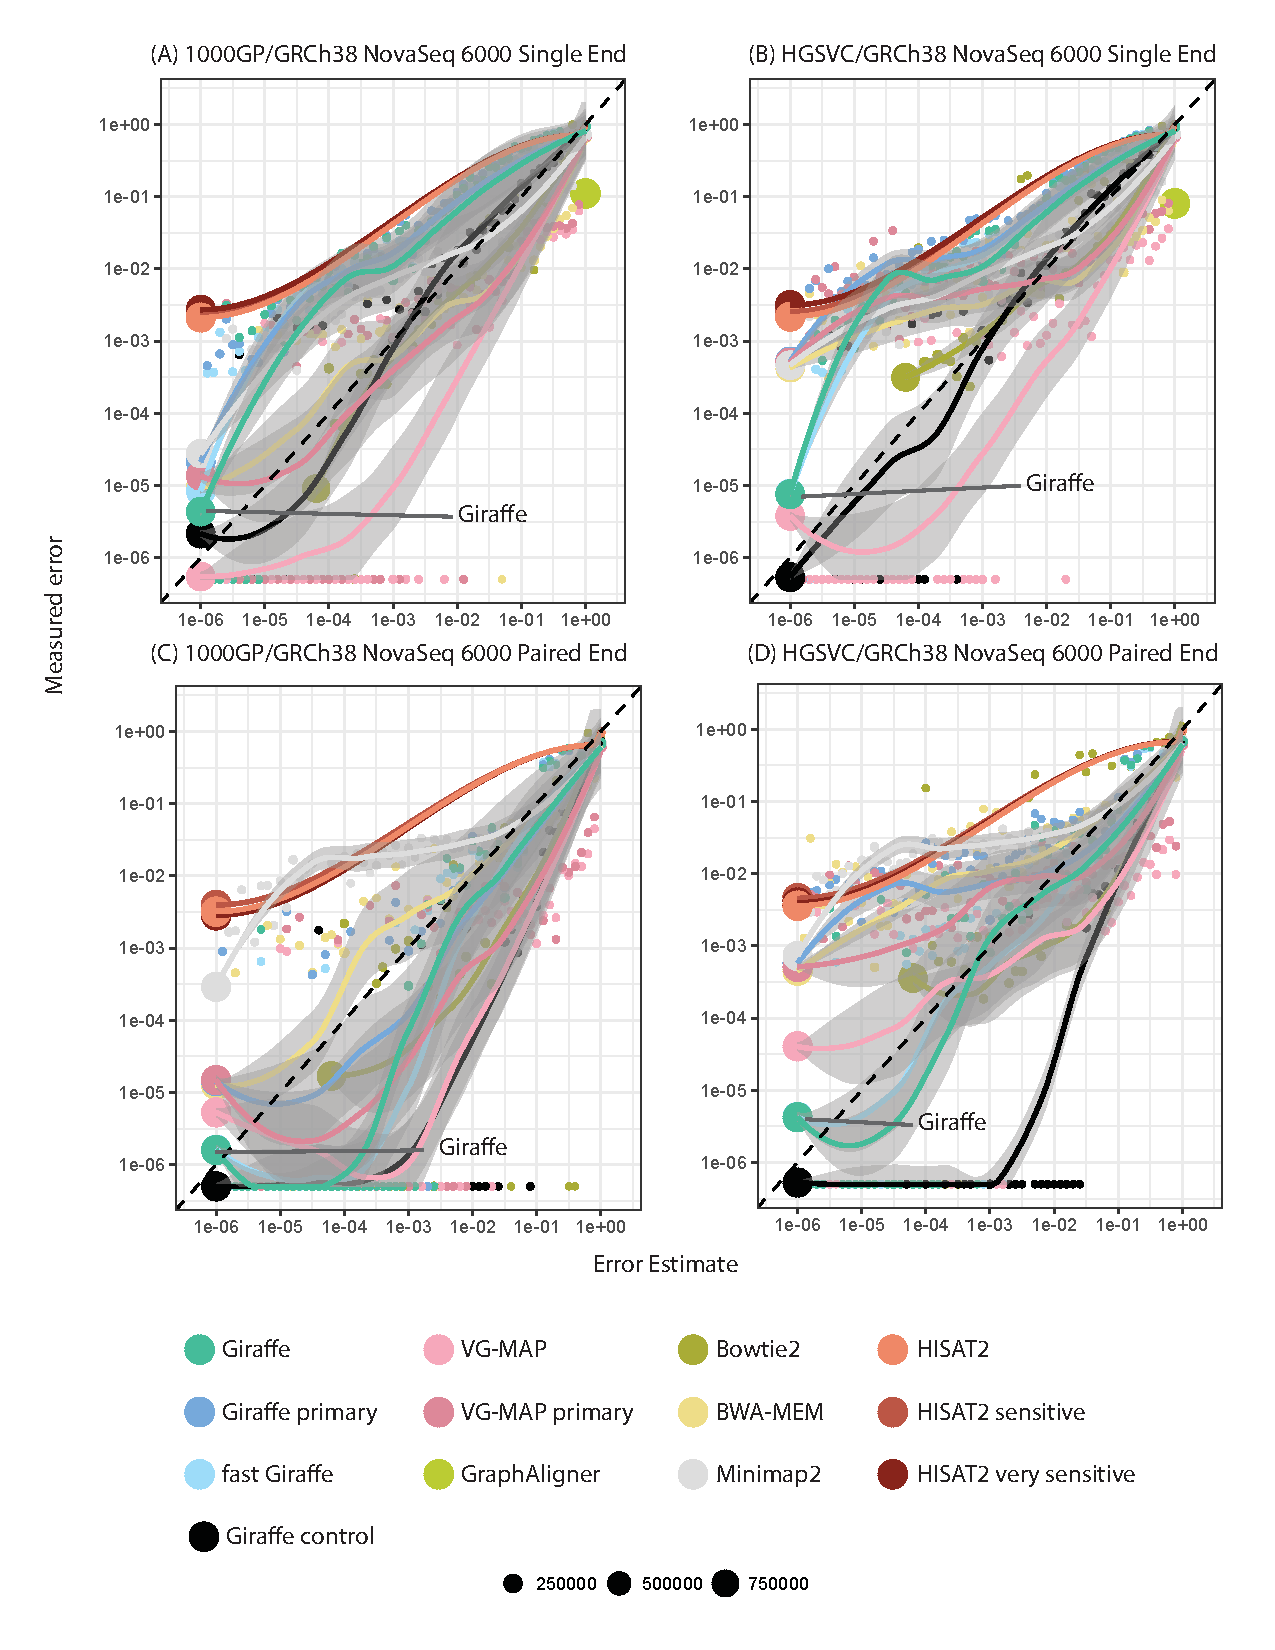
\includegraphics[width=.8\linewidth]{aim2_supplement_novaseq6000-qq.pdf}
    \caption[QQ plot for simulated read mapping with NovaSeq 6000 reads]{\textbf{QQ plot for simulated read mapping with NovaSeq 6000 reads.} Each panel shows a QQ plot for a simulated read mapping experiment. Reads were mapped as single-end (A, B) or paired-end (C, D) to the 1000GP graph and GRCh38 reference (A, C) or the HGSVC graph and GRCh38 reference (B, D).}
    \label{fig:aim2_supplement_novaseq6000_qq}
\end{figure}
\begin{figure}[H]
    \centering
    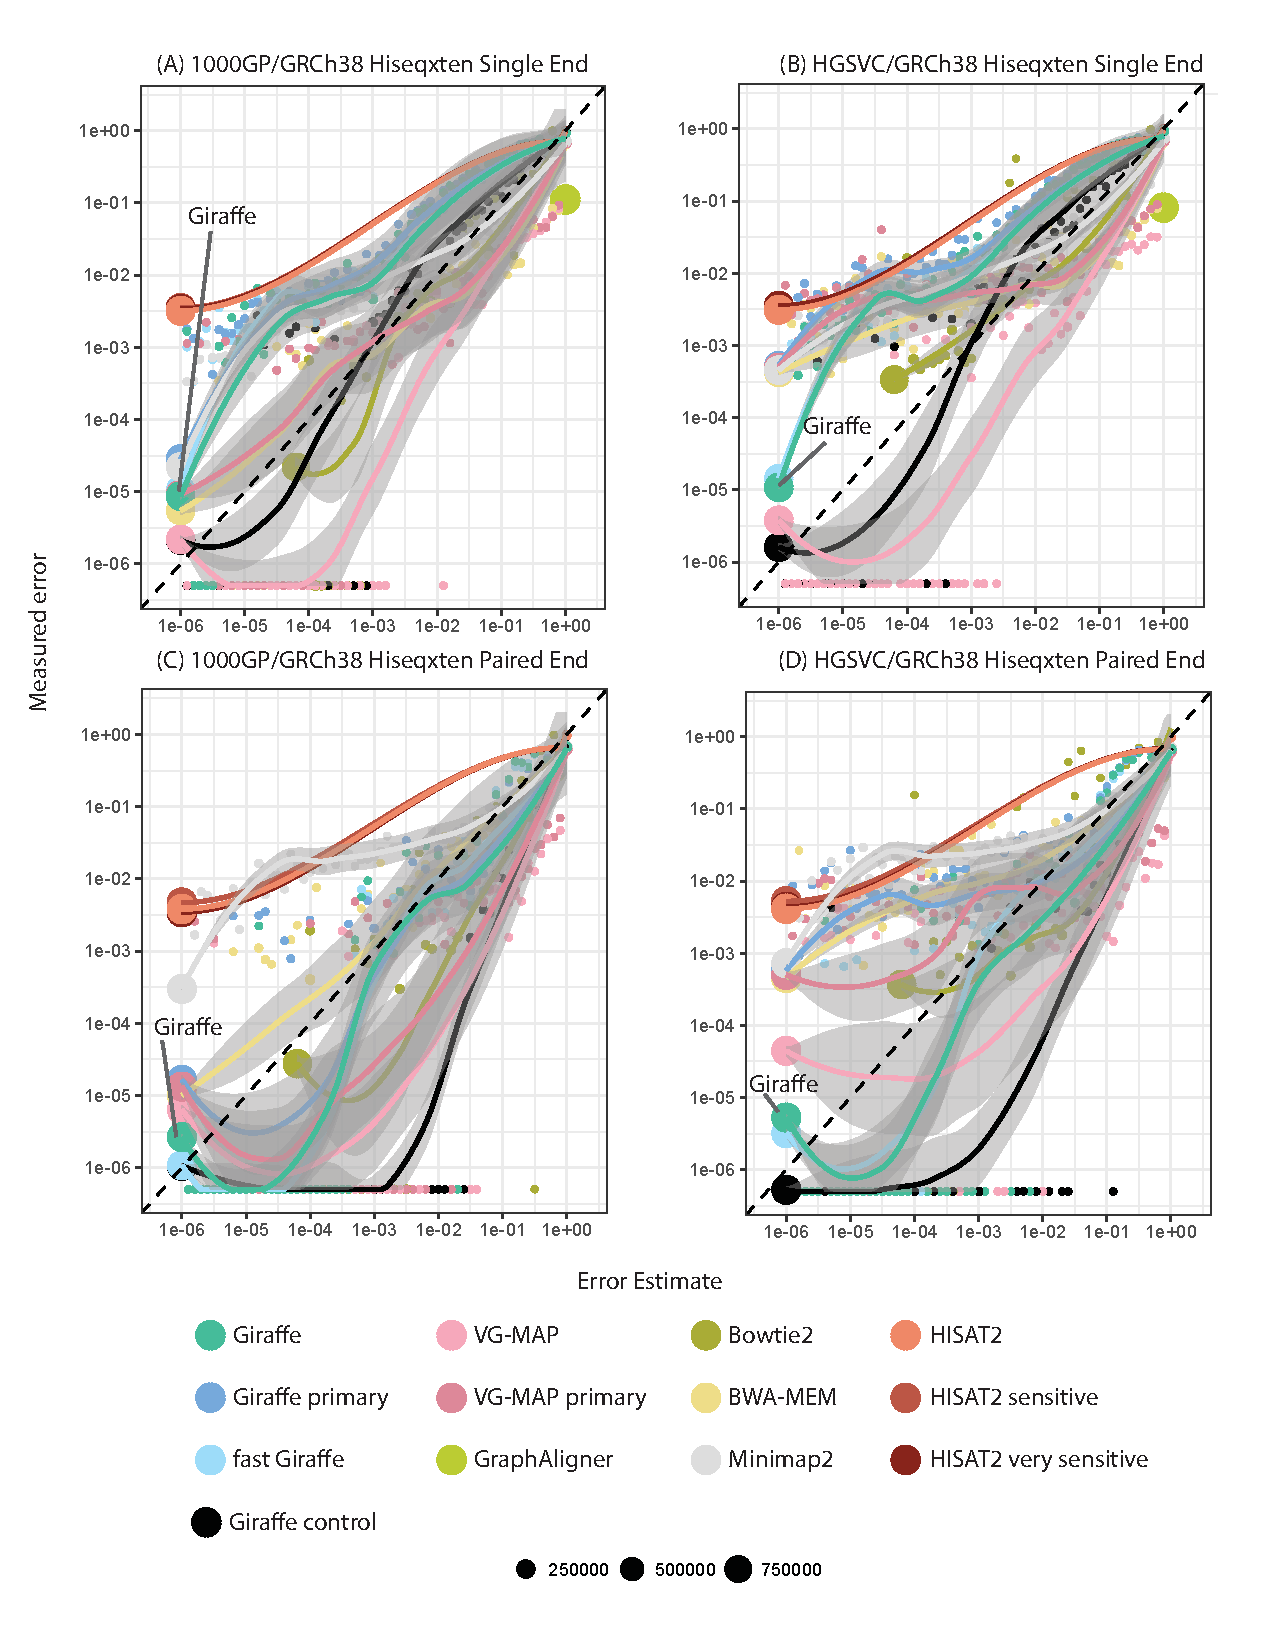
\includegraphics[width=.8\linewidth]{aim2_supplement_hiseqxten-qq.pdf}
    \caption[QQ plot for simulated read mapping with HiSeq X Ten reads]{\textbf{QQ plot for simulated read mapping with HiSeq X Ten reads.} Each panel shows a QQ plot for a simulated read mapping experiment. Reads were mapped as single-end (A, B) or paired-end (C, D) to the 1000GP graph and GRCh38 reference (A, C) or the HGSVC graph and GRCh38 reference (B, D).}
    \label{fig:aim2_supplement_hiseqxten_qq}
\end{figure}
\begin{figure}[H]
    \centering
    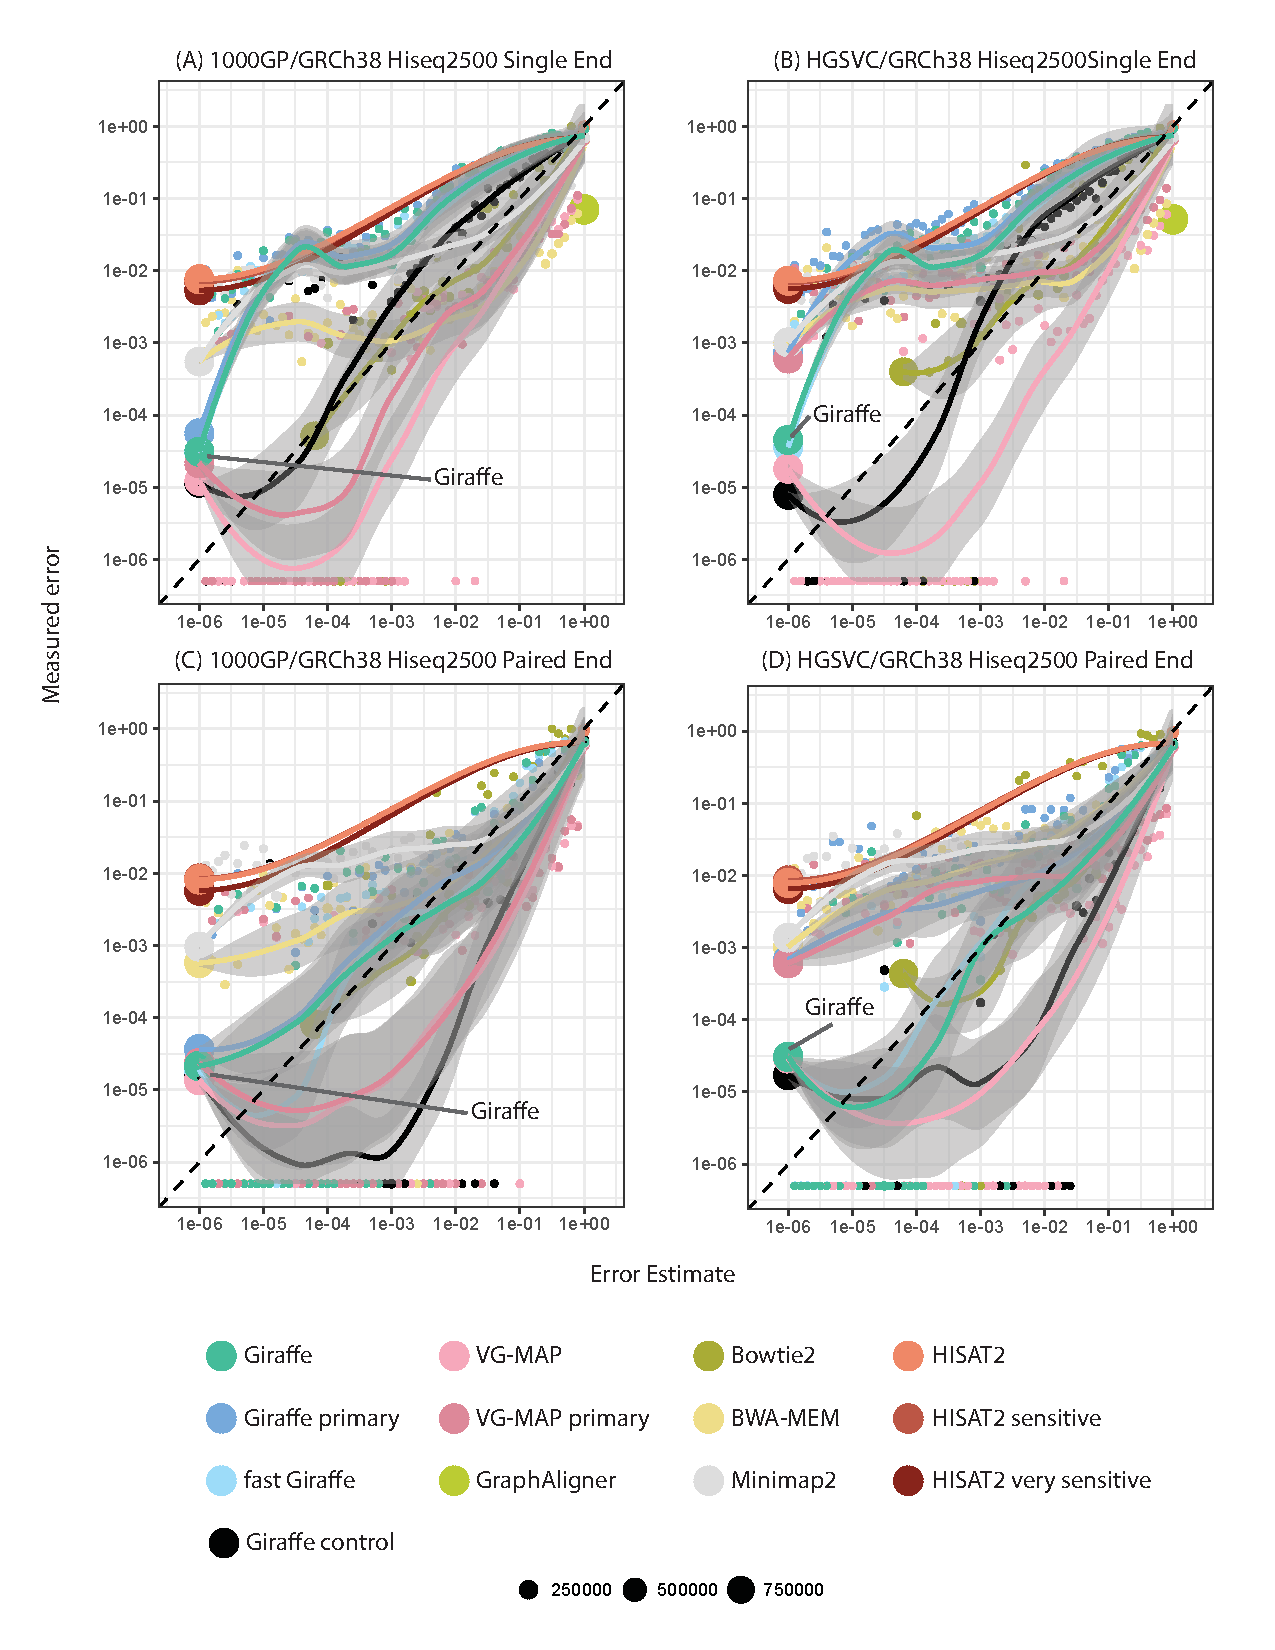
\includegraphics[width=.8\linewidth]{aim2_supplement_hiseq2500-qq.pdf}
    \caption[QQ plot for simulated read mapping with HiSeq 2500 reads]{\textbf{QQ plot for simulated read mapping with HiSeq 2500 reads.} Each panel shows a QQ plot for a simulated read mapping experiment. Reads were mapped as single-end (A, B) or paired-end (C, D) to the 1000GP graph and GRCh38 reference (A, C) or the HGSVC graph and GRCh38 reference (B, D).}
    \label{fig:aim2_supplement_hiseq2500_qq}
\end{figure}

\begin{figure}[H]
    \centering
    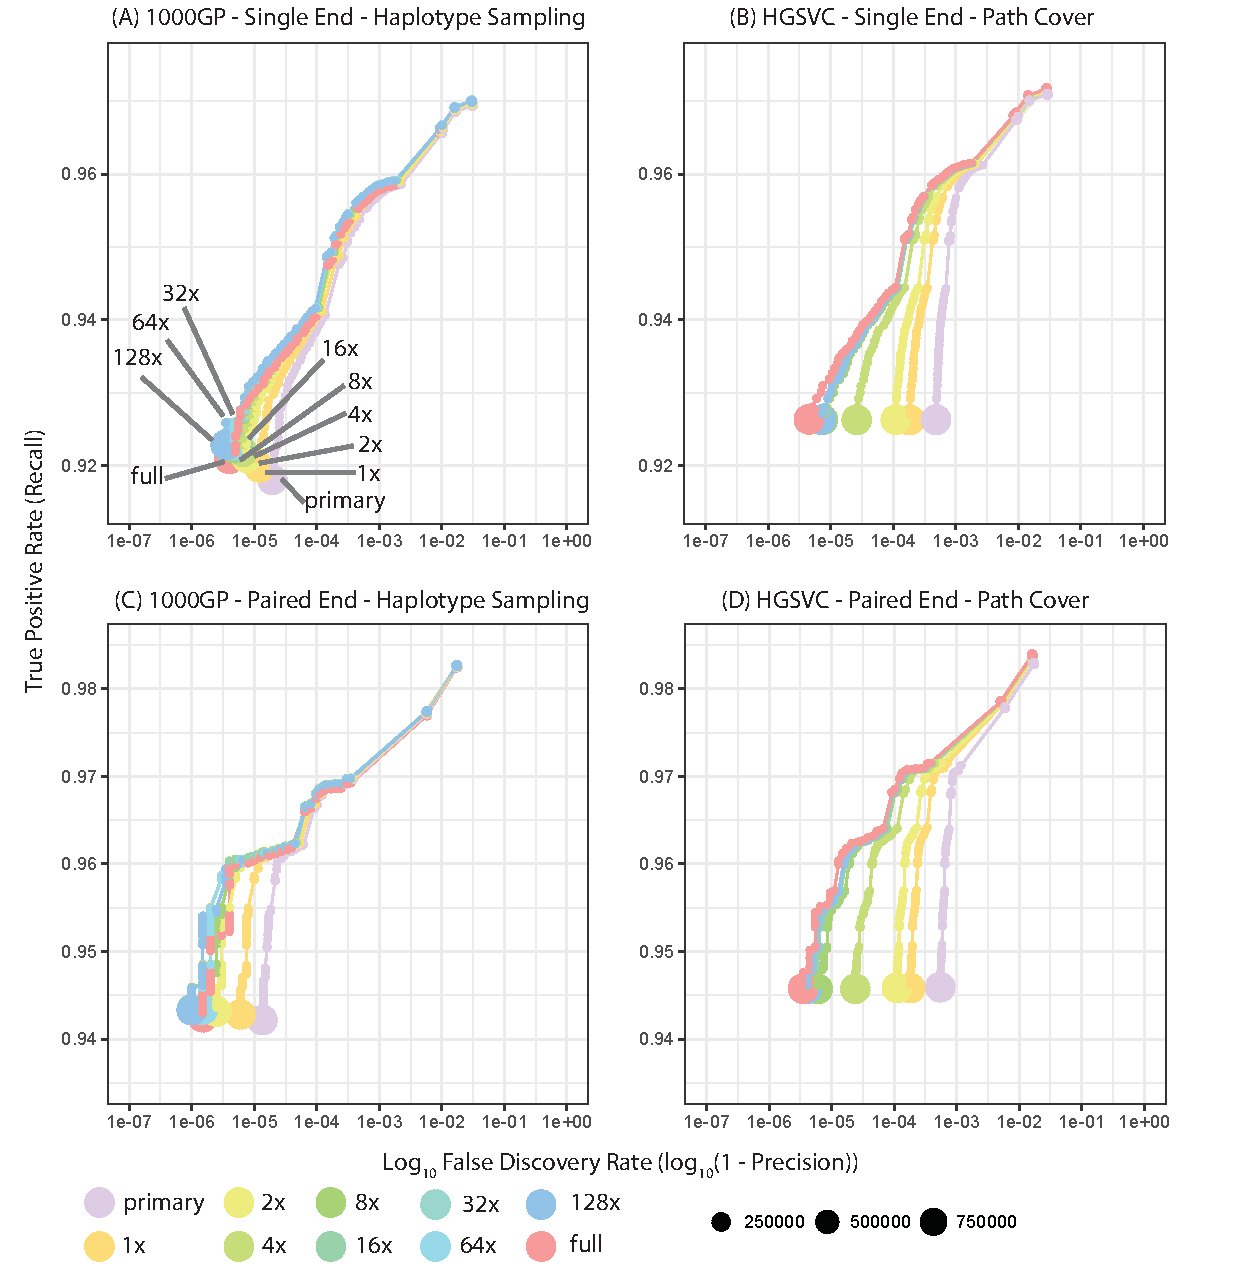
\includegraphics[width=.9\linewidth]{aim2_haplotype_sampling.pdf}
    \caption[Assessing haplotype sampling and path cover]{\textbf{Assessing haplotype sampling and path cover.} Each panel shows recall vs. FDR for a simulated read mapping experiment. (A,C) Haplotype sampling, for samplings from 1 to 128 using the 1000GP derived graph (Table \ref{tab:mapping_accuracy_1000gp_sampled_gbwt}). Includes for comparison a graph containing just the primary reference (here GRCh38) and, separately, the full 1000GP GBWT. For both (A) single-ended and (C) paired-end mapping, performance saturates at around 64x coverage of sampled haplotypes, and exceeds that of mapping to the full GBWT containing all haplotypes. (B,D) Analogous path cover experiments, using the HGSVC graph (Table \ref{tab:mapping_accuracy_hgsvc_cover_gbwt}). All GBWT indexes were evaluated with simulated NovaSeq 6000 reads.}
    \label{fig:aim2_supplement_haplotype_sampling}
\end{figure}

\begin{figure}[H]
    \centering
    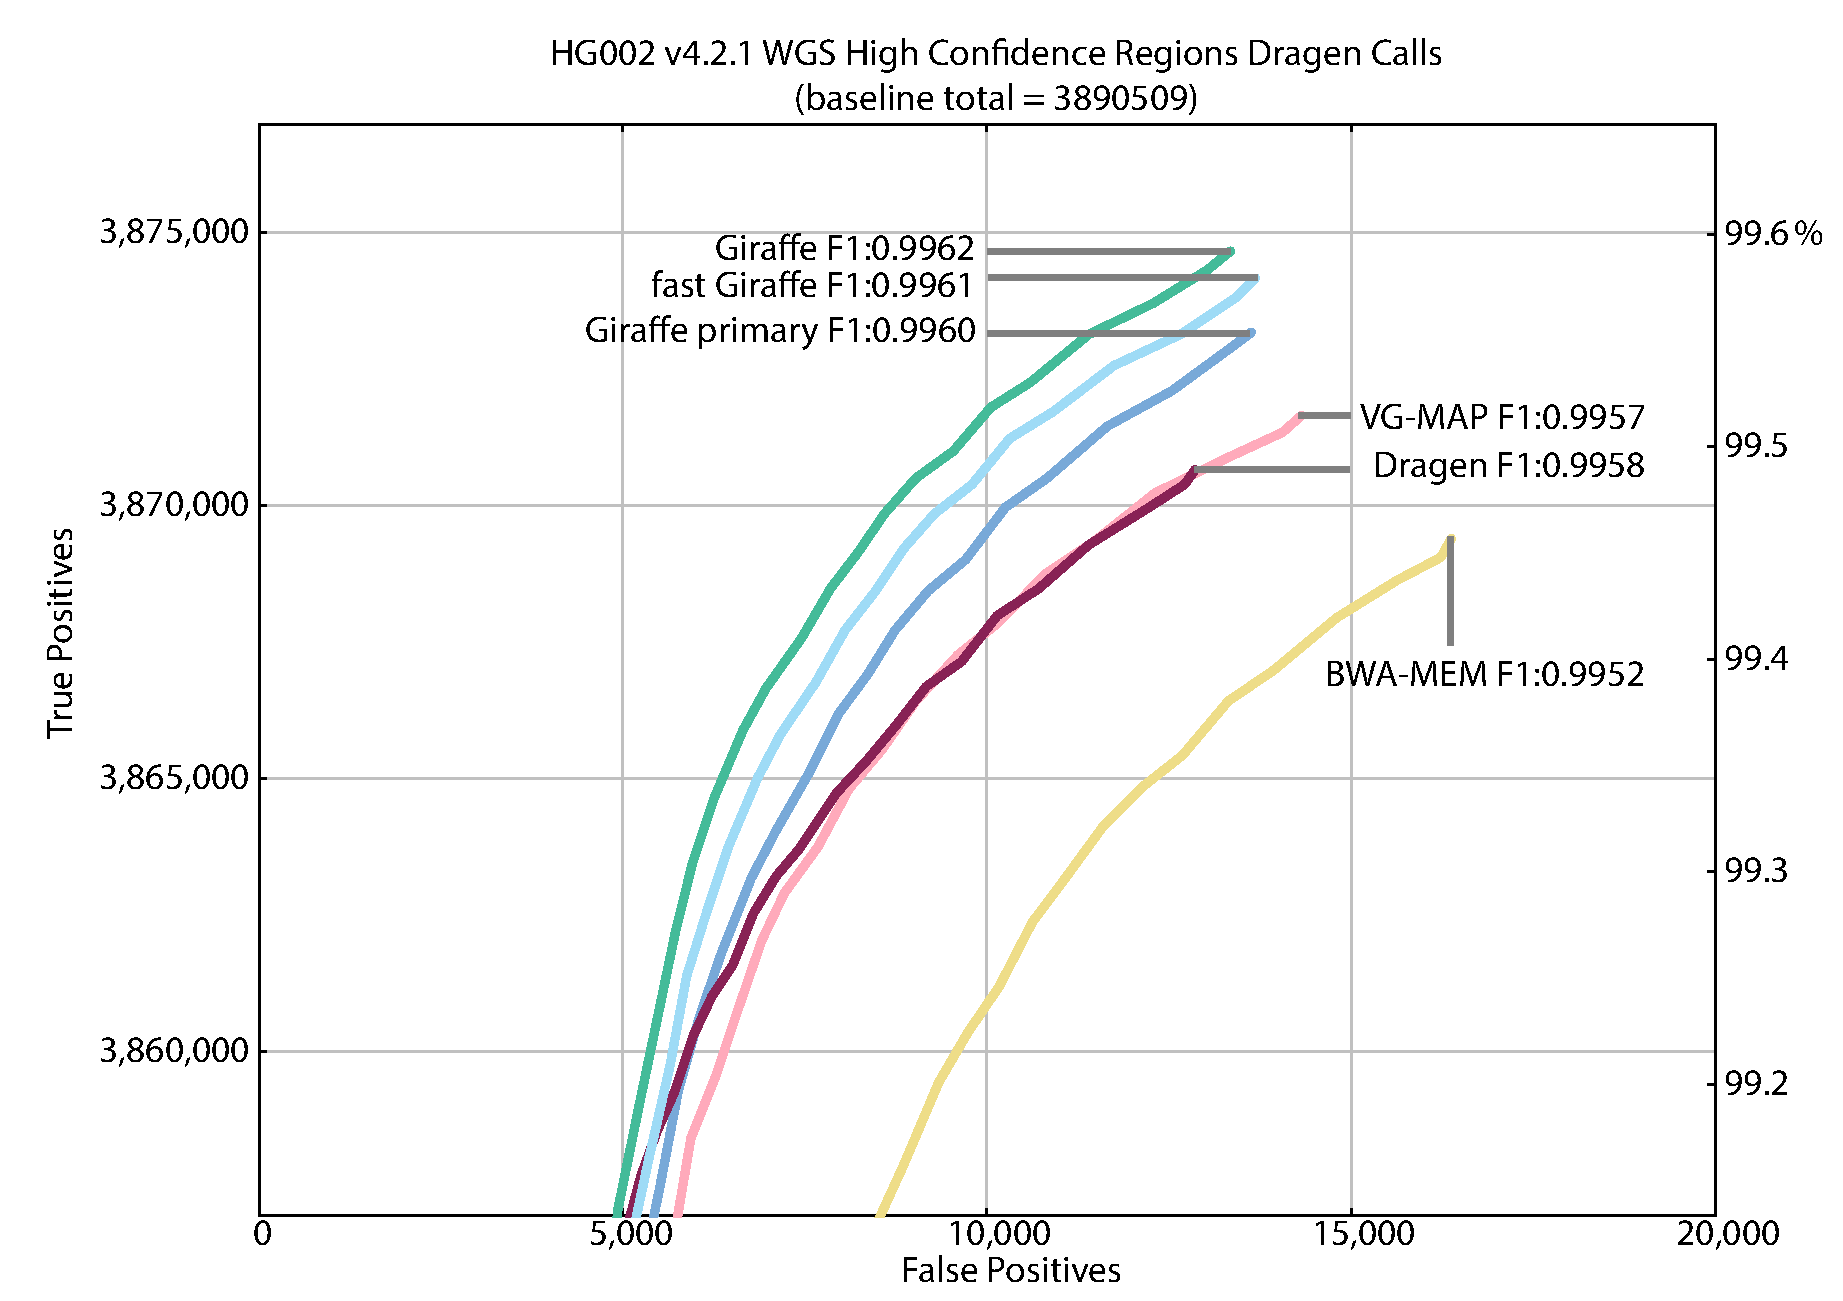
\includegraphics[width=\linewidth]{HG002_v4.2.1_high_conf.35x_250bp.wgs.vcfevalroc.pdf}
    \caption[Genotyping evaluation for the Dragen genotyper with projected mappings from Giraffe and other mappers]{True positive and false positive genotypes made using the Dragen genotyper with projected mappings from Giraffe and other mappers, using 250bp paired-end reads from the HG002 GIAB sample and evaluated against the HG002 GIAB v4.2.1 truth variant call sets in high confidence regions. The ROC curve discrimination threshold is based on variant call quality.}
    \label{fig:250bp_genotyping}
\end{figure}
\begin{figure}[H]
    \centering
    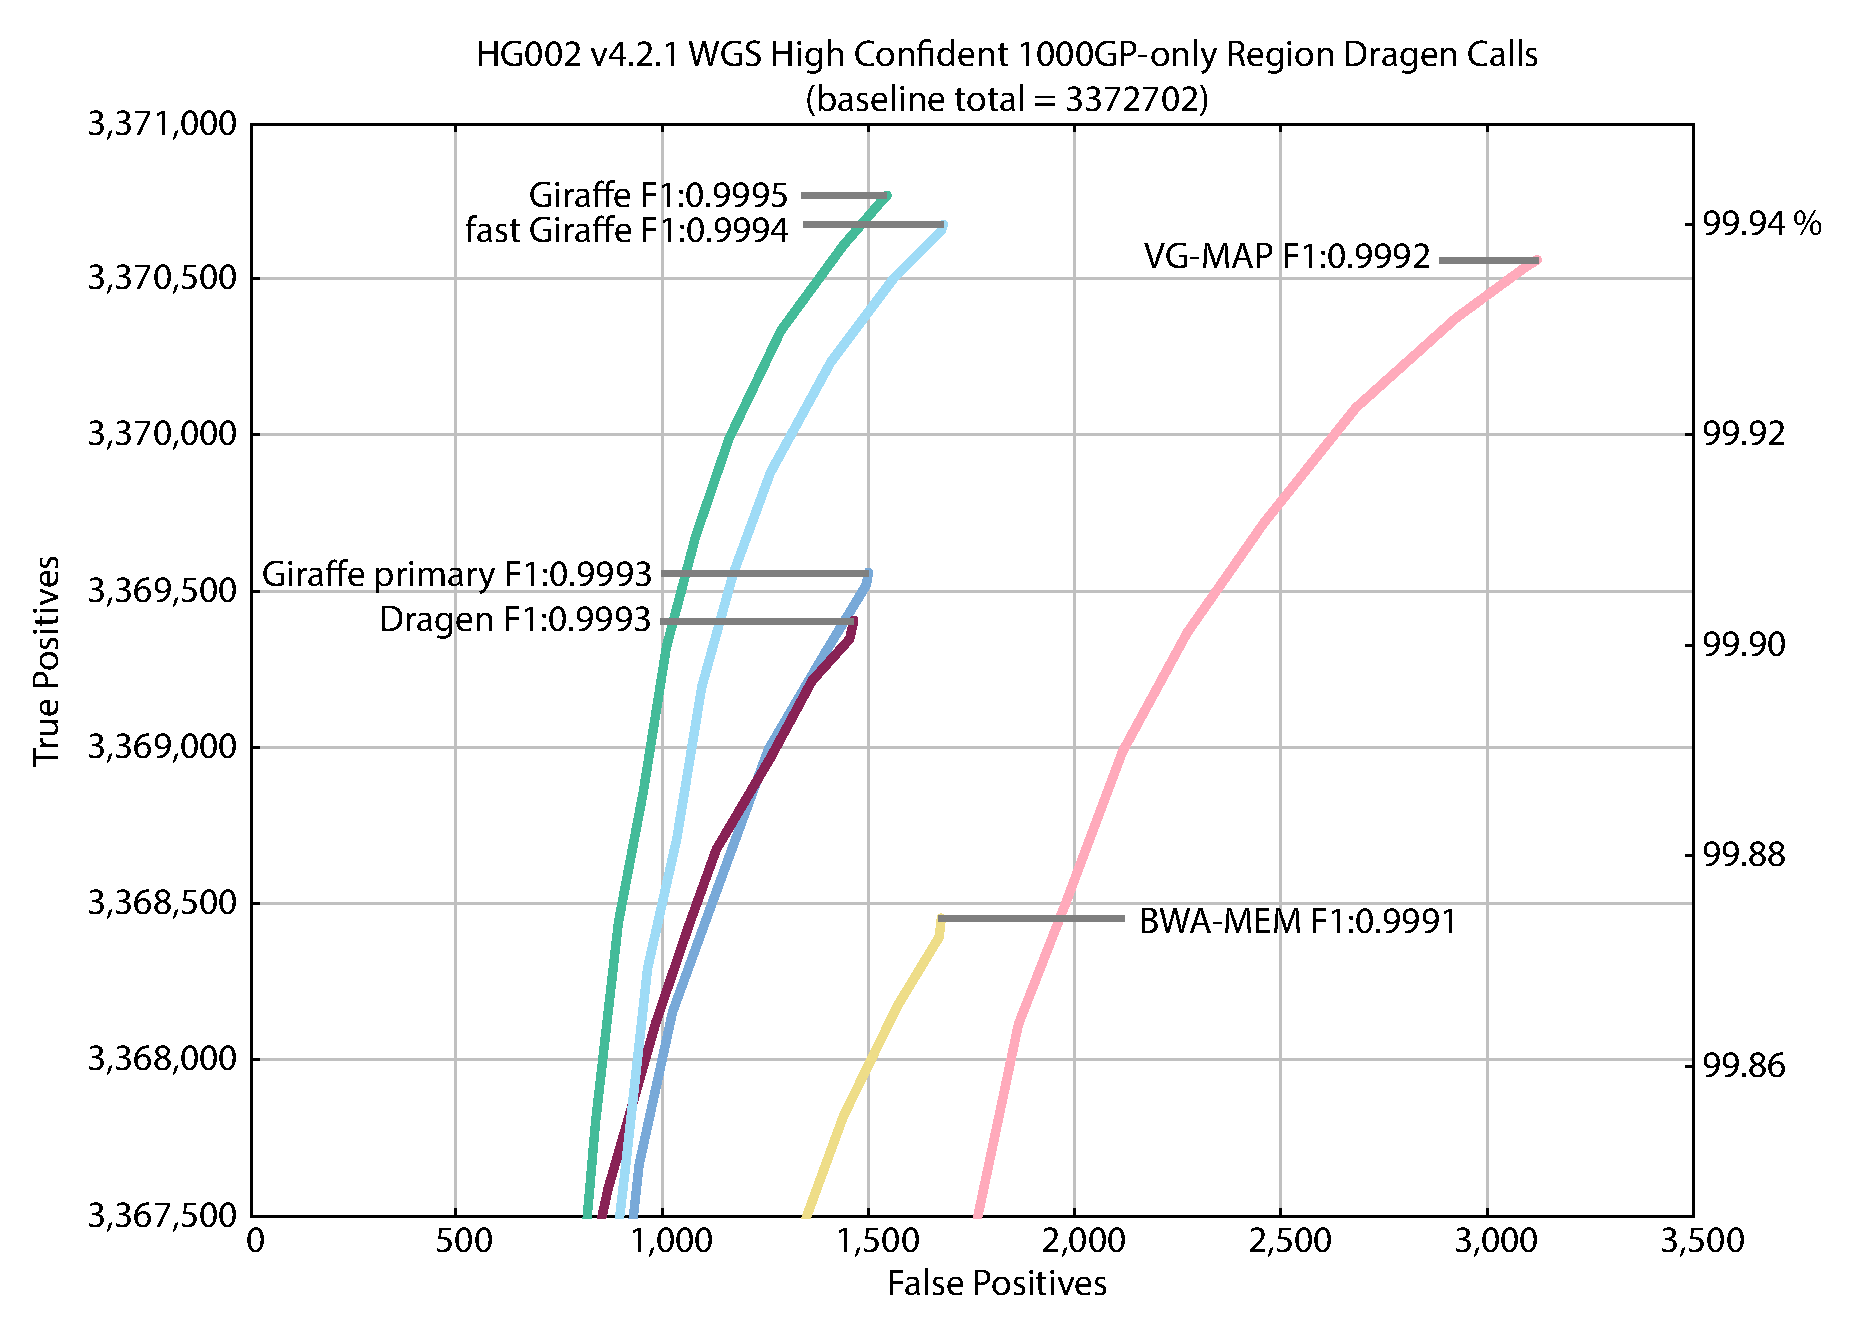
\includegraphics[width=\linewidth]{HG002_v4.2.1_high_conf.35x_150bp.wgs.vcfevalroc.1000GP_only.pdf}
    \caption[Genotyping evaluation for the Dragen genotyper with projected mappings from Giraffe and other mappers in 1000GP regions only]{True positive and false positive genotypes made using the Dragen genotyper with projected mappings from Giraffe and other mappers, using 150bp paired-end reads from the HG002 GIAB sample and evaluated against the HG002 GIAB v4.2.1 truth variant call sets in high confidence regions only within 1000GP variant regions. The ROC curve discrimination threshold is based on variant call quality.}
    \label{fig:150bp_genotyping_1000GP_only}
\end{figure}


\begin{figure}[H]
    \centering
    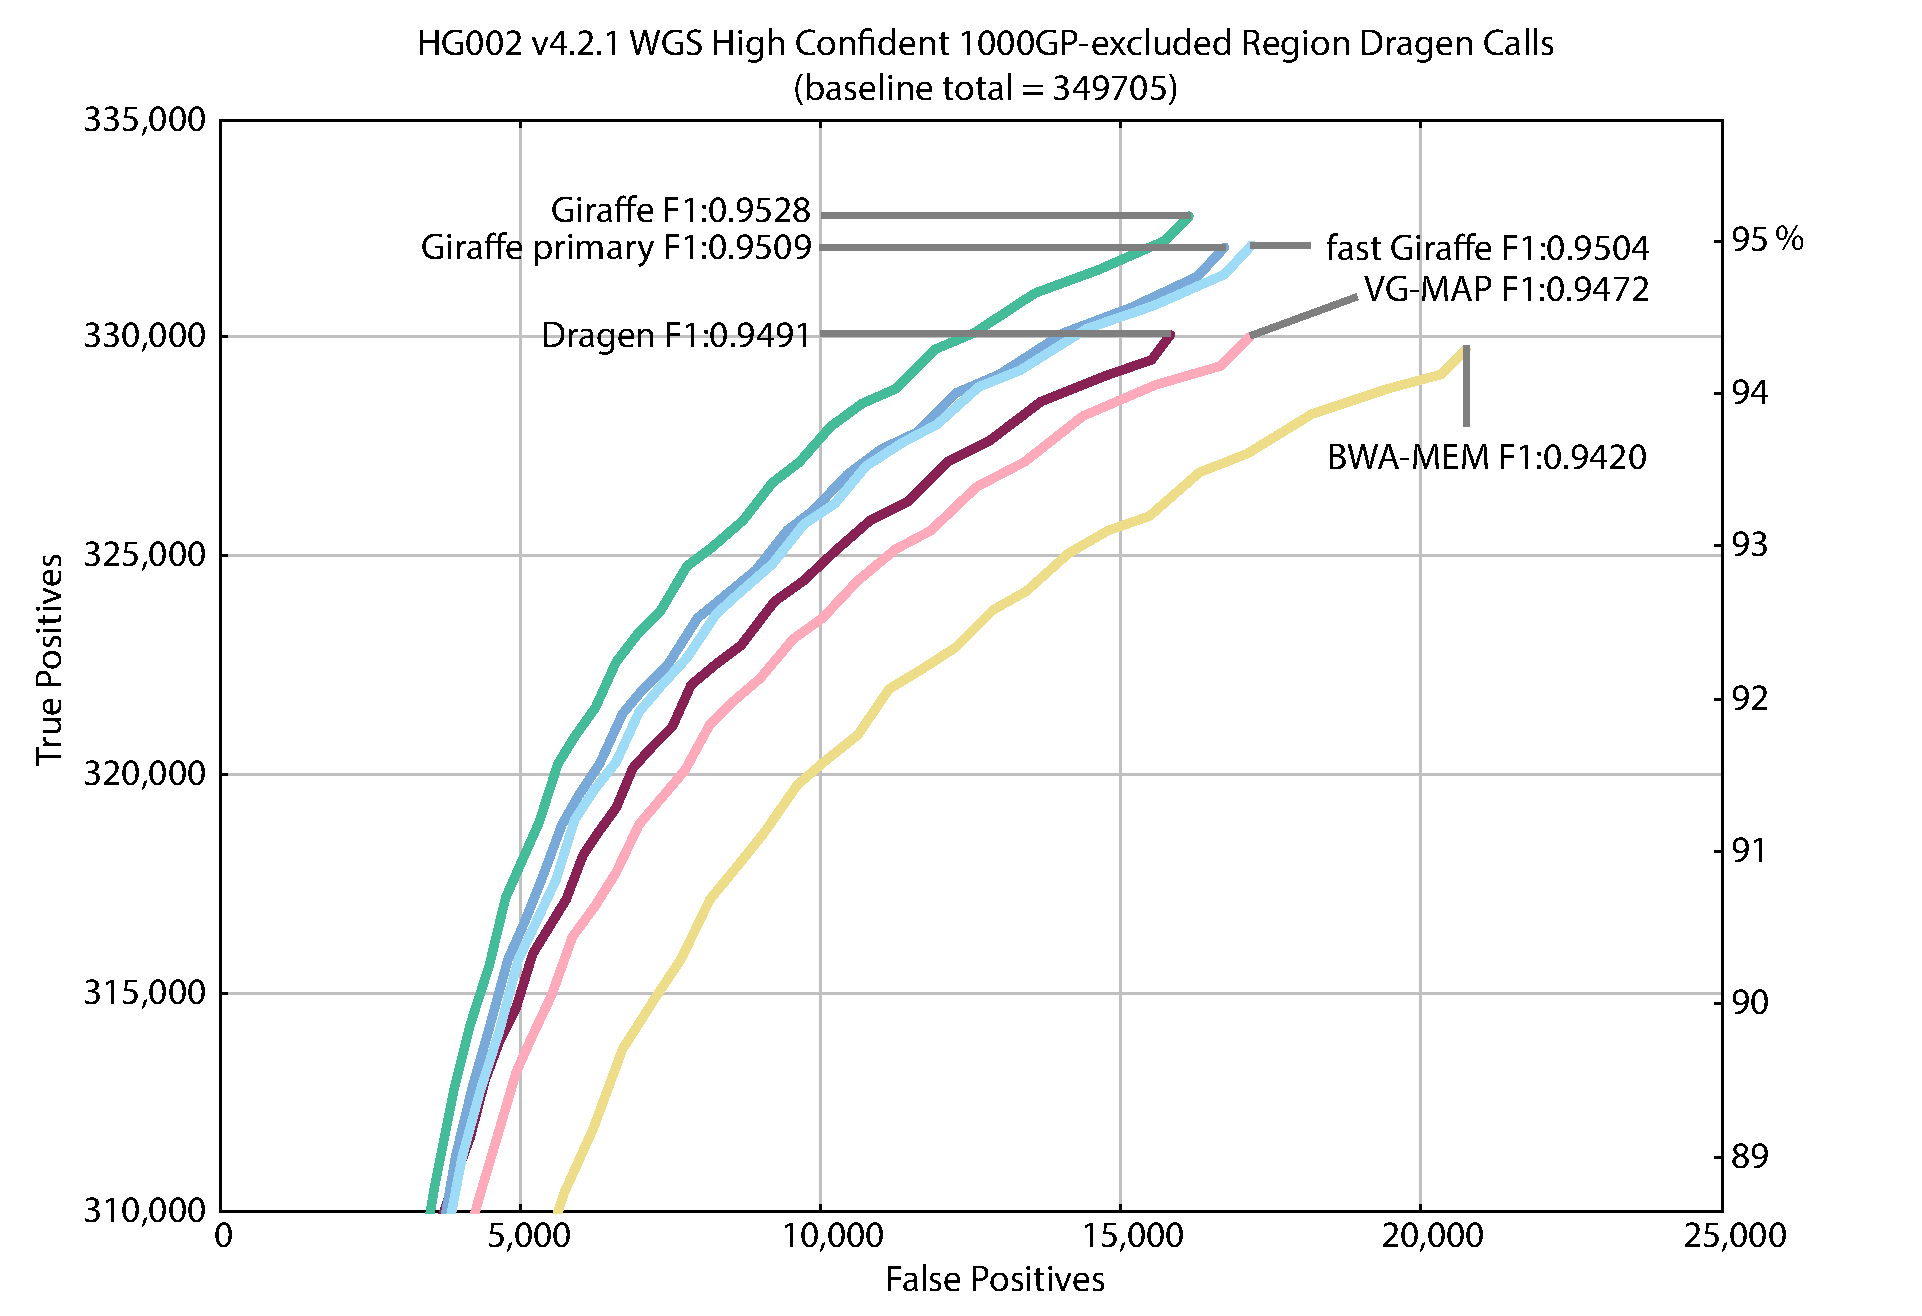
\includegraphics[width=\linewidth]{HG002_v4.2.1_high_conf.35x_150bp.wgs.vcfevalroc.1000GP_excluded.pdf}
    \caption[Genotyping evaluation for the Dragen genotyper with projected mappings from Giraffe and other mappers in 1000GP excluded regions]{True positive and false positive genotypes made using the Dragen genotyper with projected mappings from Giraffe and other mappers, using 150bp paired-end reads from the HG002 GIAB sample and evaluated against the HG002 GIAB v4.2.1 truth variant call sets in high confidence regions with 1000GP variant regions excluded. The ROC curve discrimination threshold is based on variant call quality.}
    \label{fig:150bp_genotyping_1000GP_excluded}
\end{figure}

\begin{figure}[H]
    \centering
    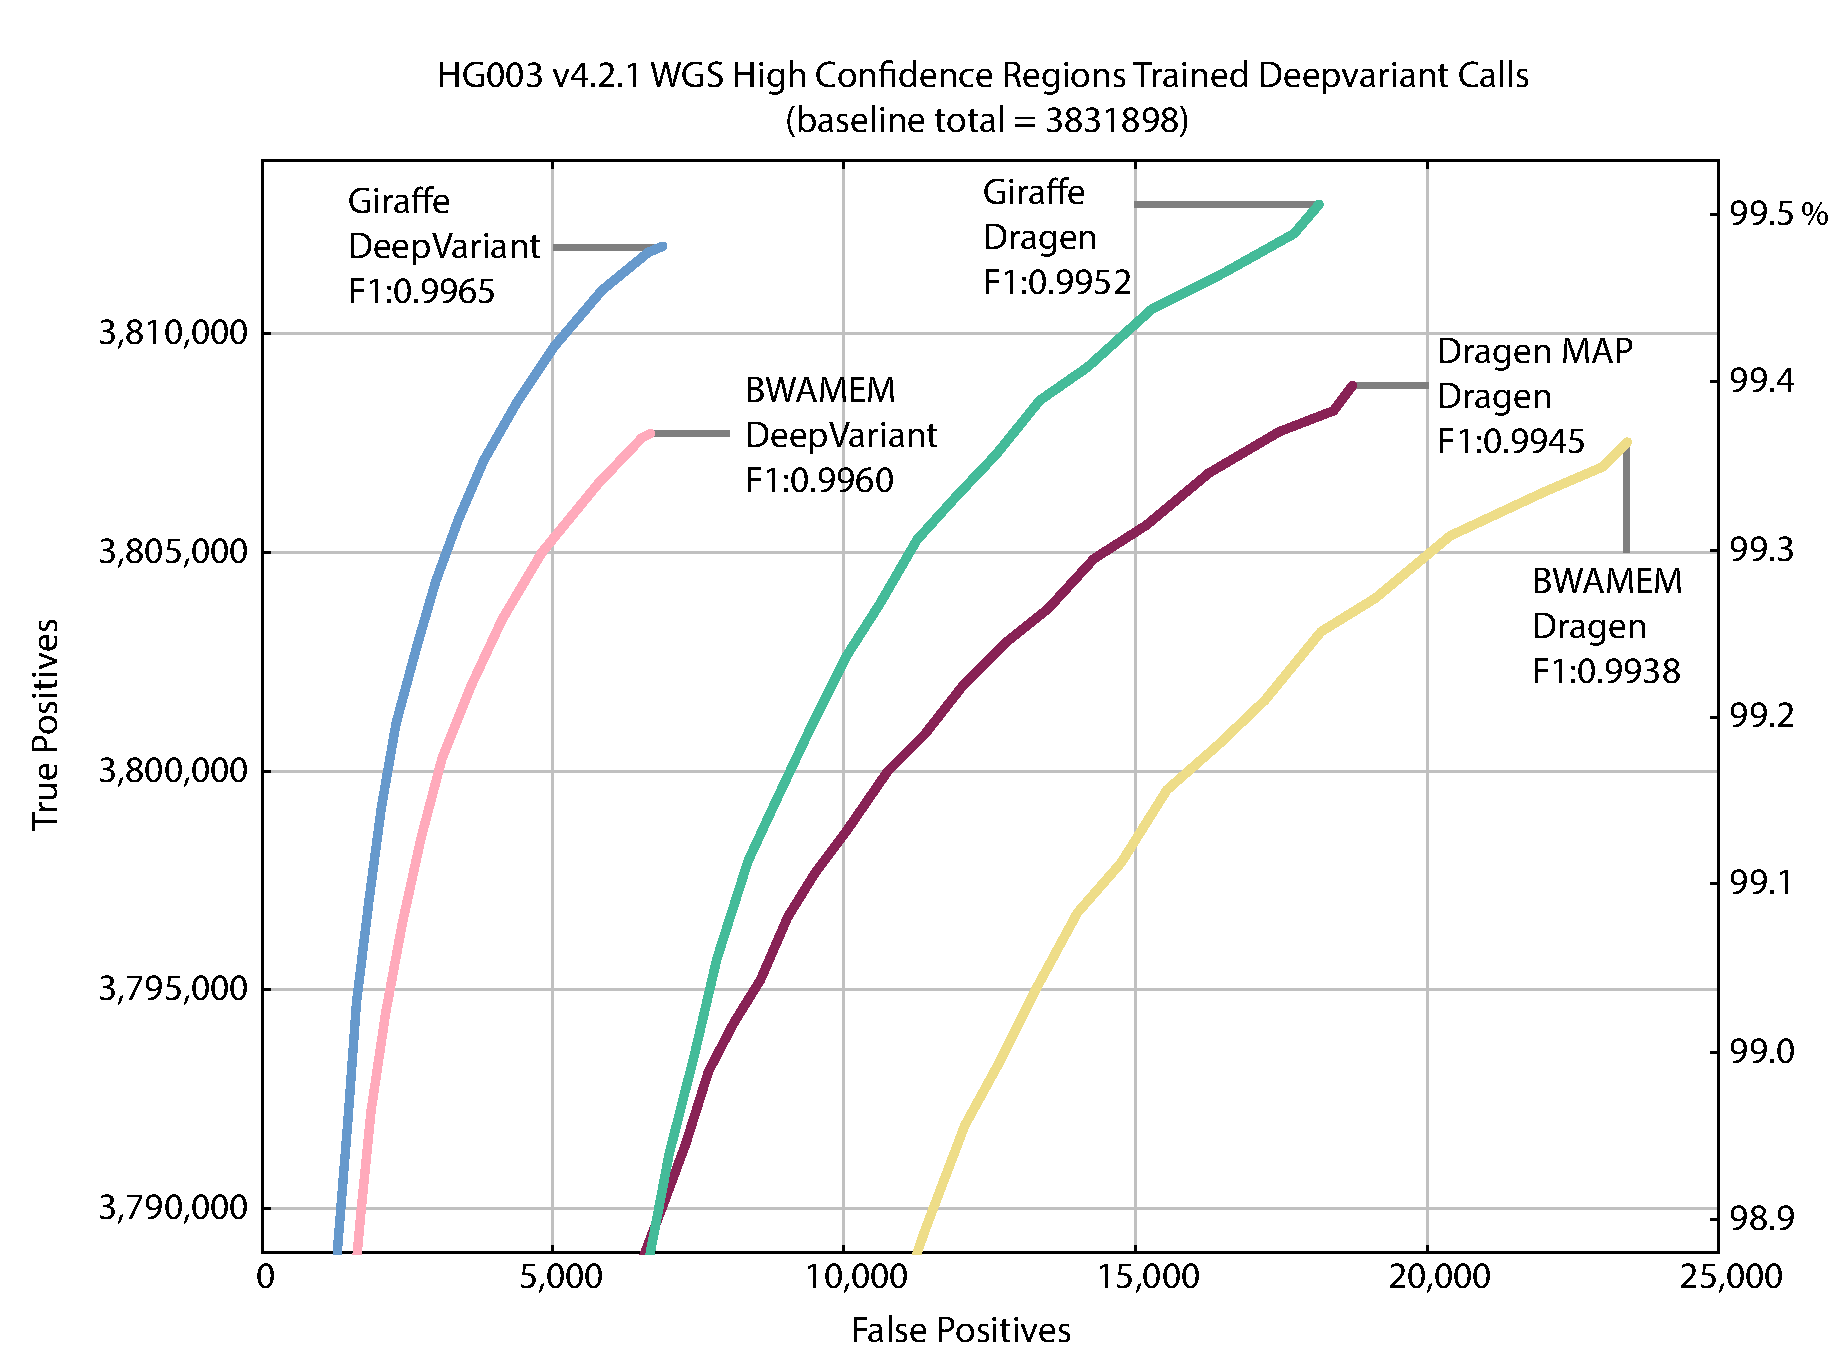
\includegraphics[width=\linewidth]{HG003_trained_deepvariant_genotyping.pdf}
    \caption[Genotyping evaluation for the DeepVariant genotyper with projected mappings from Giraffe and other mappers]{True positive and false positive genotypes made using the DeepVariant genotyper trained on alignments of 150bp paired-end reads from HG002 and HG004 GIAB samples and tested on 150bp paired-end reads from the HG003 GIAB sample and evaluated against the HG003 GIAB v4.2.1 truth variant call sets in high confidence regions. Dragen genotyper results are included for performance comparison. The ROC curve discrimination threshold is based on variant call quality.}
    \label{fig:trained_deepvariant_genotyping}
\end{figure}

\begin{figure}[H]
    \centering
    \includegraphics[width=.9\linewidth, page=2]{fig-sveval.pdf}
    \caption[SV evaluation of vg and GraphTyper on HGSVC and GIAB]{{\bf SV evaluation of vg and GraphTyper on HGSVC and GIAB.}
      SV were genotyped with vg and GraphTyper and compared to the truthset from HGSVC\cite{chaisson_sv_2019} and GIAB\cite{zook_robust_2020}.
      When genotyping the HGSVC catalog, we used short-reads from the three individuals and one set of simulated reads for one individual.
      When genotyping the GIAB catalog, we genotyped SV from short-read for HG002.
      The y-axis shows the F1 score when assessing the presence/absence of a SV (semi-transparent bars) or exact genotype (opaque bars), for vg (red) and GraphTyper (blue).
      GraphTyper outputs multiple entries for the same variant which decreases the genotyping accuracy when including all the variants (light blue).
      To improve the genotyping performance, we selected one prediction per variant for GraphTyper (darker blue).
      Finally, insertions and deletions were evaluated separately (top vs bottom) on the whole genome or high-confidence regions (x-axis).
      Panels A, B, and C show the F1 score, precision, and recall, respectively.
      }
    \label{fig:graphtyper_eval}
\end{figure}

\begin{figure}[H]
    \centering
    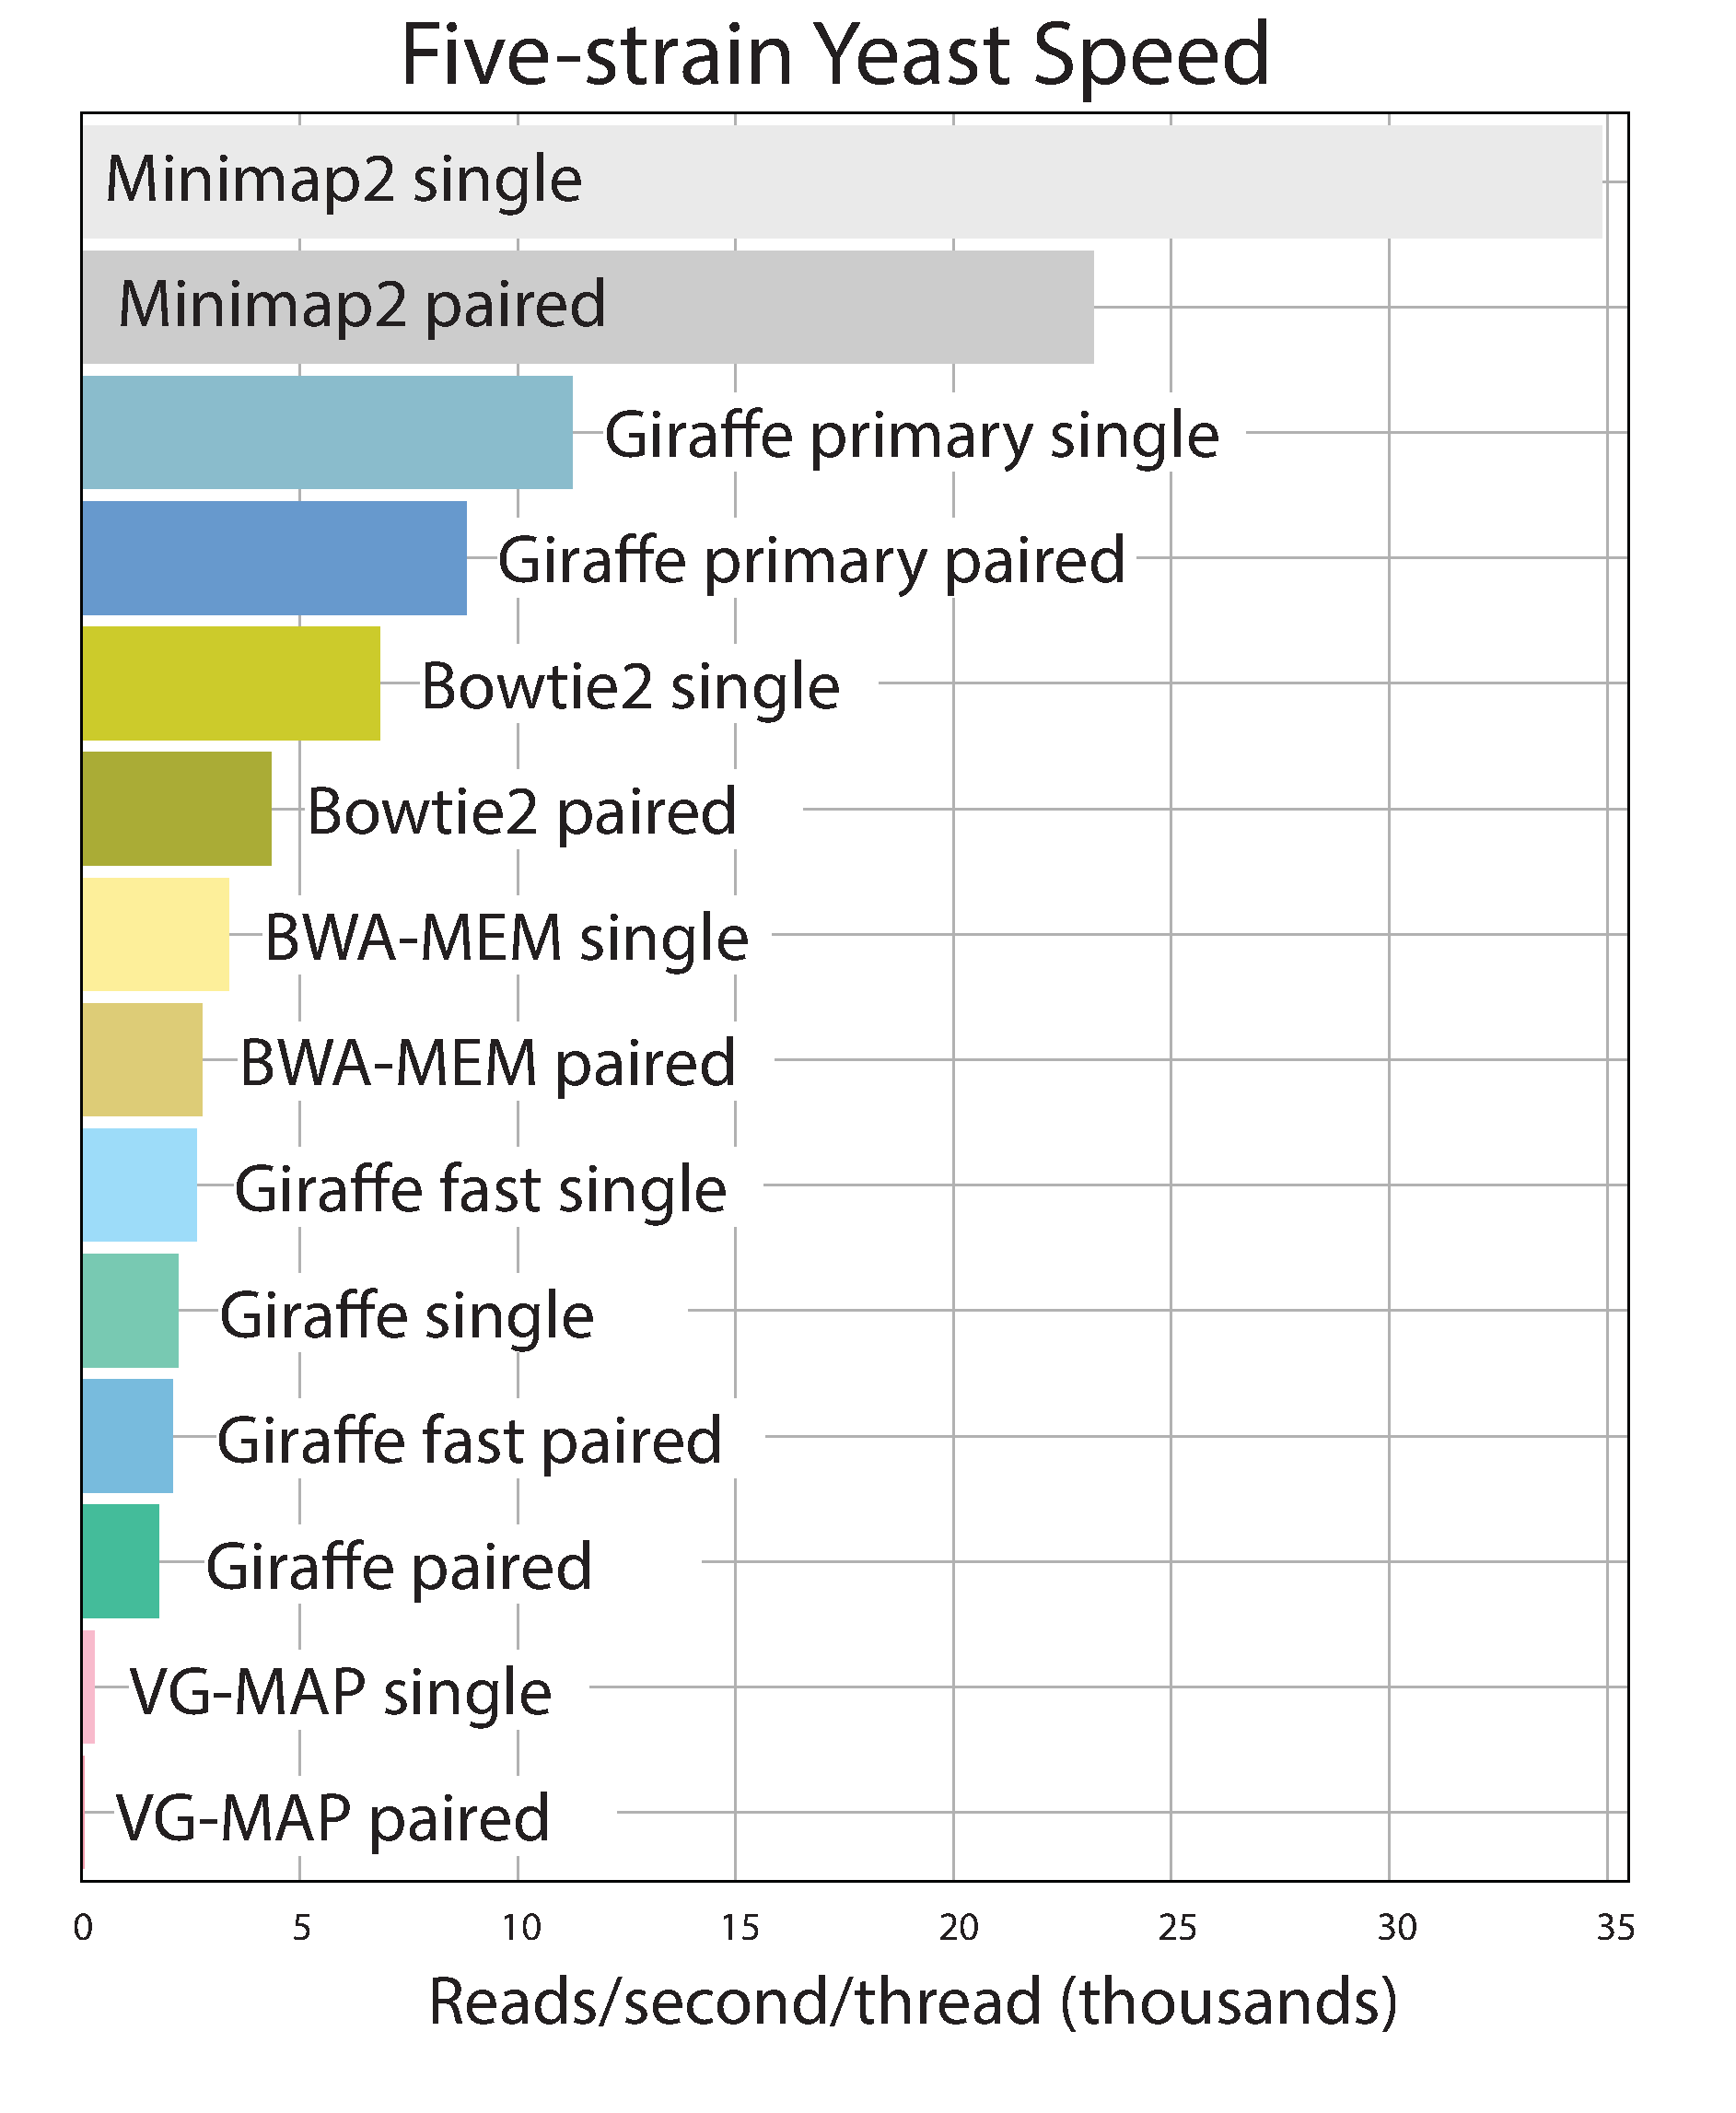
\includegraphics[width=.7\linewidth]{speed_yeast.pdf}
    \caption[Mapping speed on yeast data]{\textbf{Mapping speed on yeast data.} Each mapper was run on a dataset of 1 million real HiSeq 2500 reads from the DBVPG6044 strain on an AWS EC2 i3.8xlarge node with 32 vCPUs and 244GB of memory. The speed of mapping in reads per second per thread was determined using the total time spend mapping as reported by each tool. Each tool except Minimap2 was run on 16 threads; Minimap2 was run on 2 threads because it did not use all 16 threads.}
    \label{fig:speed_yeast}
\end{figure}

\begin{figure}[htp]
    \centering
    \includegraphics[width=.9\linewidth]{aim2_supplement_wdl-sveval.pdf}
    \caption[Structural variant genotyping workflow]{\textbf{Structural variant genotyping workflow.}
      (A, B, C) SV genotyping F1, precision, and recall (respectively) for the SV graph combining HGSVC \cite{chaisson_sv_2019}, SVPOP \cite{audano_hgsvc} and GIAB \cite{zook_robust_2020}, and for individual SV graphs containing only HGSVC or GIAB as used in Hickey et al.\cite{hickey_vgsv_2020}.
      The genotypes predicted from the long-read sequencing data in the original studies are used as truthset.
      (D) Workflow overview with average resources used for each task for a typical sample (Table \ref{tab:svwdl-task}). Note: the core hours estimates include the time spent copying files between computing instances.
    }
    \label{fig:sv-wdl-graph}
\end{figure}


\begin{figure}[H]
    \centering
    \includegraphics[width=.9\linewidth, page=1]{fig-sveval.pdf}
    \caption[Minimal effect of down-sampling reads to 20x depth on the SV genotyping performance]{{\bf Minimal effect of down-sampling reads to 20x depth on the SV genotyping performance.}
      HG00514 was genotyped using the SV graph combining HGSVC, SVPOP and GIAB.
      Panels A, B, and C show the F1 score, precision, and recall, respectively.
    }
    \label{fig:sveval-depth}
\end{figure}



\begin{figure}[H]
    \centering
    \includegraphics[width=.9\linewidth]{fig-sv-mesa-stats-2.pdf}
    \caption[SV alleles and SV sites in the MESA cohort]{{\bf SV alleles and SV sites in the MESA cohort.}
      (A) Proportion of SV loci in clique formation, i.e. with alleles different by only small variants (SNVs, indels) as opposed to large allelic variation such as VNTRs.
      The more alleles in a SV site the more likely it is to show VNTR-like allelic patterns.
      (B) Fold-change between the major allele and the second most frequent allele in a SV loci (y-axis), grouped by the number of alleles in the locus (x-axis).
      The number of loci with a fold-change higher than 3 (dotted line) are labeled.
    }
    \label{fig:svsites_mesa}
\end{figure}


\begin{figure}[H]
  \centering
  %~~~(A)\hfill{(B)~~~}

  %\includegraphics[width=.49\linewidth, page=1]{examples-svsites-mesa.pdf}
  %\includegraphics[width=.49\linewidth, page=2]{examples-svsites-mesa.pdf}

  %~~~(C)\hfill{(D)~~~}

  %\includegraphics[width=.49\linewidth, page=3]{examples-svsites-mesa.pdf}
  %\includegraphics[width=.49\linewidth, page=4]{examples-svsites-mesa.pdf}
  \includegraphics[width=\linewidth]{examples-svsites-mesa-all.pdf}
  \caption[Four examples of SV sites in the MESA cohort]{{\bf Four examples of SV sites in the MESA cohort.}
    For each site, the top left panel shows a representation of their configuration in the genomic region, the top right panel shows the distribution of allele frequencies across the 2000 MESA samples, and the bottom panel shows the result of a multiple-sequence alignment of the inserted/deleted sequences.
    In (A) and (B), the insertions' alleles are only different due to small variants while (C) and (D) shows an insertion and deletion site with significant size variation between the alleles.
    In (A), there is one major allele while multiple alleles of (B) are frequent in the population. }
  \label{fig:mesa-svsite-examples}
\end{figure}


\begin{figure}[H]
    \centering
    \includegraphics[width=\linewidth]{fig-sv-1kgp-stats.pdf}
    \caption[Structural variants in 2,504 unrelated individuals from the 1000 Genomes Project]{\textbf{Structural variants in 2,504 unrelated individuals from the 1000 Genomes Project.}
      (A) Allele frequency distribution of the major allele for each SV loci.
      (B) Size distribution of the major allele for each SV loci.
      (C) Cumulative proportion of SV loci depending on the maximum number of alleles (x-axis) in the locus.
      (D) Proportion of SV loci in clique formation, i.e. with alleles different by only small variants (SNVs, indels) as opposed to large allelic variation such as VNTRs.
      The more alleles in a SV site the more likely it is to show VNTR-like allelic patterns.
      (E) Fold-change between the major allele and the second most frequent allele in a SV loci (y-axis), grouped by the number of alleles in the locus (x-axis).
      The number of loci with a fold-change higher than 3 (dotted line) are labeled.
    }
    \label{fig:sv-1kgp-stats}
\end{figure}

\begin{figure}[H]
  \includegraphics[width=\linewidth]{fig-sv-trio-eval.pdf}
  \caption[SV evaluation using 602 trios from the 1000 Genomes Project]{{\bf SV evaluation using 602 trios from the 1000 Genomes Project}
    (A) Mendelian error (y-axis) for different minimum genotype quality thresholds (x-axis), i.e. considering all variants where the minimum genotype quality in the trio is X or higher.
    (B) Proportion of transmitted allele from an heterozygous parent (y-axis) for the same minimum genotype quality thresholds (x-axis).
    In (A) and (B), the vertical lines represent the full error range across all trios while the point represents the median error.
    (C) Proportion of variants (y-axis) passing each minimum genotype quality threshold (x-axis).
  }
  \label{fig:sv-trio-eval}
\end{figure}


\begin{figure}[H]
  \includegraphics[width=\linewidth]{fig-sv-freq-comp.pdf}
  \caption[Allele frequency of SVs in this study and public studies]{{\bf Allele frequency of SVs in this study and public studies.}
    (A) Allele frequency distribution of common variants (frequency >1\%) in each dataset.
    (B-D) show the difference in frequency between our results in the MESA cohort and each of the three public catalogs (1000 Genome Project phase 3, gnomAD-SV, SVPOP).
    (E-F) show the difference in frequency between SVPOP and the two other public catalogs.}
  \label{fig:sv-freq-comp}
\end{figure}

\begin{figure}[H]
  \includegraphics[width=\linewidth, page=3]{fig-sv-mesa-pcs.pdf}
  \caption[Principal component analysis using the SV genotypes or SNVs in the MESA dataset]{{\bf Principal component analysis using the SV genotypes (y-axis) in the MESA dataset compared to the principal components derived from TOPMed-wide SNVs (x-axis).}
    (A), (B), (C) compare the first, second and third components.}
  \label{fig:mesa-topmed-pcs}
\end{figure}


\begin{figure}[H]
  \includegraphics[width=\linewidth]{fig-pops-freq-mesa.pdf}
  \caption[SV sites with population specific frequency patterns in the MESA cohort]{{\bf SV sites with population specific frequency patterns in the MESA cohort.}
    The two thousand MESA samples were clustered in 6 clusters based on the top 3 principal components (A-B).
    (C) The range of frequency, i.e. the difference between the maximum and minimum frequencies, across the sample clusters was larger than expected (permutation) for thousands of SV sites.
    (D) Two clusters (x-axis) show high number of population-specific SV sites (y-axis), defined as deviating from the median allele frequency by at least 10\%, 25\%, or 50\% (panels).}
  \label{fig:mesa-pop-freq}
\end{figure}

\begin{figure}[H]
  \includegraphics[width=\linewidth]{fig-sv-1kgp-pcs.pdf}
  \caption[PCA of SV genotypes in the 1000 Genomes Project]{{\bf Principal component analysis from structural variant genotypes across the 2,504 unrelated individuals in the 1000 Genomes Project dataset. }
    Principal component analysis was performed on the SV genotypes predicted by vg across the 166,199 SV loci.
    Individuals are colored according to their assigned ``super population'' in the 1000 Genomes Project.
    (A) shows the first and second principal components, (B) shows the third and fourth components.
  }
  \label{fig:1kgp-sv-pcs}
\end{figure}
\newpage

\begin{figure}[H]
  \includegraphics[width=\linewidth]{fig-pops-freq-kgp.pdf}
  \caption[SV sites with population specific frequency patterns in the 2,504 individuals from the 1000 Genomes Project]{{\bf SV sites with population specific frequency patterns in the 2,504 individuals from the 1000 Genomes Project. }
    (A) The range of frequency, i.e. the difference between the maximum and minimum frequencies, across the super-population was larger than expected (permutation) for thousands of SV sites.
    (B) Super-populations (x-axis) show high number of population-specific SV sites (y-axis), defined as deviating from the median allele frequency by at least 10\%, 25\%, or 50\% (panels).}
  \label{fig:1kgp-pop-freq}
\end{figure}


\begin{figure}[H]
  \includegraphics[width=\linewidth]{fig-sv-eqtl.pdf}
  \caption[P-value distribution of the SV vs gene expression tests in the GEUVADIS dataset]{{\bf P-value distribution of the SV vs gene expression tests in the GEUVADIS dataset.}
    Three analysis were performed: joint European and Yoruba populations (A-B), European populations only (C-D), and the Yoruba population (YRI) only (E-F).
    (A,C,E) show the p-value distribution, uniform except for the peak of low p-values.
    (B,D,F) show the QQ plots for the three analysis.
  }
  \label{fig:eqtl_qc}
  \end{figure}

\begin{figure}[H]
  \includegraphics[width=\linewidth, page=2]{fig-sv-functional-summary.pdf}
  \caption[Location of the SV-eQTLs around the associated gene]{{\bf Location of the SV-eQTLs around the associated gene}
    The x-axis reports the proportion of SV-eQTLs overlapping each annotation group (panels).
    A SV-eQTL is either positively (red) or negatively (blue) associated with gene expression, i.e. each additional SV allele correlates with increased or decreased gene expression respectively.
    The control bar (green) represents the expected distribution of common SVs around control genes.
    Control genes were chosen to match the size distribution of genes involved in eQTLs.
    {\it UTR: untranslated region.}
  }
  \label{fig:eqtl_enr}
\end{figure}

\begin{figure}[H]
  \includegraphics[width=\linewidth, page=1]{fig-sv-snv-indel-eqtl.pdf}
  \caption[Enrichment of SV-eQTLs in highly expressed genes]{{\bf Enrichment of SV-eQTLs in highly expressed genes}
    Genes were split in 20 expression groups of equal size (quantiles).
    The graph shows the proportion of eQTLs (y-axis) in each expression quantile (x-axis).
    We see a strong enrichment for SV-eQTLs (blue) in the last quantile representing the mist expressed genes.
    The enrichment is also significant (point size) if only weaker for SNV/indel eQTLs.
    The horizontal dotted line represents the expected value, i.e. 1/20 of the eQTLs in each quantile group.
  }
  \label{fig:eqtl_enr_ge}
\end{figure}

\begin{figure}[H]
  \textsf{(A)} \hspace{15em} \textsf{(B)}

  \includegraphics[trim={0 0em 0 20em}, clip, width=\linewidth, page=2]{fig-sv-snv-indel-eqtl.pdf}
  \caption[Example of a SV lead-eQTL]{{\bf Example of SV lead-eQTL}
    Association between an intronic 5,405 bp deletion and the gene expression of the {\it SLC44A5} gene.
    (A) Each additional allele is associated with a decrease in gene expression.
    (B) shows the position of significant eQTLs (SNV/indels in green, deletion in red, insertion in blue).
    The y-axis represents the significance of the association, with the top eQTL being the highest point.
    The deletion is the most significant eQTLs and the significance decreases the farther the variant is from it.
  }
  \label{fig:eqtl_ex}
\end{figure}

\begin{figure}[H]
    \centering
    \includegraphics[width=.7\linewidth]{aim2_supplement_speed.pdf}
    \caption[Mapping speed on human data]{\textbf{Mapping speed on human data.} Each mapper was run on a dataset of 1 million real NovaSeq 6000 (A,B), HiSeq X Ten (C,D), or HiSeq 2500 (E,F) reads on a AWS EC2 i3.8xlarge node with 32 vCPUs and 244GB of memory. The speed of mapping in reads per second per thread was determined using the total time spend mapping as reported by each tool. Each tool except Minimap2 was run on 16 threads; Minimap2 was run on 2 threads because it did not use all 16 threads.}
    \label{fig:aim2_supplement_speed}
\end{figure}


\begin{figure}[H]
    \includegraphics[width=.5\linewidth]{aim2_supplement_regiondiagram.pdf}
    \caption[Diagram of minimizers, agglomerations, and regions]{{\bf Diagram of minimizers, agglomerations, and regions.} In this example, we use a minimizer length of $k=3$, and a window size of $w=4$. (A) shows where three example minimizers fall in the read. (B) shows the agglomerations of these minimizers, if the minimizers happen to be minimal for all windows they appear in. For agglomeration $i=1$, we have $\aggstart{1}=1$, $\aggend{1}=5$, $\minstart{1}=2$, and $\minend{1}=4$. (C) shows the regions, which we use to decompose the part of the diagram covered by agglomerations, with breaks wherever an agglomeration begins or ends. For the region $r=3$, we have $\rtop{3}=1$, $\rbottom{3}=2$, $\rleft{3}=4$, and $\rright{3}=5$.
  }
  \label{fig:aim2_supplement_regions}
\end{figure}

\section{Supplementary tables}


\newcommand{\mapindexes}[1]{\indexurl{#1.xg} & \indexurl{#1.gcsa} & \indexurl{#1.gcsa.lcp} & & & &}
\newcommand{\giraffeindexes}[1]{\indexurl{#1.xg} & & & \indexurl{#1.gbwt} & \indexurl{#1.min} & \indexurl{#1.gg} & \indexurl{#1.dist}}

\begin{table}[H]
    \centering
    \begin{tabular}{|l|l|r|r|r|}
    \hline
        Pairing & Mapper & \% Correct & \% MAPQ 60 & \% Incorrect and  \\
              &         &            &            & MAPQ 60           \\
        \hline
        single  & Giraffe primary	    & 96.94     & 91.81     & 0.00195 \\
                & VG-MAP primary        & 97.03     & 92.16     & 0.00125 \\
                & Bowtie2	            & 96.84     & 82.85     & 0.00075 \\
                & BWA-MEM	            & 97.05     & 91.07     & 0.00085 \\
                & Minimap2	            & 96.82     & 90.32     & 0.00250 \\
                & Giraffe	            & 97.00     & 92.29     & 0.00040 \\
                & fast Giraffe	        & 96.86     & 89.82     & 0.00075 \\
                & VG-MAP               	& 96.99     & 91.90     & 0.00005 \\
                & GraphAligner	        & 88.95     & -         & - \\
                & HISAT2	            & 96.69     & 95.83     & 0.20275 \\
                & HISAT2 sens       	& 96.76     & 95.92     & 0.22765 \\
                & HISAT2 vsens	        & 96.83     & 96.00     & 0.25985 \\
                & Giraffe control	    & 97.12     & 93.14     & 0.00020 \\

        \hline
        paired  & Giraffe Primary	& 98.25     & 94.22     & 0.00135 \\
                & VG-MAP Primary	& 98.28     & 94.47     & 0.00140 \\
                & Bowtie2       	& 98.25     & 88.75     & 0.00150 \\
                & BWA-MEM	        & 98.33     & 93.95     & 0.00120 \\
                & Minimap2      	& 98.01     & 93.25     & 0.02710 \\
                & Giraffe	        & 98.27     & 94.34     & 0.00015 \\
                & fast Giraffe  	& 98.24     & 92.84     & 0.00015 \\
                & VG-MAP           	& 98.29     & 94.41     & 0.00050 \\
                & HISAT2        	& 97.95     & 97.50     & 0.31180 \\
                & HISAT2 sens   	& 98.11     & 97.73     & 0.38640 \\
                & HISAT2 vsens	    & 98.18     & 97.66     & 0.27780 \\
                & Giraffe control	& 98.33     & 94.70     & 0.00000 \\
 
 
        \hline
        
    \end{tabular}
    \caption[Mapping accuracy on NovaSeq 6000 reads mapped to the 1000GP graph/GRCh38 reference]{\textbf{Mapping accuracy on NovaSeq 6000 reads mapped to the 1000GP graph/GRCh38 reference} Each mapper was run on 2 million simulated reads and assessed for the percent of reads that were mapped correctly, the percent of reads that were assigned mapping quality 60, and the percent of reads that were incorrect and assigned mapping quality 60. *Bowtie2 had a maximum mapping quality of 42. GraphAligner did not assign mapping quality}
    \label{tab:mapping_accuracy_1kg_novaseq6000}
    \label{tab:first}
\end{table}

\begin{table}[H]
    \centering
    \begin{tabular}{|l|l|r|r|r|}
    \hline
        Pairing & Mapper & \% Correct & \% MAPQ 60 & \% Incorrect and \\
               &         &            &            & MAPQ 60          \\
        \hline
        single  & Giraffe primary	& 96.93     & 91.68     & 0.00260 \\
                & VG-MAP primary	& 97.04     & 92.17     & 0.00085 \\
                & Bowtie2       	& 96.75     & 83.73     & 0.00185 \\
                & BWA-MEM	        & 97.03     & 91.06     & 0.00050 \\
                & Minimap2	        & 96.80     & 90.28     & 0.00200 \\
                & Giraffe	        & 97.00     & 92.19     & 0.00080 \\
                & fast Giraffe	    & 96.83     & 90.02     & 0.00095 \\
                & VG-MAP	        & 97.00     & 91.92     & 0.00020 \\
                & GraphAligner 	    & 88.82     & -         & - \\
                & HISAT2	        & 96.51     & 95.75     & 0.30710 \\
                & HISAT2 sens	    & 96.62     & 95.89     & 0.33675 \\
                & HISAT2 vsens  	& 96.71     & 95.93     & 0.32535 \\
                & Giraffe control	& 97.11     & 93.04     & 0.00020 \\

        \hline
        paired  & Giraffe primary	& 98.27     & 94.27     & 0.00155 \\
                & VG-MAP primary   	& 98.29     & 94.48     & 0.00125 \\
                & Bowtie2       	& 98.21     & 89.07     & 0.00245 \\
                & BWA-MEM	        & 98.33     & 93.94     & 0.00095 \\
                & Minimap2	        & 98.00     & 93.23     & 0.02785 \\
                & Giraffe	        & 98.28     & 94.40     & 0.00025 \\
                & fast Giraffe	    & 98.24     & 93.13     & 0.00010 \\
                & VG-MAP	        & 98.30     & 94.41     & 0.00060 \\
                & HISAT2        	& 97.71     & 97.33     & 0.37060 \\
                & HISAT2 sens   	& 97.95     & 97.66     & 0.45725 \\
                & HISAT2 vsens	    & 98.12     & 97.68     & 0.33825 \\
                & Giraffe control	& 98.35     & 94.72     & 0.00010 \\
        \hline
        
    \end{tabular}
    \caption[Mapping accuracy on HiSeq X Ten reads mapped to the 1000GP graph/GRCh38 reference]{\textbf{Mapping accuracy on HiSeq X Ten reads mapped to the 1000GP graph/GRCh38 reference} Each mapper was run on 2 million simulated reads and assessed for the percent of reads that were mapped correctly, the percent of reads that were assigned mapping quality 60, and the percent of reads that were incorrect and assigned mapping quality 60. *Bowtie2 had a maximum mapping quality of 42. GraphAligner did not assign mapping quality}
    \label{tab:mapping_accuracy_1kg_hiseqxten}
\end{table}

\begin{table}[H]
    \centering
    \begin{tabular}{|l|l|r|r|r|}
    \hline
        Pairing & Mapper & \% Correct & \% MAPQ 60 & \% Incorrect and \\
               &         &            &            & MAPQ 60          \\
        \hline
        single  & Giraffe primary	& 97.80     & 94.95     & 0.00530 \\
                & VG-MAP primary	& 97.90     & 93.99     & 0.00200 \\
                & Bowtie2	        & 96.48     & 84.41     & 0.00435 \\
                & BWA-MEM       	& 97.84     & 92.61     & 0.05120 \\
                & Minimap2      	& 97.69     & 93.17     & 0.05120 \\
                & Giraffe       	& 97.84     & 95.04     & 0.00295 \\
                & fast Giraffe	    & 97.72     & 94.06     & 0.00285 \\
                & VG-MAP           	& 97.90     & 93.90     & 0.00115 \\
                & GraphAligner 	    & 92.93     & -         & - \\
                & HISAT2        	& 94.94     & 95.03     & 0.72205 \\
                & HISAT2 sens	    & 96.03     & 96.01     & 0.67535 \\
                & HISAT2 vsens  	& 96.41     & 96.11     & 0.51385 \\
                & Giraffe control	& 97.94     & 95.27     & 0.00110 \\

        \hline
        paired  & Giraffe primary	& 98.68     & 95.84     & 0.00350 \\
                & VG-MAP primary   	& 98.76     & 95.67     & 0.00225 \\
                & Bowtie2	        & 97.30     & 87.87     & 0.00715 \\
                & BWA-MEM       	& 98.71     & 94.64     & 0.05415 \\
                & Minimap2      	& 98.39     & 92.68     & 0.08915 \\
                & Giraffe	        & 98.69     & 95.87     & 0.00205 \\
                & fast Giraffe  	& 98.65     & 95.25     & 0.00180 \\
                & VG-MAP	        & 98.76     & 95.66     & 0.00130 \\
                & HISAT2        	& 95.52     & 95.80     & 0.78575 \\
                & HISAT2 sens	    & 96.84     & 97.16     & 0.81925 \\
                & HISAT2 vsens	    & 97.32     & 97.27     & 0.56045 \\
                & Giraffe control	& 98.78     & 95.91     & 0.00145 \\

        \hline
        
    \end{tabular}
    \caption[Mapping accuracy on HiSeq 2500 reads mapped to the 1000GP graph/GRCh38 reference]{\textbf{Mapping accuracy on HiSeq 2500 mapped to the 1000GP graph/GRCh38 reference} Each mapper was run on 2 million simulated reads and assessed for the percent of reads that were mapped correctly, the percent of reads that were assigned mapping quality 60, and the percent of reads that were incorrect and assigned mapping quality 60. *Bowtie2 had a maximum mapping quality of 42. GraphAligner did not assign mapping quality}
    \label{tab:mapping_accuracy_1kg_hiseq2500}
\end{table}

\begin{table}[H]
    \centering
    \begin{tabular}{|l|l|r|r|r|}
    \hline
        Pairing & Mapper & \% Correct & \% MAPQ 60 & \% Incorrect and\\
               &         &            &            & MAPQ 60          \\
        \hline
        single  & Giraffe primary	& 97.09     & 92.68     & 0.04840 \\
                & VG-MAP primary   	& 97.17     & 92.62     & 0.04685 \\
                & Bowtie2	        & 97.02     & 84.20     & 0.02645 \\
                & BWA-MEM	        & 97.16     & 91.61     & 0.03925 \\
                & Minimap2	        & 96.96     & 90.93     & 0.04220 \\
                & Giraffe	        & 97.17     & 92.63     & 0.00070 \\
                & fast Giraffe	    & 97.02     & 90.25     & 0.00070 \\
                & VG-MAP	        & 97.24     & 92.57     & 0.00035 \\
                & GraphAligner 	    & 91.94     & -      & - \\
                & HISAT2	        & 97.10     & 96.36     & 0.20975 \\
                & HISAT2 sens   	& 97.16     & 96.46     & 0.24702 \\
                & HISAT2 vsens	    & 97.24     & 96.58     & 0.30368 \\
                & Giraffe control	& 97.26     & 93.42     & 0.00005 \\

        \hline
        paired  & Giraffe primary	& 98.29     & 94.65     & 0.05480 \\
                & HISAT2	        & 96.51     & 95.75     & 0.30710 \\
                & Bowtie2       	& 98.28     & 89.54     & 0.03220 \\
                & BWA-MEM       	& 98.38     & 94.34     & 0.04275 \\
                & Minimap2      	& 98.09     & 93.72     & 0.06800 \\
                & Giraffe       	& 98.39     & 94.57     & 0.00040 \\
                & fast Giraffe  	& 98.35     & 93.14     & 0.00040 \\
                & VG-MAP	        & 98.41     & 94.74     & 0.00385 \\
                & HISAT2	        & 98.24     & 97.95     & 0.35377 \\
                & HISAT2 sens   	& 98.36     & 98.17     & 0.44951 \\
                & HISAT2 vsens	    & 98.41     & 98.16     & 0.39059 \\
                & Giraffe control	& 98.47     & 94.96     & 0.00005 \\

        \hline
        
    \end{tabular}
    \caption[Mapping accuracy on NovaSeq 6000 reads mapped to the HGSVC graph/GRCh38 reference]{\textbf{Mapping accuracy on NovaSeq 6000 reads mapped to the HGSVC graph/GRCh38 reference} Each mapper was run on 2 million simulated reads and assessed for the percent of reads that were mapped correctly, the percent of reads that were assigned mapping quality 60, and the percent of reads that were incorrect and assigned mapping quality 60. *Bowtie2 had a maximum mapping quality of 42. GraphAligner did not assign mapping quality}
    \label{tab:mapping_accuracy_hgsvc_novaseq6000}
\end{table}

\begin{table}[H]
    \centering
    \begin{tabular}{|l|l|r|r|r|}
    \hline
        Pairing & Mapper & \% Correct & \% MAPQ 60 & \% Incorrect and \\
               &         &            &            & MAPQ 60          \\
        \hline
        single  & Giraffe primary	& 97.10     & 92.57     & 0.04850 \\
                & VG-MAP primary   	& 97.20     & 92.63     & 0.04585 \\
                & Bowtie2       	& 96.94     & 85.15     & 0.02865 \\
                & BWA-MEM       	& 97.19     & 91.61     & 0.03885 \\
                & Minimap2	        & 96.96     & 90.86     & 0.04140 \\
                & Giraffe	        & 97.16     & 92.52     & 0.00100 \\
                & fast Giraffe  	& 97.01     & 90.43     & 0.00130 \\
                & VG-MAP	        & 97.27     & 92.58     & 0.00035 \\
                & GraphAligner   	& 91.88     & -         & - \\
                & HISAT2	        & 96.92     & 96.32     & 0.30077 \\
                & HISAT2 sens   	& 97.02     & 96.45     & 0.34180 \\
                & HISAT2 vsens	    & 97.11     & 96.52     & 0.34185 \\
                & Giraffe control	& 97.27     & 93.34     & 0.00015 \\

        \hline
        paired  & Giraffe primary	& 98.29     & 94.76     & 0.05470 \\
                & VG-MAP primary   	& 98.35     & 94.84     & 0.04750 \\
                & Bowtie2       	& 98.25     & 89.98     & 0.03325 \\
                & BWA-MEM        	& 98.40     & 94.36     & 0.04280 \\
                & Minimap2      	& 98.07     & 93.69     & 0.06815 \\
                & Giraffe	        & 98.38     & 94.68     & 0.00050 \\
                & fast Giraffe	    & 98.34     & 93.43     & 0.00030 \\
                & VG-MAP           	& 98.43     & 94.79     & 0.00420 \\
                & HISAT2	        & 98.04     & 97.82     & 0.40337 \\
                & HISAT2 sens   	& 98.23     & 98.13     & 0.51313 \\
                & HISAT2 vsens	    & 98.36     & 98.16     & 0.42937 \\
                & Giraffe control	& 98.48     & 95.01     & 0.00005 \\
        \hline
        
    \end{tabular}
    \caption[Mapping accuracy on HiSeq X Ten reads mapped to the HGSVC graph/GRCh38 reference]{\textbf{Mapping accuracy on HiSeq X Ten reads mapped to the HGSVC graph/GRCh38 reference} Each mapper was run on 2 million simulated reads and assessed for the percent of reads that were mapped correctly, the percent of reads that were assigned mapping quality 60, and the percent of reads that were incorrect and assigned mapping quality 60. *Bowtie2 had a maximum mapping quality of 42. GraphAligner did not assign mapping quality}
    \label{tab:mapping_accuracy_hgsvc_hiseqxten}
\end{table}

\begin{table}[H]
    \centering
    \begin{tabular}{|l|l|r|r|r|}
    \hline
        Pairing & Mapper & \% Correct & \% MAPQ 60 & \% Incorrect and \\
               &         &            &            & MAPQ 60          \\
        \hline
        single  & Giraffe primary	& 97.89     & 95.34     & 0.06980 \\
                & VG-MAP primary	& 97.98     & 94.38     & 0.05715 \\
                & Bowtie2	        & 96.56     & 85.74     & 0.03405 \\
                & BWA-MEM	        & 97.93     & 93.08     & 0.09025 \\
                & Minimap2	        & 97.78     & 93.59     & 0.09525 \\
                & Giraffe	        & 97.97     & 95.30     & 0.00430 \\
                & fast Giraffe	    & 97.87     & 94.35     & 0.00340 \\
                & VG-MAP           	& 98.08     & 94.35     & 0.00170 \\
                & GraphAligner 	    & 94.86     & -         & -0 \\
                & HISAT2	        & 95.32     & 95.47     & 0.69207 \\
                & HISAT2 sens   	& 96.36     & 96.41     & 0.66196 \\
                & HISAT2 vsens  	& 96.73     & 96.58     & 0.54163 \\
                & Giraffe control	& 98.07     & 95.53     & 0.00075 \\

        \hline
        paired  & Giraffe primary	& 98.70     & 96.10     & 0.06465 \\
                & VG-MAP primary	& 98.79     & 95.93     & 0.05845 \\
                & Bowtie2       	& 97.33     & 88.71     & 0.03860 \\
                & BWA-MEM       	& 98.75     & 94.97     & 0.09730 \\
                & Minimap2      	& 98.44     & 93.02     & 0.12805 \\
                & Giraffe       	& 98.80     & 96.04     & 0.00295 \\
                & fast Giraffe  	& 98.78     & 95.44     & 0.00280 \\
                & VG-MAP        	& 98.89     & 95.89     & 0.00280 \\
                & HISAT2        	& 95.86     & 96.18     & 0.75739 \\
                & HISAT2 sens   	& 97.09     & 97.51     & 0.82688 \\
                & HISAT2 vsens	    & 97.55     & 97.72     & 0.63802 \\
                & Giraffe control	& 98.91     & 96.13     & 0.00165 \\


        \hline
        
    \end{tabular}
    \caption[Mapping accuracy on HiSeq 2500 reads mapped to the HGSVC graph/GRCh38 reference]{\textbf{Mapping accuracy on HiSeq 2500 reads mapped to the HGSVC graph/GRCh38 reference} Each mapper was run on 2 million simulated reads and assessed for the percent of reads that were mapped correctly, the percent of reads that were assigned mapping quality 60, and the percent of reads that were incorrect and assigned mapping quality 60. *Bowtie2 had a maximum mapping quality of 42. GraphAligner did not assign mapping quality}
    \label{tab:mapping_accuracy_hgsvc_hiseq2500}
\end{table}

\begin{table}[H]
    \centering
    \begin{tabular}{|l|l|r|r|r|}
    \hline
        Pairing & Mapper & \% Correct & \% MAPQ 60 & \% Incorrect and \\
               &         &            &            & MAPQ 60          \\
        \hline
        single  & primary	& 97.09     & 92.68     & 0.04840 \\
                & 1x	    & 97.13     & 92.65     & 0.01840 \\
                & 2x	    & 97.15     & 92.64     & 0.01095 \\
                & 4x	    & 97.16     & 92.63     & 0.00260 \\
                & 8x	    & 97.17     & 92.63     & 0.00075 \\
                & 16x	    & 97.17     & 92.63     & 0.00070 \\
                & 32x	    & 97.17     & 92.63     & 0.00070 \\
                & 64x   	& 97.17     & 92.63     & 0.00070 \\
                & 128x	    & 97.17     & 92.63     & 0.00070 \\
                & full  	& 97.17     & 92.64     & 0.00045 \\

                
                

        \hline
        paired  & primary	& 98.29     & 94.65     & 0.05480 \\
                & 1x	    & 98.35     & 94.60     & 0.01820 \\
                & 2x	    & 98.36     & 94.59     & 0.01105 \\
                & 4x	    & 98.38     & 94.58     & 0.00240 \\
                & 8x	    & 98.38     & 94.57     & 0.00060 \\
                & 16x	    & 98.39     & 94.57     & 0.00040 \\
                & 32x	    & 98.39     & 94.57     & 0.00040 \\
                & 64x	    & 98.39     & 94.57     & 0.00040 \\
                & 128x	    & 98.39     & 94.57     & 0.00040 \\
                & full  	& 98.39     & 94.58     & 0.00035 \\
                

        \hline
        
    \end{tabular}
    \caption[Mapping accuracy using path cover GBWT]{\textbf{Mapping accuracy using path cover GBWT} GBWTs were generated using the path cover for the HGSVC graph, with between 1 and 128 haplotypes. For comparison, GBWTs with only the primary GRCh38 reference and with the full HGSVC set were used. Giraffe was run with each GBWT on 2 million simulated NovaSeq 6000 reads and assessed for the percent of reads that were mapped correctly, the percent of reads that were assigned mapping quality 60, and the percent of reads that were incorrect and assigned mapping quality 60.}
    \label{tab:mapping_accuracy_hgsvc_cover_gbwt}
\end{table}

\begin{table}[H]
    \centering
    \begin{tabular}{|l|l|r|r|r|}
    \hline
        Pairing & Mapper & \% Correct & \% MAPQ 60 & \% Incorrect and \\
               &         &            &            & MAPQ 60          \\
        \hline
        single  & primary   & 96.94     & 91.81     & 0.00195 \\
                & 1x        & 96.97     & 91.98     & 0.00120 \\
                & 2x        & 96.99     & 92.11     & 0.00075 \\
                & 4x        & 97.00     & 92.19     & 0.00065 \\
                & 8x        & 97.00     & 92.24     & 0.00050 \\
                & 16x       & 97.00     & 92.27     & 0.00055 \\
                & 32x       & 97.00     & 92.28     & 0.00045 \\
                & 64x       & 97.00     & 92.29     & 0.00040 \\
                & 128x      & 97.00     & 92.29     & 0.00035 \\
                & full      & 96.94     & 92.10     & 0.00040 \\

        \hline
        paired  & primary   & 98.25     & 94.22     & 0.00135 \\
                & 1x        & 98.26     & 94.28     & 0.00060 \\
                & 2x        & 98.26     & 94.31     & 0.00025 \\
                & 4x        & 98.26     & 94.33     & 0.00010 \\
                & 8x        & 98.26     & 94.34     & 0.00010 \\
                & 16x       & 98.26     & 94.34     & 0.00015 \\
                & 32x       & 98.26     & 94.34     & 0.00015 \\
                & 64x       & 98.27     & 94.34     & 0.00015 \\
                & 128x      & 98.26     & 94.33     & 0.00010 \\
                & full      & 98.25     & 94.25     & 0.00015 \\
                

        \hline
        
    \end{tabular}
    \caption[Mapping accuracy using haplotype sampled GBWT]{\textbf{Mapping accuracy using haplotype sampled GBWT} GBWTs were generated by sampling the 1000GP haplotypes, sampling between 1 and 128 haplotypes. For comparison, GBWTs with only the primary GRCh38 reference and with the full 1000GP set were used. Giraffe was run with each GBWT on 2 million simulated NovaSeq 6000 reads and assessed for the percent of reads that were mapped correctly, the percent of reads that were assigned mapping quality 60, and the percent of reads that were incorrect and assigned mapping quality 60.}
    \label{tab:mapping_accuracy_1000gp_sampled_gbwt}
\end{table}


\begin{table}[H]
    \centering
    \begin{tabular}{|l|r|r|r|l|l|l|}
     \hline
    Pipeline                    & TP                 & FP              & FN              & Precision       & Sensitivity     & F-measure       \\
     \hline
    BWA-MEM                     & 3,866,030          & 22,519          & 24,392          & 0.9942          & 0.9937          & 0.9940          \\
    DRAGEN                      & 3,867,353          & \textbf{17,369} & 23,071          & \textbf{0.9955} & 0.9941          & 0.9948
         \\
    VG-MAP                      & 3,868,494          & 20,393          & 21,929          & 0.9948          & 0.9944          & 0.9946          \\
    Giraffe primary             & 3,869,525          & 18,308          & 20,909          & 0.9953          & 0.9946          & 0.9950          \\
    Giraffe                     & \textbf{3,871,501} & 17,787          & \textbf{18,917} & 0.9954          & \textbf{0.9951} & \textbf{0.9953} \\
    fast Giraffe                & 3,870,737          & 18,964          & 19,681          & 0.9951          & 0.9949          & 0.9950          \\
    \hline
    \end{tabular}
\caption[Genotyping evaluation with VCFeval in HG002 using 150bp paired-end reads against the grch38-based graph reference]{VCFeval performance of linear and graph-based pipelines against grch38-based references using 150bp paired-end reads with respect to HG002 GIAB v4.2.1 truth variant call sets in high confidence regions. Best values in each column are highlighted in bold text.}
\label{tab:vcfeval_high_conf_2x150_hg002_grch38}
\end{table}

\begin{landscape}
\begin{table}[H]
    \centering
    \begin{tabular}{|l|c|r|r|r|l|l|l|}
     \hline
    Pipeline                                     & Var Type & TP                 & FN              & FP             & Recall            & Precision         & F1                \\
     \hline
     \multirow{2}{*}{BWA-MEM}                    & INDELS   & 522,406            & 3,063           & 2,723          & 0.994171          & 0.995028          & 0.994599          \\
                                                 & SNPS     & 3,343,857          & 21,270          & 19,780         & 0.993679          & 0.994121          & 0.993900          \\
    \hline
    \multirow{2}{*}{DRAGEN}                      & INDELS   & 522,618            & 2,851           & \textbf{2,478} & 0.994574          & \textbf{0.995475} & 0.995025 \\
                                                 & SNPS     & 3,344,971          & 20,156          & \textbf{14,868}& 0.994010          & \textbf{0.995576} & 0.994793          \\
    \hline
    \multirow{2}{*}{VG-MAP}                      & INDELS   & 522,643            & 2,826           & 2,689          & 0.994622          & 0.995092          & 0.994857          \\
                                                 & SNPS     & 3,346,085          & 19,042          & 17,677         & 0.994341          & 0.994746          & 0.994544          \\
    \hline
    \multirow{2}{*}{Giraffe primary}             & INDELS   & 522,657            & 2,812           & 2,608          & 0.994649          & 0.995239          & 0.994944          \\
                                                 & SNPS     & 3,347,097          & 18,030          & 15,672         & 0.994642          & 0.995341          & 0.994991          \\
    \hline
    \multirow{2}{*}{Giraffe}                     & INDELS   & \textbf{522,864}   & \textbf{2,605}  & 2,550          & \textbf{0.995043} & 0.995346          & \textbf{0.995194}          \\
                                                 & SNPS     & \textbf{3,348,882} & \textbf{16,245} & 15,213         & \textbf{0.995173} & 0.995479          & \textbf{0.995326} \\
    \hline
    \multirow{2}{*}{fast Giraffe}                & INDELS   & 522,825            & 2,644           & 2,583          & 0.994968          & 0.995286          & 0.995127          \\
                                                 & SNPS     & 3,348,156          & 16,971          & 16,358         & 0.994957          & 0.995139          & 0.995048          \\
    \hline
    \end{tabular}
\caption[Genotyping evaluation with Hap.py in HG002 using 150bp paired-end reads against the grch38-based graph reference]{Hap.py performance of linear and graph-based pipelines against grch38-based references using 150bp paired-end reads with respect to HG002 GIAB v4.2.1 truth variant call sets in high confidence regions. Best values in each column are highlighted in bold text.}
\label{tab:happy_high_conf_2x150_hg002_grch38}
\end{table}
\end{landscape}

\begin{table}[H]
    \centering
    \begin{tabular}{|l|r|r|r|l|l|l|}
     \hline
    Pipeline               & TP                 & FP              & FN              & Precision       & Sensitivity     & F-measure       \\
     \hline
    BWA-MEM                & 3,869,299          & 16,380          & 21,134          & 0.9958          & 0.9946          & 0.9952          \\
    DRAGEN                 & 3,870,566          & \textbf{12,863} & 19,864          & \textbf{0.9967} & 0.9949          & 0.9958          \\
    VG-MAP                 & 3,871,583          & 14,332          & 18,859          & 0.9963          & 0.9952          & 0.9957          \\
    Giraffe primary        & 3,873,118          & 13,640          & 17,331          & 0.9965          & 0.9955          & 0.9960          \\
    Giraffe                & \textbf{3,874,597} & 13,359          & \textbf{15,840} & 0.9966          & \textbf{0.9959} & \textbf{0.9962} \\
    fast Giraffe           & 3,874,104          & 13,695          & 16,334          & 0.9965          & 0.9958          & 0.9961          \\
    \hline
    \end{tabular}
\caption[Genotyping evaluation with VCFeval in HG002-exclusive variants using 250bp paired reads against the grch38-based graph reference]{VCFeval performance of linear and graph-based pipelines against grch38-based references using 250bp paired reads with respect to HG002 GIAB v4.2.1 truth variant call sets in high confidence regions. Best values in each column are highlighted in bold text.}
\label{tab:vcfeval_high_conf_2x250_hg002_grch38}
\end{table}

\begin{landscape}
\begin{table}[H]
    \centering
    \begin{tabular}{|l|c|r|r|r|l|l|l|}
     \hline
    Pipeline                                     & Var Type & TP                 & FN              & FP             & Recall            & Precision         & F1                \\
     \hline
     \multirow{2}{*}{BWA-MEM}                    & INDELS   & 522,705            & 2,764           & 2,214          & 0.994740          & 0.995955          & 0.995347          \\
                                                 & SNPS     & 3,346,810          & 18,317          & 14,146         & 0.994557          & 0.995792          & 0.995174          \\
    \hline
    \multirow{2}{*}{DRAGEN}                      & INDELS   & 522,672            & 2,797           & \textbf{2,043} & 0.994677          & \textbf{0.996265} & 0.995471 \\
                                                 & SNPS     & 3,348,116          & 17,011          & \textbf{10,799}& 0.994945          & \textbf{0.996786} & 0.995865          \\
    \hline
    \multirow{2}{*}{VG-MAP}                      & INDELS   & 522,905            & 2,564           & 2,260          & 0.995121          & 0.995873          & 0.995497          \\
                                                 & SNPS     & 3,348,892          & 16,235          & 12,052         & 0.995176          & 0.996415          & 0.995795          \\
    \hline
    \multirow{2}{*}{Giraffe primary}             & INDELS   & 522,834            & 2,635           & 2,316          & 0.994985          & 0.995771          & 0.995378          \\
                                                 & SNPS     & 3,350,496          & 14,631          & 11,308         & 0.995652          & 0.996637          & 0.996144          \\
    \hline
    \multirow{2}{*}{Giraffe}                     & INDELS   & \textbf{523,148}   & \textbf{2,321}  & 2,177          & \textbf{0.995583} & 0.996026          & \textbf{0.995804}          \\
                                                 & SNPS     & \textbf{3,351,672} & \textbf{13,455} & 11,167         & \textbf{0.996002} & 0.996680          & \textbf{0.996341} \\
    \hline
    \multirow{2}{*}{fast Giraffe}                & INDELS   & 523,119            & 2,350           & 2,178          & 0.995528          & 0.996024          & 0.995776          \\
                                                 & SNPS     & 3,351,207          & 13,920          & 11,503         & 0.995863          & 0.996580          & 0.996222          \\
    \hline
    \end{tabular}
\caption[Genotyping evaluation with Hap.py in HG002 using 250bp paired reads against the grch38-based graph reference]{Hap.py performance of linear and graph-based pipelines against grch38-based references using 250bp paired reads with respect to HG002 GIAB v4.2.1 truth variant call sets in high confidence regions. Best values in each column are highlighted in bold text.}
\label{tab:happy_high_conf_2x250_hg002_grch38}
\end{table}
\end{landscape}

\begin{table}[H]
    \centering
    \begin{tabular}{|l|r|r|r|l|l|l|}
     \hline
    Pipeline                    & TP                 & FP              & FN              & Precision       & Sensitivity     & F-measure       \\
     \hline
    BWA-MEM                     & 3,370,702          & 1,678           & 4,248           & 0.9995          & 0.9987          & 0.9991         \\
    DRAGEN                      & 3,371,710          & \textbf{1,462}  & 3,296           & \textbf{0.9996} & 0.9990          & 0.9993         \\
    VG-MAP                      & 3,372,845          & 3,121           & 2,141           & 0.9991          & \textbf{0.9994} & 0.9992         \\
    Giraffe primary             & 3,371,806          & 1,501           & 3,143           & \textbf{0.9996} & 0.9991          & 0.9993        \\
    Giraffe                     & \textbf{3,373,044} & 1,543           & \textbf{1,934}  & 0.9995          & \textbf{0.9994} & \textbf{0.9995}\\
    fast Giraffe                & 3,372,947          & 1,684           & 2,028           & 0.9995          & \textbf{0.9994} & 0.9994 \\
    \hline
    \end{tabular}
\caption[Genotyping evaluation with VCFeval in HG002 using 150bp paired-end reads against the grch38-based graph reference in 1000GP variant regions]{VCFeval performance of linear and graph-based pipelines against grch38-based references using 150bp paired-end reads with respect to HG002 GIAB v4.2.1 truth variant call sets in high confidence regions only found in the 1000GP variant set used in constructing the graph references used by VG-MAP and Giraffe. Best values in each column are highlighted in bold text.}
\label{tab:vcfeval_high_conf_1000GP_only_2x150_hg002_grch38}
\end{table}


\begin{table}[H]
    \centering
    \begin{tabular}{|l|r|r|r|l|l|l|}
     \hline
    Pipeline                    & TP                 & FP              & FN              & Precision       & Sensitivity     & F-measure       \\
     \hline
    BWA-MEM                     & 331,019            & 20,738          & 19,972          & 0.9410          & 0.9429          & 0.9420         \\
    DRAGEN                      & 331,381            & \textbf{15,819} & 19,643          & \textbf{0.9544} & 0.9438          & 0.9491          \\
    VG-MAP                      & 331,322            & 17,144          & 19,694          & 0.9508          & 0.9437          & 0.9472          \\
    Giraffe primary             & 333,362            & 16,714          & 17,638          & 0.9523          & 0.9496          & 0.9509         \\
    Giraffe                     & \textbf{334,122}   & 16,144          & \textbf{16,901} & 0.9539          & \textbf{0.9517} & \textbf{0.9528}\\
    fast Giraffe                & 333,452            & 17,182          & 17,569          & 0.9510          & 0.9498          & 0.9504         \\
    \hline
    \end{tabular}
\caption[Genotyping evaluation with VCFeval in HG002 using 150bp paired-end reads against the grch38-based graph reference in regions excluding the 1000GP variant set]{VCFeval performance of linear and graph-based pipelines against grch38-based references using 150bp paired-end reads with respect to HG002 GIAB v4.2.1 truth variant call sets in high confidence regions excluding the 1000GP variant set used in constructing the graph references used by VG-MAP and Giraffe. Best values in each column are highlighted in bold text.}
\label{tab:vcfeval_high_conf_1000GP_excluded_2x150_hg002_grch38}
\end{table}

\begin{landscape}
\begin{table}[H]
    \centering
    \begin{tabular}{|l|r|r|r|l|l|l|}
     \hline
    Pipeline                    & TP                 & FP             & FN              & Precision       & Sensitivity     & F-measure       \\
     \hline
    BWA-MEM + Dragen            & 3,807,536          & 23,443         & 24,345          & 0.9939          & 0.9936          & 0.9938          \\
    Giraffe + Dragen            & \textbf{3,812,963} & 18,143         & \textbf{18,922} & 0.9953          & \textbf{0.9951} & 0.9952          \\
    Dragen MAP + Dragen         & 3,808,794          & 18,738         & 23,081          & 0.9951          & 0.9940          & 0.9945          \\
    BWA-MEM + DeepVariant       & 3,808,209          & \textbf{6,680} & 24,173          & \textbf{0.9982} & 0.9937          & 0.9960          \\
    Giraffe + DeepVariant       & 3,812,716          & 6,889          & 19,898          & \textbf{0.9982} & 0.9948          & \textbf{0.9965} \\
    \hline
    \end{tabular}
\caption[Genotyping evaluation between DeepVariant calls of bwamem and giraffe 1000GP alignments against grch38-based references with RTG VCFeval in HG003 using 35x 150bp paired-end reads]{RTG VCFeval performance between DeepVariant and Dragen variant callers on grch38-based linear and giraffe 1000GP mappers using 150bp paired-end reads with respect to HG003 GIAB v4.2.1 truth variant call sets in high confidence regions. Best values in each column are highlighted in bold text.}
\label{tab:deepvariant_vcfeval_high_conf_2x150_50x_hg003_grch38}
\end{table}

\begin{table}[H]
    \centering
    \begin{tabular}{|l|c|r|r|r|l|l|l|}
     \hline
    Pipeline                                     & Var Type & TP                & FN             & FP            & Recall            & Precision         & F1                \\
    \hline
    \multirow{2}{*}{BWA-MEM+Dragen}           & INDELS    & 501,574           & 2,927          & 2,789         & 0.994198          & 0.994696      & 0.994447 \\
                                                & SNPS      & 3,306,162         & 21,331         & 20,642        & 0.993589          & 0.993797      & 0.993693 \\
    \hline
    \multirow{2}{*}{Giraffe+Dragen}           & INDELS    & \textbf{501,993}  & \textbf{2,508} & 2,566         & \textbf{0.995029} & 0.995122      & 0.995075 \\
                                                & SNPS      & \textbf{3,311,179}& \textbf{16,317}& 15,563        & \textbf{0.995096} & 0.995323      & 0.995210 \\
    \hline
    \multirow{2}{*}{DragenMAP+Dragen}        & INDELS    & 501,770           & 2,731          & 2,644         & 0.994587          & 0.994972      & 0.994780 \\
                                                & SNPS      & 3,307,236         & 20,260         & 16,078        & 0.993911          & 0.995163      & 0.994537 \\
    \hline
    \multirow{2}{*}{BWA-MEM+DeepVariant}      & INDELS    & 501,433           & 3,068          & \textbf{1,393}& 0.993919          & \textbf{0.997342} & 0.995627 \\
                                                & SNPS      & 3,306,484         & 21,012         & 5,268         & 0.993685          & 0.998410          & 0.996042 \\
    \hline
    \multirow{2}{*}{Giraffe+DeepVariant}      & INDELS    & 501,919           & 2,582          & 1,851         & 0.994882          & 0.996476          & \textbf{0.995678} \\
                                                & SNPS      & 3,310,338         & 17,158         & \textbf{5,015}& 0.994844          & \textbf{0.998488} & \textbf{0.996662} \\
    \hline
    \end{tabular}
\caption[Genotyping evaluation between DeepVariant calls of bwamem and giraffe 1000GP alignments against grch38-based references with Hap.py in HG003 using 35x 150bp paired-end reads]{Hap.py performance between DeepVariant and Dragen variant callers on grch38-based linear and giraffe 1000GP mappers using 150bp paired-end reads with respect to HG003 GIAB v4.2.1 truth variant call sets in high confidence regions. Best values in each column are highlighted in bold text.}
\label{tab:deepvariant_happy_high_conf_2x150_50x_hg003_grch38}
\end{table}
\end{landscape}


\begin{table}[H]
  \centering
  \begin{tabular}[t]{|r|l|r|r|}
    \hline
    Pre-empted jobs & Dataset & Workflows & Core.hour \\
    \hline
    0               & all     & 2910      & 194.388   \\
    0               & MESA    & 1221      & 197.981   \\
    0               & 1000GP  & 1689      & 191.791   \\
    \hline
    1               & all     & 1358      & 220.046   \\
    1               & MESA    & 517       & 222.205   \\
    1               & 1000GP  & 841       & 218.718   \\
    \hline
    2               & all     & 439       & 240.992   \\
    2               & MESA    & 172       & 248.246   \\
    2               & 1000GP  & 267       & 236.318   \\
    \hline
    3+              & all     & 209       & 270.351   \\
    3+              & MESA    & 88        & 282.007   \\
    3+              & 1000GP  & 121       & 261.874   \\
    \hline
  \end{tabular}
  \caption[Computing resources used when genotyping 2,000 samples from the MESA cohort and 3,202 samples from the 1000 Genomes Project dataset]{{\bf Computing resources used when genotyping 2,000 samples from the MESA cohort and 3,202 samples from the 1000 Genomes Project dataset.}
    Pre-emptible instances on Google Cloud were used for all jobs.
    As expected, the average resource required was higher for workflows where some jobs were pre-empted.
    Note: The sequencing reads were down-sampled to $\sim$20x coverage.}
  \label{tab:svwdl-corehours}
\end{table}

\begin{table}[H]
  \centering
  \begin{tabular}[t]{|l|c|c|c|l|}
    \hline
    \multirow{2}{*}{SV type} & \multicolumn{3}{|l|}{Number of non-reference alleles} & \multirow{2}{*}{Proportion of variants} \\
                             & Offspring                                             & Mother & Father &                       \\
    \hline
    \multirow{5}{*}{Deletion}     & 1                                                     & 0      & 0      & 0.0255409             \\
                             & 0                                                     & 2      & 0      & 0.0052011             \\
                             & 0                                                     & 0      & 2      & 0.0049499             \\
                             & 2                                                     & 0      & 0      & 0.0042598             \\
                             & 1                                                     & 2      & 2      & 0.0021315             \\
    \hline
    \multirow{5}{*}{Insertion}     & 1                                                     & 0      & 0      & 0.0224647             \\
                             & 1                                                     & 2      & 2      & 0.0045391             \\
                             & 0                                                     & 2      & 0      & 0.0037815             \\
                             & 0                                                     & 0      & 2      & 0.0036952             \\
                             & 2                                                     & 0      & 0      & 0.0030867             \\
    \hline
  \end{tabular}
  \caption[Most frequent Mendelian errors for SVs in the 1000GP trios]{{\bf Most frequent Mendelian error for SVs in the 1000GP trios.}
    The table shows the 5 most frequent Mendelian error configurations for deletions and insertions.
    For both SV types, the most frequent error is a predicted heterozygous variant in the offspring while both parents are predicted homozygous for the reference allele.
    Here all variants were included, i.e. no filtering based on genotype qualities was applied.
  }
  \label{tab:sv-mend-error}
\end{table}

\begin{table}[H]
  \centering
  \begin{tabular}[t]{|l|l|r|r|r|}
    \hline
    Public SV & Dataset & Novel & Prop. of SVs in        & Prop. of common SVs in \\
    catalog   &         &       & public catalog covered & public catalog covered \\
    \hline
     1000GP   & MESA    & 0.932 & 0.160                  & 0.844                  \\
              & 1000GP  & 0.932 & 0.160                  & 0.844                  \\
    \hline
    gnomAD-SV & MESA    & 0.673 & 0.088                  & 0.628                  \\
              & 1000GP  & 0.670 & 0.087                  & 0.627                  \\
    \hline
  \end{tabular}
  \caption[Comparing SVs genotyped in the two datasets with two public SV catalogs]{{\bf Comparing SVs genotyped in the two datasets (MESA: 2,000 samples; 1000GP: 2,504 samples) with two public SV catalogs.}
    The table shows the proportion of novel SVs (not present in the public SV catalogs), and the proportion of SVs in the public catalog that are present in our results, either consering all variants or common variants (frequency greater or equal to 5\%).
    Deletions were matched if their reciprocal overlap was at least 30\%, insertions if located at less than 200 bp from each other and their size at least 30\% similar.
    Annotated simple repeats were used to extend the matching.
  }
  \label{tab:novel-sv}
\end{table}


\begin{table}[H]
  {\href{https://www.science.org/doi/suppl/10.1126/science.abg8871/suppl_file/science.abg8871_table_s21.zip}{supptab-S18-sv-eqtl.xlsx}}
  \caption[Gene families enriched in SV-eQTLs and eGenes with only SV-eQTLs]{{\bf Gene families enriched in SV-eQTLs and eGenes with only SV-eQTLs.}
    Excel file containing two sheets.
    The first lists gene families enriched in SV-eQTLs.
    The gene families were defined using the HUGO Gene Nomenclature Committee (HGNC) resource.
    The second lists the SV-eQTLs in genes where there are only SV associations, i.e. no SNV/indel eQTLs.
  }
  \label{tab:file-sveqtl}
\end{table}

\begin{table}[H]
  \centering
  \begin{tabular}[t]{|l|r|r|l|l|}
    \hline
    Task            & CPU & Memory (Gb) & Dataset & Core.hour        \\
    \hline
    CRAM conversion & 8   & 50          & all     & 12.867 (7.6\%)   \\
    CRAM conversion & 8   & 50          & MESA    & 13.22 (7.6\%)    \\
    CRAM conversion & 8   & 50          & 1000GP  & 12.636 (7.6\%)   \\
    \hline
    mapping         & 32  & 100         & all     & 146.261 (75.2\%) \\
    mapping         & 32  & 100         & MESA    & 157.66 (77.1\%)  \\
    mapping         & 32  & 100         & 1000GP  & 138.782 (73.9\%) \\
    \hline
    genotyping      & 16  & 100         & all     & 24.891 (17.2\%)  \\
    genotyping      & 16  & 100         & MESA    & 27.112 (15.4\%)  \\
    genotyping      & 16  & 100         & 1000GP  & 23.433 (18.5\%)  \\
    \hline
  \end{tabular}
  \caption[Computing resources for each task in the WDL genotyping workflow]{{\bf Computing resources for each task in the WDL genotyping workflow.}
    The table shows numbers for the workflows where no jobs were pre-empted.}
  \label{tab:svwdl-task}
\end{table}

\begin{landscape}
%\todo{Tables below are not cited in main text}
\begin{table}[htb]
  \centering
  \begin{tabular}{c|c|c|c|c|c|c|c|c|c|c|c}
    Mapper & Reads & Graph & vg version & Docker & xg & gcsa & lcp & gbwt & min & gg & dist  \\
    \hline
    VG-MAP & 150~bp & 1000GP & \vgcommit{08faee067037ece539a237a008bcdefc84b681b0}{v1.31.0} & \docker{quay.io/vgteam/vg:v1.31.0} & \mapindexes{https://storage.googleapis.com/cmarkell-vg-wdl-dev/giraffe_manuscript_data/genome_references/graph_references/1000GPlons_hs38d1_filter} \\
    VG-MAP & 250~bp & 1000GP & \vgcommit{08faee067037ece539a237a008bcdefc84b681b0}{v1.31.0} & \docker{quay.io/vgteam/vg:v1.31.0} & \mapindexes{https://storage.googleapis.com/cmarkell-vg-wdl-dev/giraffe_manuscript_data/genome_references/graph_references/1000GPlons_hs38d1_filter} \\
    Giraffe & 150~bp & Primary & \vgcommit{08faee067037ece539a237a008bcdefc84b681b0}{v1.31.0} & \docker{quay.io/vgteam/vg:v1.31.0} & \giraffeindexes{https://storage.googleapis.com/cmarkell-vg-wdl-dev/giraffe_manuscript_data/genome_references/graph_references/primary_reference/primaryhs38d1}\\
    Giraffe & 250~bp & Primary & \vgcommit{08faee067037ece539a237a008bcdefc84b681b0}{v1.31.0} & \docker{quay.io/vgteam/vg:v1.31.0} & \giraffeindexes{https://storage.googleapis.com/cmarkell-vg-wdl-dev/giraffe_manuscript_data/genome_references/graph_references/primary_reference/primaryhs38d1}\\
    Giraffe & 150~bp & 1000GP & \vgcommit{08faee067037ece539a237a008bcdefc84b681b0}{v1.31.0} & \docker{quay.io/vgteam/vg:v1.31.0} & \giraffeindexes{https://storage.googleapis.com/cmarkell-vg-wdl-dev/giraffe_manuscript_data/genome_references/graph_references/1000GPlons_hs38d1_filter}\\
    Giraffe & 250~bp & 1000GP & \vgcommit{08faee067037ece539a237a008bcdefc84b681b0}{v1.31.0} & \docker{quay.io/vgteam/vg:v1.31.0} & \giraffeindexes{https://storage.googleapis.com/cmarkell-vg-wdl-dev/giraffe_manuscript_data/genome_references/graph_references/1000GPlons_hs38d1_filter}\\
    Fast Giraffe & 150~bp & 1000GP & \vgcommit{08faee067037ece539a237a008bcdefc84b681b0}{v1.31.0} & \docker{quay.io/vgteam/vg:v1.31.0} & \giraffeindexes{https://storage.googleapis.com/cmarkell-vg-wdl-dev/giraffe_manuscript_data/genome_references/graph_references/1000GPlons_hs38d1_filter}\\
    Fast Giraffe & 250~bp & 1000GP & \vgcommit{08faee067037ece539a237a008bcdefc84b681b0}{v1.31.0} & \docker{quay.io/vgteam/vg:v1.31.0} & \giraffeindexes{https://storage.googleapis.com/cmarkell-vg-wdl-dev/giraffe_manuscript_data/genome_references/graph_references/1000GPlons_hs38d1_filter}\\
  \end{tabular}
  \caption{Table of parameters for GRCh38-based genotyping experiment vg runs}
  \label{tab:vgruns_grch38}
  \label{tab:last}
\end{table}
\end{landscape}


\chapter{Supplementary materials for long read Giraffe}
\label{sec:appendix_lr_giraffe}
\section{Preface}
This section contains the supplement of long read Giraffe manuscript in Chapter \ref{chapter:lr-giraffe}).

\section{Seeding}
\label{sec:sup-seeding}

Seeding is done using a minimizer index of the haplotypes in the GBWT.
We used weighted minimizers with a k-value of 31 and a window length of 50 for aligning long reads.
Minimizer weighting prioritizes minimizers with fewer hits in the reference similar to \citet{jain_winnowmap_2020}.
For short reads, we use unweighted minimizers with a k-value of 29 and window length of 11.

Because long reads produce a large number of minimizers, each of which may have many occurrences in the graph, we filter the seeds to pare them down to a workable number.
As in the original Giraffe algorithm, we use a \emph{hard-hit-cap}, \emph{soft-hit-cap}, and \emph{score-fraction} to limit the number of occurrences a seed can have in the graph.
The total number of minimizers used is capped at the maximum of \emph{max-min} and the read length divided by \emph{num-bp-per-min}.
We have also added a sliding window approach to down-sample the seeds.
In this approach, we pass a sliding window across the read and for each window, keep only the seed with the fewest number of hits in the graph.
The length of the sliding window is the minimum of the \emph{downsample-window-length} and the length of the read divided by the \emph{downsample-window-count}


\section{Zip Code Trees}
\label{sec:sup-ziptrees}

To support graph distance queries for chaining, we introduce a new data structure called a \emph{zip code tree} that represents graph distances among a set of seeds.
Zip code trees are organized using the snarl decomposition of the graph.
Each node in the zip code tree represents the position of a seed in the graph or the boundary of a snarl or chain containing a seed (Figure \ref{fig:lr_algorithm_overview}C).
Edges occur between zip code tree nodes that are adjacent or siblings in the snarl tree; edges are labeled with graph minimum distances between the structures they represent.
The distances between seeds can be found by walking through the zip code tree (Figure \ref{fig:lr_algorithm_overview}D).

Zip code trees are stored as a single vector of nodes and edges.
Nodes and edges therefore have a fixed orientation in the zip code tree, which may not match that of the original graph.
Edges always connect the local right side of a node to the local left side of the downstream node.
This keeps structures that are close on the graph nearby in the zip code tree data structure, making distance calculations fast for the short distances needed for chaining.
However, this also imposes the restriction that zip code trees are directed acyclic graphs (DAGs) and cannot represent the full connectivity of arbitrary variation graphs.
When constructing zip code trees for graphs that are not already DAGs, we use the order and orientation of the seeds in the read to represent the graph as a DAG that best represents a likely path of the read (Figures  \ref{fig:ziptree-duplication} and \ref{fig:ziptree-inversion}).

Zip code trees are constructed from the set of seeds in a read using the snarl tree relationships.
Separate trees are found for seeds that are unreachable or that are farther than a given distance limit from other trees.
Similar to a cluster of seeds, each disconnected zip code tree represents a distinct region of the graph that is a potential placement of the read.
Chaining is done separately for each disconnected zip code tree.


\subsection{Zip code tree structure}

The zip code tree represents the connectivity among seeds in the graph using snarl tree relationships.
In the zip code tree, there is a node for each seed position and for the bounds of each snarl and chain containing a seed (Figure \ref{fig:ziptree-methods}A).
Each seed is associated with a \emph{zip code}, a small data structure that stores information for calculating distance.
Using these zip codes, we can quickly sort the seeds into a linear ordering based on their location in the snarl tree and find distances to build the zip code tree.

Snarls and chains in the zip code tree are flanked by nodes representing their start and end bounds.
Chains in the zip code tree are comprised of their child snarls and seeds that occur on node children of the chain (Figure \ref{fig:ziptree-methods}B).
For chains, there is an edge from the start bound of the chain to the first child of the chain, an edge between each consecutive child, and an edge from the last child of the chain to the end bound of the chain.
Edges involving snarls terminate at a bound of the snarl.

The representation of a snarl in a zip code tree depends on its topology.
We classify snarls as \emph{regular}, \emph{irregular}, or \emph{cyclic}.
A snarl is regular if all of its children have only two edges: an edge from one side of the node to the start or end bound, and an edge from the opposite side of the node to the other bound.
The only other edge allowed in a regular snarl is between the two bounds.
A non-regular snarl can be classified as cyclic if there exists a path from any node back to itself on either side.
Note that this is definition allows snarls that are not actually cyclic.
All non-regular, non-cyclic snarls are classified as irregular.
In Figure \ref{fig:ziptree-methods}A, the orange snarl is a regular snarl and the green snarl is an irregular snarl.
The two snarls in Figures \ref{fig:ziptree-duplication} and \ref{fig:ziptree-inversion} are both classified as cyclic snarls.

For regular and irregular snarls (but not cyclic snarls) in the zip code tree, each child can only traversed in one direction in a start-to-end traversal of the snarl.
That is, there exists a path from the start boundary of the snarl to one side of the child and a path from the end boundary of the node to the other side of the child, but no path from the end boundary node to the first side of the child or from the start boundary node to the second side of the snarl.
We will arbitrarily refer to the side of the child reachable with the start boundary node as the \emph{left} side and the side of the child reachable with the end boundary as the \emph{right} side. 
This may be different from the orientation assumed in the distance index.
Additionally, since these snarls are DAGs, there exists a topological ordering of snarl children.
For regular and irregular snarls, the zip code tree contains an edge from the start bound of the snarl to the left side of every child, and an edge from the end bound of the snarl to the right side of every child.
For irregular snarls, there is also an edge from the right side of every child to the left side of every other child succeeding it in the topological order (Fig\ref{fig:ziptree-methods} C).

Cyclic snarls are not DAGs and may not have a topological order or a single possible orientation of children.
Because paths through cyclic snarls may traverse the snarl child multiple times and in multiple directions, we must be able to represent the same chain multiple times in the zip code tree.
However, since a zip code tree is inherently acyclic, we cannot visit the same chain more than once in a traversal of the zip code tree.
We want to be able to represent each chain enough times to represent all paths through the snarl that are possible in an alignment between the read and graph.
We use the seeds' positions in the read to estimate the copy number and orientation of each child chain.

Seeds in the snarl are split up into \emph{runs} of seeds that are on the same child chain in the same orientation on the read and within a given distance limit of each other in both the read and chain.
Each run of seeds is considered to be a separate child of the snarl, even though there may be multiple runs on the same child chain.
Rather than sorting the runs by topological order, as we do for non-cyclic snarls, runs are sorted according to the seeds' positions in the read.
This order is treated as a topological order for an irregular snarl, and edges are added accordingly (Figures \ref{fig:ziptree-duplication} and \ref{fig:ziptree-inversion}).

Some child chains of cyclic snarls may be traversed in either direction in a start-to-end traversal of the snarl, but a zip code tree can only represent a single orientation of the chain.
The orientations of runs in the zip code tree are determined by the order of the seeds in the read (Figure \ref{fig:ziptree-inversion}).
First, we find the Spearman correlation between the coordinates of the positions in the read and in the snarl's parent chain, to determine if the read should traverse the snarl forwards or backwards.
Next, we find the same correlation for each of the runs.
If there is a strong enough correlation, we orient the run so that the read can traverse the run and the snarl in the same direction.
If there isn't a strong correlation, we keep a copy of the run in each direction so it can be traversed in either orientation.

Using this method, there may be multiple instances of a child of a snarl represented as separate runs of seeds, and there may be up to two copies of each seed, one in each orientation.
This strategy tends to split the chains into more runs than are necessary to represent cyclic paths, but it ensures that all probable paths through the snarl are found.
In the worst case, it could also cause an exponential expansion of seeds in deeply nested, cyclic snarls for which we cannot find a confident orientation.
However, in practice, this has not happened.


\begin{figure}
    \centering
    \includegraphics[width=\columnwidth]{zip_tree_construction.pdf}
    \caption[Zip code trees]{\textbf{Zip code trees.} (A) A sequencing read, variation graph, snarl tree, and zip code tree from Figure \ref{fig:lr_algorithm_overview}. Arrows on the variation graph and read represent seed alignments. Rectangular nodes in the snarl tree represent chains and round nodes represent snarls. Chains are colored by the nodes in the chain they represent on the graph. For simplicity, the snarl tree does not represent nodes, which are children of chains. Nodes in the zip code tree represent either seeds (arrows) or the start or end bounds of snarls and chains. The bounds are colored and shaped like the snarl tree nodes they represent. (B) The representation of the top-level chain (grey) in the variation graph, snarl tree, and zip code tree. The chain has five children: two snarls and three nodes, one of which has a seed on it. The zip code tree representation of the chain contains the start and end of the chain, all snarls that contain seeds, and all seeds on node children of the chain. (C) The representation of a snarl in the graph, snarl tree, and zip code tree. The light green snarl has two children: the blue chain and the green chain. In the zip code tree, the two chains are sorted according to a topological order of the snarl subgraph. Edges occur from the right side of each child of the snarl to the left side of every child later in the topological order.}
    \label{fig:ziptree-methods}
\end{figure}

\begin{figure}
    \centering
    \includegraphics[width=\columnwidth]{zipcode_snarl_duplication.pdf}
    \caption[Duplications in zip code trees]{\textbf{Duplications in zip code trees.} Seeds in the chain are split into runs of seeds based on the distances between the seeds, each of which represents a separate potential traversal of the duplicated chain. Each run becomes a separate child of the snarl.}
    \label{fig:ziptree-duplication}
\end{figure}

\begin{figure}
    \centering
    \includegraphics[width=\columnwidth]{zipcode_snarl_inversion.pdf}
    \caption[Inversions in zip code trees]{\textbf{Inversions in zip code trees.} Seeds in the chain are split into runs based on the distances between them and their orientations in the read. The orientation of a run is determined by finding the expected orientation of the read through the snarl, based on context in the snarl's parent chain. Seeds that are oriented backwards in the zip code tree relative to the forward orientation of the node they are on are indicated with a white arrow.}
    \label{fig:ziptree-inversion}
\end{figure}

\subsection{Zip codes}
When constructing zip code trees, we rely on the zip codes associated with each seed to quickly find the placement of the seed in the snarl tree and to calculate distances among seeds and snarl tree boundaries.
The original Giraffe algorithm calculated distances using a minimum distance index based on the structure of the snarl decomposition (\cite{paten_superbubbles_2018}.
Walking up the snarl tree, the minimum distance from each position to the bounds of each ancestor snarl or chain is found.
At each common ancestor of the two positions, the distance between the children (or child) of the common ancestor containing the two positions is found and added to the relevant distances to bounds of the child to find the minimum distance between the positions in this common ancestor.
This step must be done for every common ancestor, not just the lowest common ancestor, because the minimum distance path may take edges outside of the lowest common ancestor.

Zip codes store a minimal amount of information for each node to calculate minimum distances to any other node in the graph.
The basic structure of a zip code is a vector of \emph{codes}, with one code per snarl tree node (node or snarl or chain) that is an ancestor of the node, starting from the root structure and going down to the node.
Each code contains an identifier for the snarl tree node and distance information to either find distances directly or to query the distance index.
Identifiers are only unique for structures with the same ancestors, i.e., two chains that share a parent snarl will always have different identifiers, but two chains in different snarls may have the same identifier.
In this way, the series of identifiers of a zip code, starting from the root and proceeding down to the node, is sufficient for uniquely identifying the node and for finding the common ancestors of two nodes.

 
\subsection{Zip code tree construction parameters}
Zip code trees are only guaranteed to store distances up to a given distance limit.
The distance limit is the length of the read times the \emph{zipcode-tree-scale}.
If all seeds in a chain or a segment of a chain are farther than the distance limit away from anything else in the chain or containing snarl, then the chain or chain segment is separated out into a separate zip code tree.
This helps reduce the size of zip code trees.

We filter zip code trees based on their score and coverage.
The score of a zip code tree is the sum of the scores of the minimizers that it contains.
Similarly, the coverage of a zip code tree is the fraction of the read that is covered by the minimizers in the tree.
A zip code tree is filtered out if its score is more than \emph{zipcode-tree-score-threshold} worse than the best-scoring zip code tree, or if its coverage is more than \emph{zipcode-tree-coverage-threshold} less than the zip code tree with the best coverage.
We keep at least \emph{min-to-fragment} and at most \emph{max-to-fragment} zip code trees.


\section{Chaining}
\label{sec:sup-chaining}

The general problem of chaining starts with a set of \emph{anchors} as input.
An anchor is defined by an interval on the read and a corresponding interval on the reference.
A chain is an ordered subset of anchors that are co-linear in the read and reference.
Chaining algorithms generally attempt to find an optimal chain that maximizes coverage over the read and minimizes the cost of gaps between consecutive anchors.
An optimal solution to the chaining problem can be found in a simple dynamic programming recurrence over the anchors.
%For a list of anchors $A=[a_1, a_2, ...,a_n]$ the optimal score for a chain ending at anchor $a_i$ is:
%\begin{equation}
%    score(a_i) = \max\begin{cases}
%                \max_{0<j<i} \{score(a_j) + matching_bases(aj,a_i) - gap\_cost(a_j, a_i)\}\\
%                anchor\_weight(a_i)
%                \end{cases}
%\end{equation}


\subsection{Chaining in Giraffe}

Giraffe uses a scoring scheme for chaining based on that of Minimap2 \cite{minimap2_2021}.
The overall score of a chain is the sum of the scores of the anchors and the scores of the gaps between consecutive anchors.
The score of an anchor is its alignment score, scaled by a user-defined factor, plus a user-defined bonus score (Section \ref{sec:chaining_params}).
The cost of the gap between two consecutive anchors is found from the average length of an anchor in the chain and the difference between the distances between the anchors in the graph, as determined by the zip code tree, and the read.
The gap cost is defined as:
\begin{equation}
gap\_cost = 0.01*anchor\_length*dist + 0.5*log_2(dist)
\end{equation}
Giraffe also has the option to consider the matches that would be taken in the gap between two consecutive anchors.
The number of matches, which is the minimum of the distances between the anchors in the read and the graph, is scaled by a user-defined factor specifying the number of points per potential match in the gap (Section \ref{sec:chaining_params}).
The overall score of a gap is therefore:
\begin{equation}
    gap\_score = matches * scale\_factor - gap\_cost
\end{equation}


Giraffe performs two rounds of chaining to get the final chains of seeds.
In the first round, we use seeds as anchors and produce chains of seeds which we call \emph{fragments}.
In the second round, we use the resulting fragments as anchors and perform the same chaining procedure, this time with a more permissive lookback distance.
We found that two rounds of chaining reduced the time and memory use of chaining while still producing useful chains.



\subsection{Fragment and chaining parameters}
\label{sec:chaining_params}

When doing fragmenting, we use a look-back distance that is the maximum of the \emph{fragment-max-lookback-bases} and the read length times the \emph{fragment-max-lookback-bases-per-base}.
We also limit the indel length for fragmenting to be the maximum of the \emph{fragment-max-indel-bases} and the read length times the \emph{fragment-max-indel-bases-per-base}.
Giraffe will make at most \emph{max-fragments} fragments total.
The fragments are scored based on the gap costs between consecutive pairs of seeds.
We scale the gap score by a factor of \emph{fragment-gap-scale}.
We add \emph{fragment-points-per-possible-match} to the score for non-indel connecting bases.
We add \emph{item-bonus} to the score for each seed included in the fragment and the score of each seed is scaled by a factor of \emph{item-scale}.
We discard fragments if their score is not good enough relative to the score of the best-scoring fragment.
We set the score limit to be the best score times the \emph{fragment-score-fraction}, as long as this value is between the \emph{fragment-min-score} and the \emph{fragment-max-min-score}.
If this value is greater than \emph{fragment-max-min-score} or less than \emph{fragment-min-score}, it is set to the bounding value.
A fragment is also discarded if the zip code tree that it came from was less than \emph{fragment-set-score-threshold} away from the score of the best tree.
We will always keep at least \emph{min-chaining-problems} and at most \emph{max-chaining-problems} fragments.

We use similar parameters for doing chaining over the fragments.
The lookback distance for chaining is the maximum of the \emph{max-lookback-bases} and the read length times the \emph{max-lookback-bases-per-base}.
The maximum indel length is the maximum of the \emph{max-indel-bases} and the read length times the \emph{max-indel-bases-per-base}.
The gap score is scaled by a factor of \emph{gap-scale}.
We add \emph{item-bonus} to the score for each fragment included in the fragment and the score of each fragment is scaled by a factor of \emph{item-scale}.
We add \emph{points-per-possible-match} for each non-indel connecting base in the chain.
A chain is only kept if its score is within \emph{chain-score-threshold} of the score of the best-scoring chain.
The score of a chain must also be higher than the minimum of the \emph{max-min-chain-score} and the length of the read times the \emph{min-chain-score-per-base}.
Regardless of score, at least \emph{min-chains} are kept.
We keep up to \emph{max-chains-per-tree} chains that originated from the same zip code tree.

\section{Aligning} 
\label{sec:sup-aligning}

To turn a chain of seeds into an alignment, Giraffe performs two types of base-level alignment: alignment between consecutive pairs of seeds in a chain and pinned tail alignment anchored on the first or last seed in a chain.
For both types of alignment, we first try to use a wave front algorithm (WFA) aligner \citep{marco-sola_fast_wfa_2021,marco-sola_wfa_2023} to align to the haplotypes in the GBWT.
If the wfa extender is unsuccessful for a between-seed alignment, we use a banded global aligner to align against the graph itself.
If the problem is too big for the banded global aligner, then we treat the first seed in the pair as the end of the chain and do pinned tail alignment from this seed.
For tail alignment that is too long for the WFA aligner or the WFA aligner fails to find an alignment, we use Dozeu, a SIMD-accelerated X-drop aligner.
%a graph striped Smith Waterman (GSSW) X-drop aligner \cite{zhao_gssw_2013}.

The final alignment is strongly influenced by the chain used to find it.
For example, if the chain contains a seed in an insertion node, then the final alignment is forced to take that insertion, even if a more optimal alignment could be found without the seed.
This case is common in repetitive regions where identical seeds are found near each other in the reference graph.
To avoid forcing the alignment to include a repetitive seed, we flag seeds as being in repetitive regions of the read and allow the aligner to skip repetitive seeds in a chain.

Seeds are flagged as being in a repetitive region using a Hidden Markov Model (HMM).
The seeds are first ordered according to their position in the read. 
Each seed will be labeled as having a hidden state of "unique" or "repetitive" based on the number of occurrences of the seed's minimizer in the graph.
The probability of switching between the states of $0.1$ and the probability of emitting an occurrence count of $1$ with a hidden state of "repetitive" (or an occurrence count greater than 1 with a hidden state of "unique") is $0.1$.
The HMM is initialized with a $0.05$ probability of being repetitive.

The repetitive flag is not taken into account for chaining the seeds or for scoring the chains.
When aligning between seeds in the chain, a repetitive seed may be skipped if doing so does not introduce a gap between seeds that is too large.

\subsection{Alignment parameters}

To avoid using too many resources during alignment, we set limits on the sizes of problems that each aligner can attempt.
When aligning either tails and between-seed connections with the WFA aligner, we limit the number of mismatches or equivalent-scoring gaps based on the length of the read.
The number of mismatches is capped at the smaller of \emph{wfa-max-max-mismatches} and the \emph{wfa-max-mismatches} plus the read length times the \emph{wfa-max-mismatches-per-base}.
Similarly band distance of WFA alignment is capped at the smaller of \emph{wfa-max-distance} and the \emph{wfa-distance} plus the read length times the \emph{wfa-distance-per-base}.

When aligning between seeds in a chain, we will only connect seeds across a maximum distance of \emph{max-chain-connection} with WFA.
If the length of the gap between seeds in the read is greater than max-chain-connection but less than \emph{max-middle-dp-length}, then we align it with the banded global aligner.
If it is longer than max-middle-dp-length, then we make it a tail alignment and attempt to align it using Dozeu.
When skipping repetitive seeds in a chain, seeds may only be skipped if the gap introduced will be less than \emph{max-skipped-bases}.

When aligning tails, we only attempt alignment if the aligner will use fewer than \emph{max-dp-cells} cells in the dynamic programming matrix.
If the length of the tail is less than \emph{max-tail-length}, then we will attempt to use the WFA extender.
If the tail is longer than the \emph{max-tail-length} but shorter than \emph{max-tail-dp-length}, then we do the alignment with Dozeu.
For tails that are longer than max-tail-dp-length, we make a softclip.
When aligning a tail, we allow at most \emph{max-tail-gap} gap bases.




\section{Evaluation methods}

\subsection{Graphs}
For the linear mappers, we mapped to the CHM13 reference genome \cite{nurk_complete_2022}.
We also used Giraffe to map to a linear graph containing only CHM13.

The HPRC graphs used in this paper were retrieved from \url{https://github.com/human-pangenomics/hpp_pangenome_resources}.
The "HPRC-filtered" graph used in the paper can be found as "AF-filtered VG indexes".
This is the version 1.1 allele frequency filtered HPRC CHM13-based graph constructed with Minigraph-Cactus.
This graph removes nodes and edges that are supported by fewer than $10\%$ of haplotypes in the graph. 
The "HPRC" graph used in this paper can be found as "Graph": the version 1.1 clipped, non-frequency filtered chm13-based Minigraph-Cactus graph.

\subsection{Reads}
\label{subsec:sup-reads}
We used real reads from HG002 \citep{giab_data_2016} sequenced with PacBio HiFi (HiFi), Nanopre R10, and Illumina NovaSeq to perform variant calling and assess the speed, memory use, and number of softclipped bases of each mapping tool. 

HiFi reads for HG001 were retrieved from PacBio's public example sequencing data repository at \raggedright{\url{https://downloads.pacbcloud.com/public/revio/2024Q4/WGS/HG001/m84036_241119_193656_s2.hifi_reads.bam}}, but no documentation for the dataset appeared to be available.
HiFi reads for HG002 were provided by Aaron Wenger at PacBio to the Telomere-to-Telomere Consortium for the ``Q100'' benchmark project described at \url{https://github.com/marbl/HG002} (and more specifically \url{https://github.com/marbl/HG002/blob/main/Sequencing_data.md#hifi-data}), and were retrieved from \url{https://s3-us-west-2.amazonaws.com/human-pangenomics/index.html?prefix=T2T/HG002/assemblies/polishing/HG002/v1.0/mapping/hifi_revio_pbmay24/}. 

R10 reads for HG001 were obtained from the Garvan Institute Long Read Sequencing Benchmark Data collection (\url{https://github.com/GenTechGp/gtgseq}), and were retrieved from \url{https://gtgseq.s3.amazonaws.com/ont-r10-dna/NA12878/analyses/basecalls/guppy642hac/PGXXHX230142_guppy642hac.fastq.gz}.
R10 reads for HG002 were produced for the HG002 T2T project \citep{rautiainen_verkko_2023} and obtained from the ``UL'' files in \url{https://s3-us-west-2.amazonaws.com/human-pangenomics/index.html?prefix=submissions/5b73fa0e-658a-4248-b2b8-cd16155bc157--UCSC_GIAB_R1041_nanopore/HG002_R1041_UL/Guppy6/}.

Illumina NovaSeq reads for HG001 and HG002 were retrieved from Google's gold-standard benchmarking dataset collection \citep{baid_extensive_2020} at \url{gs://brain-genomics-public/research/sequencing/fastq/novaseq/wgs_pcr_free/40x/}

Sets of one million reads were simulated with PBSIM2 \citep{ono_pbsim2_2020} from the HG002 sample, which was not included in any of the reference graphs, for each sequencing technology (see \ref{subsec:sup-reads}).
Long reads were simulated using a graph built with Minigraph-Cactus using the HG002 assembly, GRCh38, and CHM13 as input.
The HG002 assembly was extracted from the graph, then PBSIM2 was used to simulate reads.
PBSIM2 was run with parameters \texttt{--depth 4 --accuracy-min 0.00 --length-min 10000 --difference-ratio 6:50:54} for long reads, and \texttt{--depth 1 --accuracy-min 0.00 --length-min 250 --length-max 250 --difference-ratio 7:1:1} for illumina reads.
The command also used \texttt{--hmm\_model} using our real read sets for each sequencing technology.
The simulated reads were then converted to bam format and projected onto the HG002 graph with \texttt{vg inject}.
The reads were then annotated with the reference positions that they overlapped in the graph with \texttt{vg annotate}.

\subsection{Mapping experiments}
We compared Giraffe to the linear mappers Minimap2 version 2.28-r1209 \cite{minimap2_2021}, Winnowmap version 2.03 \citep{winnowmap2_2022} and bwa-mem version 0.7.18-r1243 \cite{li_bwa_mem_2013}, as well as the graph mappers GraphAligner version 1.0.19 \cite{rautiainen_graphaligner_2020}, and Minigraph version 0.21-r606 \cite{li_minigraph_2020}.
%, and PanAligner version v1.0 \cite{panaligner_2024}.
We ran Minimap2 with presets \texttt{lr:hqae} for R10 reads, \texttt{map-hifi} for HiFi reads, and \texttt{sr} for Illumina reads.
We also tested the presets \texttt{map-ont} for R10 reads and \texttt{map-pb} and \texttt{lr:hqae} for HiFi reads, but we found that \texttt{map-hifi} was both faster and more accurate than the other presets (Tables \ref{tab:sup-hifi-sim} and \ref{tab:sup-hifi-real}), and \texttt{lr:hqae} was more than twice as fast and only slightly less accurate (Tables \ref{tab:sup-r10-sim} and \ref{tab:sup-r10-real}).

Mapping correctness on simulated reads was determined using the reference annotations that were added when simulating the reads (Section \ref{subsec:sup-reads}).
For linear mappers, the reads were mapped onto the linear reference genome and then projected onto the HPRC-filtered graph using \texttt{vg inject}.
Read-to-graph alignments were annotated with reference positions using \texttt{vg annotate -m --search-limit=-1}.
Correctness was found using \texttt{vg gamcompare --range 200}.
This means that if an annotation on the read was within 200~bp of any reference annotation on the simulated read, then the read was counted as being correctly mapped.


All analyses were run using Snakemake on a Slurm cluster.
For accurately finding the runtime and memory use of each mapper, we ran these jobs with the \texttt{--exclusive} flag to ensure that they were run on a node with no other running jobs.
All mappers were run with 64 threads.
Graphaligner exceeded the time limit of our servers (5 days) in all conditions except when aligning R10 reads to the HPRC-minigraph graph, so it was re-run using 128 threads. 
We were unable to finish running Graphaligner on the HPRC graph with the whole HiFi or R10 read sets, so this was done in chunks for the SV calling experiments and runtimes comparable to the other mappers are not available.

%\subsection{DeepVariant training}
%We trained a DeepVariant model for HiFi and R10 reads mapped using Giraffe.
%We mapped sequencing reads from HG002, HG002, HG004, and NA12878 to the HPRC-filtered graph using Giraffe, then projected the reads onto GRCh38 with \texttt{vg surject}.

\subsection{Structural variant calling and genotyping}
\label{sec:sup-svs}
Structural variant genotyping was run using a pipeline similar to that of \citet{hickey_vgsv_2020}.
The coverage of the read alignments on the graph was computed using  \texttt{vg pack} with options \texttt{--min-mapq 5 --with-edits}
Variants were called from the resulting read coverage file using options \texttt{--all-snarls --gbz --min-length 30}
We then used \texttt{vcfbub} with options \texttt{-l 0 -a 100000} and \texttt{vcfwave} with options \texttt{-I 1000} to decompose nested variants \cite{garrison_vcflib_2022}.

For structural variant calling against a liner genome, we used Sniffles version 2.5.3 \cite{sedlazeck_sniffles_2018,smolka_sniffles2_2024}.
Sniffles was run with tandem repeat annotations from Pacific Biosciences \url{https://github.com/PacificBiosciences/pbsv/blob/master/annotations/human_chm13v2.0_maskedY_rCRS.trf.bed}.

We ran these structural variant calling and genotyping pipelines on the same HG002 reads as used for small variant calling.
We compared our structural variant calling and genotyping results to the Genome in a Bottle Consortium's \texttt{CHM13v2.0\_HG2-T2TQ100-V1.1} truth set.
The truth VCF and BED files were accessed from \url{https://ftp-trace.ncbi.nlm.nih.gov/ReferenceSamples/giab/data/AshkenazimTrio/analysis/NIST_HG002_DraftBenchmark_defrabbV0.018-20240716/}.

We then used Truvari version 4.3.1 to benchmark the structural variant calls from \texttt{vg call} and Sniffles.
Benchmarking was done using \texttt{truvari bench} with options \texttt{--pick ac --passonly -r 2000 -C 5000}, and \texttt{truvari refine} with options \texttt{--recount --use-region-coords --use-original-vcfs --align mafft/can}.
Benchmarking was restricted to regions specified by the \texttt{svvar} BED file provided by GIAB.

\section{Supplemental Tables}

\begin{table}[htb]
    \centering
    \begin{tabular}{|l|l|r|r|r|r|}
    \hline
    Reference          & Mapper                 & Correct         & Mapq60          & \# Wrong  \\
                       &                        & (\%)            & (\%)            & Mapq60   \\
    \hline
    CHM13              & BWA-MEM                & 91.478          & 87.337         & 200 \\
                       & Giraffe                & 92.128          & 90.451         & 530 \\
                       & Minimap2               & 91.347          & 86.711         & 542 \\
    HPRC-filtered      & Giraffe                & 92.048          & 90.088         & 342 \\
    HPRC               & Giraffe sampled 16     & 91.995          & 89.945         & 304 \\
                       & Giraffe sampled 2d     & 92.141          & 90.294         & 383 \\
    \hline
    \end{tabular}
    \caption[Illumina mapping accuracy]{\textbf{Illumina mapping accuracy}. Mapping correctness and mapping quality statistics for 1 million simulated Illumina reads.}
    \label{tab:sup-illumina-sim}
\end{table}

\begin{landscape}
\begin{table}[htb]
    \centering
    \begin{tabular}{|l|l|r|r|r|r|}
    \hline
    Reference          & Mapper                 & Correct          & Mapq60          & \# Wrong            & Unmapped   \\
                       &                        & (\%)             & (\%)            & Mapq60              & bases(\%) \\
    \hline
    CHM13              & Giraffe                & 92.553           & 90.553          & 264                  & 0.23185   \\
                       & Minimap2-lr:hqae       & 92.578           & 93.668          & 2087                 & 0.33594  \\
                       & Minimap2-map-hifi      & 92.604           & 93.062          & 1643                 & 0.24337    \\
                       & Minimap2-map-pb        & 92.598           & 93.278          & 1681                 & 0.18934   \\
                       & Winnowmap              & 92.577           & 96.983          & 5101                 & 0.24347     \\
    HPRC-minigraph     & Graphaligner           & 92.343           & 99.333          & 8717                 & 0.22375     \\
                       & Minigraph              & 91.585           & 90.795          & 7183                 & 3.97770     \\
    HPRC-filtered      & Giraffe                & 92.703           & 90.891          & 156                  & 0.18407    \\
                       & Graphaligner           & 92.637           & 99.181           & 5551                & 0.26325    \\
    %HPRC-filtered      & Graphaligner-fast      & 92.646           & 99.061          & 5390                & 0.89964     \\
    HPRC               & Giraffe                & 92.504           & 90.236          & 57                   & 0.14299  \\
                       & Giraffe sampled16      & 92.650           & 90.791          & 113                  & 0.15220      \\
                       & Giraffe sampled2d      & 92.655           & 90.949          & 173                  & 0.16563      \\
    \hline
    \end{tabular}
    \caption[HiFi mapping accuracy]{\textbf{HiFi mapping accuracy}. Simulated HiFi read correctness, mapping quality, and percent of bases softclipped, hardclipped or unaligned in real HiFi reads.}
    \label{tab:sup-hifi-sim}
\end{table}

\begin{table}[htb]
    \centering
    \begin{tabular}{|l|l|r|r|r|r|}
    \hline
    Reference          & Mapper                 & Correct          & Mapq60             & \# Wrong            & Unmapped   \\
                       &                        & (\%)             & (\%)               & Mapq60              & bases(\%) \\
    \hline
    CHM13              & Giraffe                & 92.596      & 94.359      & 2412      & 1.47495  \\
                       & Minimap2-lr:hqae       & 92.634      & 93.701      & 2379      & 2.83920   \\
                       & Minimap2-map-ont       & 92.667      & 93.070      & 1854      & 2.27384   \\
                       & Winnowmap              & 92.645      & 95.481      & 3395      & 2.86996   \\
    HPRC-minigraph     & Graphaligner           & 92.279      & 98.989      & 9316      & 4.67055  \\
                       & Minigraph              & 91.237      & 91.054      & 10975     & 5.34057   \\
    HPRC-filtered      & Giraffe                & 92.738      & 94.125      & 1537      & 1.47336  \\
                       & Graphaligner           & 92.576      & 98.829      & 6125      & 4.80770 \\
    HPRC               & Giraffe                & 92.504      & 93.694      & 1798      & 1.55518 \\
                       & Giraffe sampled 16     & 92.675      & 94.056      & 1640      & 1.45798  \\
                       & Giraffe sampled 2d     & 92.716      & 94.249      & 1661      & 1.43484  \\
    \hline
    \end{tabular}
    \caption[R10 mapping accuracy]{\textbf{R10 mapping accuracy}. Simulated R10 read correctness, mapping quality, and percent of bases softclipped, hardclipped or unaligned in real R10 reads.}
    \label{tab:sup-r10-sim}
\end{table}

\begin{table}[htb]
    \centering
    \begin{tabular}{|l|l|r|r|r|}
    \hline
    Graph	        & Mapper               & Runtime (min)	 & Index time (min)	        & Memory(GB)	\\
                    &                      &                 & (+ Sampling (min))       &    \\
    \hline
    CHM13           & BWA-MEM              & 239.10          & N/A                      & 18.21 \\
                    & Giraffe              & 80.25           & 1.17                     & 45.15 \\
                    & Minimap2             & 97.50           & 0.27                     & 13.39 \\
    HPRC-filtered   & Giraffe,             & 134.18          & 1.59                     & 55.47 \\
    HPRC            & Giraffe sampled 16   & 143.22          & 1.52 + 6.28              & 54.61 \\
                    & Giraffe sampled 2d   & 111.05          & 1.76 + 6.28              & 52.17 \\
    \hline
    \end{tabular}
    \caption[Illumina real mapping statistics]{\textbf{Mapping statistics for real Illumina reads}. Real Illumina read set was mapped to various linear and graph references. Giraffe was run against the graphs directly, or using a haplotype sampling pipeline sampling 16 haplotypes or 2 haplotypes in diploid mode. The time for haplotype sampling is reported separately from the time for index loading and building. BWA-MEM does not report the time used for indexing. Runtime includes the time for indexing and haplotype sampling. }
    \label{tab:sup-illumina-real}
\end{table}

\begin{table}[htb]
    \centering
    \begin{threeparttable}
    \begin{tabular}{|l|l|r|r|r|r|r|}

    \hline
    Graph	             & Mapper	                     & Runtime (min)	& Index time (min)	        & Memory(GB)	\\
                         &                               &                  & (+ Sampling (min))       &    \\
    \hline
    CHM13	             & Giraffe	                     & 146.5	         & 0.939	        & 41.20	 \\
                         & Minimap2-lr:hqae	            & 191.7	            & 0.077            & 29.65	\\
                         & Minimap2-map-hifi	            & 87.4	            & 0.233	           & 40.11	\\
                         & Minimap2-map-pb	            & 117.5	            & 0.104	           & 31.68	\\
                         & Winnowmap	                    & 862.3	            & 2.679	           & 82.28	\\
    HPRC-minigraph       & Graphaligner\tnote{*}                 & 6,413.1	         & N/A              & 38.20	 \\
                         & Minigraph	                    & 201.95	        & 2.254	           & 32.95	\\
    HPRC-filtered	     & Giraffe	                     & 140.35	         & 2.390	        & 80.22	 \\
                         & Graphaligner\tnote{*}                 & 7,481.7	        & N/A	           & 75.59	\\ 
    HPRC                 & Giraffe	                     & 497.8	         & 13.450	        & 288.54 \\
                         & Giraffe sampled 16	        & 306.5	            & 1.961 + 23.85    & 205.21	\\
                         & Giraffe sampled 2d	        & 209.5	            & 1.753 + 25.37    & 155.89	\\
    
    \hline
    \end{tabular}
    \begin{tablenotes}
        \item [*] Graphaligner was run with 128 threads. All other mappers used 64 threads.
    \end{tablenotes}
    \end{threeparttable}
    \caption[HiFi real read stats]{\textbf{Mapping statistics for real HiFi reads}. Real HiFi read set was mapped to various linear and graph references. Minimap2 was run with three different settings: \texttt{lr:hqae}, \texttt{map-hifi}, and \texttt{map-pb}. Giraffe was run against the graphs directly, or using a haplotype sampling pipeline sampling 16 haplotypes or 2 haplotypes in diploid mode. The time for haplotype sampling is reported separately from the time for index loading and building. Graphaligner does not report the time used for indexing. Runtime includes the time for indexing and haplotype sampling.}
    \label{tab:sup-hifi-real}
\end{table}

\begin{table}[htb]
    \centering
    \begin{threeparttable}
    \begin{tabular}{|l|l|r|r|r|r|r|}

    \hline
    Reference            & Mapper	                     & Runtime (min)	& Index time (min)	       & Memory(GB)	\\
                         &                               &                  & (+ Sampling (min))       &    \\
    \hline
    CHM13                & Giraffe                       & 219.37           & 0.47                     & 196.42   \\
                         & Minimap2-lr:hqae              & 173.02           & 0.08                     & 22.27   \\
                         & Minimap2-map-ont              & 646.53           & 0.13                     & 31.72   \\
                         & Winnowmap                     & 1,338.33         & 2.68                     & 47.77   \\
    HPRC-minigraph       & Minigraph                     & 657.08           & 2.29                     & 39.08   \\
                         & Graphaligner                 & 5,946.63         & N/A                      & 76.24   \\
    HPRC-filtered        & Giraffe                       & 221.72           & 3.42                     & 232.10   \\
                         & Graphaligner\tnote{*}                 & 2,756.90         & N/A                      & 180.82   \\
    HPRC                 & Giraffe                       & 680.90           & 10.12                    & 511.77   \\
                         & Giraffe sampled 16            & 272.65           & 2.27 + 28.98             & 423.38   \\
                         & Giraffe sampled 2d            & 173.87           & 0.74 + 24.30             & 263.60   \\

    
    \hline
    \end{tabular}
    \begin{tablenotes}
        \item [*] Graphaligner was run using 128 threads. All other mappers used 64 threads.
    \end{tablenotes}
    \end{threeparttable}
    \caption[R10 real read stats]{\textbf{Mapping statistics for real R10 reads}. Real R10 read set was mapped to various linear and graph references. Minimap2 was run with three different settings: \texttt{lr:hqae}, and \texttt{map-ont}. Giraffe was run against the graphs directly, or using a haplotype sampling pipeline sampling 16 haplotypes or 2 haplotypes in diploid mode. The time for haplotype sampling is reported separately from the time for index loading and building. Graphaligner does not report the time used for indexing. Runtime includes the time for indexing and haplotype sampling.}
    \label{tab:sup-r10-real}
    
\end{table}

\begin{table}[htb]
    \centering
    \begin{tabular}{|l|l|r|r|r|r|r|r|}
        \hline
        Reference         & Mapper               & TP          & FN          & FP         & Recall      & Precision   & F1 \\
        \hline
        CHM13             & Minimap2-lr:hqae     & 3366,440     & 20,636     & 14,927     & 0.99391     & 0.99557     & 0.99474 \\
                          & Minimap2-map-hifi    & 3368,080     & 18,268     & 14,453     & 0.99461     & 0.99573     & 0.99517 \\
                          & Minimap2-map-pb      & 3365,376     & 21,703     & 14,882     & 0.99359     & 0.99557     & 0.99458 \\
        HPRC-filtered     & Giraffe              & 3363,785     & 23,230     & 9,157      & 0.99314     & 0.99728     & 0.99521 \\
        HPRC              & Giraffe sampled16    & 3364,296     & 22,815     & 9,451      & 0.99326     & 0.99719     & 0.99523 \\
                          & Giraffe sampled2d    & 3363,577     & 23,527     & 9,475      & 0.99305     & 0.99719     & 0.99512 \\
        \hline
    \end{tabular}
    \caption[DeepVariant SNP HiFi results]{\textbf{DeepVariant SNP calling results with HiFi reads}}
    \label{tab:dv_snp_hifi}
\end{table}


\begin{table}[htb]
    \centering
    \begin{tabular}{|l|l|r|r|r|r|r|r|}
        \hline
        Reference         & Mapper               & TP          & FN          & FP         & Recall      & Precision   & F1 \\
        \hline
        CHM13             & Minimap2-lr:hqae     & 3344,515     & 42,610     & 19,831     & 0.98742     & 0.99409     & 0.99074 \\
                          & Minimap2-map-ont     & 3346,037     & 41,083     & 19,758     & 0.98787     & 0.99411     & 0.99098 \\
        HPRC-filtered     & Giraffe              & 3348,287     & 38,749     & 17,888     & 0.98856     & 0.99468     & 0.99161 \\
        HPRC              & Giraffe sampled16    & 3348,185     & 38,877     & 17,788     & 0.98852     & 0.99471     & 0.99161 \\
                          & Giraffe sampled2d    & 3347,833     & 39,317     & 17,549     & 0.98839     & 0.99478     & 0.99158 \\
        \hline
    \end{tabular}
    \caption[DeepVariant SNP R10 results]{\textbf{DeepVariant SNP calling results with R10 reads}}
    \label{tab:dv_snp_r10}
\end{table}

\begin{table}[htb]
    \centering
    \begin{tabular}{|l|l|r|r|r|r|r|r|}
        \hline
        Reference         & Mapper               & TP          & FN         & FP         & Recall      & Precision   & F1 \\
        \hline
        CHM13             & Minimap2-lr:hqae     & 848,282     & 34,756     & 15,939     & 0.96064     & 0.98146     & 0.97094 \\
                          & Minimap2-map-hifi    & 848,386     & 34,445     & 12,465     & 0.96098     & 0.98514     & 0.97291 \\
                          & Minimap2-map-pb      & 847,548     & 35,490     & 17,489     & 0.95981     & 0.97993     & 0.96977 \\
        HPRC-filtered     & Giraffe              & 843,992     & 39,039     & 14,111     & 0.95579     & 0.98323     & 0.96931 \\
        HPRC              & Giraffe sampled16    & 844,586     & 38,463     & 13,773     & 0.95644     & 0.98364     & 0.96985 \\
                          & Giraffe sampled2d    & 843,745     & 39,302     & 14,108     & 0.95549     & 0.98323     & 0.96916 \\
        \hline
    \end{tabular}
    \caption[DeepVariant indel HiFi results]{\textbf{DeepVariant indel calling results with HiFi reads}}
    \label{tab:dv_indel_hifi}
\end{table}


\begin{table}[htb]
    \centering
    \begin{tabular}{|l|l|r|r|r|r|r|r|}
        \hline
        Reference         & Mapper               & TP          & FN          & FP         & Recall      & Precision   & F1 \\
        \hline
        CHM13             & Minimap2-lr:hqae     & 557,483     & 325,576     & 95,027     & 0.63131     & 0.85628     & 0.72678 \\
                          & Minimap2-map-ont     & 557,576     & 325,481     & 95,076     & 0.63142     & 0.85622     & 0.72683 \\
        HPRC-filtered     & Giraffe              & 557,389     & 325,648     & 89,817     & 0.63122     & 0.86117     & 0.72848 \\
        HPRC              & Giraffe sampled16    & 558,026     & 325,009     & 89,568     & 0.63194     & 0.86169     & 0.72914 \\
                          & Giraffe sampled2d    & 557,079     & 325,980     & 89,399     & 0.63085     & 0.86169     & 0.72842 \\

        \hline
    \end{tabular}
    \caption[DeepVariant indel R10 results]{\textbf{DeepVariant indel calling results with R10 reads}}
    \label{tab:dv_indel_r10}
\end{table}

\begin{table}[htb]
    \centering
    \begin{tabular}{|l|l|l|r|r|r|r|r|r|}
        \hline
        Reference       & Caller        & Mapper                & TP           & FN          & FP       & recall       & precision       & F1 \\
        \hline
        CHM13           & Sniffles2     & Minimap2-lr:hqae      & 16,670       & 2,071       & 235      & 0.88949      & 0.98527       & 0.93493 \\
                        &               & Minimap2-map-hifi     & 17,641       & 1,225       & 337      & 0.93507      & 0.98009       & 0.95705 \\
                        &               & Minimap2-map-pb       & 17,514       & 1,489       & 399      & 0.92164      & 0.97634       & 0.94820 \\
        HPRC            & vg call       & Giraffe              & 18,356       & 704         & 1,666    & 0.96306      & 0.91629       & 0.93910 \\
                        &               & Giraffe sampled 16   & 18,561       & 831         & 1,004    & 0.95715      & 0.94794       & 0.95252 \\
                        &               & Giraffe sampled 2d   & 16,945       & 1,666       & 788      & 0.91048      & 0.95440       & 0.93193 \\
                        &               & Graphaligner         & 18,312       & 614         & 2,124    & 0.96756      & 0.89565       & 0.93022 \\
        \hline
    \end{tabular}
    \caption[SV HiFi results]{\textbf{Structural variant calling/genotpying results with HiFi reads.} Structural variants were called using Sniffles2 with Minimap2 using various presets. Structural variants were genotyped on the HPRC graph using \texttt{vg call} using graph mappers Giraffe and Graphaligner. }
    \label{tab:sv_hifi}
\end{table}

\begin{table}[htb]
    \centering
    \begin{tabular}{|l|l|l|r|r|r|r|r|r|}
        \hline
        Reference   & Caller /       & Mapper                & TP           & FN          & FP        & recall        & precision     & F1 \\
                    & Genotyper   &                       &              &             &           &               &               & \\
        \hline
        CHM13       & Sniffles2     & Minimap2-lr:hqae      & 17,058       & 1,631       & 161       & 0.91273       & 0.99005       & 0.94982 \\
                    &               & Minimap2-map-ont      & 17,223       & 1,461       & 699       & 0.92180       & 0.95856       & 0.93983 \\
        HPRC        & vg call       & Giraffe               & 18,580       & 605         & 1,891     & 0.96847       & 0.90726       & 0.93687 \\
                    &               & Giraffe sampled 16    & 18,651       & 753         & 1,223     & 0.96119       & 0.93758       & 0.94924 \\
                    &               & Giraffe sampled 2d    & 16,675       & 2,026       & 903       & 0.89166       & 0.94693       & 0.91847 \\
                    &               & Graphaligner          & 18,527       & 623         & 2,230     & 0.96747       & 0.89219       & 0.92830 \\ 
        \hline
    \end{tabular}
    \caption[SV R10 results]{\textbf{Structural variant calling/genotpying results with R10 reads.} Structural variants were called using Sniffles2 with Minimap2 using various presets. Structural variants were genotyped on the HPRC graph using \texttt{vg call} using graph mappers Giraffe and Graphaligner.}
    \label{tab:sv_r10}
\end{table}
\end{landscape}

\section{Supplemental Figures}

\begin{figure}[htb]
    \centering
    \includegraphics[width=0.8\linewidth]{lr_roc_illumina.pdf}
    \caption[Illumina ROC]{ROC plot of 1 million simulated Illumina reads.}
    \label{fig:roc-illumina}
\end{figure}

\begin{figure}
    \centering
    \includegraphics[width=\linewidth]{lr_rocs.pdf}
    \caption[HiFi and R10 ROCs]{ROC plot of 1 million simulated HiFi (A) and R10 (B) reads.}
    \label{fig:roc_hifi_r10}
\end{figure}

\begin{figure}[htb]
    \centering
    \includegraphics[width=\linewidth]{lr_qq_plots.pdf}
    \caption[HiFi and R10 QQ plot]{QQ plot for 1 million simulated HiFi (A) and R10 (B) reads.}
    \label{fig:qq_hifi_r10}
\end{figure}



% %%%%%%%%%%%%%%%%%%%%%%%%%%%%%%%%%%%%%%%%%%%%%%%%%%%%%%%%%
% bibliography

% 2010june01 sol katzman:
% if \nocite is specified, all entries in the bib file are included,
% probably not what you want, so comment out the \nocite and only get the cited references.
%\nocite{*}

% 2010june01 sol katzman:
% this makes the bibliography single spaced, with double spacing between entries
\def\baselinestretch{1.0}\large\normalsize

%\bibliographystyle{plain}
\bibliographystyle{plainnat}
\bibliography{xian_chang_thesis}

\end{document}
